\documentclass[a4paper,oneside, 11pt, openany% ,draft
]{article}
\usepackage[a4paper]{geometry}
\usepackage[T1]{fontenc}
\usepackage[ngerman]{babel}
\usepackage{amsmath}
\usepackage{amsfonts}
\usepackage{amsthm}
\usepackage{amssymb}
\usepackage{makeidx}
\usepackage{graphicx}
\usepackage{caption}
\usepackage{tabularx}
\usepackage[hidelinks]{hyperref}
\usepackage[numbered,framed]{matlab-prettifier}
\usepackage{csquotes}
\usepackage{listings}
\usepackage{xcolor}
\usepackage{floatrow}
\usepackage{siunitx}
\usepackage{ragged2e}
\usepackage{booktabs}
\usepackage{newtxmath}
\usepackage[list=true, font=small, labelfont=bf, 
labelformat=brace, position=top]{subcaption}
\usepackage{fancyhdr}
\usepackage{lipsum}
\usepackage{pgffor}
\usepackage{tikz}
\usepackage{hyperref}
\usepackage{array}
\usepackage{makecell}
\usepackage{stackengine}
\usepackage{wasysym}

\setstackEOL{\cr}%EOL is abbreviation for "end of line."
\usetikzlibrary{arrows,positioning,shapes,shapes.geometric,shapes.multipart}
\newcolumntype{Y}{>{\RaggedRight\arraybackslash}X} 
\author{Jonas Schrage}
\title{Der E3Q3-Algorithmus zur Bestimmung von Quadrikenschnitten:
	Implementierung und Verallgemeinerung auf kubische Flächen}
\date{\today}

\lstset{literate=%
	{Ö}{{\"O}}1
	{Ä}{{\"A}}1
	{Ü}{{\"U}}1
	{ß}{{\ss}}2
	{ü}{{\"u}}1
	{ä}{{\"a}}1
	{ö}{{\"o}}1
}
\captionsetup{
	justification = centering
}


\newcommand{\norm}[1]{\left\lVert#1\right\rVert}
\newcommand{\N}{{\mathbb N}}
\newcommand{\R}{{\mathbb R}}
\newcommand{\C}{{\mathbb C}}
\newcommand{\Z}{{\mathbb Z}}
\newcommand{\Q}{{\mathbb Q}}
\newcommand{\coloneqq}{:=}
\newcommand{\hspf}{\hspace*{\fill}}
\newcommand{\Rd}{{\R^\text{d}}}
\newcommand{\Rdd}{{\R^{\text{d} \times }}}
\newcommand{\Diff}{\text{Diff}}
\newcommand{\totdeg}{\text{deg}_{tot}}
\newcommand{\F}[1]{\mathbb{F}_{#1}}
\newcommand{\Id}{\text{Id}}

\definecolor{Darkgreen}{rgb}{0.13, 0.55, 0.13}
\definecolor{Blue}{rgb}{0.0, 0.28, 0.67}
\definecolor{Purple}{rgb}{0.0, 0.28, 0.67}
\definecolor{Orange}{rgb}{1.00,0.67,0.00}
\definecolor{code}{rgb}{0.0, 0.0, 0.0}
\definecolor{Decorators}{rgb}{0.5,0.5,0.5}
\definecolor{Numbers}{rgb}{0.5,0,0}
\definecolor{MatchingBrackets}{rgb}{0.25,0.5,0.5}
\definecolor{Keywords}{rgb}{0,0.60,0.30}
\definecolor{self}{rgb}{0,0,0}
\definecolor{Strings}{rgb}{0.6,0.63,0}
\definecolor{Comments}{rgb}{0,0.63,1}
\definecolor{Backquotes}{rgb}{0,0,0}
\definecolor{Classname}{rgb}{0,0,0}
\definecolor{FunctionName}{rgb}{0,0,0}
\definecolor{Operators}{rgb}{0,0,0}
\definecolor{Background}{rgb}{0.98,0.98,0.98}
\definecolor{colKeys}{RGB}{0,0,255}       % blau
\definecolor{colIdentifier}{RGB}{0,0,0}   % schwarz
\definecolor{colComments}{RGB}{34,139,34} % gruen
\definecolor{colString}{RGB}{160,32,240}  % violett

\captionsetup[subfigure]{labelformat=brace, subrefformat=brace}
\renewcommand{\thesubfigure}{\arabic{subfigure}}

\lstset{%
	language=MATLAB,%
	basicstyle={\footnotesize\ttfamily},%
	breakautoindent=true,%
	breakindent=10pt,%
	breaklines=true,%
	captionpos=t,%
	columns=fixed,%
	commentstyle={\itshape\color{Darkgreen}},%
	extendedchars=true,%
	frame=single,%
	framerule=1pt,%
	identifierstyle={\color{colIdentifier}},%
	keywordstyle={\color{colKeys}},%
	keywordstyle=[2]\color{Orange},
	keywordstyle=[3]\color{Blue}\underbar,%
	morekeywords={%
		arguments,switch,case,otherwise,assert,clearvars,vpa,simplify,sym,scatter3%
	},%
	morekeywords=[2]{mustBeReal,mustBeMember,mustBeRealOrLogical,mustBeText,mustBeInteger,mustBePositive},% argumentchecks
	morekeywords=[3]{},%custom functions
	numbers=left,%
	numbersep=1em,%
	numberstyle={\tiny\ttfamily},%
	showspaces=false,%
	showstringspaces=false,%
	stringstyle={\color{colString}},%
	morestring=[d]{"},%
	tabsize=4,%
	xleftmargin=1em,%
	xrightmargin=1em%
}


\newtheoremstyle{indent}% name
{\topsep}%      Space above, empty = `usual value'
{\topsep}%      Space below
{\addtolength{\leftskip}{1.5em}}% Body font
{-1.5em}%         Indent amount (empty = no indent, \parindent = para indent)
{\bfseries}% Thm head font
{}%        Punctuation after thm head
{\newline}% Space after thm head: \newline = linebreak
{}%{\thmname{#1}\thmnumber{ #2}\thmnote{ #3}}%         Thm head spec

\newtheoremstyle{custom}% name
{\topsep}%      Space above, empty = `usual value'
{\topsep}%      Space below
{\addtolength{\leftskip}{1.5em}}% Body font
{-1.5em}%         Indent amount (empty = no indent, \parindent = para indent)
{\bfseries}% Thm head font
{}%        Punctuation after thm head
{\newline}% Space after thm head: \newline = linebreak
{}%{\thmname{#1}\thmnumber{ #2}\thmnote{ #3}}%         Thm head spec

\renewcommand{\thesubfigure}{\roman{subfigure}}

%\renewcommand{\thesection}{\arabic{chapter}.\arabic{section}}

%\swapnumbers
\theoremstyle{custom}
\newtheorem{theorem}{Theorem}[section]
%\renewcommand{\thetheorem}{\arabic{chapter}.\arabic{theorem}}
\newtheorem{proposition}[theorem]{Satz}
\newtheorem{lemma}[theorem]{Lemma}
\newtheorem{cor}[theorem]{Korollar}


\theoremstyle{custom}
\newtheorem{definition}[theorem]{Definition}
\newtheorem{conj}[theorem]{Vermutung}
\newtheorem{example}{Beispiel}[section]
\newtheorem{examples}[example]{Beispiele}

\newtheorem{remark}[theorem]{Bemerkung}
\newtheorem{remarks}[theorem]{Bemerkungen}
\newtheorem{note}[theorem]{Notiz}

%\renewcommand{\sectionmark}[1]{%
%	\markboth{\sectionname\ \thechapter.\ #1}{}}
%\renewcommand{\subsectionmark}[1]{\markright{\thesection.\ #1}}
\fancyhead{}
\fancyhead[RO]{\rightmark}
\fancyhead[LE]{\leftmark}
\fancyfoot[C]{\thepage}
%Add matrix line spacing param -> \begin{pmatrix}[1.5]

\makeatletter
\renewcommand*\env@matrix[1][\arraystretch]{%
	\edef\arraystretch{#1}%
	\hskip -\arraycolsep
	\let\@ifnextchar\new@ifnextchar
	\array{*\c@MaxMatrixCols c}}
\makeatother

\setlength{\headheight}{13.6pt}
%\addtocontents{toc}{\protect\setcounter{tocdepth}{2}} %only show sections and chapters in toc
\pagenumbering{gobble}
\begin{document}
	\bibliographystyle{ieeetr}
	\thispagestyle{empty}
		\begin{titlepage}
		\centering
		\begin{figure}[H]
			\centering
			
\includegraphics[width=0.8\linewidth]{images/Logo-Hochschule-RheinMain}
			\label{fig:logo-hochschule-rheinmain}
		\end{figure}
		\vspace{1cm}
		\LARGE
		\textbf{Der E3Q3-Algorithmus zur Bestimmung von Quadrikenschnitten:
			Implementierung und Verallgemeinerung auf kubische Flächen}\\
		\vspace{2cm}
		\Large
		Masterarbeit\\
		im Studiengang Angewandte Mathematik\\
		Sommersemester 2024\\
		\vspace{2cm}
		Jonas Schrage\\
		Matrikelnummer 1113592\\
		\vspace{2cm}
		
		\begin{tabular}{rl}
			\textbf{Erstprüfer:}&	Prof. Dr. Hagen Knaf\\
			\textbf{Zweitprüfer:}&	Prof. Dr. Karlheinz Spindler\\
		\end{tabular}
		
		
		\pagenumbering{gobble}
	\end{titlepage}
	\newpage
	\section*{Abstract}
	In vielen Anwendungsfeldern der Mathematik kommen Problemstellungen vor, welche in Form eines Gleichungssystems aus drei Polynomen in drei Unbekannten (3Q3) formuliert werden können. Für den Fall von drei quadratischen Polynomen existieren bereits verschiedene Algorithmen zur Lösung der Gleichungssysteme.\\
	Das Ziel dieser Masterthesis ist es den E3Q3-Algorithmus von Kukelova für allgemeine Körper zu formulieren und über den reellen Zahlen sowie endlichen Körpern mit Primordnung zu implementieren. Außerdem soll der Ansatz des E3Q3-Algorithmus auf Systeme kubischer Gleichungen übertragen werden.\\
	Dazu wurde der E3Q3-Algorithmus mithilfe der algebraischen Geometrie verallgemeinert und das Vorgehen auf zunächst fünf kubische Gleichungen (5C3) übertragen. Mit weiteren Voraussetzungen an die Polynome konnte die Anzahl zuerst auf vier Gleichungen (4C3) und schließlich auf drei Gleichungen (3C3) reduziert werden.\\
	Jeder dieser vier Algorithmen wurde in MATLAB über den reellen Zahlen und endlichen Körpern mit Primordnung implementiert und jeweils für beide an Beispielen getestet. Für den Fall mit drei Gleichungen konnte zusätzlich zu dem implementierten Algorithmus ein zweites Verfahren für eine andere Familie an kubischen Gleichungssystemen formuliert werden.
	\begin{figure}[H]
		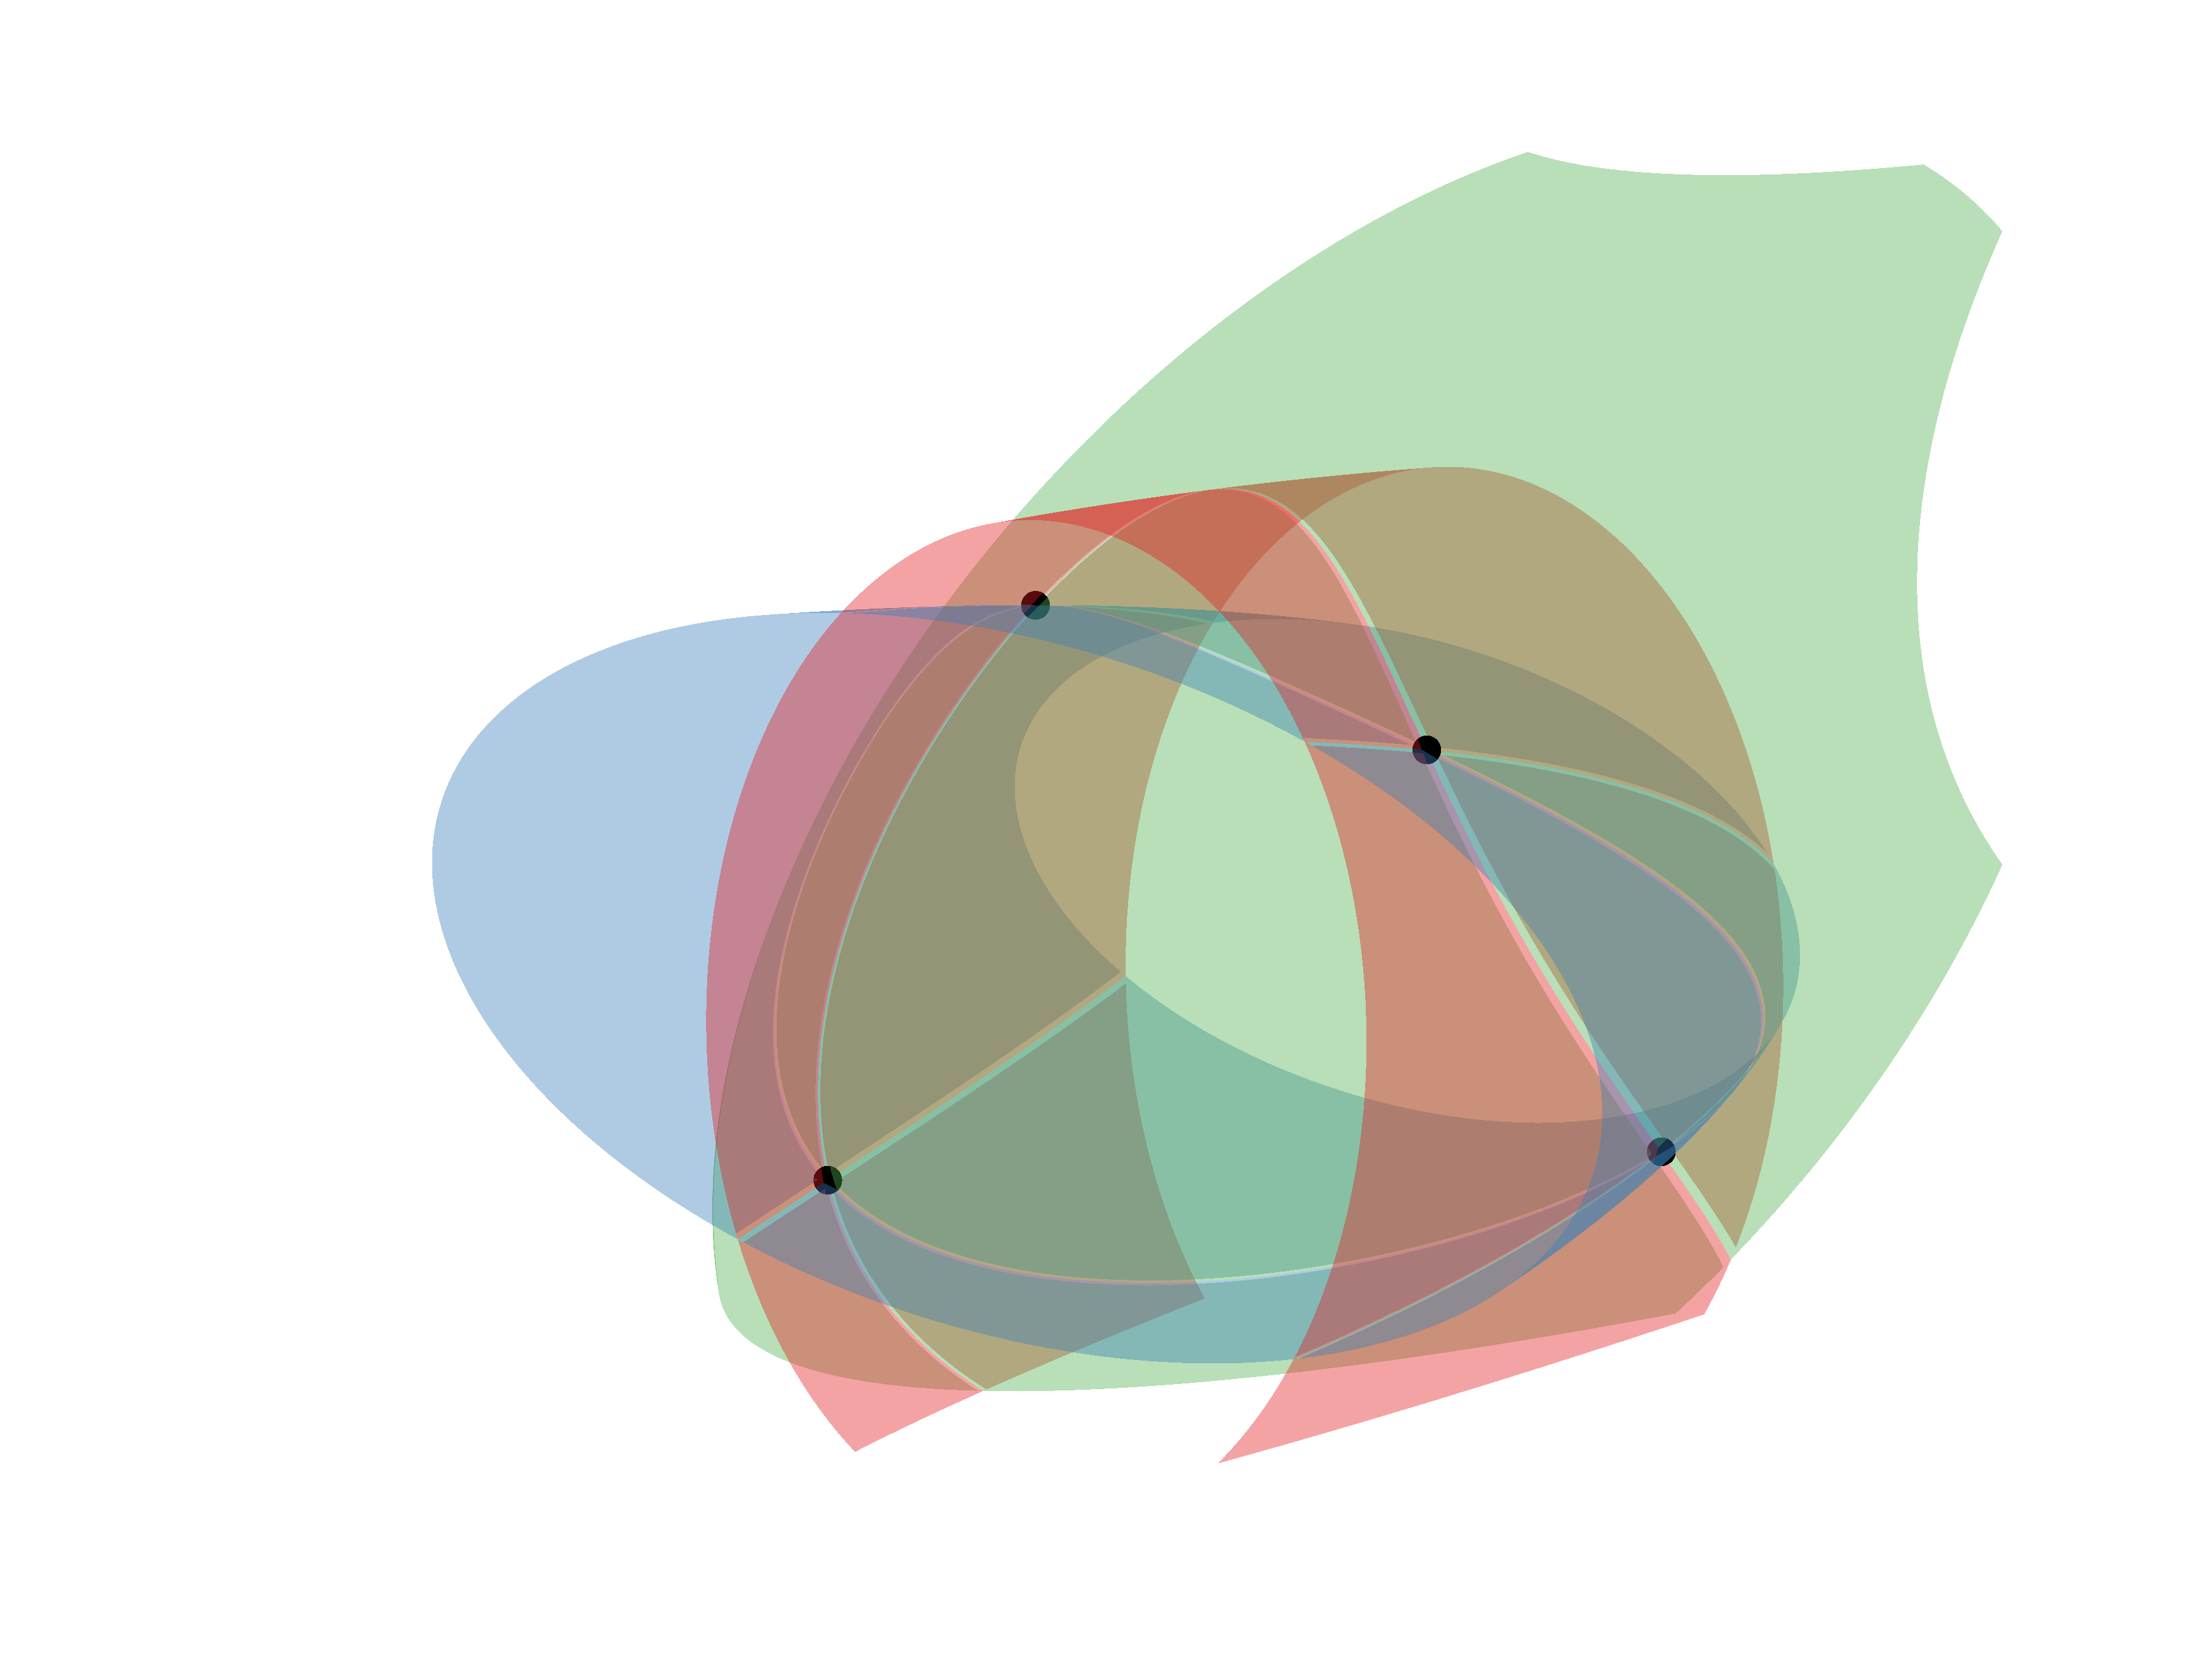
\includegraphics[width=0.8\textwidth]{"images/e3q3_example1_zoom.png"}
		\caption*{Schnittpunkte dreier Ellipsoide als Ergebnis des E3Q3-Algorithmus}
	\end{figure}
	\newpage
	\pagenumbering{Roman}
	\setcounter{tocdepth}{3}
	\tableofcontents
	\newpage
	\setcounter{tocdepth}{2}
	\listoffigures
	\newpage

	\pagestyle{fancy}
	\pagenumbering{arabic} 
	\section{Motivation}\label{chp:Motivation}
	In vielen Anwendungsfeldern der Mathematik kommen Problemstellungen vor, welche in Form eines Gleichungssystems aus drei Polynomen zweiten Grades in drei Unbekannten (3Q3) formuliert werden können. Für diesen Fall existieren bereits verschiedene Algorithmen zur Lösung der Gleichungssysteme. Diese sind in Bereichen wie der Computervision und der Robotik von großer Bedeutung, da sie beispielsweise zur Modellierung von Kamerapositionen oder Bewegungsabläufen verwendet werden. Auch in anderen Disziplinen, in denen geometrische Zusammenhänge eine Rolle spielen, finden diese Methoden Anwendung.\\
	
	Aufgrund der Anwendungsfelder sind diese Algorithmen für die reellen Zahlen formuliert, jedoch lässt sich der E3Q3-Algorithmus von Kukelova et al. \cite{kukelova2016efficient} mithilfe von algebraischer Geometrie auf beliebige Körper anwenden.\\
	
	Daraus ergeben sich zwei zentrale Fragestellungen, denen wir in dieser Arbeit nachgehen möchten. Zum einen wollen wir untersuchen, inwieweit der E3Q3-Algorithmus auch auf anderen Körpern, insbesondere auf endlichen Primkörpern, erfolgreich eingesetzt werden kann. Zum anderen stellt sich die Frage, ob das grundlegende Vorgehen dieses Algorithmus auf Gleichungssysteme mit kubischen Polynomen übertragen werden kann.
	\newpage
	\section{Das 3Q3-Problem und algebraische Geometrie}
	\subsection{Das 3Q3-Problem}
	Wie bereits erwähnt kommen in vielen Anwendungsfeldern der Mathematik Problemstellungen vor, welche in Form eines Gleichungssystems aus drei quadratischen Polynomen in drei Unbekannten formuliert werden können.
	
	\begin{definition}[3Q3-Problem]\label{def:3Q3}
		Sei $K$ ein Körper und seien $X_1$,$X_{2}$ und $X_{3}$ die Unbestimmten unseres Gleichungssystems. Weiter bezeichne $C \in K^{3\times 10}$ die Koeffizientenmatrix. Das Gleichungssystem, welches es zu lösen gilt, lautet dann
		\begin{gather}\label{eqn:3Q3}
			\begin{alignedat}{4}
				c_{1,1}X_{1}^2&+c_{1,2}X_{1}X_{2}+c_{1,3}X_{1}X_{3}+c_{1,4}X_{2}^2+c_{1,5}X_{2}X_{3}\ldots&&&\\&+c_{1,6}X_{3}^2+c_{1,7}X_{1}+c_{1,8}X_{2}+c_{1,9}X_{3}+c_{1,10}=0,\\
				c_{2,1}X_{1}^2&+c_{2,2}X_{1}X_{2}+c_{2,3}X_{1}X_{3}+c_{2,4}X_{2}^2+c_{2,5}X_{2}X_{3}\ldots&&&\\&+c_{2,6}X_{3}^2+c_{2,7}X_{1}+c_{2,8}X_{2}+c_{2,9}X_{3}+c_{2,10}=0,\\
				c_{3,1}X_{1}^2&+c_{3,2}X_{1}X_{2}+c_{3,3}X_{1}X_{3}+c_{3,4}X_{2}^2+c_{3,5}X_{2}X_{3}\ldots&&&\\&+c_{3,6}X_{3}^2+c_{3,7}X_{1}+c_{3,8}X_{2}+c_{3,9}X_{3}+c_{3,10}=0.\\
			\end{alignedat}
		\end{gather}
	\end{definition}
	Betrachten wir das 3Q3-Problem über dem Körper der reellen Zahlen $\R$ offenbart sich eine anschauliche geometrische Interpretation des Gleichungssystems. Über den reellen Zahlen beschreibt jede der Gleichungen eine Quadrik im Raum und die Lösungen des 3Q3-Problems sind genau die Punkte, in denen sich alle drei Quadriken gemeinsam schneiden.
	
	\begin{figure}[H]
		\centering
		\begin{subfigure}[b]{0.5\textwidth}
			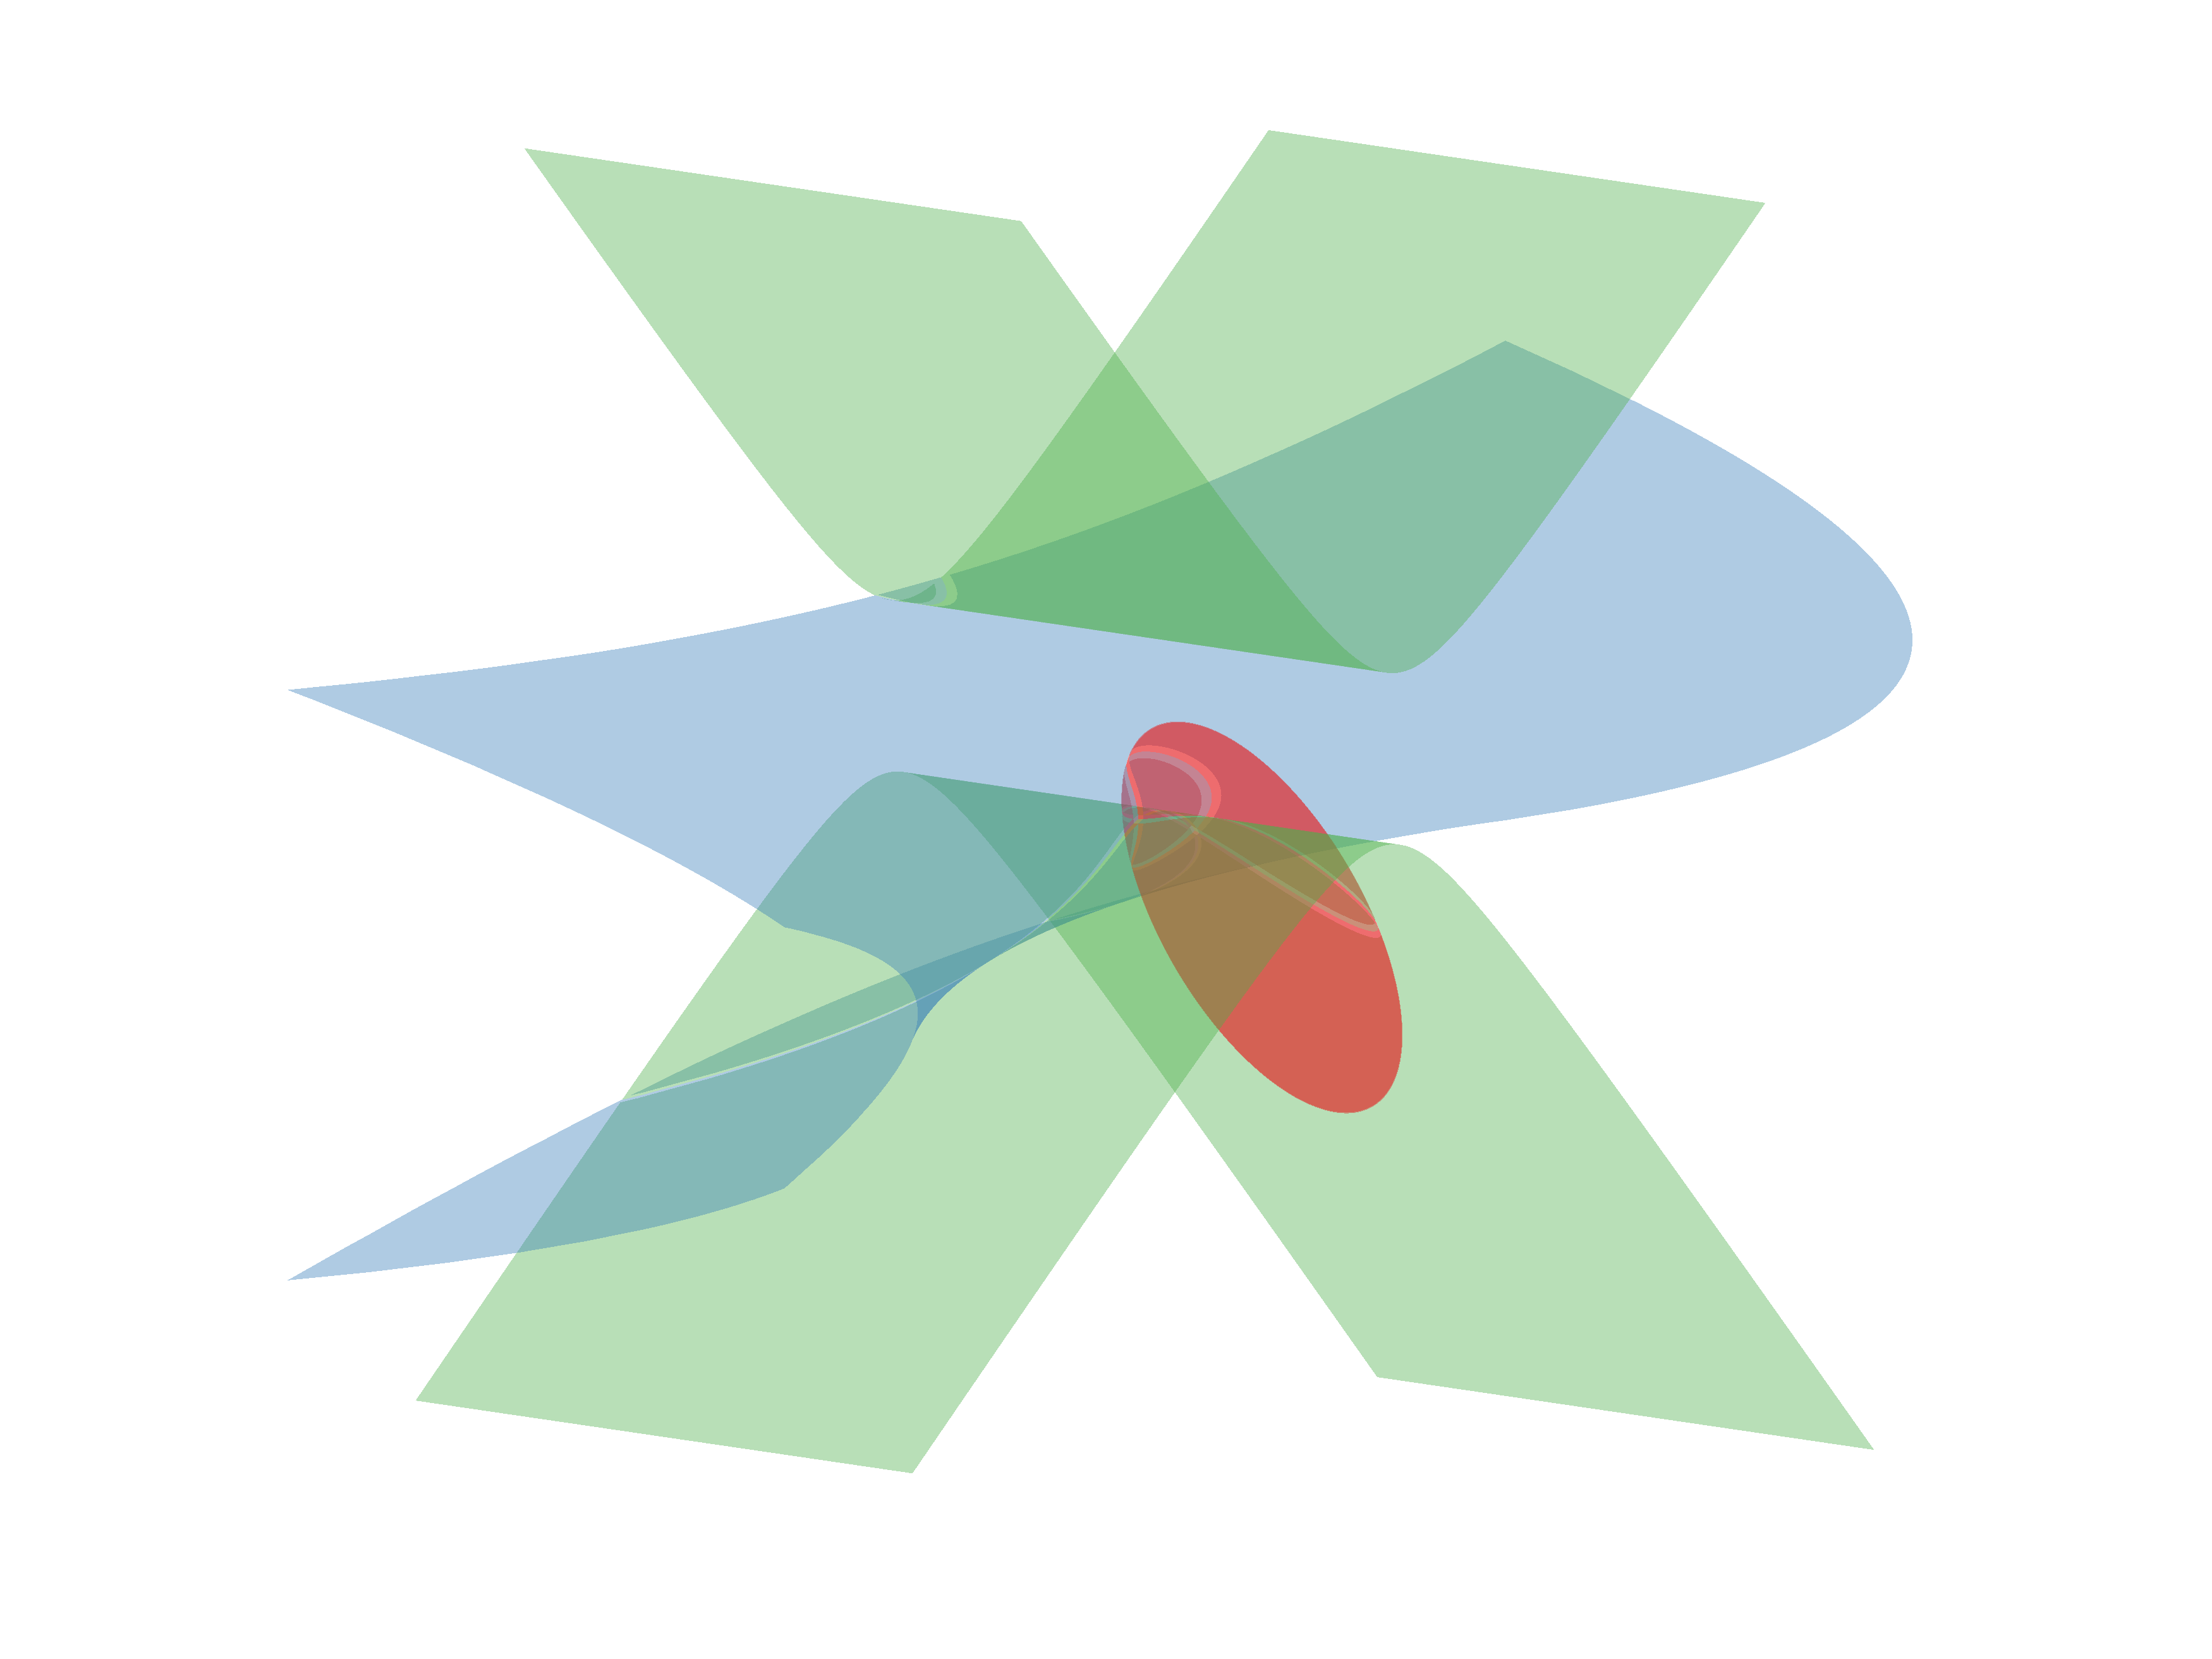
\includegraphics[width=\textwidth]{"images/3q3_example1.png"}
			\subcaption{Ein Ellipsoid (rot), ein hyperbolisches Paraboloid (blau) und ein hyperbolischer Zylinder (grün) über $\R$.}
		\end{subfigure}
			\end{figure}
				\begin{figure}[H]\ContinuedFloat
		\begin{subfigure}[b]{0.5\textwidth}
			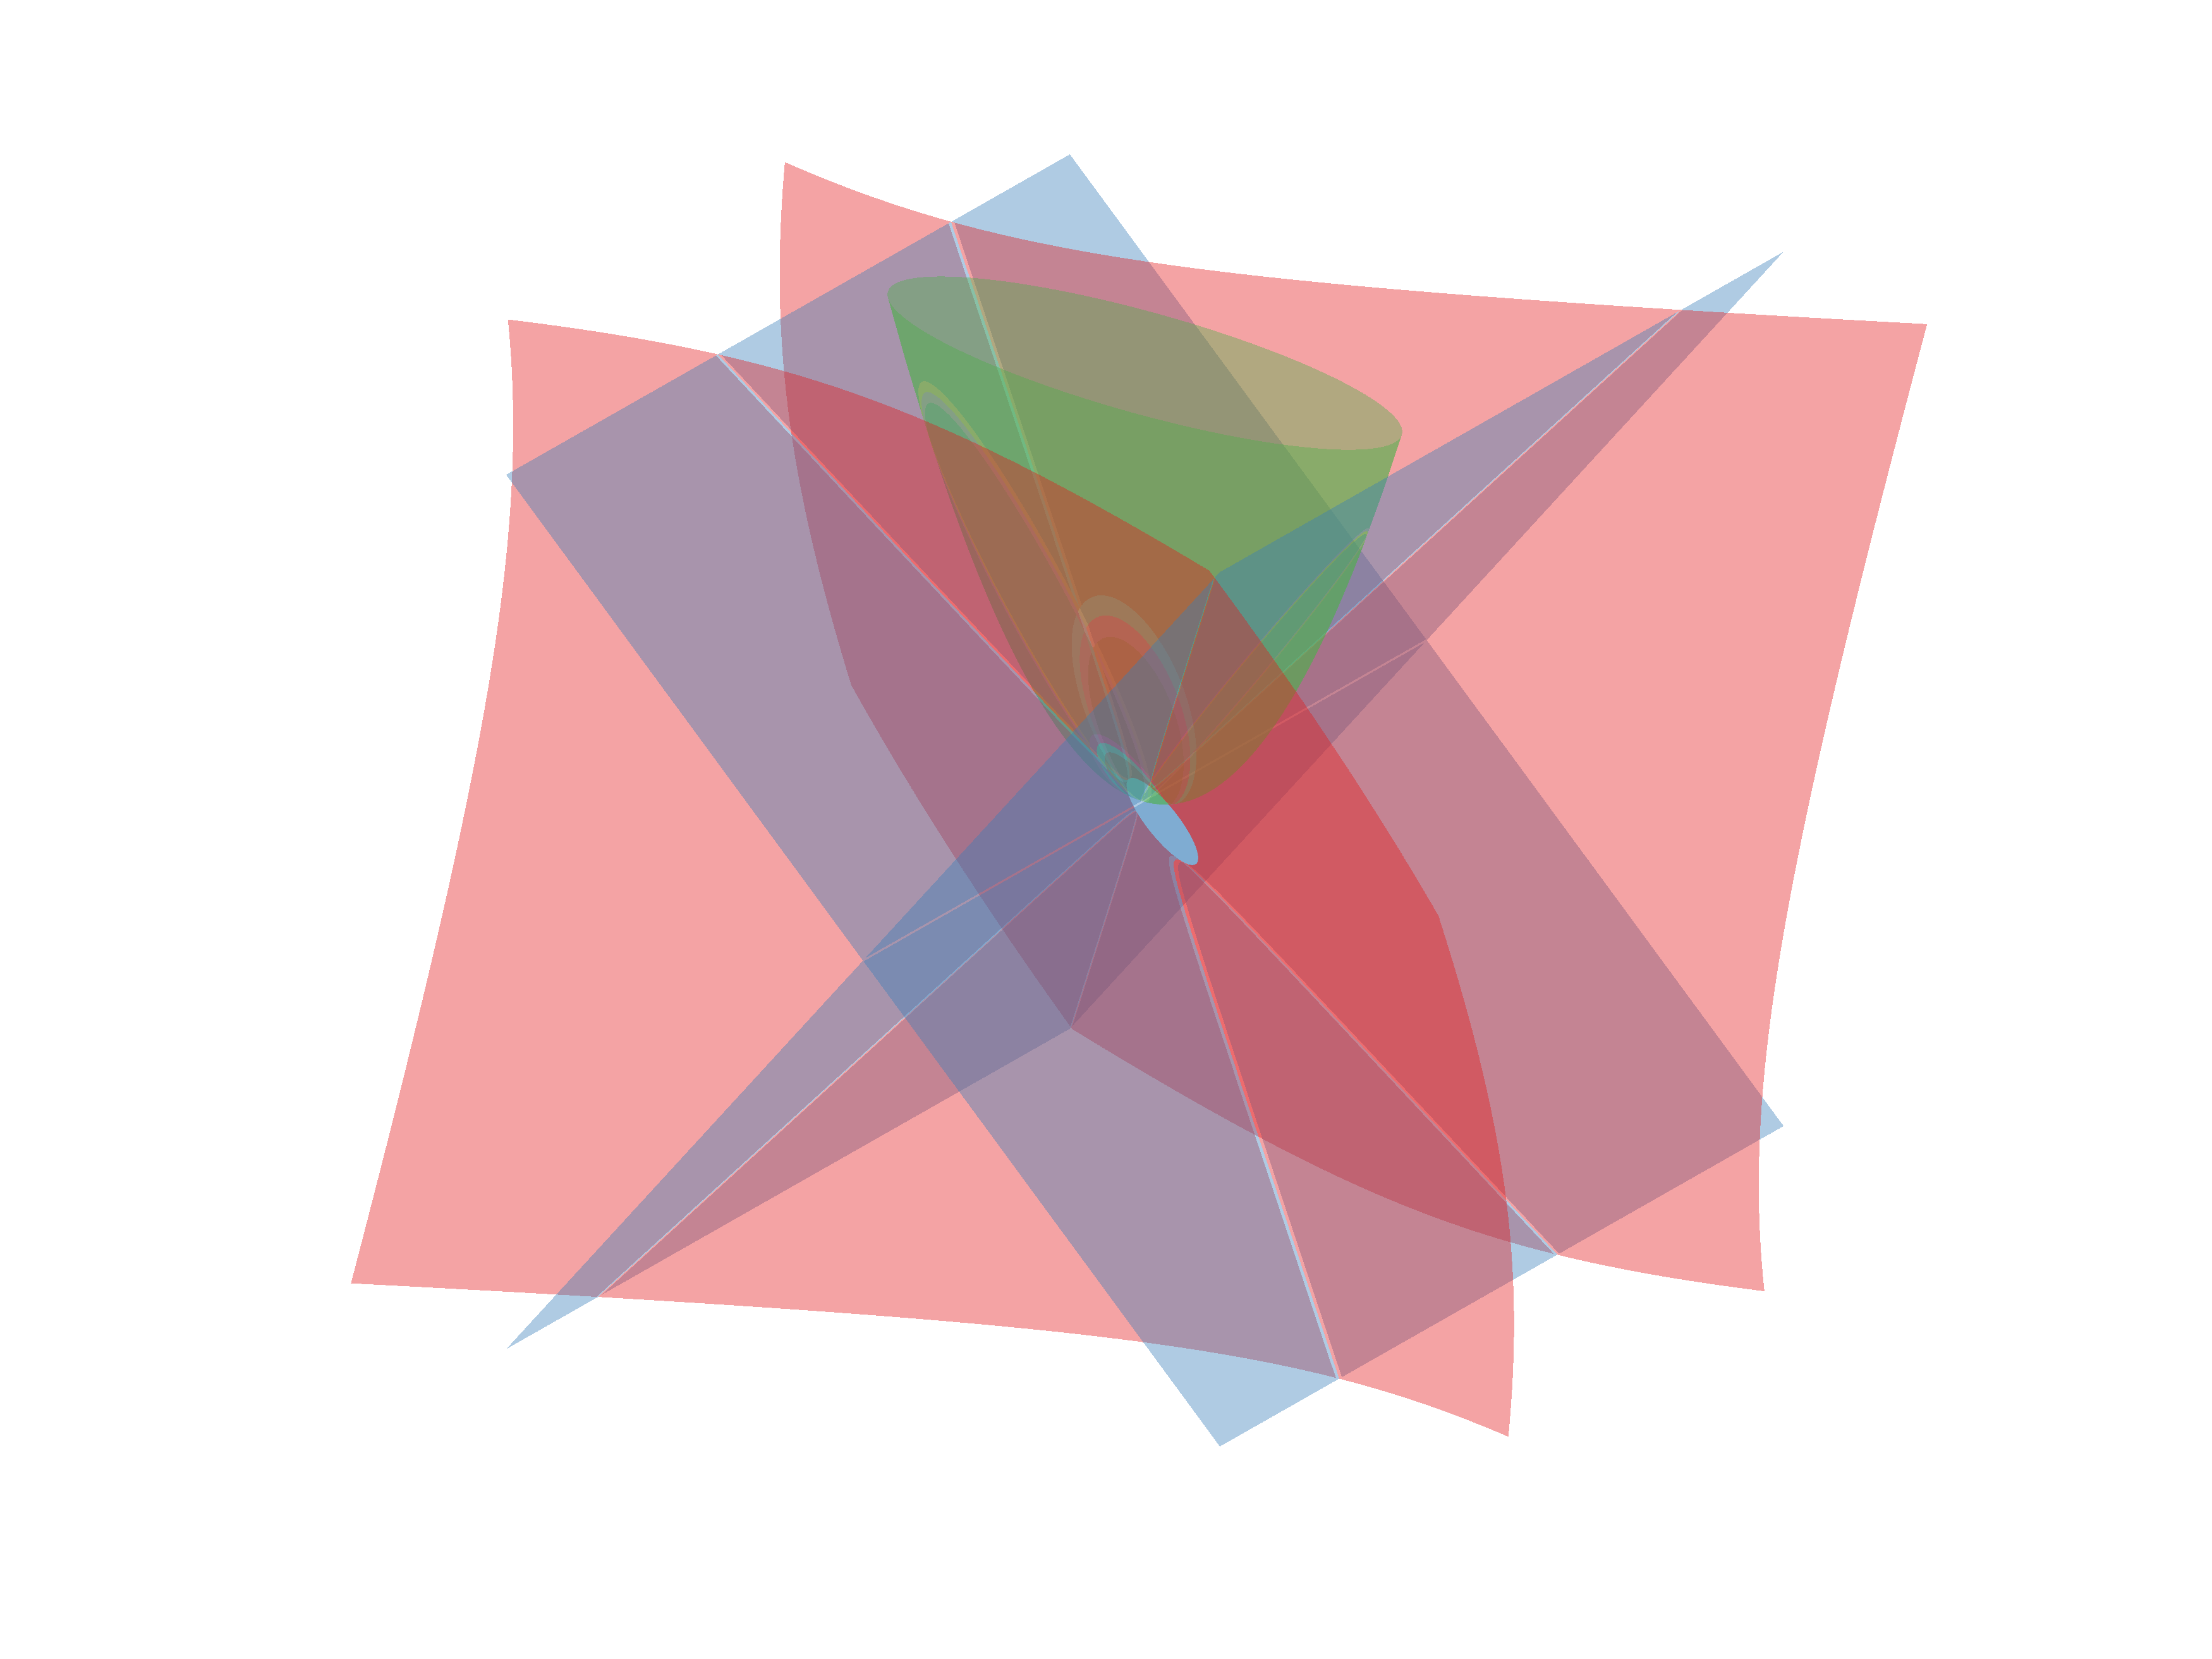
\includegraphics[width=\textwidth]{"images/3q3_example2.png"}
			\subcaption{Ein Hyperboloid erster Art (rot), zwei schneidende Ebenen (blau) und ein elliptisches Paraboloid (grün) über $\R$.}
		\end{subfigure}
		\caption{Geometrie zweier 3Q3-Probleme über den reellen Zahlen.}
	\end{figure}
	\subsection{Begriffe der algebraischen Geometrie}
	Aufgrund dieser geometrischen Interpretation des 3Q3-Problems werden wir das Gleichungssystem nun mithilfe der algebraischen Geometrie untersuchen. Dazu formulieren wir zuerst das 3Q3-Problem mit den entsprechenden Begriffen neu und orientieren uns dabei an Kunz \cite{kunz2012introduction,kunz2013}.
	
	\begin{definition}[Algebraisches Gleichungssystem {\cite{kunz2013}}]\label{def:alg_gs}
		Sei $K$ ein Körper, $m,n \in \N_{0}$ und $f_1,\ldots,f_m \in K\left[X_{1},\ldots,X_n\right]$ Polynome in den Unbestimmten $X_1,\ldots,X_n$. Ein algebraisches Gleichungssystem besitzt dann die Form
		\begin{equation}\label{eqn:alg_gs}
			\begin{alignedat}{5}
				&f_{1}&\left(X_{1}, \ldots, X_{n} \right)& \ &=\ &0,\\
				&f_{2}&\left(X_{1}, \ldots, X_{n} \right)& \ &=\ &0,\\
				&&&  \vdots& &\\
				&f_{m}&\left(X_{1}, \ldots, X_{n} \right)& \ &=\ &0.
			\end{alignedat}
		\end{equation}
	\end{definition} 
	Weiter sind wir interessiert an einer Formalisierung der Lösungsmenge algebraischer Gleichungssysteme und möglichen Aussagen über die Anzahl der Lösungen.
	
	\begin{definition}[Algebraische Menge]\label{def:alg_menge}
		Sei $K$ ein Körper und $\tilde{K}$ der zugehörige algebraische Abschluss.
		Eine Teilmenge $V \subset \tilde{K}^n$ zu einem Körper $K$ heißt affine, algebraische Menge, wenn es ein algebraisches Gleichungssystem gibt, so dass $V$ die Lösungsmenge des Systems ist. Das alg. Gleichungssystem nennt man das definierende Gleichungssystem von $V$ und man sagt $V$ sei definiert über $K$.
		Ist $L \subseteq \tilde{K}^{n}$ ein Erweiterungskörper von $K$, so nennt man die Elemente der Menge
		\begin{equation*}
			V_{L} \coloneqq V \cap L^{n}
		\end{equation*}
		die $L$-rationalen Punkte von $V$.
	\end{definition} 
	\begin{definition}[Algebraische Hyperfläche]
		Eine über dem Körper $K$ definierte, affine algebraische Hyperfläche ist eine Teilmenge $H \subset \tilde{K}^{n}$ mit der Gestalt
		\begin{equation}
			H = \{\left( \alpha_{1},\dots,\alpha_{n}\right) \in \tilde{K}^{n} \colon f\left(  \alpha_{1},\dots,\alpha_{n}\right) = 0  \} \ , 
		\end{equation}
		wobei $\tilde{K}^{n}$ den algebraischen Abschluss von $K$ bezeichnet und \newline ${f \in K\left[ X_{1},\dots, X_{n}\right] \setminus K}$ gilt. Man nennt $H$ die durch $f$ definierte Hyperfläche und $f$ ein $H$ definierendes Polynom.\\
		Ist $L \subseteq \tilde{K}^{n}$ ein Erweiterungskörper von $K$, so nennt man die Element der Menge
		\begin{equation*}
			H_{L} \coloneqq H \cap L^{n}
		\end{equation*}
		die $L$-rationalen Punkte von $H$.
	\end{definition}
	
	Nachdem wir die Lösungsmenge eines algebraischen Gleichungssystems definiert haben, widmen wir uns weiteren algebraischen Strukturen, um Erkenntnisse über die Kardinalität solcher Mengen zu erhalten.
	\begin{definition}[Ideal]
		Eine Teilmenge $I$ eines kommutativen Ringes $R$, welche die Bedingungen
		\begin{enumerate}
			\item $\forall \ i_1,\ i_2 \in I \colon i_1+i_2 \in I$  
			\item $\forall \ r \in R,\ i \in I \colon r \cdot i \in I$	
		\end{enumerate}
		erfüllt, wird als Ideal von $R$ bezeichnet.
	\end{definition}
	\begin{definition}
		Es seien $R$ ein kommutativer Ring und $I$ ein Ideal von $R$ mit $I \neq R$.
		\begin{enumerate}
			\item Wir nennen $I$ \textbf{maximal}, wenn es kein Ideal $J$ gibt mit $I \subsetneqq J \subsetneqq R$.
			\item Wir nennen $I$ \textbf{prim}, wenn aus $a\cdot b \in I$ stets $a \in I$ oder $b \in I$ folgt.
			\item Wir nennen $I$ \textbf{primär}, wenn aus $a\cdot b \in I$ mit $a \not\in I$ folgt, dass es ein $n \in \N$ gibt mit $b^n \in I$.
			\item $\text{Rad}(I) \coloneqq \sqrt{I} \coloneqq \{x \in R \ \left| \  \exists \, n \in \N \colon x^n \in I\right.\}$ ist ein Ideal von $R$ und wird als Radikal von $I$ bezeichnet.
		\end{enumerate}
	\end{definition}
	Diese Idealtypen spielen eine Schlüsselrolle in der Untersuchung von Lösungen algebraischer Gleichungssysteme.
	Schließlich können wir nach Masser \cite{masser1983fields} einen zentralen Satz formulieren, der eine Aussage über die Anzahl der Lösungen von algebraischen Gleichungssystemen trifft.
	\begin{proposition}\label{prop:bezout}
		Es seien $K$ ein algebraisch abgeschlossener Körper und $f_1,\ldots,f_m$ $\in$ \newline $K[X_1,\ldots,X_n]$ Polynome der Grade $d_1,\ldots,d_m \in \N$. Besitzt das algebraische Gleichungssystem
		\begin{equation*}
			\begin{alignedat}{5}
				&f_{1}&\left(X_{1}, \ldots, X_{n} \right)& \ &=\ &0\\
				&f_{2}&\left(X_{1}, \ldots, X_{n} \right)& \ &=\ &0\\
				&&&  \vdots& &\\
				&f_{m}&\left(X_{1}, \ldots, X_{n} \right)& \ &=\ &0
			\end{alignedat}
		\end{equation*}
		endlich viele Lösungen, so ist deren Anzahl höchstens gleich $d_1 \cdot \ldots \cdot d_m$.
	\end{proposition}
	Um diesen Satz zu beweisen benötigen wir noch einige Definitionen und Resultate.\\
	Es sei $J \coloneqq (f_1,\ldots,f_m)$ das von den Polynomen aus Satz \ref{prop:bezout} erzeugte Ideal von $K[X_1,\ldots,X_n]$.
	Nach dem Hilbert'schen Nullstellensatz liefert die Zuordnung
	\begin{equation*}
		(a_1,\ldots,a_n) \in K^n \mapsto (X_1 - a_1, \ldots,X_n - a_n)
	\end{equation*}
	eine bijektive Abbildung der Lösungen eines Polynomgleichungssystems auf diejenigen maximalen Ideale von $K[X_1,\ldots,X_n]$, die $J$ enthalten. Es genügt also die Kardinalität der Menge
	\begin{equation*}
		\{p \subset K[X_1,\ldots,X_n] \colon J \subseteq p, p \ \text{maximal}\}
	\end{equation*}
	zu bestimmen.\\
	Zwischen Prim-, Primäridealen und maximalen Idealen bestehen nach Kunz \cite{kunz2013,kunz2012introduction} außerdem die folgenden Beziehungen.
	\begin{lemma}\label{cor:prim_max}
		Es sei $I$ ein primäres Ideal eines kommutativen Ringes $R$, dann ist $\sqrt{I}$ prim.
	\end{lemma}

	\begin{lemma}
		Sei $q$ ein primäres Ideal mit $J \subseteq q$, so ist $\sqrt{q}$ ein maximales Ideal.
	\end{lemma}
	
	\begin{theorem}[Lasker-Noether]
		Jedes Ideal $I$ eines Polynomrings $K[X_1,\ldots,X_n]$ besitzt eine Darstellung
		\[I = q_1 \cap \ldots \cap q_r\]
		als Schnitt primärer Ideale $q_i$ für die Folgendes gilt:
		\begin{enumerate}
			\item Kein $q_i$ kann weggelassen werden.
			\item Die Primideale $\sqrt{q_1}, \ldots, \sqrt{q_r}$ sind paarweise verschieden.
		\end{enumerate}
		Die Primideale $\sqrt{q_i}$ (aber nicht die Ideale $q_i$) sind dabei durch $I$ eindeutig bestimmt. Die Ideale $q_i$ heißen Primärkomponenten von $I$.
	\end{theorem}
	\begin{proof}
		Siehe Kunz \cite{kunz2012introduction}.
	\end{proof}
	\begin{definition}
		Eine Primärkomponente $q_i$ eines Ideal $I \subset K[X_1,\ldots,X_n]$ heißt isoliert, falls das Primideal $\sqrt{q_i}$ in keinem der Primideale $\sqrt{q_j}$ enthalten ist.
	\end{definition}
	\begin{definition}
		Die Höhe (in Masser \cite{masser1983fields} mit Rang bezeichnet) eines Primideals $p$ von $K[X_1,\ldots,X_n]$ ist die Länge $l$ der längsten Kette \[0=p_0 \subset p_1 \subset \ldots \subset p_l = p\] von Primidealen $p_i$. Es gilt $l \leq n$ mit Gleichheit genau dann, wenn $p$ ein maximales Ideal ist.
	\end{definition}
	\begin{lemma}\label{cor:gls_prim_max}
		Im Fall des Ideals $J$ zum Polynomgleichungssystem aus Satz \ref{prop:bezout} sind alle
		Primärkomponenten isoliert, denn nach Korollar \ref{cor:prim_max} sind  die Primideale $\sqrt{q_i}$ alle maximal. Die Menge $\{\sqrt{q_1},\ldots,\sqrt{q_r}\}$ besteht sogar aus allen maximalen Idealen, welche $J$ enthalten.
	\end{lemma}
	\begin{proof}
		Seien $P_1, \ldots, P_r \in K^n$ die Lösungen des Polynomgleichungssystems aus Satz \ref{prop:bezout}, so gilt nach dem Hilbert'schen Nullstellensatz \cite{kunz2013}
		\begin{equation*}
			I_\mathcal{V}(P_1) \cap \ldots \cap I_\mathcal{V}(P_r) = \sqrt{J}.
		\end{equation*}
		Andererseits gilt auch
		\begin{equation*}
			\sqrt{J} = \sqrt{q_1} \cap \ldots \cap \sqrt{q_r}.
		\end{equation*}
	\end{proof}
	\begin{definition}
		Die Länge $l(q)$ eines Primärideals $q \subset K[X_1,\ldots,X_n]$ ist wie folgt definiert: Man bildet den Bruchring \[R_p \coloneqq \left\lbrace \frac{z}{n} \colon z \in  K[X_1,\ldots,X_n], n \in  K[X_1,\ldots,X_n] \setminus q \right\rbrace.\]
		Für jedes Ideal $J \subset K[X_1,\ldots,X_n], J \subseteq p$, ist die Menge \[JR_p \coloneqq \{a\cdot r \colon a \in J, r \in R_p\}\]
		ein Ideal von $R_p$.\\
		$pR_p$ ist ein maximales Ideal von $R_p$ und die Länge der längsten Kette \[J_0 \coloneqq qR_p \subset J_1 \subset \ldots \subset J_l \coloneqq pR_p\] ist die zu definierende Länge $l(q)$.
	\end{definition}
	\begin{definition}
		Ist $J \subseteq K[X_1,\ldots,X_n]$ ein Ideal, das eine Darstellung $J = q_1 \cap \ldots \cap q_r$ als Schnitt von isolierten Primäridealen $q_i$ besitzt, so ist die Länge von $J$ definiert als \[l(J) \coloneqq \sum_{i=1}^{r} l(q_i).\]
	\end{definition}
	\begin{proof}[Beweis zu Satz \ref{prop:bezout}]
		Es sei \[I \coloneqq (f_1, \ldots, f_m) = q_1 \cap \ldots \cap q_r\] eine Darstellung von $I$ nach dem Satz von Lasker-Noether. Nach sind alle Primärkomponenten $q_i$ isoliert, womit die Länge von $I$ definiert ist. Nach Definition gilt \[l(I) = \sum_{i=1}^{r} l(q_i)\geq r\] und nach dem Hilbert'schen Nullstellensatz und \ref{cor:gls_prim_max} ist $r$ die Anzahl verschiedener Lösungen der algebraischen Gleichungssystems. Man wendet nun das Korollar für den Fall $s=n$ an, da die Primideale $\sqrt{q_i}$ maximal sind, also den Rang $n$ besitzen. Es ist $t \leq m$ und damit \[M_t(d_1, \ldots, d_m) \leq d_1 \cdot \ldots \cdot d_m,\] woraus die Aussage des Satzes folgt.
	\end{proof}
	\newpage
	\section{Lösen des 3Q3-Problems}\label{chp:3Q3}

	
	\subsection[Der E3Q3-Algorithmus]{Der E3Q3-Algorithmus~\cite{kukelova2016efficient}}\label{sec:E3Q3}
	Es liege nun das 3Q3-Problem in der Form
	\begin{equation*}
		\begin{pmatrix}
			c_{1,1}&c_{1,2}&\ldots&c_{1,10}\\
			c_{2,1}&c_{2,2}&\ldots&c_{2,10}\\
			c_{3,1}&c_{3,2}&\ldots&c_{3,10}\\
		\end{pmatrix} \cdot
		\begin{pmatrix}
			X_{1}^{2},X_{1}X_{2},X_{1}X_{3},X_{2}^{2},X_{2}X_{3},X_{3}^{2},X_{1},X_{2},X_{3},1
		\end{pmatrix}^\top =  \begin{pmatrix}
		 0\\0\\0
		\end{pmatrix}
	\end{equation*}
	vor.\\
	Im ersten Schritt wechseln wir bei der Betrachtung des Gleichungssystems über $K\left[X_{1},X_{2},X_{3}\right]$ zu $K\left[X_{1}\right] \left[ X_{2},X_{3}\right]$. Wir \glqq verstauen\grqq~ die Unbestimmte $X_{1}$ erstmal im Koeffizientenbereich und arbeiten über dem Polynomring in den Unbestimmten $X_{2}$ und $X_{3}$.\\
	Daraus ergibt sich das algebraische Gleichungssystem 
	\begin{equation}\label{eqn:E3Q3}
\begin{alignedat}{6}
			&p_{11}^{\left[1\right] }\left(X_{1}\right)X_{2}+
			&p_{12}^{\left[1\right] }\left(X_{1}\right)X_{3}+
			&p_{13}^{\left[2\right] }\left(X_{1}\right)+
			&c_{14}X_{2}^2+&c_{15}X_{2}X_{3}+&c_{16}X_{3}^2=0,\\
			&p_{21}^{\left[1\right] }\left(X_{1}\right)X_{2}+
			&p_{22}^{\left[1\right] }\left(X_{1}\right)X_{3}+
			&p_{23}^{\left[2\right] }\left(X_{1}\right)+
			&c_{24}X_{2}^2+&c_{25}X_{2}X_{3}+&c_{26}X_{3}^2=0,\\
			&p_{31}^{\left[1\right] }\left(X_{1}\right)X_{2}+
			&p_{32}^{\left[1\right] }\left(X_{1}\right)X_{3}+
			&p_{33}^{\left[2\right] }\left(X_{1}\right)+
			&c_{34}X_{2}^2+&c_{35}X_{2}X_{3}+&c_{36}X_{3}^2=0,
\end{alignedat}
	\end{equation}
	wobei $c_{ij} \in K$ und $p_{ij}^{\left[\cdot \right] } \in K\left[ X_{1}\right]$ gilt und der obere Index $\left[\cdot \right]$ den Maximalgrad des Polynoms darstellt.\\
	Durch Aufteilen der Unbestimmten in zwei Gruppen $G_1 \coloneqq \{X_{2}^2,X_{2}X_{3},X_{3}^2\}$ und $G_2 \coloneqq \{X_{2},X_{3},1\}$ erhält man
	\begin{equation}\label{eqn:E3Q3_sep}
		- \ 
		C \
		\begin{pmatrix}
			X_{2}^2\\X_{2}X_{3}\\X_{3}^2
		\end{pmatrix} 
		=
		P \
		\begin{pmatrix}
			X_{2}\\X_{3}\\1
		\end{pmatrix},
	\end{equation}
	mit den Matrizen
	\begin{equation}
		C = \begin{pmatrix}
			c_{14}&c_{15}&c_{16}\\
			c_{24}&c_{25}&c_{26}\\
			c_{34}&c_{35}&c_{36}\\
		\end{pmatrix} \in K^{3 \times 3}
	\end{equation}
	und
	\begin{equation}
		P = \begin{pmatrix}
			p_{11}\left(X_{1}\right)&p_{12}\left(X_{1}\right)&p_{13}\left(X_{1}\right)\\
			p_{21}\left(X_{1}\right)&p_{22}\left(X_{1}\right)&p_{23}\left(X_{1}\right)\\
			p_{31}\left(X_{1}\right)&p_{32}\left(X_{1}\right)&p_{33}\left(X_{1}\right)\\
		\end{pmatrix} \in K[X_1]^{3 \times 3}
	\end{equation}
	erhält.\\
	Wir setzen nun voraus, dass $C$ invertierbar ist und können so Gleichung \eqref{eqn:E3Q3_sep} von links mit $C^{-1}$ ausmultiplizieren. Dies führt zu dem Gleichungssystem
	\begin{equation}\label{eqn:E3Q3_inv}
			\begin{pmatrix}
			X_{2}^2\\X_{2}X_{3}\\X_{3}^2
		\end{pmatrix} 
		=
		\begin{pmatrix}
		p'_{11}\left(X_{1}\right)&p'_{12}\left(X_{1}\right)&p'_{13}\left(X_{1}\right)\\
		p'_{21}\left(X_{1}\right)&p'_{22}\left(X_{1}\right)&p'_{23}\left(X_{1}\right)\\
		p'_{31}\left(X_{1}\right)&p'_{32}\left(X_{1}\right)&p'_{33}\left(X_{1}\right)\\
		\end{pmatrix}
		\begin{pmatrix}
			X_{2}\\X_{3}\\1
		\end{pmatrix}
		,
	\end{equation}
	wobei die Polynome $p'_{ij}\left(X_{1}\right) \in K[X_{1}]$ aus Linearkombinationen der Polynome $p_{ij}\left(X_{1}\right)$ bestehen und sich somit die Maximalgrade aus Gleichung \eqref{eqn:E3Q3} von $p_{ij}\left(X_{1}\right)$ auf $p'_{ij}\left(X_{1}\right)$ übertragen.\\
	Mithilfe von Gleichung \eqref{eqn:E3Q3_inv} lassen sich die quadratischen Monome $X_{2}^2$, $X_{3}^2$ und $X_{2}X_{3}$ durch Linearkombinationen aus den Monomen $X_{2}$,$X_{3}$,$1$ mit Koeffizienten in $K\left[X_{1}\right] $ schreiben.
	
	Um dies auszunutzen betrachten wir zunächst drei Identitäten in den Monomen $X_{2}^2$, $X_{3}^2$ und $X_{2}X_{3}$:
	\begin{equation}
		\begin{alignedat}{-1}
			&\left(X_{2}^2\right) &X_{3}\ & &=& &\Bigl(X_{2}X_{3} \Bigr)&  X_{2},\\
			&\left(X_{3}^2\right) &X_{2}\ & &=& &\Bigl(X_{2}X_{3} \Bigr)&  X_{3},\\
			&\left(X_{2}^2\right) &\left( X_{3}^2\right)&  &=& &\Bigl(X_{2}X_{3} \Bigr)&  \Bigl(X_{2}X_{3} \Bigr).
		\end{alignedat}
	\end{equation}
	
	Da die Substitutionen für $X_{2}^2$, $X_{3}^2$ und $X_{2}X_{3}$ aus Linearkombinationen in $X_{2}$ und $X_{3}$ bestehen, erhalten wir nach der ersten Substitution das Gleichungssystem
	\begin{equation}
		\begin{alignedat}{1}
			p'_{11}X_{2}X_{3}+p'_{12}X_{3}^2+p'_{13}X_{3}&=p'_{21}X_{2}^2+p'_{22}X_{2}X_{3}+p'_{23}X_{2},\\
			p'_{31}X_{2}^2+p'_{32}X_{2}X_{3}+p'_{33}X_{2}&=p'_{21}X_{2}X_{3}+p'_{22}X_{3}^2+p'_{23}X_{3},\\
			\left(p'_{21}X_{2}+p'_{22}X_{3}+p'_{23}\right)^2&=\left( p'_{11}X_{2}+p'_{12}X_{3}+p'_{13}\right)\\ & \quad \cdot \left( p'_{31}X_{2}+p'_{32}X_{3}+p'_{33}\right),
		\end{alignedat}
	\end{equation}
	wobei die $p'_{ij} \in K[X_{1}]$ die Polynome aus Gleichung \eqref{eqn:E3Q3_inv} sind.
	Da im Gleichungssystem wieder Terme in den Monomen $X_{2}^2$,$X_{2}X_{3}$,$X_{3}^2$ vorkommen,
	führt ein weiteres Substituieren auf ein Gleichungssystem der Form
	\begin{equation}\label{eqn:E3Q3_M_eq}
		\begin{pmatrix}[1.5]
			m_{11}^{\left[ 2\right]}\left( X_{1}\right) & m_{12}^{\left[ 2\right]}\left( X_{1}\right) & m_{13}^{\left[ 3\right]}\left( X_{1}\right) \\
			m_{21}^{\left[ 2\right]}\left( X_{1}\right) & m_{22}^{\left[ 2\right]}\left( X_{1}\right) & m_{23}^{\left[ 3\right]}\left( X_{1}\right) \\
			m_{31}^{\left[ 2\right]}\left( X_{1}\right) & m_{32}^{\left[ 2\right]}\left( X_{1}\right) & m_{33}^{\left[ 3\right]}\left( X_{1}\right) \\
		\end{pmatrix}
		\begin{pmatrix}[1.5]
			X_{2}\\
			X_{3}\\
			1
		\end{pmatrix}
		= M\left( X_{1}\right) \ \begin{pmatrix}[1.5]
			X_{2}\\
			X_{3}\\
			1
		\end{pmatrix}
		=0,
	\end{equation}
	wobei $m_{ij}^{\left[\cdot \right] }\left(X_{1}\right) \in K\left[ X_{1}\right]$ gilt und der obere Index $\left[\cdot \right]$ den Maximalgrad des Polynoms darstellt.\\
	Die Identitäten müssen so gewählt sein, dass in den Substitutionsschritten keine Terme höherer Ordnung in $K[X_1][X_2,X_3]$ entstehen und wir brauchen so viele Identitäten, wie wir Monome in $G_2$ haben um am Ende die Matrixgleichung \eqref{eqn:E3Q3_M_eq} zu erhalten.
	
	

	\begin{proposition}\label{prop:LGS}
		Sei $K$ ein Körper und $A \in K^{n \times n}$ eine Matrix. 
		Dann besitzt das lineare Gleichungssystem $A\cdot x = 0_{K^{n}}$ nichttriviale Lösungen $x$ genau dann, wenn $\det(A)=0$ gilt.
	\end{proposition}
	\begin{proof}Wir beweisen zunächst durch Kontraposition.\\
		${\glqq \Rightarrow \grqq}$ Sei $\det(A)\neq0$, so existiert die zu $A$ inverse Matrix $A^{-1}$. Es folgt
		\begin{equation*}
			A\cdot x = 0_{K^{n}} \quad \Leftrightarrow \quad A^{-1}\cdot A \cdot x = A^{-1}\cdot 0_{K^{n}} \quad \Leftrightarrow\quad  x = 0_{K^{n}}
		\end{equation*}
		${\glqq \Leftarrow \grqq}$ Sei $\det(A)=0$, die Spaltenvektoren $a_{j}$ also linear abhängig. Durch Aufteilen auf die Spaltenvektoren erhalten wir
		\begin{equation*}
			A\cdot x = a_{1}x_1+a_{2}x_2+\ldots+a_{n}x_n=0_{K^{n}}
		\end{equation*}
		Da die Spaltenvektoren $a_{j}$ linear abhängig sind ist $x$ nach Definition der linearen Unabhängigkeit also eine nichttriviale Lösung des Gleichungssystems.
	\end{proof}
	
	Folglich besitzt das lineare Gleichungsystem nichttriviale Lösungen $x_2$ und $x_3$ genau dann, wenn $M\left( X_{1}\right)$ als polynomiale Matrix über $K[X_{1}]^{3 \times 3}$ regulär ist und \begin{equation}\label{eqn:det_zero}
		\det\left(M\left( X_{1}\right)  \right) = 0
	\end{equation}
	erfüllt ist.\\
	Wir ermitteln also zunächst die (bis zu) 8 Lösungen $\tilde{x}_{1} \in K$ von Gleichung \eqref{eqn:det_zero}, welche gleichzeitig die Lösungskandidaten der Unbestimmten $X_{1}$ aus der ursprünglichen Gleichungssystems \eqref{eqn:E3Q3} darstellen. Die zugehörigen Lösungen $x_{2}$ und $x_{3}$ erhält man durch Einsetzen der Nullstelle $\tilde{x}_{1}$ in die Matrix $M\left( X_1\right) $.
	Für die resultierende Matrix $ \tilde{M} \coloneqq M(\tilde{x}_{1})$ gilt $\text{rank}\left(\tilde{M}\right) < 3$ und durch Lösen des zugehörigen Gleichungssystems
	\begin{equation}\label{eqn:M_lsg}
		\begin{pmatrix}
			\tilde{m}_{11} & \tilde{m}_{12}\\
			\tilde{m}_{21} & \tilde{m}_{22}\\
			\tilde{m}_{31} & \tilde{m}_{32}\\
		\end{pmatrix}
		\begin{pmatrix}[1.5]
			X_{2}\\
			X_{3}
		\end{pmatrix}
		= -\ \begin{pmatrix}
			\tilde{m}_{13}\\
			\tilde{m}_{23}\\
			\tilde{m}_{33}
		\end{pmatrix}
	\end{equation}
	erhält man die zu $\tilde{x}_{1}$ zugehörigen Lösungen $\tilde{x}_{2}$ und $\tilde{x}_{3}$.\\
	Falls die Matrix $\tilde{M}$ den Rang 1 hat erhalten wir die Lösungen nicht direkt, sondern erst eine Gleichung der Form 
	\begin{equation}\label{eqn:3Q3_r1}
		a X_2 + b X_3 + c = 0,
	\end{equation}
	mit $a,b,c \in K$, wobei nicht $a=b=0$ gelten kann.
	Diese können wir nun nach einer Unbestimmten auflösen und in Originalgleichungssystem zusammen mit $\tilde{x}_1$ einsetzen. Es resultieren 3 konsistente quadratische Gleichungen in der fehlenden Variable. Nach dieser können wir nun auflösen und erhalten durch die Beziehung \eqref{eqn:3Q3_r1} die vollständige Lösung.
	Hat die Matrix den Rang 2 so stellt des Gleichungssystem \eqref{eqn:M_lsg} ein quadratisches Gleichungssystem dar und liefert somit eine eindeutige Lösung $(\tilde{x}_{2},\tilde{x}_{3})$.
	\begin{remarks}
		~\begin{enumerate}
			\item Da $K[X_1,X_2,X_3] = K[X_1][X_2,X_3] = K[X_2][X_1,X_3] = K[X_3][X_1,X_2]$ gilt, erhalten wir drei verschiedene Wege den Algorithmus durchzuführen.
			\item Die geforderte Regularität der Matrix $A$ bedeutet, dass die drei Polynome echte quadratische Polynome über $K[X_1][X_2,X_3]$ sind, deren quadratische Koeffizienten $(c_{i4},c_{i5},c_{i6})$ für $i \in \{1,2,3\}$ linear unabhängig sein müssen.
			
			\item Das Vorkommen der Lösungen als Nullstellen eines Polynom achten Grades lässt sich durch Satz \ref{prop:bezout} auch mit algebraischer Geometrie erklären. Da durch die geforderte Regularität der Matrix $M(X_1) \in K[X_1]^{3 \times 3}$ unendlich viele Lösungen ausgeschlossen werden, ergibt sich aus Satz \ref{prop:bezout} die maximale Anzahl an Lösungen als $2^3=8$.
			\item Ist $\tilde{M}$ eine reelle Matrix vom Rang 2, so können wir die Lösungen mithilfe der Eigenvektoren ermitteln. Dazu berechnen wir die Singulärwertzerlegung $\tilde{M}=U \, S\, V^{\top}$ und wählen $\left[v_{1},v_{2},v_{3} \right]^{\top} $ als die Spalte von $V$ in der der kleinste Singulärwert in $S$ steht. Die Lösungen erhalten wir dann als $\tilde{x}_{2} = v_1/v_3$ und $\tilde{x}_{3} = v_2/v_3$.
			Nach Kukelova \cite{kukelova2016efficient} bietet dies eine numerisch stabilere Alternative um die Lösungen zu ermitteln.
		\end{enumerate}
	\end{remarks}
	\newpage
	\subsection{Anwendungen des E3Q3 an Beispielen}\label{sec:3Q3_examples}
	Im Folgenden betrachten wir verschiedene 3Q3-Probleme über $\R$ und verschiedenen endlichen Körpern $\F{p}$, wobei $p$ eine Primzahl ist. Über $\R$ visualisieren wir die Geometrie der jeweiligen Quadriken, über endlichen Körpern ist eine sinnvolle Interpretation der Probleme mithilfe von Visualisierungen jedoch nicht möglich.
	\begin{example}
		\label{ex:3Q3_1}
		Für das Gleichungssystem
		\begin{equation*}\label{eqn:example1}
			    \begin{alignedat}{-1}
			    	x^2+x\,y+x\,z+x+2\,y^2+y+z^2+z-10=0,\\
			    	x^2+x\,z+7\,x+y^2-y\,z+3\,z^2-10=0,\\
			    	x^2-15\,x+y^2+y\,z+z^2-10=0
			    	\end{alignedat}
		    	\end{equation*}
		 über $\R$ liefert der Algorithmus die Lösungen 
		 \begin{equation*}
		 	\begin{alignedat}{5}
		 		&\left( x_{1},y_{1},z_{1}\right) &=& \left(-0.444025,2.0045,-1.36134 \right),&&\\
		 	&\left( x_{2},y_{2},z_{2}\right) &=& \left(-0.430027,-2.06569,1.43825 \right),&&\\
		 	&\left( x_{3},y_{3},z_{3}\right) &=& \left(-0.121642,1.27097,2.00062 \right)&&\ \text{und} \\
		 	&\left( x_{4},y_{4},z_{4}\right) &=& \left(0.139007,-2.45591,-1.51834 \right).&&
		 	\end{alignedat}
		 \end{equation*}
		\end{example}
		 \begin{figure}[H]
		 	\label{img:example1}
		 	\centering
		 	\begin{subfigure}[b]{0.8\textwidth}
		 		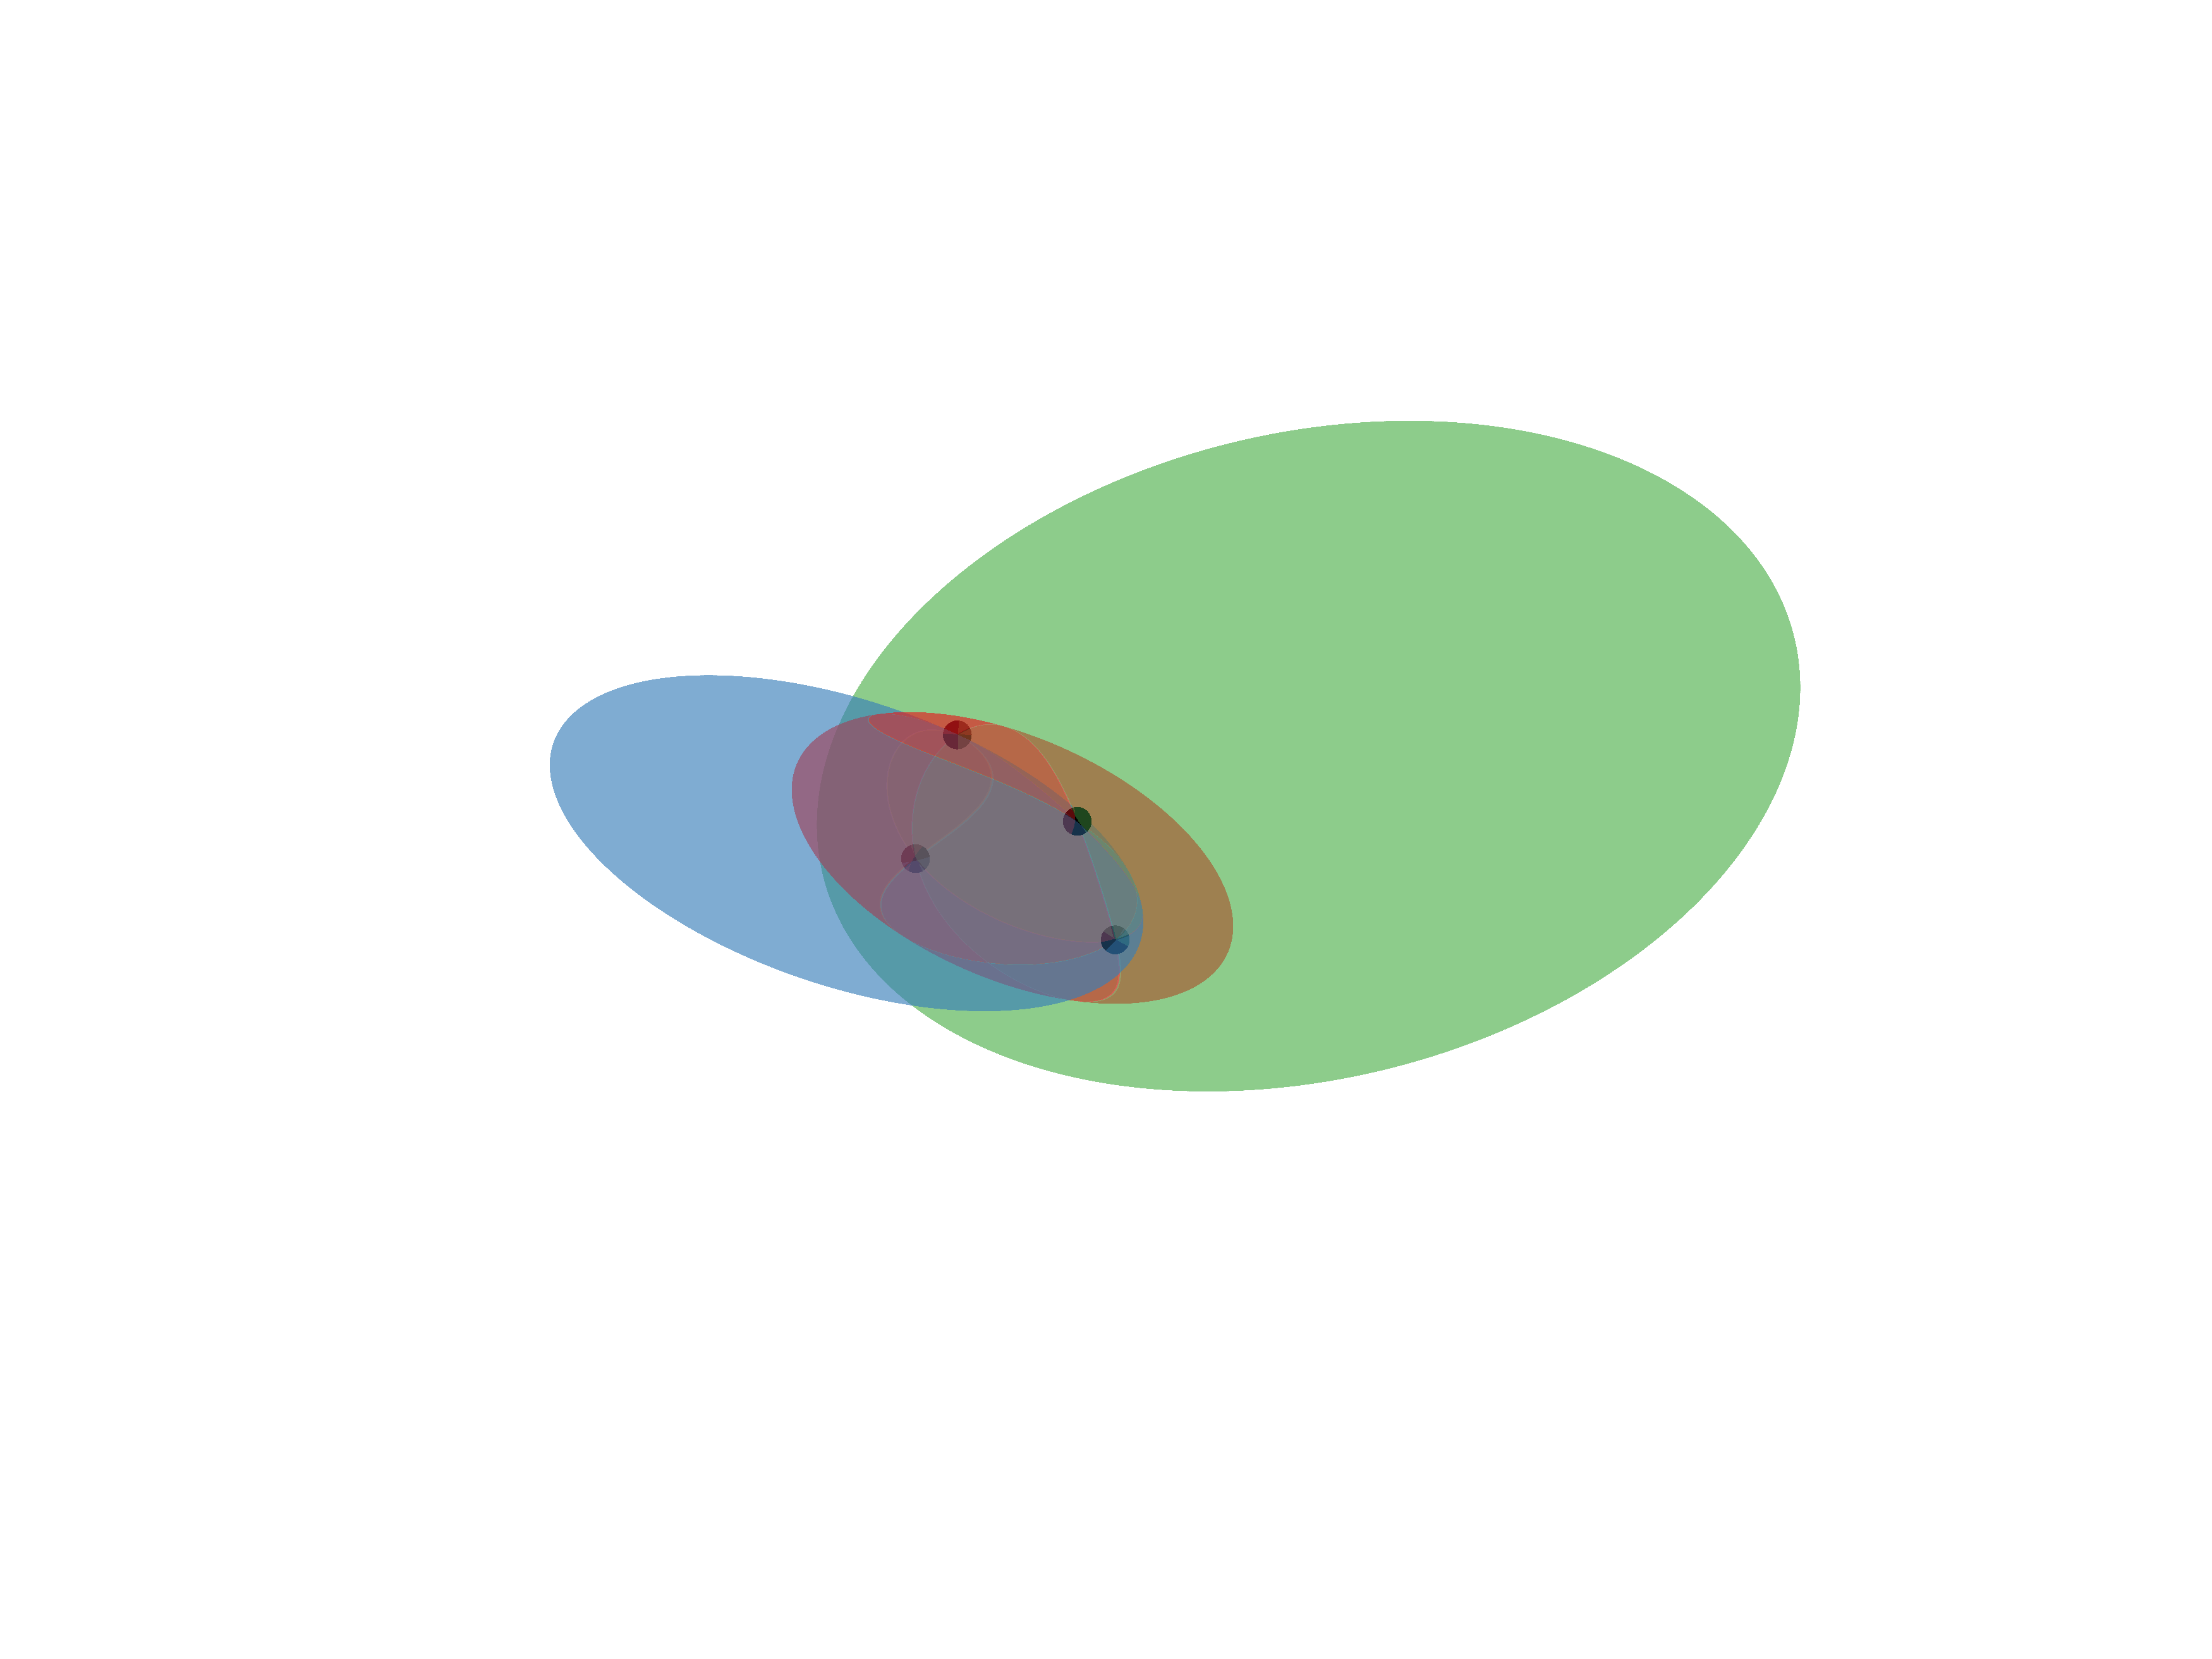
\includegraphics[width=\textwidth]{"images/e3q3_example1.png"}
		 		\subcaption{Die drei Ellipsen aus System \eqref{eqn:example1}}
		 	\end{subfigure}
		 \end{figure}
		 \begin{figure}[H]\ContinuedFloat
			\begin{subfigure}[b]{0.8\textwidth}
				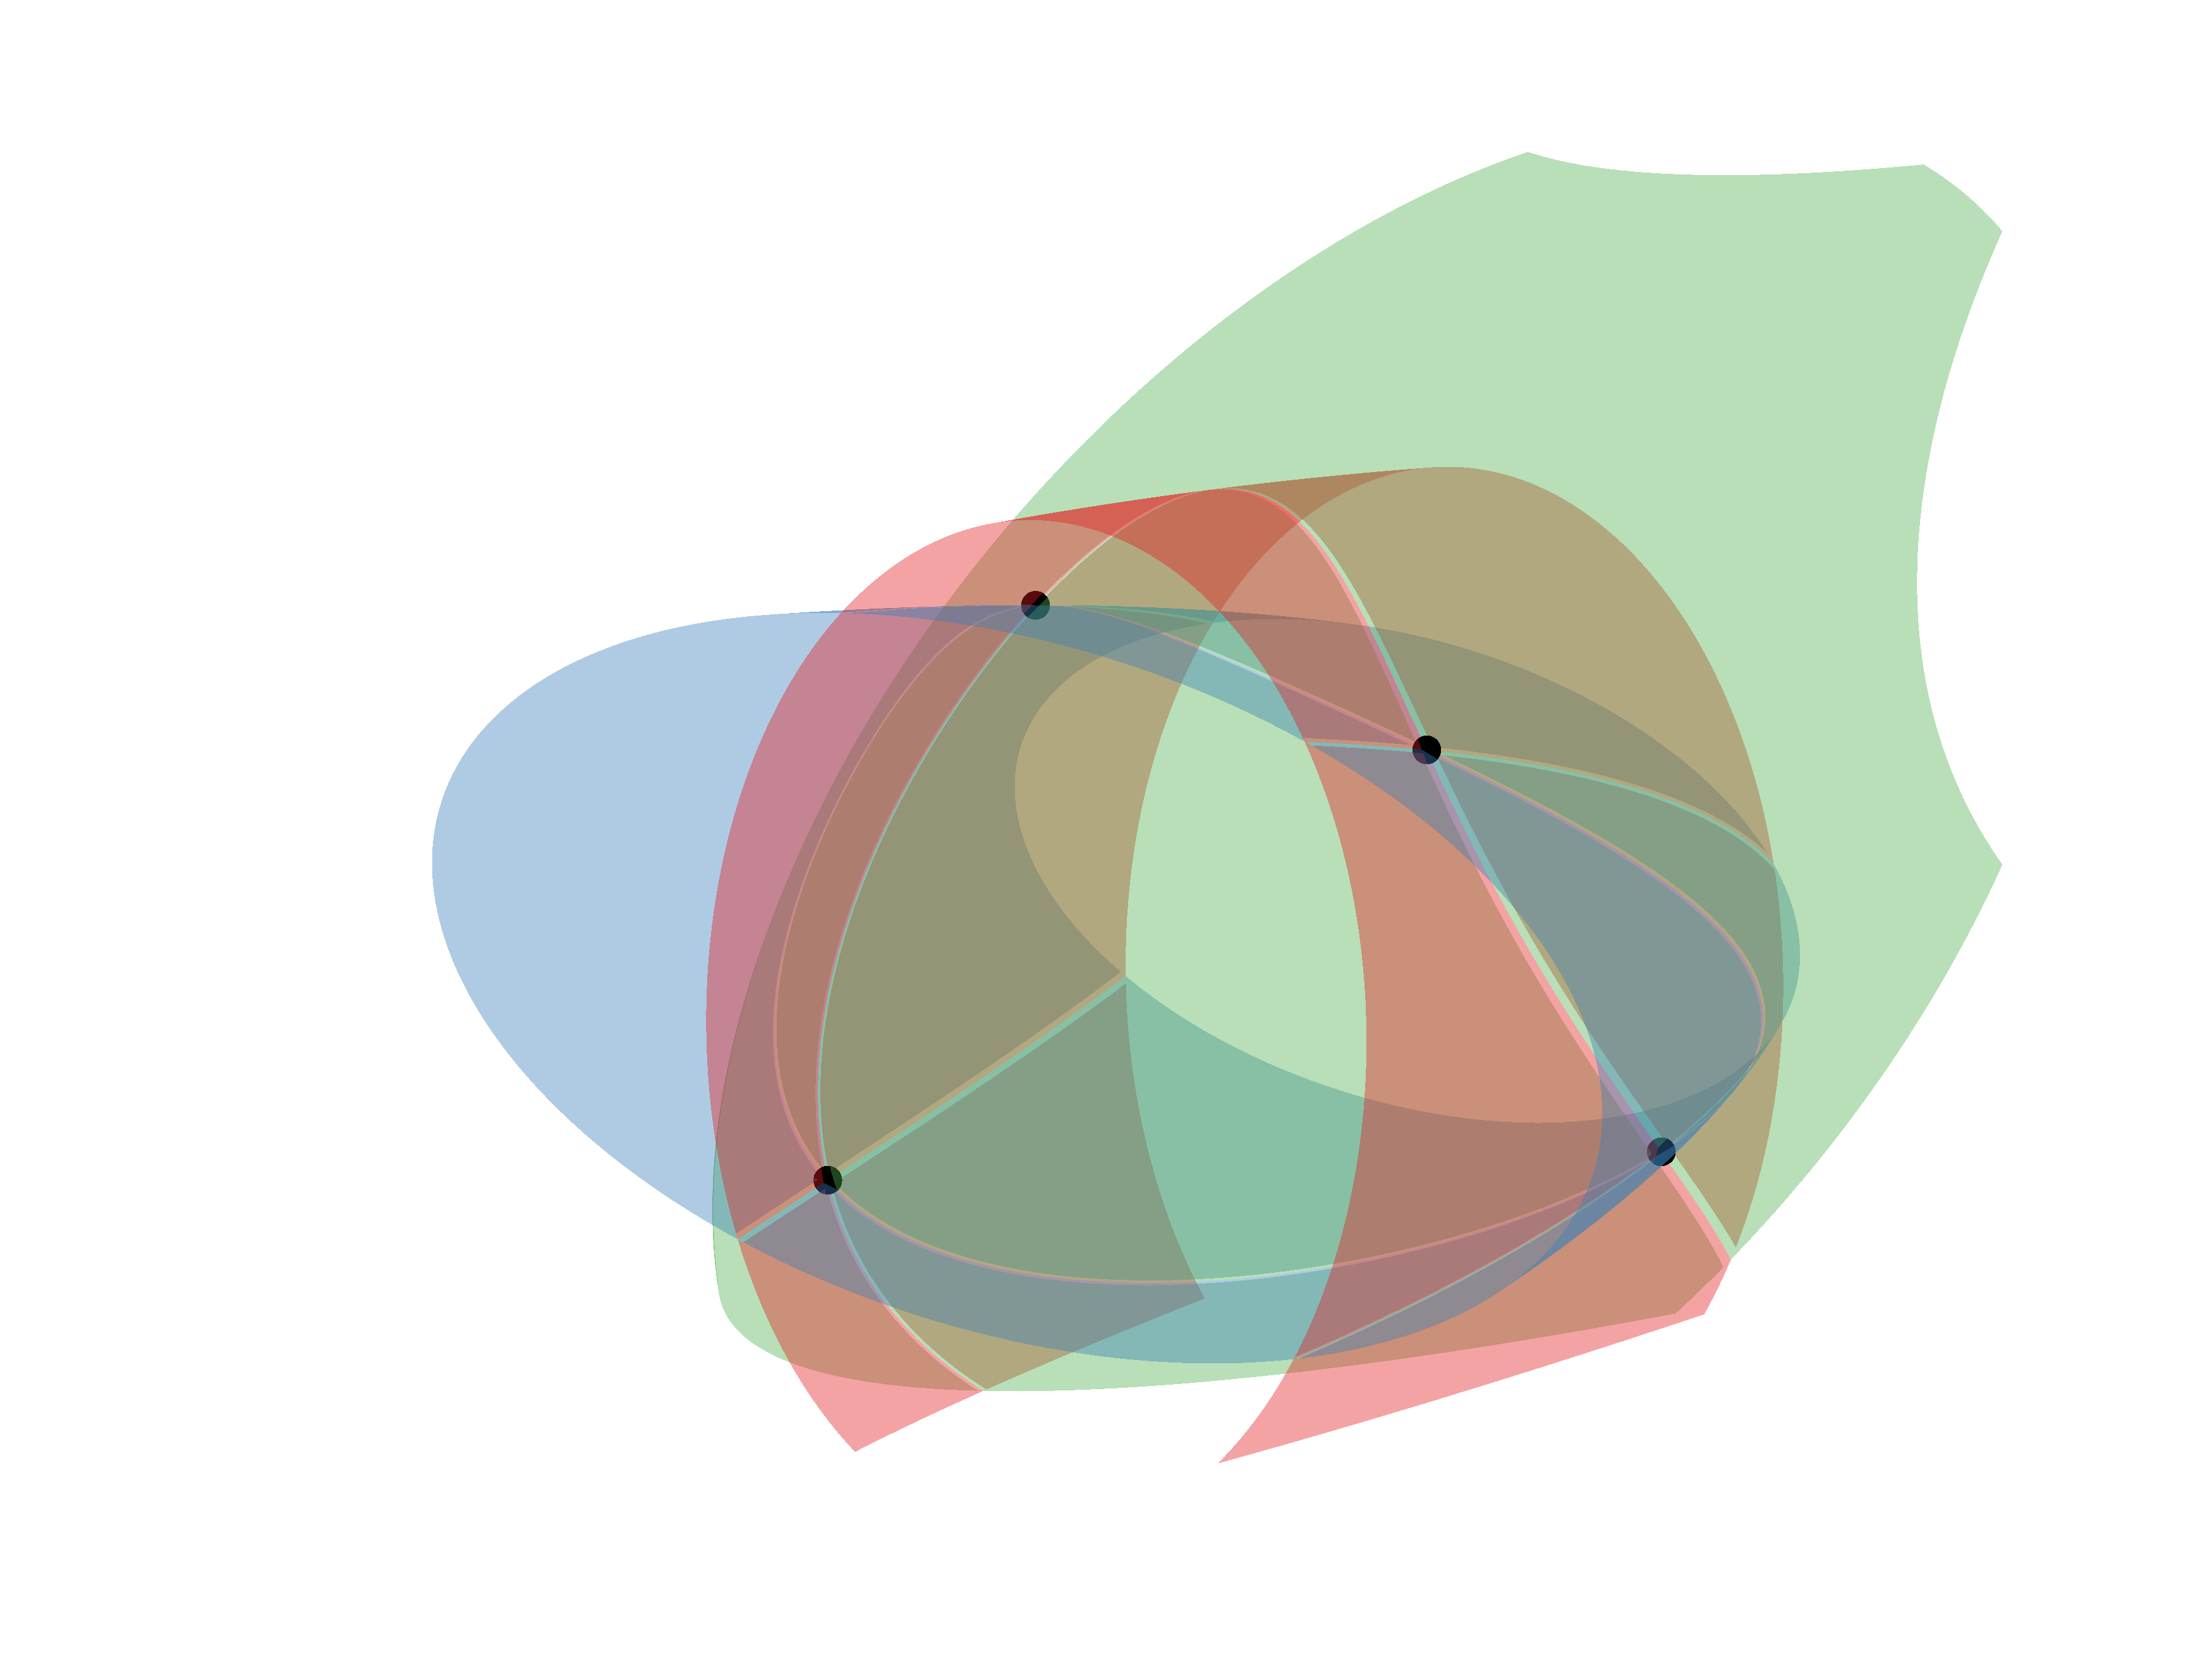
\includegraphics[width=\textwidth]{"images/e3q3_example1_zoom.png"}
				\subcaption{Die Schnittpunkte der drei Ellipsen aus System \eqref{eqn:example1}.}
			\end{subfigure}
			\caption{Geometrie der Quadriken aus Beispiel \eqref{eqn:example1}.}
		 \end{figure}
	
	\begin{example}
		Betrachten wir das System aus Beispiel {\normalfont\ref{ex:3Q3_1}} über $\F{17}$, so erhalten wir das Gleichungssystem
		\begin{equation*}
			\begin{alignedat}{-1}
				     x^2+x\,y+x\,z+x+2\,y^2+y+z^2+z+7&=0,\\
				      x^2+x\,z+7\,x+y^2+16\,y\,z+3\,z^2+7&=0,\\
				       x^2+2\,x+y^2+y\,z+z^2+7&=0.
		\end{alignedat}
		\end{equation*}
		Der Algorithmus findet die Lösungen
		\begin{equation*}
			\begin{alignedat}{5}
				&\left( x_{1},y_{1},z_{1}\right) &=& \left(14,12,10 \right),&&\\
				&\left( x_{2},y_{2},z_{2}\right) &=& \left(7,5,9 \right)&& \quad\text{und} \\
				&\left( x_{3},y_{3},z_{3}\right) &=& \left(16,15,6 \right).&&
			\end{alignedat}
		\end{equation*}
	\end{example}
	\begin{example}
		Das Gleichungssystem
		\begin{equation*}\label{eqn:example3}
			\begin{alignedat}{-1}
				x^2+5\,y^2-50\,y-20\,z+9&=0,\\
				 -x^2+2\,x\,y-11\,x+y^2-18\,y+5\,z+\frac{187}{2}&=0,\\ 2\,x^2-x\,y-3\,x+13\,y^2+2\,y\,z-200\,y+4\,z^2+12\,z+826&=0
			\end{alignedat}
		\end{equation*}
		besitzt über $\R$ die Lösungen
		\begin{equation*}
			\begin{alignedat}{5}
				&\left( x_{1},y_{1},z_{1}\right) &=& \left(1,8,-3.5 \right)&& \quad\text{und} \\
				&\left( x_{2},y_{2},z_{2}\right) &=& \left(4.13496,7.72621,-3.08705 \right).&&
			\end{alignedat}
		\end{equation*}
		\begin{figure}[H]
			\centering
			\begin{subfigure}[b]{0.8\textwidth}
				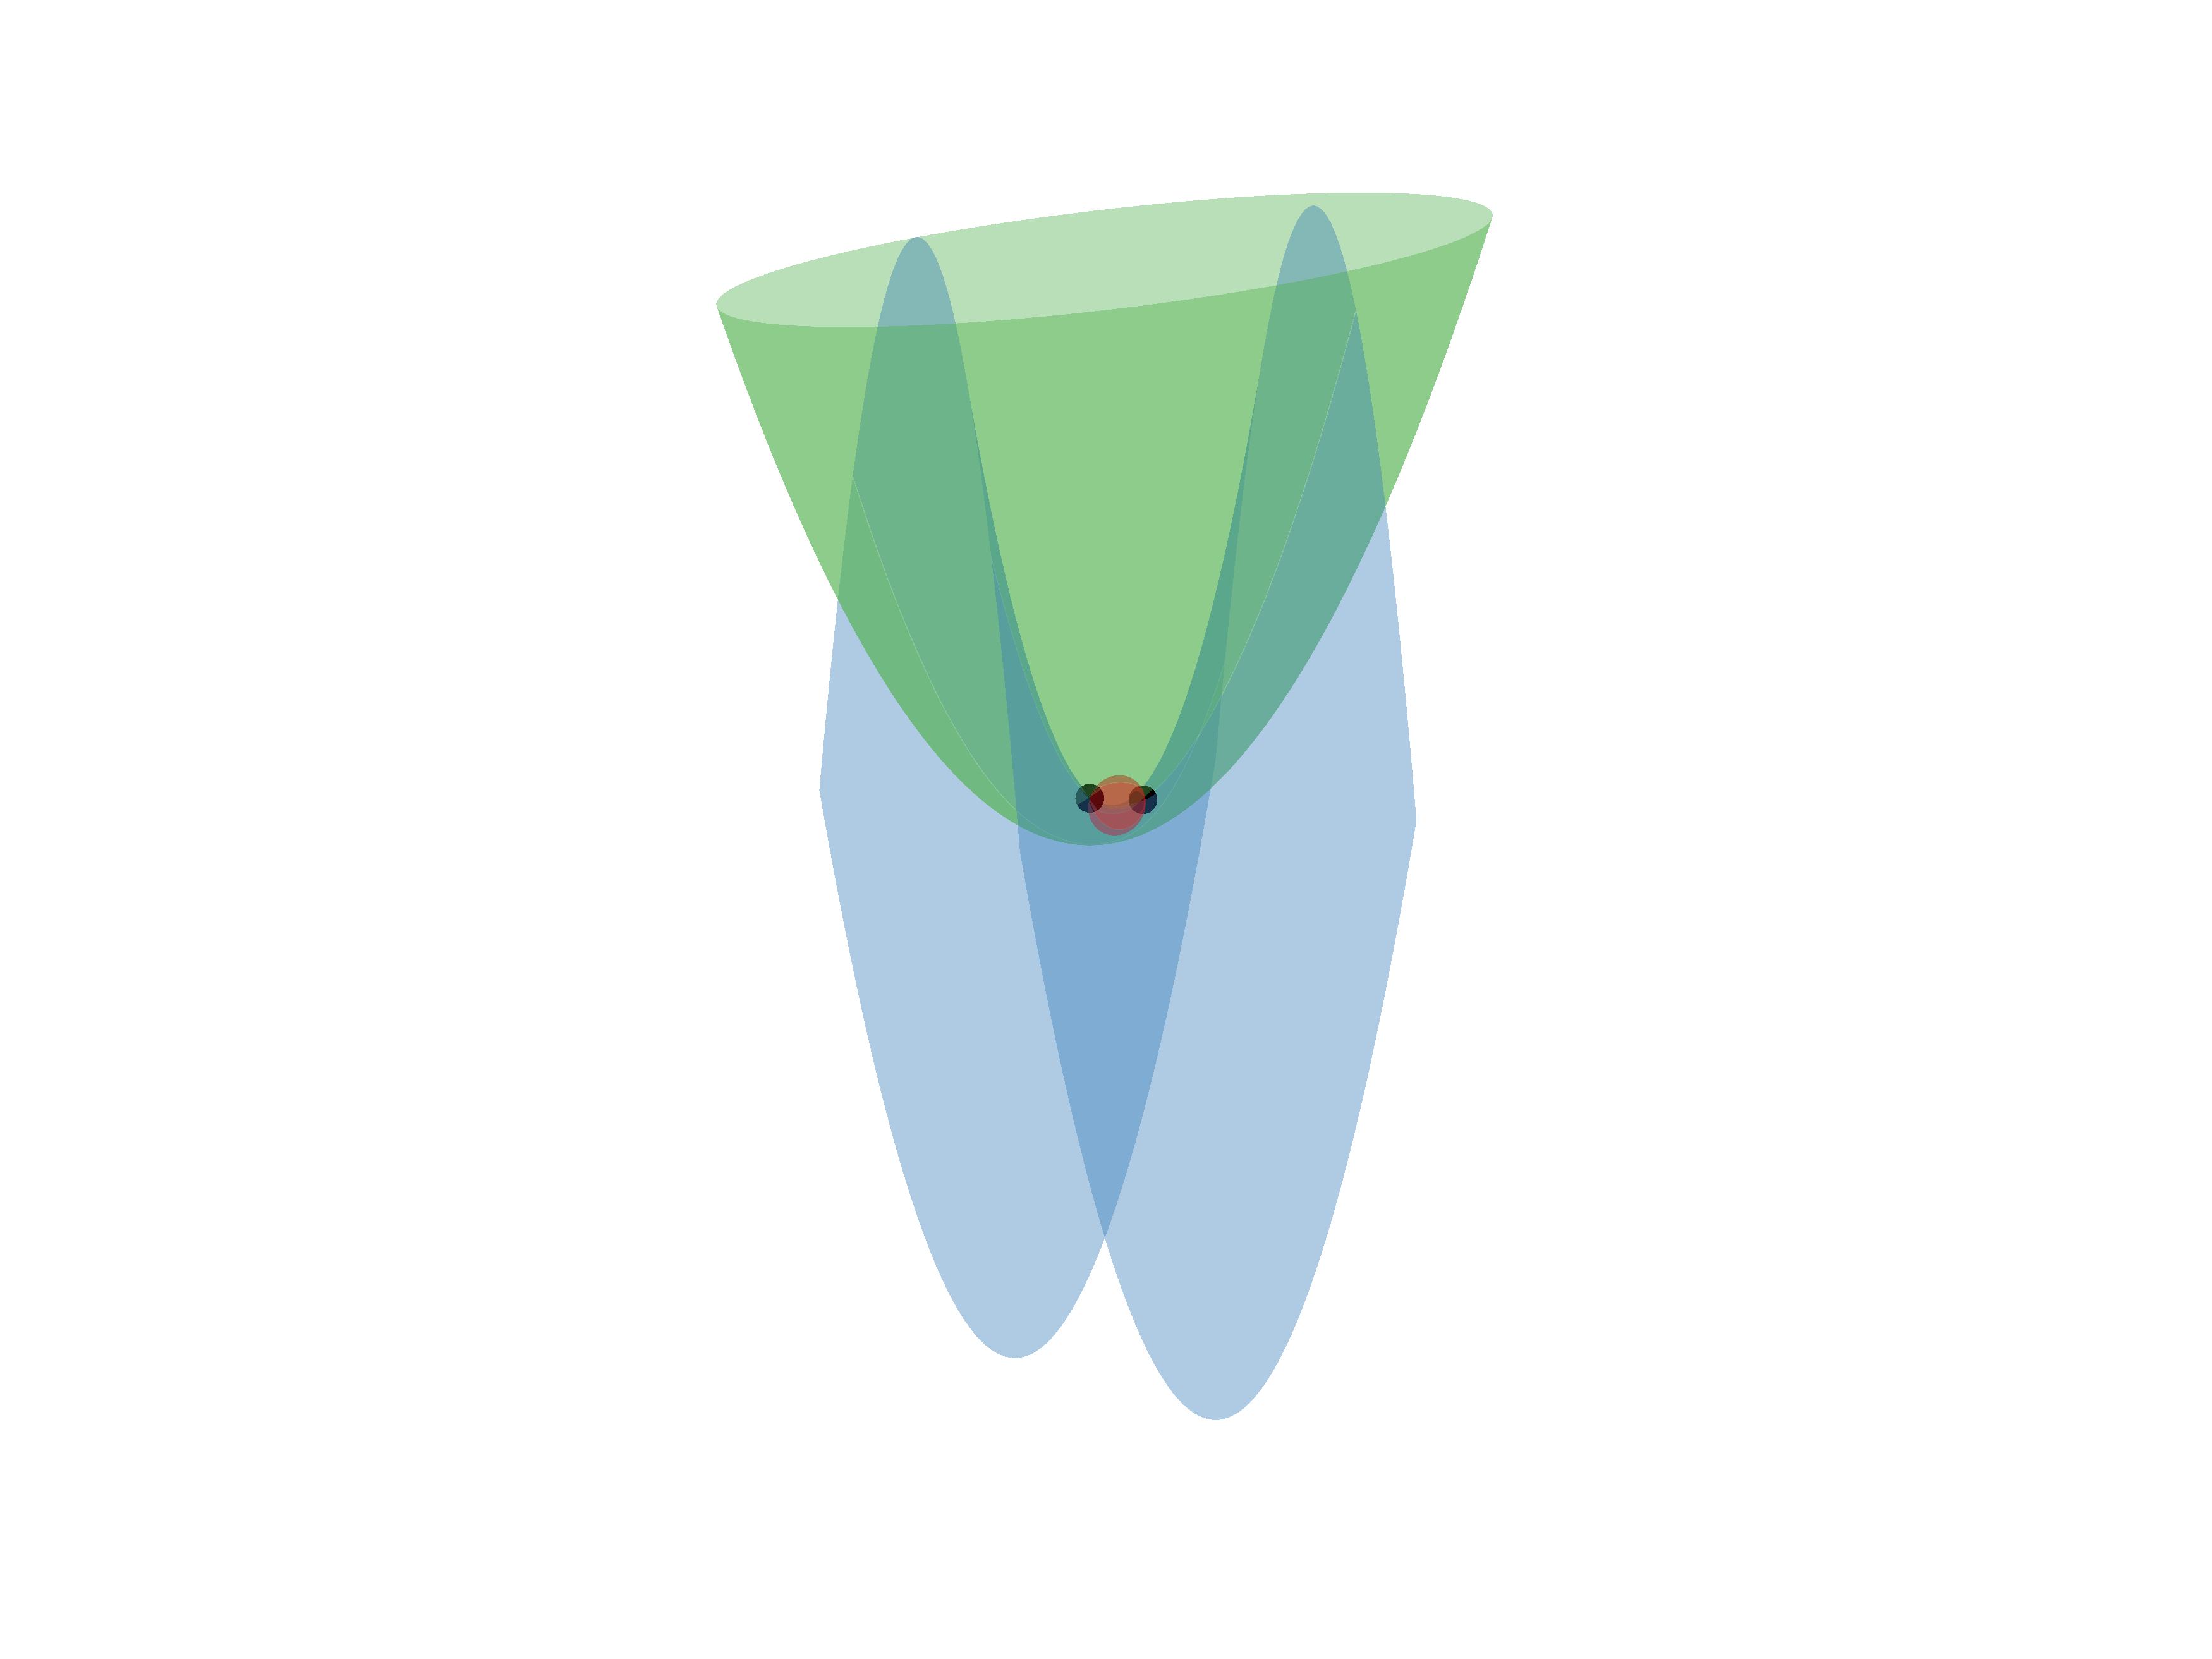
\includegraphics[width=\textwidth]{"images/e3q3_example2.png"}
				\subcaption{Die Ellipse, der elliptische und hyperbolische Paraboloid aus System \eqref{eqn:example3}.}
			\end{subfigure}
		\end{figure}
					\begin{figure}[H]\ContinuedFloat
			\begin{subfigure}[b]{0.8\textwidth}
				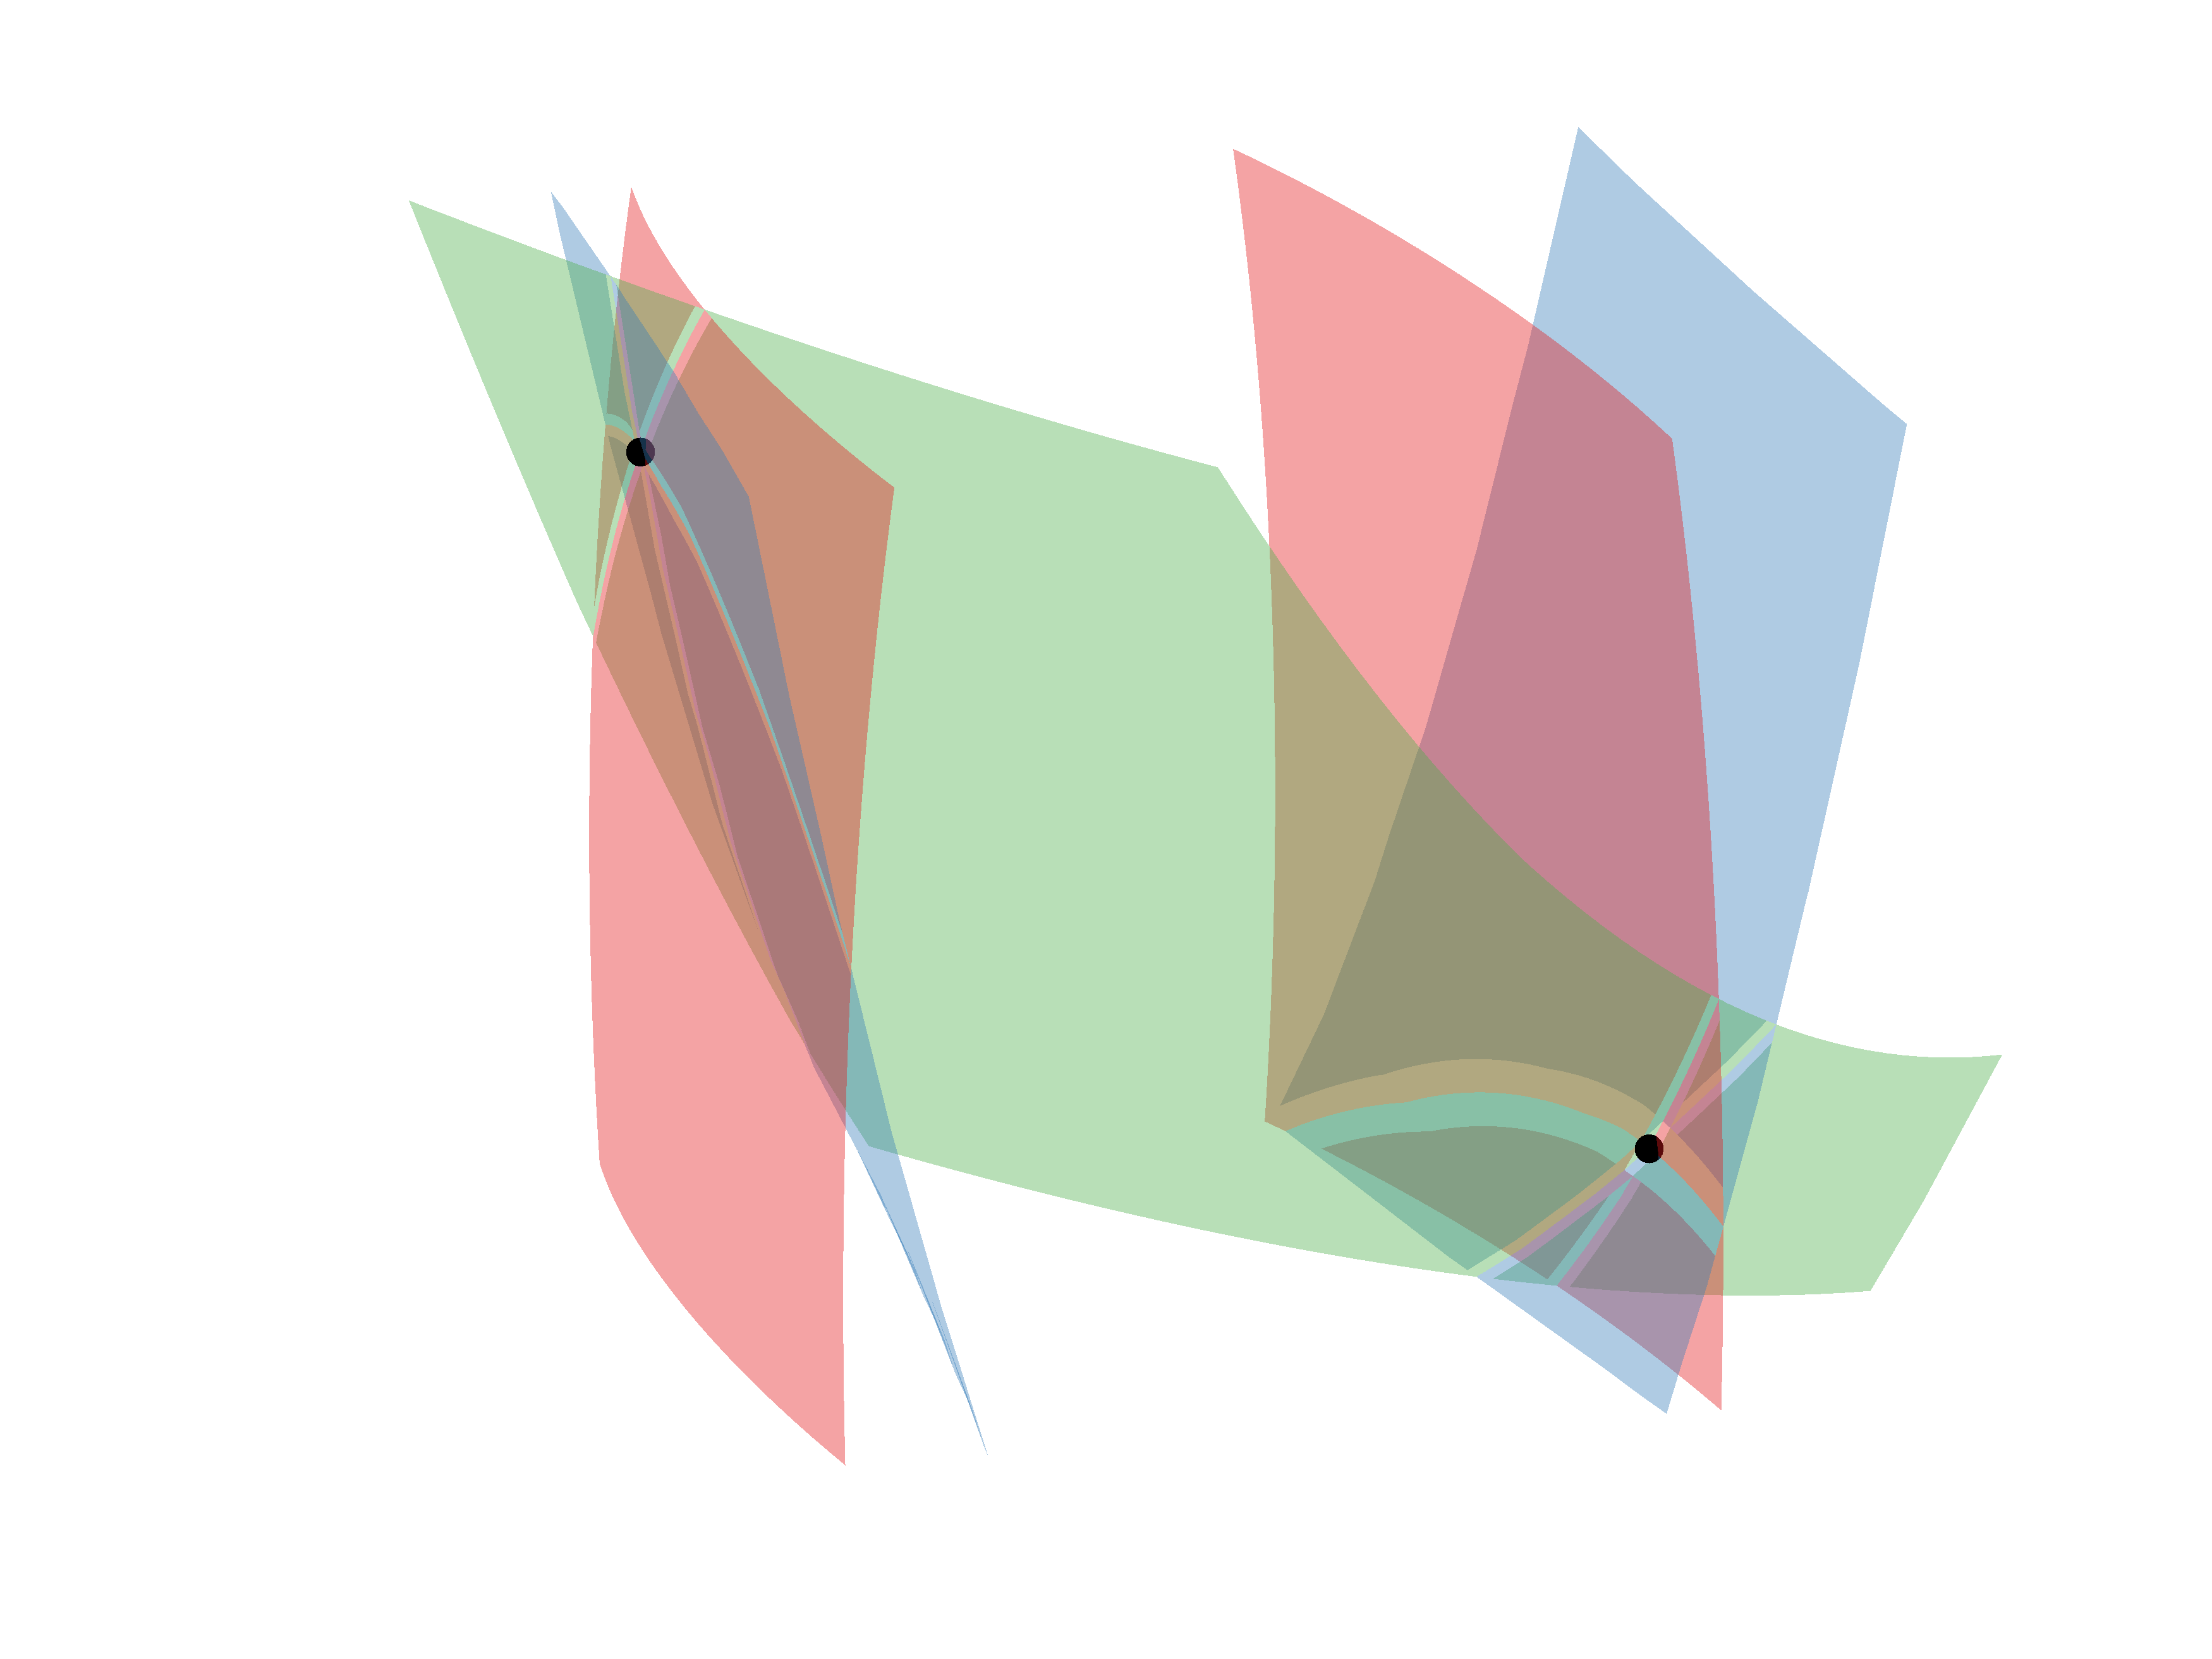
\includegraphics[width=\textwidth]{"images/e3q3_example2_zoom.png"}
				\subcaption{Die Schnittpunkte der drei Quadriken aus System \eqref{eqn:example3}.}
			\end{subfigure}
			\caption{Globale und lokale Geometrie der Quadriken über $\R$.}
		\end{figure}
	\end{example}
	\newpage
		\begin{example}
		Gegeben sei das Gleichungssystem

			\begin{equation*}
				\begin{alignedat}{-1}
					29236\,x^2+5262\,x+13670\,y+29511\,z+52080\,y\,z-5044&=0,\\ -6089\,x+6437\,y-3619\,z+9520\,x\,z+16456\,y\,z+36592\,z^2+20861&=0,\\ 40362\,y^2+18928\,y+17093\,x+1294\,z+29534&=0
				\end{alignedat}
			\end{equation*}

		über $\F{69427}$.
		So findet der Algorithmus  die Lösungen
		\begin{equation*}\label{eqn:example4}
			\begin{alignedat}{5}
				&\left( x_{1},y_{1},z_{1}\right) &=& \left(44102,315,37257 \right),&& \\
				&\left( x_{2},y_{2},z_{2}\right) &=& \left(28952,50009,7 \right),&& \\
				&\left( x_{3},y_{3},z_{3}\right) &=& \left(41633,37973,37946 \right)&& \quad\text{und} \\
				&\left( x_{4},y_{4},z_{4}\right) &=& \left(59854,61171,7135 \right).&&
			\end{alignedat}
		\end{equation*}
	\end{example}
	\begin{example}
		Gegeben sei das Gleichungssystem
		
		\begin{equation*}\label{eqn:example5}
			\begin{alignedat}{-1}
				x^2+3\,y^2+y\,z+z^2-5&=0,\\
				 3\,x^2+2\,y^2+2\,y\,z+z^2-5&=0,\\
				2\,x^2+y^2-y\,z+2\,z^2-5&=0
			\end{alignedat}
		\end{equation*}
		
		über $\R$.
		Der Algorithmus findet die Lösungen
		\begin{equation*}
			\begin{alignedat}{5}
				&\left( x_{1},y_{1},z_{1}\right) &=& \left(-1.0351,1.19523,-0.597614 \right),&& \\
				&\left( x_{2},y_{2},z_{2}\right) &=& \left(-1.0351,-1.19523,0.597614\right),&& \\
				&\left( x_{3},y_{3},z_{3}\right) &=& \left(1.0351,1.19523,-0.597614 \right),&& \quad\text{und} \\
				&\left( x_{4},y_{4},z_{4}\right) &=& \left(1.0351,-1.19523,0.597614 \right).&&
			\end{alignedat}
		\end{equation*}
	\end{example}
		\begin{figure}[H]
			\centering
			\begin{subfigure}[b]{0.8\textwidth}
				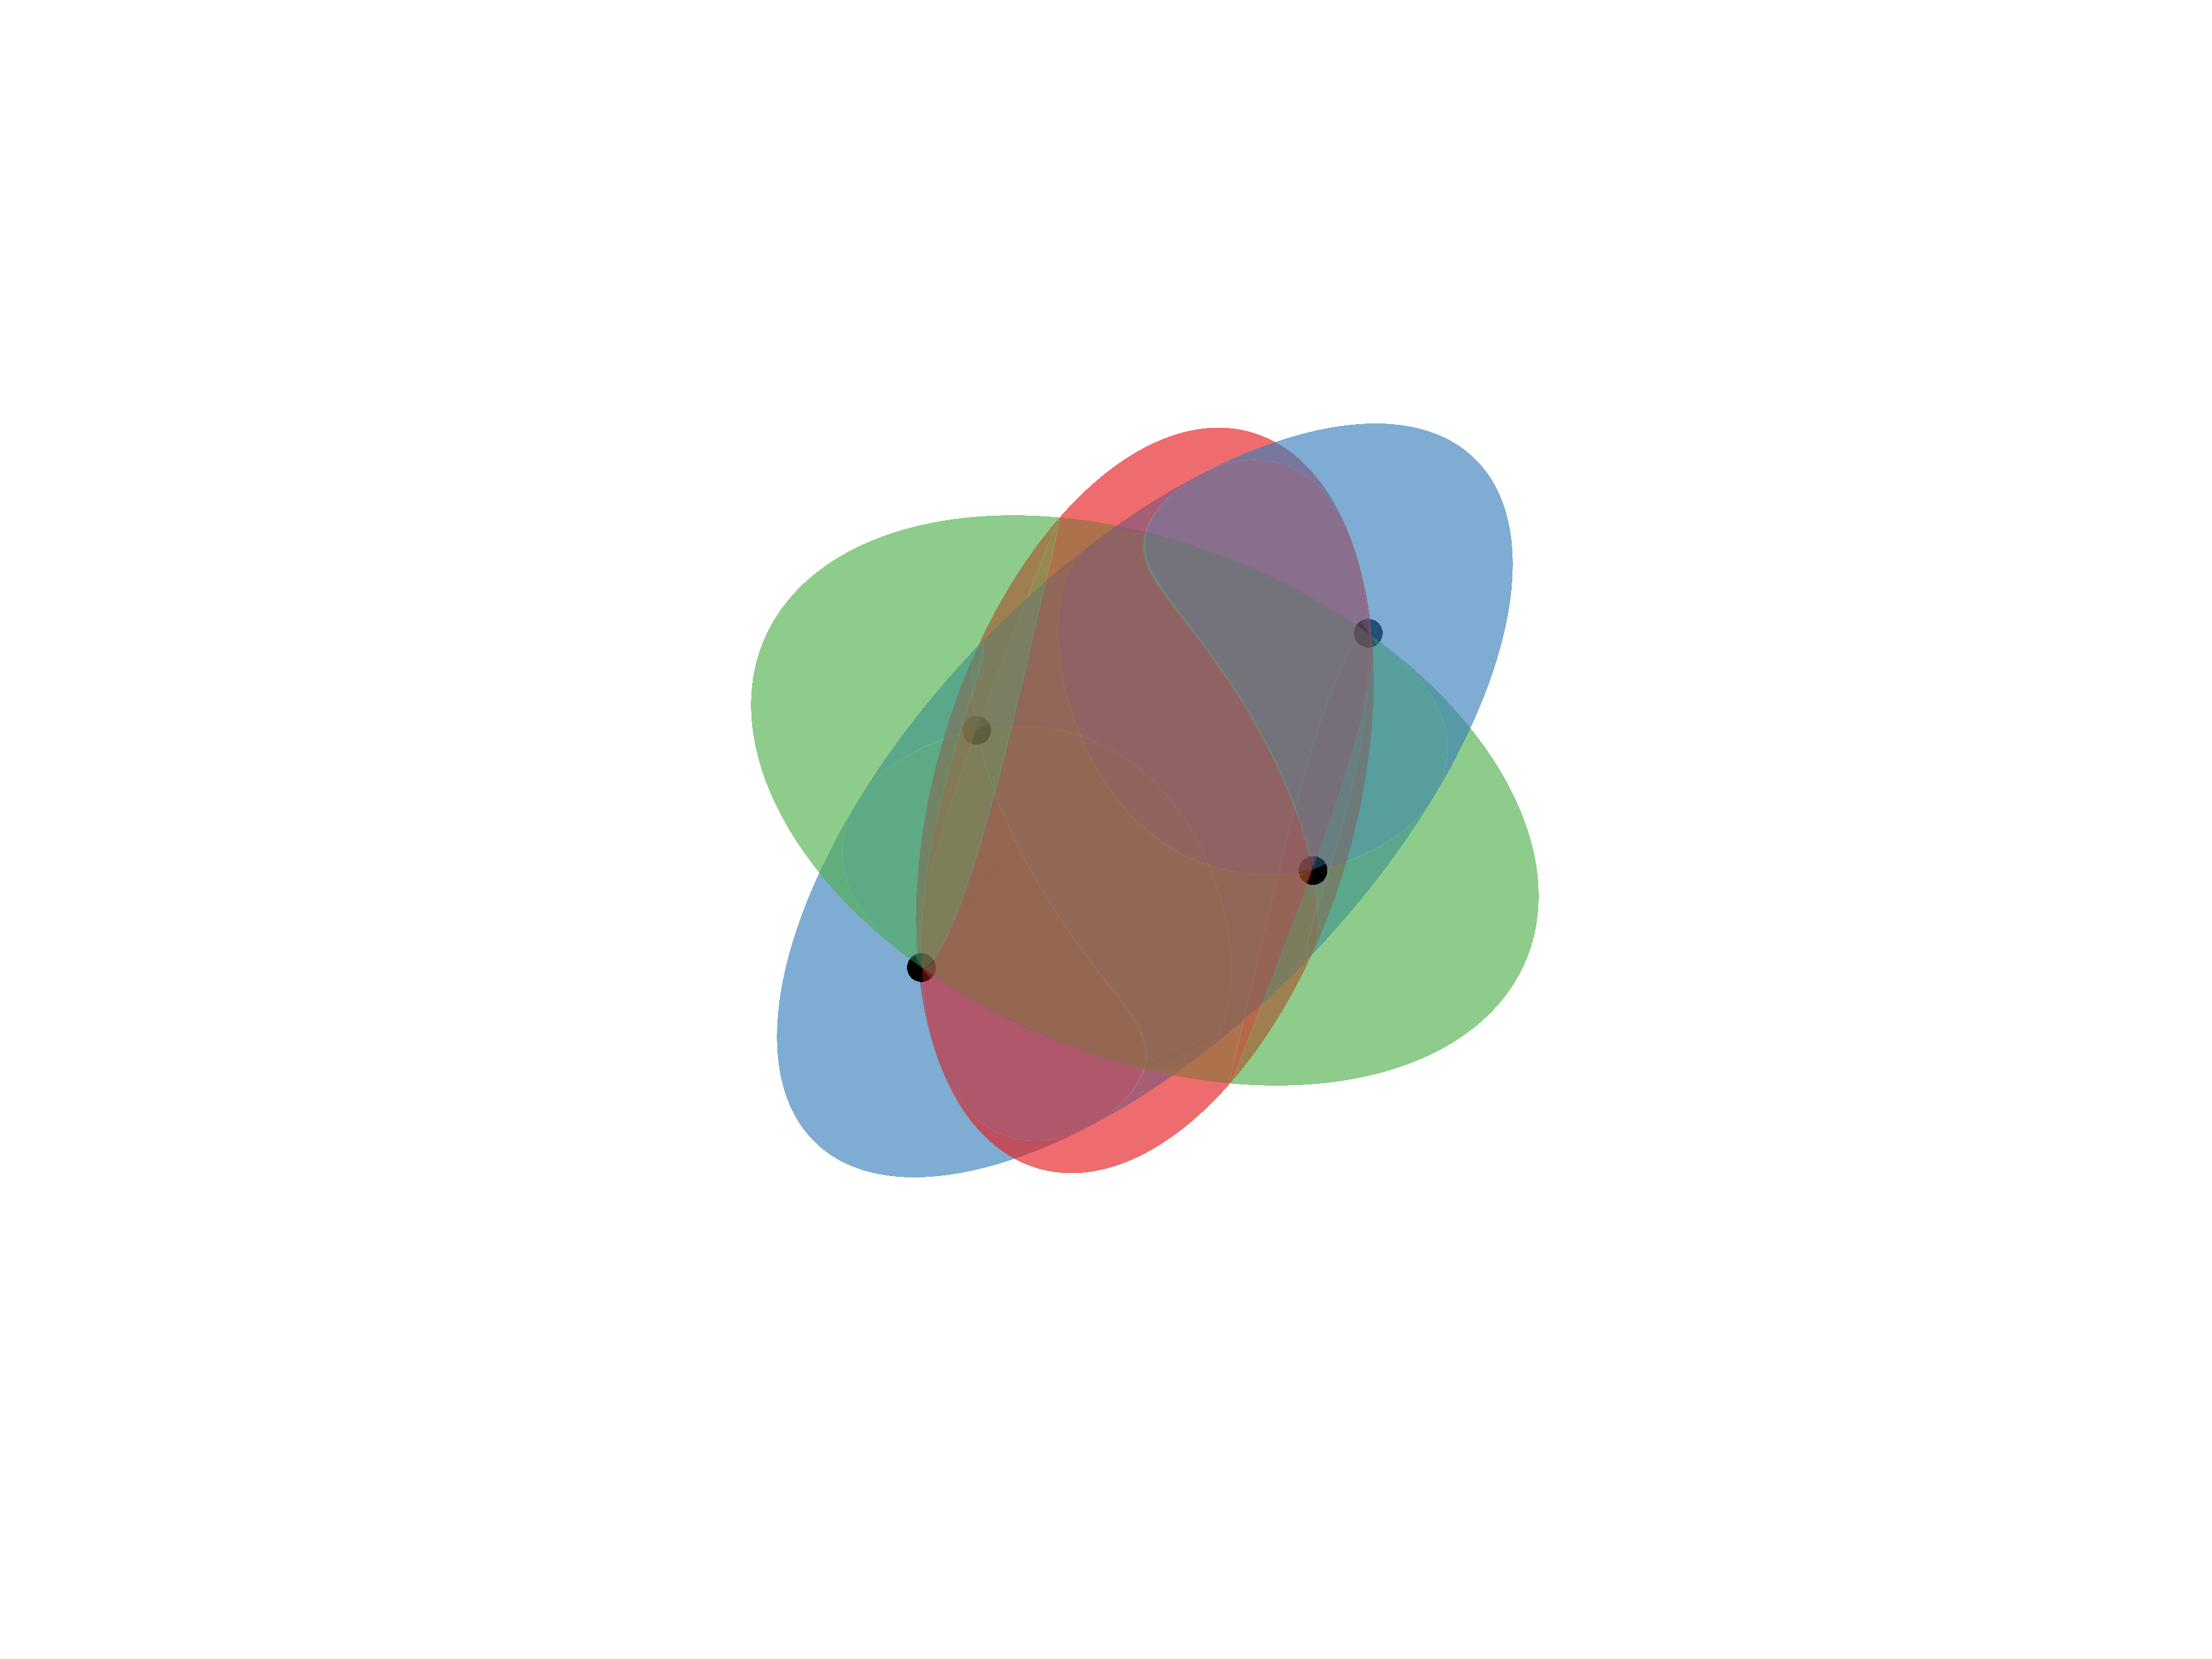
\includegraphics[width=\textwidth]{"images/e3q3_example3.png"}
				\subcaption{Die drei Ellipsen aus System \eqref{eqn:example5}.}
			\end{subfigure}
		\end{figure}
		\begin{figure}[H]\ContinuedFloat
			\begin{subfigure}[b]{0.8\textwidth}
				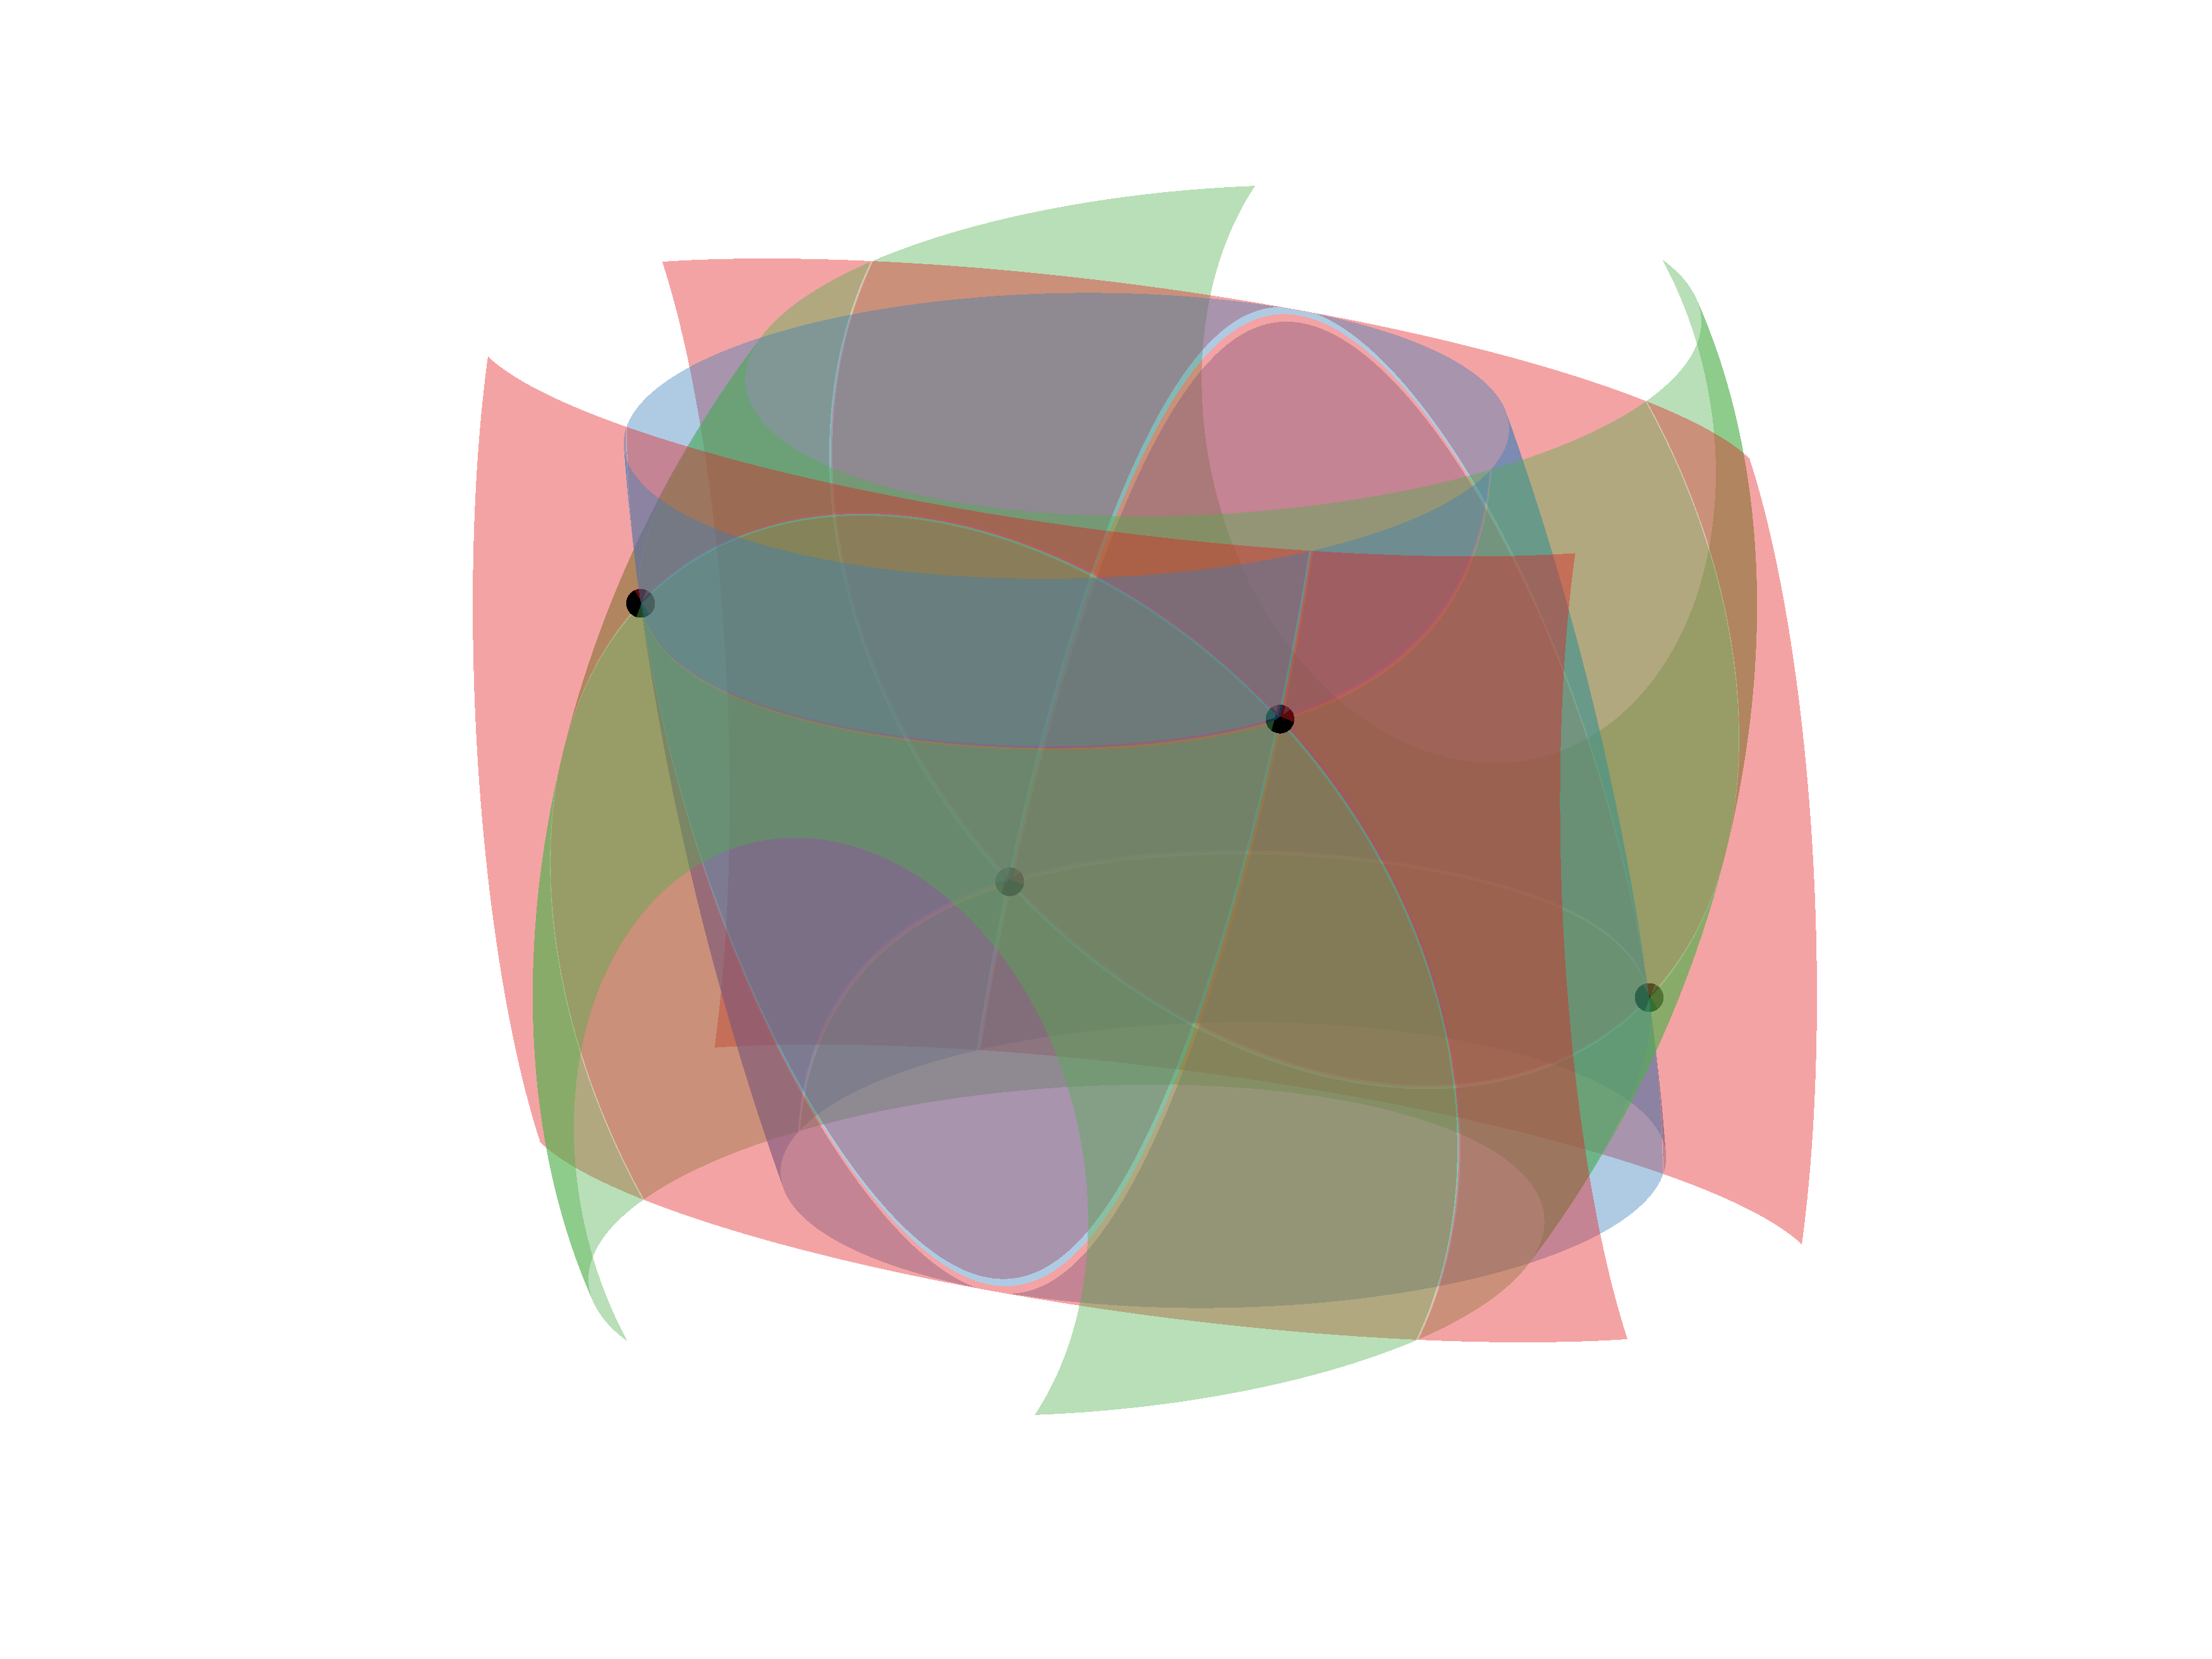
\includegraphics[width=\textwidth]{"images/e3q3_example3_zoom.png"}
				\subcaption{Die Schnittpunkte der drei Quadriken aus System \eqref{eqn:example5}.}
			\end{subfigure}
		\end{figure}
		\begin{figure}[H]\ContinuedFloat
			\begin{subfigure}[b]{0.8\textwidth}
				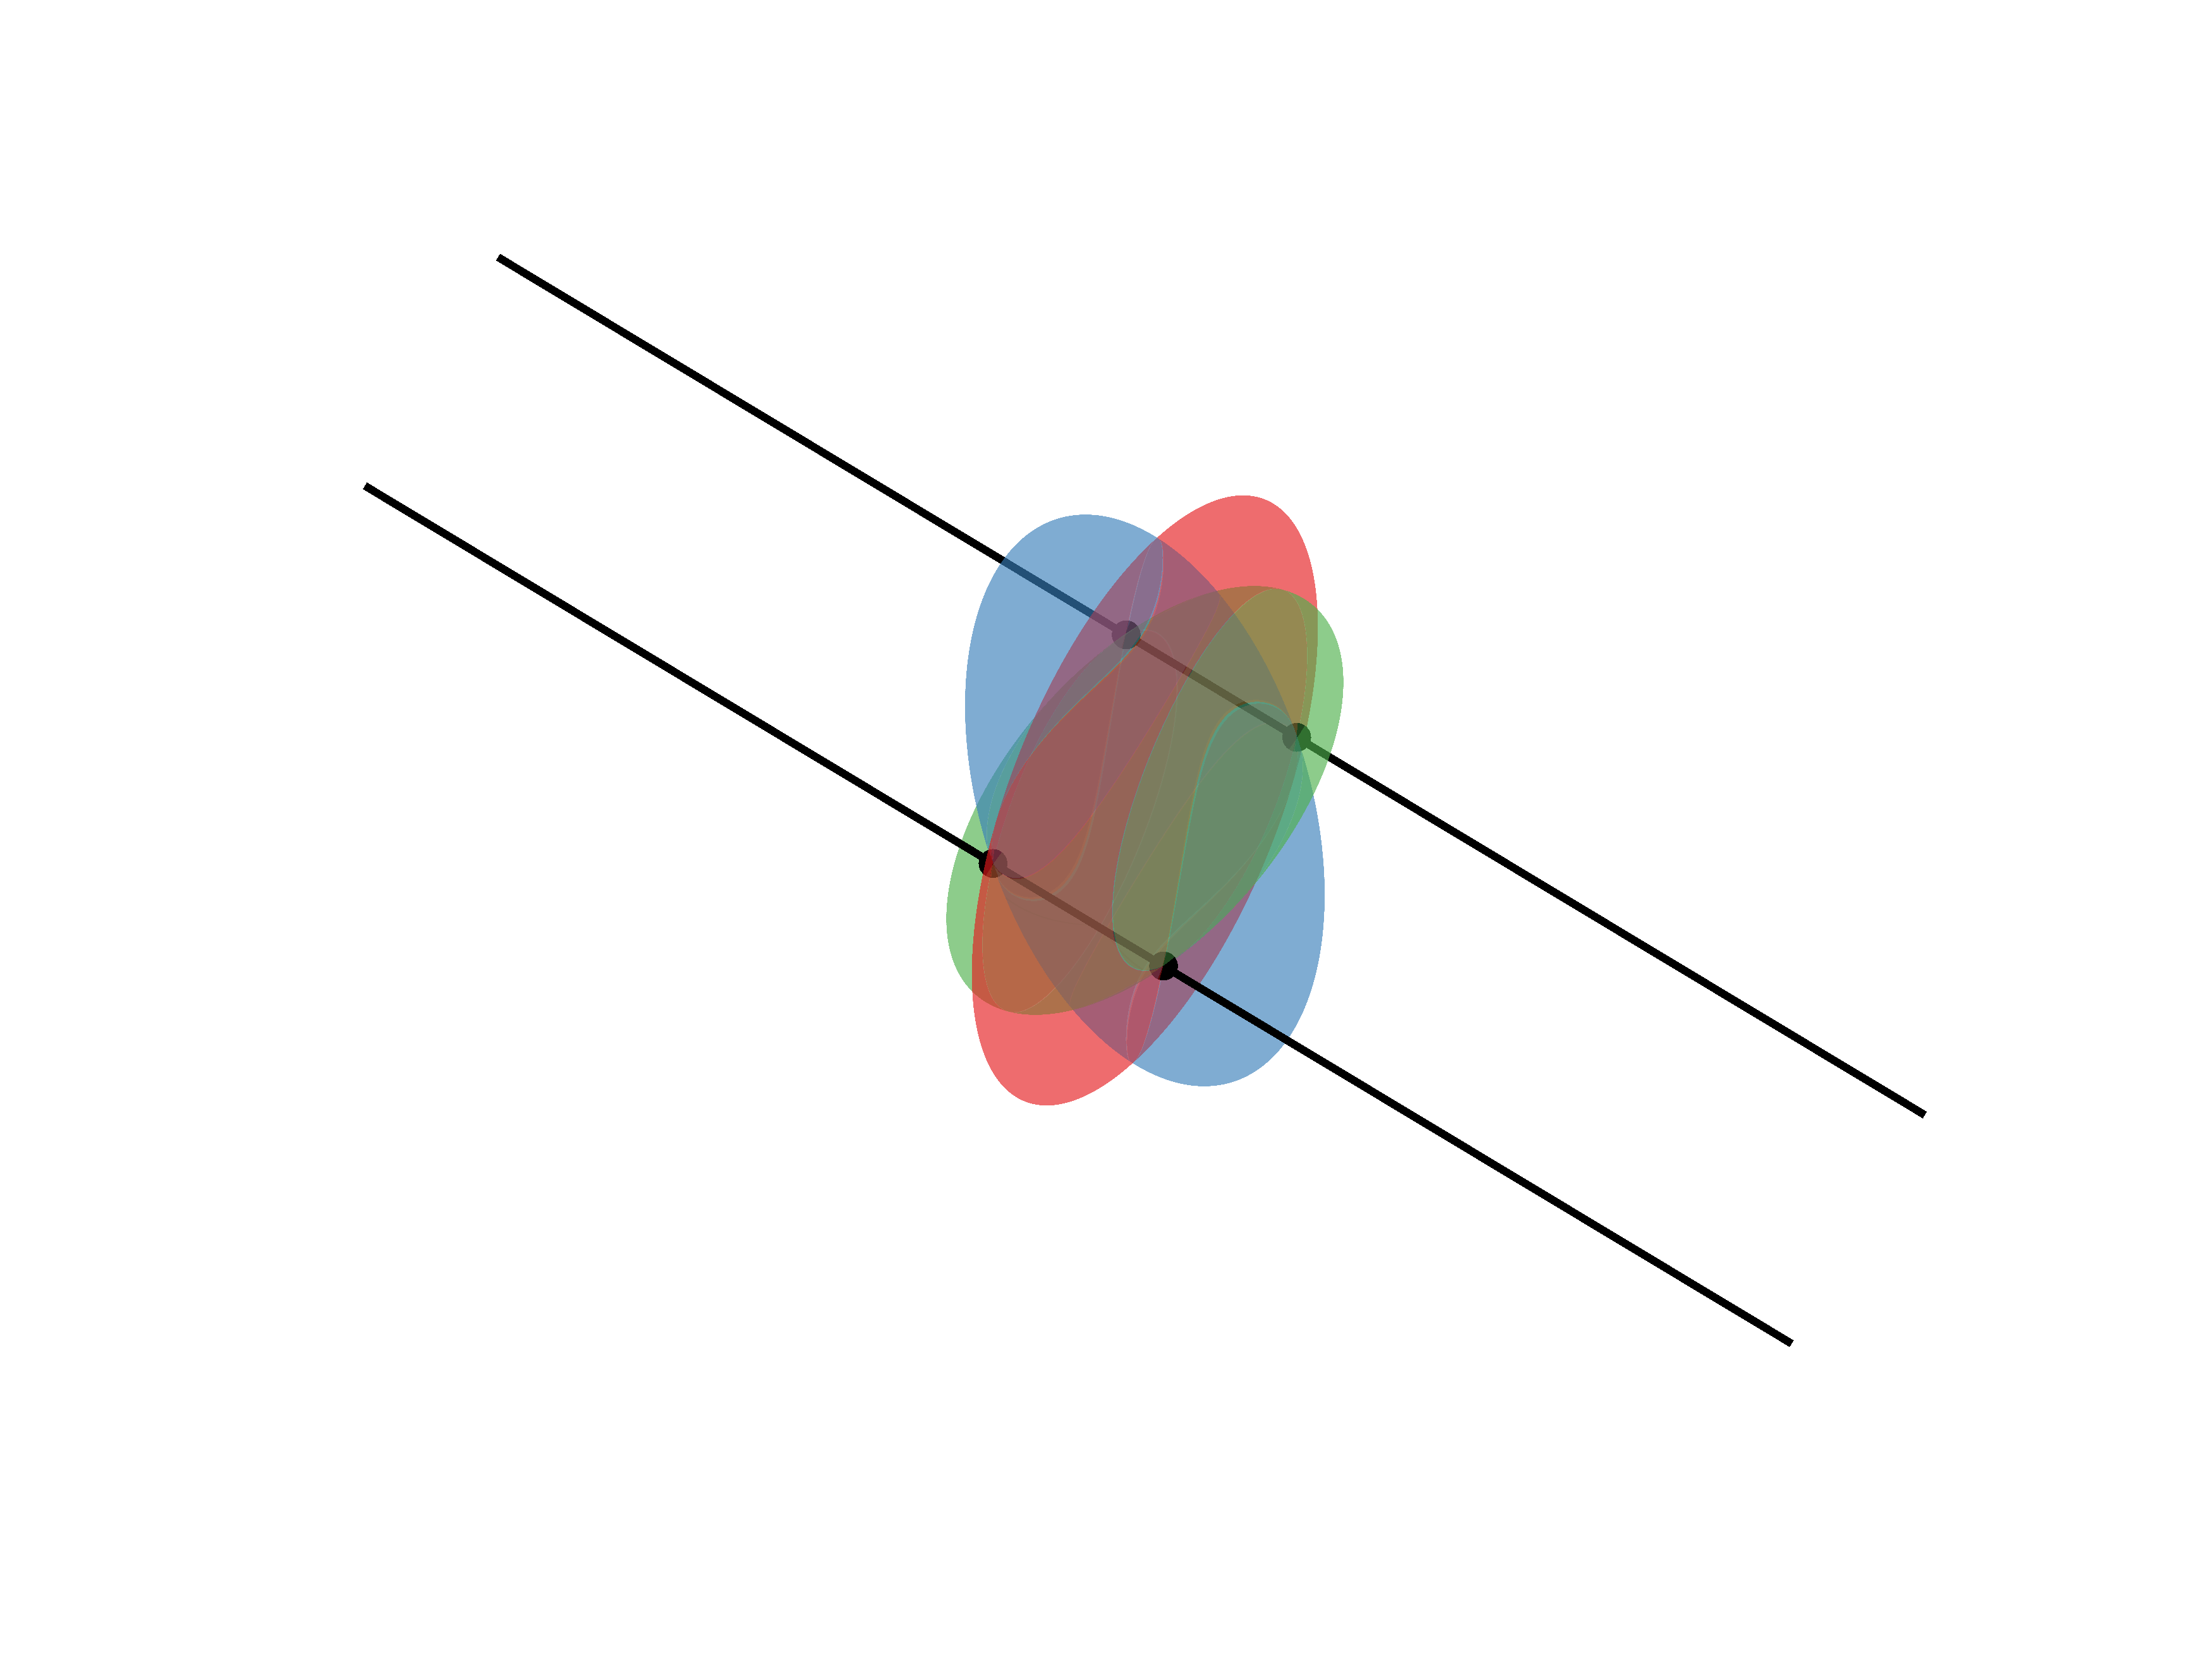
\includegraphics[width=\textwidth]{"images/e3q3_example3_lines.png"}
				\subcaption{Die Geraden nach Gleichung \eqref{eqn:3Q3_r1} zwischen den Schnittpunkten aus System \eqref{eqn:example5}.}
			\end{subfigure}
			\caption{Drei Ellipsoide mit dem gleichen Zentrum aber unterschiedlichen Hauptachsen und Rotationen.}
		\end{figure}
	
	\newpage
\section{Verallgemeinerung auf kubische Flächen}\label{chp:5C3}
\subsection{Verallgemeinerte Fassung des E3Q3-Algorithmus}\label{sec:mC3}
Um das Vorgehen des E3Q3-Algorithmus auf Gleichungssysteme kubischer Hyperflächen zu übertragen formulieren wir analog zuerst das allgemeine mC3-Problem.

\begin{definition}[$mC3$-Problem]\label{def:mC3}
	Sei $K$ ein Körper und seien $X_1$,$X_{2}$ und $X_{3}$ die Unbestimmten unseres Gleichungssystems. Weiter seien $m \in \N$ und $C \in K^{m\times 20}$ bezeichne die Koeffizientenmatrix. Das Gleichungssystem, welches es zu lösen gilt, lautet dann
	\begin{gather}\label{eqn:mC3}
		\begin{alignedat}{5}
			& c_{1} \cdot &v&,
			&=&0\\
			& c_{2} \cdot &v&,
			&=&0\\
			&&\vdots&&&\\
			& c_{m} \cdot &v&
			&=&0,
		\end{alignedat}
	\end{gather}
	wobei $c_{i}$ für die $i$-te Zeile der Matrix $C$ und $v$ für den Monomvektor 

\begin{equation*}
v = 	
	\begin{pmatrix}
			   X_{1}^3,X_{1}^2X_{2},X_{1}^2X_{3},X_{1}X_{2}^2,X_{1}X_{2}X_{3},X_{1}X_{3}^2,X_{2}^3,X_{3}^3,X_{2}^2X_{3},\ldots \\
		  X_{2}X_{3}^2,X_{1}^2,X_{1}X_{2},X_{1}X_{3},X_{2}^2,X_{2}X_{3},X_{3}^2,X_{1},X_{2},X_{3},1
\end{pmatrix}
^{\top} \in K[X_1,X_2,X_3]^{20}
\end{equation*}

	steht.
\end{definition}
Analog zu dem Vorgehen in Abschnitt \ref{sec:E3Q3} betrachten wir $m$ Gleichungen in $K\left[ X_{1}\right] \left[X_{2},X_{3}\right] $ anstatt in $K\left[ X_{1},X_{2},X_{3}\right]$. Wir nehmen $X_{1}$ also zuerst in den Koeffizientenring auf und unterteilen die verbleibenden Monome in den Unbestimmten $X_{2},\ X_{3}$ auf zwei Gruppen.
Dies führt zu den 10 Kandidaten 
\begin{equation}
	\{X_{2}^3,X_{2}^2X_{3},X_{2}X_{3}^2,X_{3}^3,X_{2}^2,X_{2}X_{3},X_{3}^2,X_{2},X_{3},1\},
\end{equation}
welche wir nun in die zwei Gruppen 
\begin{equation}\label{eqn:mC3grp}
	\begin{alignedat}{1}
	G_1 &\coloneqq \{\mu_1,\ldots,\mu_n\} \ \text{und} \\
	G_2 &\coloneqq \{\eta_1,\ldots,\eta_{o}\}
\end{alignedat}
\end{equation}
mit $o\coloneqq 10 - n$ aufteilen wollen.

Für diese Aufteilung ergibt sich das Gleichungssystem in Matrixform als
\begin{equation}
	-A \cdot \left(\mu_1,\ldots,\mu_n\right)^{\top} = P \cdot \left(\eta_1,\ldots,\eta_{o}\right)^{\top},
\end{equation}
mit den Matrizen $A \in K[X_1]^{m \times n}$ und $P \in K[X_1]^{m \times o}$.\\
Im nächsten Schritt isolieren wir die $\mu_k$'s, indem wir beide Seiten mit der inversen Matrix zu $A$ multiplizieren.

Für $m = n$ erhalten wir also 
\begin{equation}\label{eqn:cub_inv_eqs}
	\left(\mu_1,\ldots,\mu_n\right)^{\top} = -A^{-1} P \cdot \left(\eta_1,\ldots,\eta_{o}\right)^{\top},
\end{equation}
mit $A \in K^{n \times m}$ und $P \in K[X_1]^{m \times o}$
und können mit dem Substitutionsschritt analog zu Abschnitt \ref{sec:E3Q3} fortfahren.\\

Dabei stellt sich jetzt die Frage nach der Wahl von $m$.
Wir interessieren uns dafür, wie viele Monome $\mu_{k}$ wir in der ersten Gruppe brauchen, damit wir $o$ Identitäten aufstellen können und sicherstellen, dass nach Substitution der $\mu_{k}$ durch die Ausdrücke aus Gleichung \eqref{eqn:cub_inv_eqs} nur noch Polynome mit Monomen aus $\eta_{i}$ bleiben.\newline

Im zweiten Schritt des Algorithmus ist unser Ziel das Aufstellen von Identitäten mittels der Monome aus $G_1$ und das Substituieren dieser Monome durch die Linearkombinationen aus Gleichung \eqref{eqn:cub_inv_eqs}. Analog zum Vorgehen im E3Q3-Algorithmus dürfen nach Substitution und Verrechnen der Terme nur Monome, deren Grad höchstens drei ist, vorkommen. Ist dies nicht der Fall, so kann der Algorithmus nicht erfolgreich durchgeführt werden.\\
 
 Aus Symmetriegründen bietet es sich an zuerst zwei Gruppen mit je fünf Monomen zu bilden, deswegen betrachten wir diesen Fall zuerst. Da dies aber ein überbestimmtes Gleichungssystem liefert, prüfen wir anschließend, ob sich geeignete Aufteilungen und Identitäten auch für weniger als fünf Gleichungen und somit fünf Monome in der ersten Gruppe finden lassen.

\subsection{Existenz eines $5\text{C}3$ Algorithmus}\label{sec:5C3}
Um die Monome 
\begin{equation*}
	\{X_{2}^3,X_{2}^2X_{3},X_{2}X_{3}^2,X_{3}^3,X_{2}^2,X_{2}X_{3},X_{3}^2,X_{2},X_{3},1\}
\end{equation*}
in zwei Gruppen mit je fünf Monomen aufzuteilen, liegt es nahe, die vier Monome dritten Grades
in die erste Gruppe zuzuteilen. Um die Gruppe zu vervollständigen bietet sich das Monom $X_{2}X_{3}$ als symmetrisches Zwischenstück an.
Mit dieser Wahl kommen wir auf die beiden Gruppen
\begin{equation*}\label{eqn:5C3grp}
	\begin{alignedat}{1}
		G_1 &\coloneqq \{X_{2}^3,X_{2}^2X_{3},X_{2}X_{3},X_{2}X_{3}^2,X_{3}^3\} \ \text{und} \\
		G_2 &\coloneqq \{X_{2}^2,X_{3}^2,X_{2},X_{3},1\}.
	\end{alignedat}
\end{equation*}
Jetzt brauchen wir fünf Identitäten in Monomen aus $G_1$. Um nach der Substitution keine Terme vierten Grades bekommen, beschränken wir uns auf Identitäten, bei denen auf beiden Seiten nur mit Monomen ersten Grades mutlipliziert wird.
Dies führt zu den Identitäten
\begin{gather*}
	\begin{alignedat}{-1}
		X_{3} \cdot& \left( X_{2}^{3}\right)  &=&\ \left( X_{2}^{2}X_{3}\right) \cdot& X_{2},\\
		X_{3}\cdot& \left(X_{2}^{2}X_{3}\right) &=&\ \left(X_{2}X_{3}^{2}\right) \cdot& X_{2},\\
		X_{2}\cdot&\left( X_{3}^{3}\right) &=&\ \left(X_{2}X_{3}^{2}\right) \cdot& X_{3},\\
		&\left(X_{2}^{2}X_{3}\right)  &=&\ \Bigl(X_{2}X_{3}\Bigr) \cdot& X_{2},\\
		&\left(X_{2}X_{3}^{2}\right)  &=&\ \Bigl(X_{2}X_{3}\Bigr) \cdot& X_{3},\\
	\end{alignedat}
\end{gather*}
welche nach Substitution und Ausmultiplikation der Terme aus Monomen von $G_1$ und $G_2$ bestehen.
Nach einer weiteren Substitution werden die Identitäten dann in Polynome überführt, welche nur aus Monomen der Gruppe $G_2$ bestehen.

	\subsection{Existenz eines $4\text{C}3$ Algorithmus}\label{sec:4C3}
	Versuchen wir nun Identitäten für den Fall zu finden, dass $m\geq4$ Gleichungen und $n=4$ Variablen, die zu substituieren sind, vorliegen. Es gibt vier Monome $X_{2}^3, X_{3}^3, X_{2}^2X_{3}, X_{2}X_{3}^2$ dritten Grades, welche wir für Gruppe 1 aus \ref{eqn:mC3grp} auswählen. Wählen wir eine andere Aufteilung führt diese nach dem ersten Substitutionsschritt zwangsweise zu einem Polynom vierten Grades, womit der Algorithmus nicht funktioniert.
	
	Wir wählen für die erste Gruppe also alle Monome dritten Grades $X_{2}^3$, $X_{3}^3$, $X_{2}^2X_{3}$, $X_{2}X_{3}^2$.
	Somit ergeben sich die möglichen Identitäten
	
	\begin{equation*}\label{eqn:4C3id}
		\begin{alignedat}{4}
			X_{3}^3&	\left( X_{2}^3\right)  &=& \left( X_{2}^2X_{3}\right) 	\left( X_{2}X_{3}^2\right)&\quad \text{und} \deg_{\text{sub}}=4, \\
			X_{3}&\left( X_{2}^3\right) &=&\left( X_{2}^2X_{3}\right) X_{2}&\quad\text{und} \deg_{\text{sub}}=3,\\
			X_{3}^2&	\left( X_{2}^3\right)  &=& \left(  X_{2}X_{3}^2\right) 	X_{2}^2&\quad\text{und} \deg_{\text{sub}}=4,\\
			X_{2}&	\left( X_{3}^3\right)  &=& \left( X_{2}X_{3}^2\right) 	X_{3}&\quad\text{und} \deg_{\text{sub}}=3,\\
			X_{2}^2&	\left( X_{3}^3\right)  &=& \left( X_{2}^2X_{3}\right) 	X_{3}^2&\quad\text{und} \deg_{\text{sub}}=4,\\
			X_{3}&	\left( X_{2}^2X_{3}\right)  &=& \left( X_{2}X_{3}^2\right) 	X_{2}&\quad\text{und} \deg_{\text{sub}}=3,\\
		\end{alignedat}
	\end{equation*}
	wobei die vier Monome durch Polynome zweiten Grades ersetzt werden und $\deg_{\text{sub}}$ den totalen Grad der Polynome nach Substitution angibt.\\
	
	Da wir nur 3 Identitäten haben, welche Polynome mit Maximalgrad $3$ liefern, können wir ohne Einschränkungen keine $6$ Identitäten aufstellen um den Algorithmus mit $4$ Gleichungen durchzuführen.
	
	Jedoch lässt sich unter Vorraussetzungen an die drei Identitäten mit $deg_\text{sub} = 4$ deren $deg_\text{sub}$ verringern, wenn in den verwendeten Ausdrücken keine quadratischen Terme aus $K[X_2,X_3]$ vorkommen.
	
	Diese Bedingung angewendet auf Gleichung \eqref{eqn:cub_inv_eqs} führt zu dem Gleichungssystem
	
	\begin{equation}
		\begin{pmatrix}[1.5]
			X_{2}^3\\		
			X_{2}^2X_{3}\\
			X_{2}X_{3}^2\\
			X_{3}^3\\
		\end{pmatrix}
		=A^{-1}P
		\begin{pmatrix}
			X_{2}^2\\X_{2}X_{3}\\X_{3}^2\\X_{2}\\X_{3}\\1
		\end{pmatrix}
		=
		\begin{pmatrix}[1.5]
			0&	0&	0&	p'_{1,4}&	p'_{1,5}&	p'_{1,6}\\
			0&	0&	0&	p'_{2,4}&	p'_{2,5}&	p'_{2,6}\\
			0&	0&	0&	p'_{3,4}&	p'_{3,5}&	p'_{3,6}\\
			0&	0&	0&	p'_{4,4}&	p'_{4,5}&	p'_{4,6}\\
		\end{pmatrix}
		\begin{pmatrix}
			X_{2}^2\\X_{2}X_{3}\\X_{3}^2\\X_{2}\\X_{3}\\1
		\end{pmatrix},
	\end{equation}
	wobei die Matrizen $A^{-1} \in K^{4 \times 4}$ und $P \in K[X_1]^{4 \times 6}$ sind und $p'_{i,j} \in K[X_1]$ gilt.
	


	
	\subsection{Existenz eines $3\text{C}3$ Algorithmus}\label{sec:3C3}
	
	
	Um das Vorgehen weiter übertragen zu können müssen wir 7 Identitäten finden, bei denen wir $\mu_1, \mu_2$ und $\mu_3$ verwenden um diese mithilfe von \eqref{eqn:cub_inv_eqs} zu substituieren.\\
	Die vier Monome $X_{2}^{3}$, $X_{2}^{2}X_{3}$, $X_{2}X_{3}^{2}$ und $X_{3}^{3}$ haben alle einen totalen Grad $3$.
	Da wir nur bis zu drei Monome in die Gruppe $G_1$ zuteilen können, besitzt Gruppe $G_2$ mindestens eines dieser Monome.\\
	Die Gleichungen zur Substitution haben folgende Form
	\begin{gather*}
		\begin{alignedat}{1}
			X_{2}^{a_1}X_{3}^{\tilde{a}_1} \cdot \mu_1	&= \mu_2 \cdot X_{2}^{b_1}X_{3}^{\tilde{b}_1}, \\
			X_{2}^{a_2}X_{3}^{\tilde{a}_2} \cdot \mu_2	&= \mu_3 \cdot X_{2}^{b_2}X_{3}^{\tilde{b}_2},\\
			X_{2}^{a_3}X_{3}^{\tilde{a}_3} \cdot \mu_3	&= \mu_1 \cdot X_{2}^{b_3}X_{3}^{\tilde{b}_3},\\
			\vdots \quad &= \quad \vdots\\
			X_{2}^{a_7}X_{3}^{\tilde{a}_7} \cdot \mu_3	&= \mu_1 \cdot X_{2}^{b_7}X_{3}^{\tilde{b}_7},\\
		\end{alignedat}
	\end{gather*}
wobei $a_k, \tilde{a}_k ,b_k , \tilde{b}_k \in \N_{0}$ sind.\\
	
	Für ein festes $k \in \{1,2,\ldots,7\}$ muss jedoch gelten, dass einer der Exponenten  $a_k, \tilde{a}_k ,b_k , \tilde{b}_k$ ungleich 0 ist, da die Monome $\mu_k$ paarweise verschieden sind.
	Da die Monome $\mu_1,\mu_2, \mu_3$ durch ein Polynom von totalem Grad 3 substituiert werden ergibt sich nach ausmultiplizieren ein Polynom, dessen totaler Grad 4 ist.\\
	Somit können wir den Algorithmus nicht für 3 allgemeine kubische Flächen durchführen.
	Schränken wir die Bedingungen an die polynomialen Koeffizienten $p'_{i,j}$ noch weiter ein als in dem 4C3-Fall, so können wir auch in diesem genügend Identitäten erreichen.\\
	Setzen also alle $p'_{i,j}$ außer die des konstanten Terms gleich Null voraus, so ergeben sich für die Wahl von $G_1 = \{X_{2}^3,X_{2}^2X_{3},X_{2}X_{3}\}$ die sieben Identitäten
	
	\begin{equation}
		\begin{alignedat}{1}
			X_{2}^{3}\cdot X_{3}	&=  X_{2}^{2}X_{3}\cdot X_{2}, \\
			X_{2}^{3}\cdot X_{3} &=  X_{2}X_{3}\cdot X_{2}^2, \\
			X_{2}^{2}X_{3} \cdot X_{3}	&= X_{2}X_{3} \cdot X_{2}X_{3}, \\
			X_{2}^{3}\cdot X_{3}^3 	&=  X_{2}^{2}X_{3}\cdot X_{2}X_{3}^2, \\
			X_{2}^{3}\cdot X_{3}^3	&=  X_{2}X_{3} \cdot X_{2}X_{3} \cdot X_{2}X_{3}, \\
			X_{2}^{2}X_{3} 	&=  X_{2}X_{3}\cdot X_{2}, \\
			X_{2}^{3}X_{3}^2 	&=  X_{2}^{2}X_{3}\cdot X_{2}X_{3}.
		\end{alignedat}
	\end{equation}
	Damit können wir unter diesen Vorraussetzungen einen 3C3-Algorithmus formulieren.
\newpage
\section{Lösen des 5C3-Problems}
\subsection{Formulierung eines 5C3-Algorithmus}\label{sec:5C3_alg}
Gegeben sei ein $5C3$-Problem über einem Körper $K$ mit zugehöriger Koeffizientenmatrix $C \in K^{5 \times 20}$.
Analog zu dem Vorgehen in Abschnitt \ref{sec:E3Q3} betrachten wir $5$ Gleichungen in $K\left[ X_{1}\right] \left[X_{2},X_{3}\right] $ anstatt $K\left[ X_{1},X_{2},X_{3}\right]$. Zunächst verstauen wir $X_{1}$ in dem Koeffizientenring und teilen die verbleibenden Monome in den Unbestimmten $X_{2},\ X_{3}$ in zwei Gruppen $\{X_{2}^3,X_{3}^3,X_{2}^2X_{3},X_{2}X_{3}^2,X_{2}X_{3}\}$ und $\{X_{2}^2,X_{3}^2,X_{2},X_{3},1\}$ auf.

Teilen wir jetzt die Koeffizientenmatrix $C$ auf beide Gruppen auf ergibt sich 

\begin{equation*}
	-A
	\begin{pmatrix}
		X_{2}^3\\
		X_{2}^2X_{3}\\
		X_{2}X_{3}^2\\
		X_{3}^3\\
		X_{2}X_{3}
	\end{pmatrix}
	=
	\begin{pmatrix}[1.75]
		\vert & \vert & \vert & \vert & \vert \\
		p_{i,1}(X_{1})&p_{i,2}(X_{1})& p_{i,3}(X_{1})& p_{i,4}(X_{1})& p_{i,5}(X_{1})\\
		\vert & \vert & \vert & \vert & \vert
	\end{pmatrix}
	\begin{pmatrix}
		X_{2}^2\\
		X_{3}^2\\
		X_{2}\\
		X_{3}\\
		1
	\end{pmatrix},
\end{equation*}
wobei $A \in K[X_{1}]^{5 \times 5}$ die Koeffizientenmatrix
\begin{equation}
	A = 
	\begin{pmatrix}[1.1]
		c_{1,7}& c_{1,8}& c_{1,9}& c_{1,10}& c_{1,5} X_{1} + c_{1,15}\\
		c_{2,7}& c_{2,8}& c_{2,9}& c_{2,10}& c_{2,5} X_{1} + c_{2,15}\\
		c_{3,7}& c_{3,8}& c_{3,9}& c_{3,10}& c_{3,5} X_{1} + c_{3,15}\\
		c_{4,7}& c_{4,8}& c_{4,9}& c_{4,10}& c_{4,5} X_{1} + c_{4,15}\\
		c_{5,7}& c_{5,8}& c_{5,9}& c_{5,10}& c_{5,5} X_{1} + c_{5,15}
	\end{pmatrix}
\end{equation}
ist und $p_{i,1}(X_{1}), \ldots, p_{i,5}(X_{1})$ Polynome
\begin{equation}
	\begin{alignedat}{4}
		p_{i1}= \ &&&c_{i,4}\,X_{1}+&c_{i,14},\\
		p_{i2}= \ &&&c_{i,6}\,X_{1}+&c_{i,16},\\
		p_{i3}= \ &&c_{i,2}\,X_{1}^2+&c_{i,12}\,X_{1}+&c_{i,18},\\
		p_{i4}= \ &&c_{i,3}\,X_{1}^2+&c_{i,13}\,X_{1}+&c_{i,19},\\
		p_{i5}= \ &c_{i,1}\,X_{1}^3+&c_{i,11}\,X_{1}^2+&c_{i,17}\,X_{1}+&c_{i,20},
	\end{alignedat}
\end{equation}
für $i\in \{1,2,3,4,5\}$ sind.

Damit $A$ eine inverse Matrix $A^{-1}$ besitzt müssen alle Koeffizienten $c_{1,5}$, $c_{2,5}$,  $c_{3,5}$, $c_{4,5}$ und $c_{5,5}$ notwendigerweise null sein.
Wir setzen hier die Invertierbarkeit von $A$ voraus und multiplizieren jetzt die Gleichung von links mit der zu $A$ inversen Matrix $A^{-1}$ durch und erhalten
\begin{equation*}
	\begin{pmatrix}
		X_{2}^3\\
		X_{2}^2X_{3}\\
		X_{2}X_{3}^2\\
		X_{3}^3\\
		X_{2}X_{3}
	\end{pmatrix}
	=
	\begin{pmatrix}
		p'_{11}(X_{1})&p'_{12}(X_{1})& p'_{13}(X_{1})& p'_{14}(X_{1})& p'_{15}(X_{1})\\
		p'_{21}(X_{1})&p'_{22}(X_{1})& p'_{23}(X_{1})& p'_{24}(X_{1})& p'_{25}(X_{1})\\
		p'_{31}(X_{1})&p'_{32}(X_{1})& p'_{33}(X_{1})& p'_{34}(X_{1})& p'_{35}(X_{1})\\
		p'_{41}(X_{1})&p'_{42}(X_{1})& p'_{43}(X_{1})& p'_{44}(X_{1})& p'_{45}(X_{1})\\
		p'_{51}(X_{1})&p'_{52}(X_{1})& p'_{53}(X_{1})& p'_{54}(X_{1})& p'_{55}(X_{1})
	\end{pmatrix}
	\begin{pmatrix}
		X_{2}^2\\
		X_{3}^2\\
		X_{2}\\
		X_{3}\\
		1
	\end{pmatrix}.
\end{equation*}
Hierbei sind die Polynome $p'_{ij}$ für $i \in \{1,\ldots,5\}$ Linearkombinationen aus den Polynomen $p_{1j},p_{2j},\ldots,p_{5j}$ und die Polynome $p'_{i1}$, $p'_{i2}$ sind linear, während $p'_{i3}$, $p'_{i4}$ quadratisch sind und $p'_{i5}$ kubisch sind.

Jetzt wo wir die Monome $X_{2}^3,X_{3}^3,X_{2}^2X_{3},X_{2}X_{3}^2,X_{2}X_{3}$ als Polynome in \newline $X_{2}^2,X_{3}^2,X_{2},X_{3}$ ausdrücken können, führen wir die fünf Identitäten
\begin{gather}
	\begin{alignedat}{2}
		X_{3} \cdot \left( X_{2}^{3}\right)  &= \left( X_{2}^{2}X_{3}\right) \cdot& X_{2},\\
		X_{3}\cdot \left(X_{2}^{2}X_{3}\right) &= \left(X_{2}X_{3}^{2}\right) \cdot& X_{2},\\
		X_{2}\cdot\left( X_{3}^{3}\right) &= \left(X_{2}X_{3}^{2}\right) \cdot& X_{3},\\
		\left(X_{2}^{2}X_{3}\right)  &= \Bigl(X_{2}X_{3}\Bigr) \cdot& X_{2},\\
		\left(X_{2}X_{3}^{2}\right)  &= \Bigl(X_{2}X_{3}\Bigr) \cdot& X_{3},\\
	\end{alignedat}
\end{gather}
ein. 
Zweimaliges Substituieren der polynomialen Ausdrücke für die Monome $X_{2}^3,X_{3}^3,X_{2}^2X_{3},X_{2}X_{3}^2,X_{2}X_{3}$ transformiert die Ausdrücke in eine Matrixgleichung der Form

\begin{equation}
	M(X_{1})\cdot\begin{pmatrix}[1.3]
		X_{2}^2,
		X_{3}^2,
		X_{2},
		X_{3},
		1
	\end{pmatrix}^\top=0,
\end{equation}
wobei $M(X_{1}) \in K[X_{1}]^{5 \times 5}$ die Matrix
\begin{equation}
	M = \begin{pmatrix}[1.3]
		m_{11}^{\left[ 3\right]}\left( X_{1}\right) & m_{12}^{\left[ 3\right]}\left( X_{1}\right) & m_{13}^{\left[ 4\right]}\left( X_{1}\right) & m_{14}^{\left[ 4\right]}\left( X_{1}\right) & m_{15}^{\left[ 5\right]}\left( X_{1}\right) \\
		m_{21}^{\left[ 3\right]}\left( X_{1}\right) & m_{22}^{\left[ 3\right]}\left( X_{1}\right) & m_{23}^{\left[ 4\right]}\left( X_{1}\right)& m_{24}^{\left[ 4\right]}\left( X_{1}\right) & m_{25}^{\left[ 5\right]}\left( X_{1}\right) \\
		m_{31}^{\left[ 3\right]}\left( X_{1}\right) & m_{32}^{\left[ 3\right]}\left( X_{1}\right) & m_{33}^{\left[ 4\right]}\left( X_{1}\right)& m_{34}^{\left[ 4\right]}\left( X_{1}\right) & m_{35}^{\left[ 5\right]}\left( X_{1}\right) \\
		m_{41}^{\left[ 3\right]}\left( X_{1}\right) & m_{42}^{\left[ 3\right]}\left( X_{1}\right) & m_{43}^{\left[ 4\right]}\left( X_{1}\right)& m_{44}^{\left[ 4\right]}\left( X_{1}\right) & m_{45}^{\left[ 5\right]}\left( X_{1}\right) \\
		m_{51}^{\left[ 3\right]}\left( X_{1}\right) & m_{52}^{\left[ 3\right]}\left( X_{1}\right) & m_{53}^{\left[ 4\right]}\left( X_{1}\right)& m_{54}^{\left[ 4\right]}\left( X_{1}\right) & m_{55}^{\left[ 5\right]}\left( X_{1}\right) \\
	\end{pmatrix}
\end{equation}
ist.\\
Die Lösungen $\{\tilde{x}_{1_{i}}\}_{i \in \N} \in K$ erhalten wir analog zum Vorgehen im E3Q3-Algorithmus als Lösungen von \begin{equation}
	\det{M(X_{1})}=0,
\end{equation}
wobei wir durch den Aufbau von $M(X_{1})$ sehen, dass der Grad des Polynoms $\det{M(X_{1})}$ maximal 19 ist.
Für jeden dieser bis zu 19 Lösungskandidaten $\tilde{x}_{1_{i}}$ setzen wir diesen in die Matrix $M(X_{1})$ ein und erhalten 
\begin{equation}\label{eqn:low_rank_system}
	\tilde{M}\cdot\begin{pmatrix}[1.3]
		X_{2}^2,
		X_{3}^2,
		X_{2},
		X_{3},
		1
	\end{pmatrix}^\top = 	M(\tilde{x}_{1_{i}})\cdot\begin{pmatrix}[1.3]
		X_{2}^2,
		X_{3}^2,
		X_{2},
		X_{3},
		1
	\end{pmatrix}^\top=0,
\end{equation}
wobei aufgrund der Berechnung von $\tilde{x}_{1_{i}}$ 
\begin{equation*}
	r \coloneqq \text{rank}(\tilde{M}) < 5
\end{equation*} gilt.\\
Um das Gleichungssystem \eqref{eqn:low_rank_system} zu lösen, nehmen wir die Variablen zunächst als unabhängig an und lösen dann das lineare Gleichungssystem
\begin{equation}\label{eqn:low_rank_system_ind}
	\tilde{M} \cdot\begin{pmatrix}
		t,
		u,
		v,
		w,
		1
	\end{pmatrix}^\top
	=0.
\end{equation}
Der Lösungsraum dieses Gleichungssystems ist ein $(4-r)$-dimensionaler affiner Unterraum, welcher die Gestalt ${v_0 + U \subset K^5}$ besitzt. Eine Basis von $U$ kann mithilfe des Gauß Algorithmus bestimmt werden. Die gesuchte Lösung zu \eqref{eqn:low_rank_system} muss aber zusätzlich auf der Fläche ${S \coloneqq \{(v^2,w^2,v,w,1) : v,w \in K\}}$ liegen. Der Schnitt $v_0 + U \cap S $ beinhaltet somit alle Lösungen $(\tilde{x}_{2},\tilde{x}_{3})$ zu gegebenen Lösungskandidaten $\tilde{x}_{1_{i}}$.\\
Das genaue Vorgehen zum Lösen des resultierenden Gleichungssystems hängt jetzt sowohl vom Rang der Matrix als auch deren spezifischen normierten Zeilenstufenform ab. So ergeben sich $30$ verschiedene Fälle, deren Lösungsansätze im folgenden Abschnitt ausführlich diskutiert werden.
\newpage
\subsection{Vollständige Diskussion der Gleichungssysteme}\label{sec:5C3_GLS}
Im Folgenden betrachten wir alle verschiedenen normierten Zeilenstufenformen, welche die Matrix $\tilde{M}$ in Gleichung \eqref{eqn:low_rank_system_ind} annehmen kann.
Um die verschiedenen normierten Zeilenstufenformen zu unterscheiden verwenden wir dabei die Notation $R_{i_1,\ldots,i_j}$, wobei $\{i_1,\ldots,i_j\}$ die Spaltenindizes sind, in denen die $j$ Einheitsvektoren zu finden sind.
\subsubsection*{Fall $\text{R}_{1}$}
Der Gauß Algorithmus liefert die normierte Zeilenstufenform des Systems \eqref{eqn:low_rank_system_ind} als
\begin{equation*}\label{eqn:rref_r1}
	\begin{alignedat}{-1}
		\text{rref}(\tilde{M}) &=& 
		\left( \begin{array}{ccccc}
			1&r_{11}&r_{12}&r_{13}&r_{14}\\
			0&0&0&0&0\\
			0&0&0&0&0\\
			0&0&0&0&0\\
			0&0&0&0&0
		\end{array}
		\right)
	\end{alignedat}
\end{equation*}

und somit einen Lösungsraum der Gestalt
\begin{equation*}
	\begin{pmatrix}
		-r_{11}\\
		1\\
		0\\
		0\\
		0
	\end{pmatrix}u +
	\begin{pmatrix}
		-r_{12}\\
		0\\
		1\\
		0\\
		0
	\end{pmatrix}v +
	\begin{pmatrix}
		-r_{13}\\
		0\\
		0\\
		1\\
		0
	\end{pmatrix}w +
	\begin{pmatrix}
		-r_{14}\\
		0\\
		0\\
		0\\
		1
	\end{pmatrix}.
\end{equation*}

Für den Schnitt $v_0 + U \cap S $ ergibt sich folglich
\begin{equation*}
	\begin{alignedat}{14}
		-&r_{1}&u&-&r_{2}&v&-&r_{3}&w&-&&v^2&-&r_{4}&=0\\
		&&&&&&&&&&&u&-&w^2&= 0
	\end{alignedat}
\end{equation*}
Aus der zweiten Gleichung folgt unmittelbar
\begin{equation*}
	u = w^2\ .
\end{equation*}
Durch Einsetzen in die erste Gleichung resultiert
\begin{equation*}
	-v^2-r_{11} w^2   - r_{12} v - r_{13}w - r_{14} = 0.
\end{equation*}
Die Lösungsmenge ist also 
\begin{equation*}
	\left\lbrace (v,w) \in K^2 \ \left| \ -v^2- r_{12} v = r_{11} w^2 +r_{13}w + r_{14}\right.\right\rbrace.
\end{equation*}
\subsubsection*{Fall $\text{R}_{2}$}
Der Gauß Algorithmus liefert die normierte Zeilenstufenform des Systems \eqref{eqn:low_rank_system_ind} als
\begin{equation*}\label{eqn:rref_r2}
	\begin{alignedat}{-1}
		\text{rref}(\tilde{M}) &=& 
		\left( \begin{array}{ccccc}				
			0&1&r_{12}&r_{13}&r_{14}\\
			0&0&0&0&0\\
			0&0&0&0&0\\
			0&0&0&0&0\\
			0&0&0&0&0
		\end{array}
		\right)
	\end{alignedat}
\end{equation*}

und somit einen Lösungsraum der Gestalt
\begin{equation*}
	\begin{pmatrix}
		0\\
		-r_{14}\\
		0\\
		0\\
		1
	\end{pmatrix} +
	\begin{pmatrix}
		1\\
		0\\
		0\\
		0\\
		0
	\end{pmatrix}t +
	\begin{pmatrix}
		0\\
		-r_{12}\\
		1\\
		0\\
		0
	\end{pmatrix}v +
	\begin{pmatrix}
		0\\
		-r_{13}\\
		0\\
		1\\
		0
	\end{pmatrix}w.
\end{equation*}

Für den Schnitt $v_0 + U \cap S $ ergibt sich folglich
\begin{equation*}
	\begin{alignedat}{14}
		&&&&&&&&&&&t&-&v^2&= 0\\
		&&&-&r_{12}&v&-&r_{13}&w&-&&w^2&-&r_{14}&=0
	\end{alignedat}
\end{equation*}
Aus der ersten Gleichung folgt unmittelbar
\begin{equation*}
	t = v^2\ .
\end{equation*}
Aus der zweite Gleichung resultiert
\begin{equation*}
	-w^2 - r_{12} v - r_{13}w - r_{14} = 0.
\end{equation*}
Die Lösungsmenge ist also 
\begin{equation*}
	\left\lbrace (v,w) \in K^2 \ \left| \  -r_{2} v = w^2 +r_{3}w + r_{4}\right.\right\rbrace.
\end{equation*}
\subsubsection*{Fall $\text{R}_{3}$}
Der Gauß Algorithmus liefert die normierte Zeilenstufenform des Systems \eqref{eqn:low_rank_system_ind} als
\begin{equation*}\label{eqn:rref_r3}
	\begin{alignedat}{-1}
		\text{rref}(\tilde{M}) &=& 
		\left( \begin{array}{ccccc}				
			0&0&1&r_{13}&r_{14}\\
			0&0&0&0&0\\
			0&0&0&0&0\\
			0&0&0&0&0\\
			0&0&0&0&0
		\end{array}
		\right)
	\end{alignedat}
\end{equation*}

und somit einen Lösungsraum der Gestalt
\begin{equation*}
	\begin{pmatrix}
		1\\
		0\\
		0\\
		0\\
		0
	\end{pmatrix}t +
	\begin{pmatrix}
		0\\
		1\\
		0\\
		0\\
		0
	\end{pmatrix}u +
	\begin{pmatrix}
		0\\
		0\\
		-r_{13}\\			
		1\\
		0
	\end{pmatrix}w +
	\begin{pmatrix}
		0\\
		0\\
		-r_{14}\\
		0\\
		1
	\end{pmatrix}.
\end{equation*}

Für den Schnitt $v_0 + U \cap S $ ergibt sich folglich
\begin{equation*}
	\begin{alignedat}{14}
		&&&&&&&&&&&t&-&v^2&= 0\\
		&&&&&&&&&&&u&-&w^2&= 0\\
		&&&&&&-&r_{13}&w&-&&v&-&r_{14}&=0
	\end{alignedat}
\end{equation*}
Aus den ersten beiden Gleichungen folgt unmittelbar
\begin{equation*}
	t = v^2 \quad \text{und} \quad u = w^2.
\end{equation*}
Aus der dritten Gleichung resultiert
\begin{equation*}
	v = -r_{13}w-r_{14}.
\end{equation*}
Die Lösungsmenge ist also 
\begin{equation*}
	\left\lbrace (-r_{13}w-r_{14},w)  \ \forall w \in K\right\rbrace.
\end{equation*}
\subsubsection*{Fall $\text{R}_{4}$}
Der Gauß Algorithmus liefert die normierte Zeilenstufenform des Systems \eqref{eqn:low_rank_system_ind} als
\begin{equation*}\label{eqn:rref_r4}
	\begin{alignedat}{-1}
		\text{rref}(\tilde{M}) &=& 
		\left( \begin{array}{ccccc}				
			0&0&0&1&r_{14}\\
			0&0&0&0&0\\
			0&0&0&0&0\\
			0&0&0&0&0\\
			0&0&0&0&0
		\end{array}
		\right)
	\end{alignedat}
\end{equation*}

und somit einen Lösungsraum der Gestalt
\begin{equation*}
	\begin{pmatrix}
		1\\
		0\\
		0\\
		0\\
		0
	\end{pmatrix}t +
	\begin{pmatrix}
		0\\
		1\\
		0\\
		0\\
		0
	\end{pmatrix}u +
	\begin{pmatrix}
		0\\
		0\\
		1\\			
		0\\
		0
	\end{pmatrix}v +
	\begin{pmatrix}
		0\\
		0\\
		0\\
		-r_{14}\\
		1
	\end{pmatrix}.
\end{equation*}

Für den Schnitt $v_0 + U \cap S $ ergibt sich folglich
\begin{equation*}
	\begin{alignedat}{14}
		&&&&&&&&&&&t&-&v^2&= 0\\
		&&&&&&&&&&&u&-&w^2&= 0\\
		&&&&&&&&&&-&w&-&r_{14}&=0
	\end{alignedat}
\end{equation*}
Aus den ersten beiden Gleichungen folgt unmittelbar
\begin{equation*}
	t = v^2 \quad \text{und} \quad u = w^2.
\end{equation*}
Aus der dritten Gleichung resultiert
\begin{equation*}
	w = -r_{14}.
\end{equation*}
Die Lösungsmenge ist also 
\begin{equation*}
	\left\lbrace (v,-r_{14})  \ \forall v \in K\right\rbrace.
\end{equation*}
\subsubsection*{Fall $\text{R}_{1,2}$}
\begin{equation*}\label{eqn:rref_r12}
	\text{rref}(\tilde{M}) =
	\left( \begin{array}{ccccc}
		1&0&r_{11}&r_{12}&r_{13}\\
		0&1&r_{21}&r_{22}&r_{23}\\
		0&0&0&0&0\\
		0&0&0&0&0\\
		0&0&0&0&0
	\end{array}\right)
\end{equation*}
Der Gauß Algorithmus liefert die Lösungsmenge des Systems \eqref{eqn:low_rank_system_ind} als
\begin{equation*}
	\begin{pmatrix}
		-r_{13}\\
		-r_{23}\\
		0\\
		0\\
		1
	\end{pmatrix} +
	\begin{pmatrix}
		-r_{11}\\
		-r_{21}\\
		1\\
		0\\
		0
	\end{pmatrix}v +
	\begin{pmatrix}
		-r_{12}\\
		-r_{22}\\
		0\\
		1\\
		0
	\end{pmatrix}w
\end{equation*}

Für den Schnitt $v_0 + U \cap S $ ergibt sich folglich
\begin{equation*}
	\begin{alignedat}{11}
		-&r_{11}&v&-&r_{12}&w&-&r_{13}-&&v^2&&=0\\
		-&r_{21}&v&-&r_{22}&w&-&r_{23}-&&w^2&&=0
	\end{alignedat}
\end{equation*}
Auflösen der ersten Gleichung nach $w$ liefert
\begin{equation*}
	w = -\left( v^2+r_{11}v+r_{13}\right) {r_{12}}^{-1} \ ,
\end{equation*}
wenn $r_{12} \neq 0$, also invertierbar ist.
Die Substitution in die zweite Gleichung führt zu
\begin{multline}
	p_{2}(v)\coloneqq v^4+2\,r_{11}\,v^3+\left({r_{11}}^2+2\,r_{13}-r_{12}\,r_{22}\right)\,v^2\\+\left(r_{21}\,{r_{12}}^2-r_{11}\,r_{22}\,r_{12}+2\,r_{11}\,r_{13}\right)\,v+r_{23}\,{r_{12}}^2-r_{22}\,r_{12}\,r_{13}+{r_{13}}^2=0
\end{multline}
und die Nullstellen dieses quartischen Polynoms in $v$ liefern bis zu vier Lösungen.
Damit ergibt die Lösungsmenge als
\begin{equation*}
	\left\{\left(v,-\left( v^2+r_{11}v+r_{13}\right) {r_{12}}^{-1}\right) \ \forall v \in K \ \left| \ p_{2}(v) = 0 \right.	\right\}
\end{equation*}\\
In dem Fall, dass $r_{21}$ invertierbar ist, ergeben sich analog
\begin{equation*}
	v = -\left(w^2+r_{22}w+r_{23} \right){r_{21}}^{-1} 
\end{equation*}
und
\begin{multline}
	p_{1}(w)\coloneqq w^4+2\,r_{22}\,w^3+\left({r_{22}}^2+2\,r_{23}-r_{11}\,r_{21}\right)\,w^2\\+\left(r_{12}\,{r_{21}}^2-r_{11}\,r_{22}\,r_{21}+2\,r_{22}\,r_{23}\right)\,w+r_{13}\,{r_{21}}^2-r_{11}\,r_{21}\,r_{23}+{r_{23}}^2=0
	\ .
\end{multline}
Die Lösungsmenge ist in diesem Fall die Menge
\begin{equation*}
	\left\{\left(-\left(w^2+r_{22}w+r_{23} \right){r_{21}}^{-1} ,w\right) \ \forall w \in K \ \left| \ p_{1}(w) = 0 \right.	\right\}
\end{equation*}
Sind aber $r_{21} = r_{12} = 0$, so vereinfacht sich das System zu
\begin{equation*}
	\begin{alignedat}{9}
		&-&v^2&-&r_{11}&v&-&r_{13}&=&0\\
		&-&w^2&-&r_{22}&w&-&r_{23}&=&0
	\end{alignedat}
\end{equation*}
und die Lösungsmenge zu
\begin{equation*}
	\left\{(v,w) \in K^2 \ \left| \ -v^2-r_{11}v-r_{13}=0 \wedge-w^2-r_{22}w-r_{23}=0\right. \right\}
\end{equation*}
\subsubsection*{Fall $\text{R}_{1,3}$}
\begin{equation*}\label{eqn:rref_r13}
	\text{rref}(\tilde{M}) =
	\left( \begin{array}{ccccc}
		1&r_{11}&0&r_{12}&r_{13}\\
		0&0&1&r_{22}&r_{23}\\
		0&0&0&0&0\\
		0&0&0&0&0\\
		0&0&0&0&0
	\end{array}\right)
\end{equation*}
Der Gauß Algorithmus liefert die Lösungsmenge des Systems \eqref{eqn:low_rank_system_ind} als
\begin{equation*}
	\begin{pmatrix}
		-r_{11}\\
		1\\
		0\\
		0\\
		0
	\end{pmatrix}u +
	\begin{pmatrix}
		-r_{12}\\
		0\\
		-r_{22}\\
		1\\
		0
	\end{pmatrix}w +
	\begin{pmatrix}
		-r_{13}\\
		0\\
		-r_{23}\\
		0\\
		1
	\end{pmatrix}
\end{equation*}
Für den Schnitt $v_0 + U \cap S $ ergibt sich folglich
\begin{equation*}
	\begin{alignedat}{3}
		-r_{11}u-r_{12}w-r_{13}&-&v^2&=0\\
		u&-&w^2&=0\\
		-r_{22}w-r_{23}&-&v&=0
	\end{alignedat}
\end{equation*}
Auflösen der dritten Gleichung nach $v$ liefert
\begin{equation*}
	v = -\left( r_{22}w+r_{23}\right) 
\end{equation*}
und durch Substitution in die erste Gleichung erhalten wir
\begin{equation*}
	\left(r_{22}^2-r_{11} \right) w^2-\left( r_{12}+2r_{22}r_{23}\right)w-\left(r_{13}+ r_{23}^2 \right) = 0.
\end{equation*}
Letztendlich ist die Lösungsmenge
\begin{equation*}
	\left\lbrace \left(-\left( r_{22}w+r_{23}\right) ,w\right)  \ \forall w \in K \ \left|  \ \left(r_{22}^2-r_{11} \right) w^2-\left( r_{12}+2r_{22}r_{23}\right)w-\left(r_{13}+ r_{23}^2 \right) = 0\right. \right\rbrace.
\end{equation*}
\subsubsection*{Fall $\text{R}_{1,4}$}
\begin{equation*}\label{eqn:rref_r14}
	\text{rref}(\tilde{M}) =
	\left( \begin{array}{ccccc}
		1&r_{11}&r_{12}&0&r_{13}\\
		0&0&0&1&r_{23}\\
		0&0&0&0&0\\
		0&0&0&0&0\\
		0&0&0&0&0
	\end{array}\right)
\end{equation*}
Der Gauß Algorithmus liefert die Lösungsmenge des Systems \eqref{eqn:low_rank_system_ind} als
\begin{equation*}
	\begin{pmatrix}
		-r_{11}\\
		1\\
		0\\
		0\\
		0
	\end{pmatrix}u +
	\begin{pmatrix}
		-r_{12}\\
		0\\
		1\\
		0\\
		0
	\end{pmatrix}w +
	\begin{pmatrix}
		-r_{13}\\
		0\\
		0\\
		-r_{23}\\
		1
	\end{pmatrix}
\end{equation*}
Für den Schnitt $v_0 + U \cap S $ ergibt sich folglich
\begin{equation*}
	\begin{alignedat}{3}
		-r_{11}u-r_{12}w-r_{13}&-&v^2&=0\\
		u&-&w^2&=0\\
		-r_{23}&-&w&=0
	\end{alignedat}
\end{equation*}
Auflösen der dritten Gleichung nach $v$ liefert
\begin{equation*}
	w=-r_{23}
\end{equation*}
und durch Substitution in die erste Gleichung erhalten wir
\begin{equation*}
	- v^2-r_{12}v-r_{13}+r_{11}r_{23}^2 = 0.
\end{equation*}
Die Lösungsmenge ist in diesem Fall 
\begin{equation*}
	\left\{\left(v,-r_{23}\right) \forall v \in K \ \left| \ - v^2-r_{12}v-r_{13}+r_{11}r_{23}^2 = 0 \right. \right\}.
\end{equation*}
\subsubsection*{Fall $\text{R}_{2,3}$}
\begin{equation*}\label{eqn:rref_r23}
	\text{rref}(\tilde{M}) =
	\left( \begin{array}{ccccc}
		0&1&0&r_{12}&r_{13}\\
		0&0&1&r_{22}&r_{23}\\
		0&0&0&0&0\\
		0&0&0&0&0\\
		0&0&0&0&0
	\end{array}\right)
\end{equation*}
Der Gauß Algorithmus liefert die Lösungsmenge des Systems \eqref{eqn:low_rank_system_ind} als
\begin{equation*}
	\begin{pmatrix}
		0\\
		-r_{12}\\
		-r_{22}\\
		1\\
		0
	\end{pmatrix}w +
	\begin{pmatrix}
		0\\
		-r_{13}\\
		-r_{23}\\
		0\\
		1
	\end{pmatrix}
\end{equation*}
Für den Schnitt $v_0 + U \cap S $ ergibt sich folglich
\begin{equation*}
	\begin{alignedat}{2}
		-r_{12}w-r_{13}&-w^2&=0\\
		-r_{22}v-r_{23}&-w&=0
	\end{alignedat}
\end{equation*}
Auflösen der zweiten Gleichung nach $v$ liefert
\begin{equation*}
	v=-\left( r_{22}w+r_{23}\right) 
\end{equation*}
und die Lösungsmenge des Systems ist
\begin{equation*}
	\left\lbrace (-\left( r_{22}w+r_{23}\right),w), w \in K \ \left| \ -r_{12}w-r_{13}-w^2=0\right.\right\rbrace .
\end{equation*}
\subsubsection*{Fall $\text{R}_{2,4}$}
\begin{equation*}\label{eqn:rref_r24}
	\text{rref}(\tilde{M}) =
	\left( \begin{array}{ccccc}
		0&1&r_{12}&0&r_{13}\\
		0&0&0&1&r_{23}\\
		0&0&0&0&0\\
		0&0&0&0&0\\
		0&0&0&0&0
	\end{array}\right)
\end{equation*}
Der Gauß Algorithmus liefert die Lösungsmenge des Systems \eqref{eqn:low_rank_system_ind} als
\begin{equation*}
	\begin{pmatrix}
		0\\
		-r_{12}\\
		1\\
		0\\
		0
	\end{pmatrix}v +
	\begin{pmatrix}
		0\\
		-r_{13}\\
		0\\
		-r_{23}\\
		1
	\end{pmatrix}
\end{equation*}
Für den Schnitt $v_0 + U \cap S $ ergibt sich folglich
\begin{equation*}
	\begin{alignedat}{2}
		-r_{12}v-r_{13}&-w^2&=0\\
		-r_{23}&-v&=0
	\end{alignedat}
\end{equation*}
Auflösen der zweiten Gleichung nach $v$ liefert
\begin{equation*}
	v=-r_{23}
\end{equation*}
Im Falle das $r_{12} \neq 0$ ist erhalten wir durch Einsetzen in die erste Gleichung die Lösungsmenge
\begin{equation*}
	\left\lbrace \left(-\left( r_{23}^2+r_{13}\right)r_{12}^{-1},w\right) \ \forall w \in K \right\rbrace .
\end{equation*} 
und im Falle $r_{12} = 0$ ergibt sich die Lösungsmenge
\begin{equation*}
	\left\lbrace (v,-r_{23}) \ \forall v \in K \ \left| \ r_{13}=-r_{23}^2 \right.\right\rbrace .
\end{equation*} 	
\subsubsection*{Fall $\text{R}_{3,4}$}
\begin{equation*}\label{eqn:rref_r34}
	\text{rref}(\tilde{M}) =
	\left( \begin{array}{ccccc}
		0&0&1&0&r_{13}\\
		0&0&0&1&r_{23}\\
		0&0&0&0&0\\
		0&0&0&0&0\\
		0&0&0&0&0
	\end{array}\right)
\end{equation*}
Der Gauß Algorithmus liefert die Lösungsmenge des Systems \eqref{eqn:low_rank_system_ind} als
\begin{equation*}
	\begin{pmatrix}
		0\\
		0\\
		-r_{13}\\
		-r_{23}\\
		1
	\end{pmatrix}
\end{equation*}
Für den Schnitt $v_0 + U \cap S $ ergibt sich folglich
\begin{equation*}
	\begin{alignedat}{2}
		-r_{13}&-v&=0\\
		-r_{23}&-w&=0
	\end{alignedat}
\end{equation*}
Und somit erhalten wir sich die Lösungsmenge
\begin{equation*}
	\left\lbrace (-r_{13},-r_{23}) \right\rbrace.
\end{equation*}
\subsubsection*{Fall $\text{R}_{1,2,3}$}
\begin{equation*}\label{eqn:rref_r123}
	\text{rref}(\tilde{M}) =
	\left( \begin{array}{ccccc}
		1&0&0&r_{11}&r_{12}\\
		0&1&0&r_{21}&r_{22}\\
		0&0&1&r_{31}&r_{32}\\
		0&0&0&0&0\\
		0&0&0&0&0
	\end{array}\right)
\end{equation*}
Der Gauß Algorithmus liefert die Lösungsmenge des Systems \eqref{eqn:low_rank_system_ind} als
\begin{equation*}
	\begin{pmatrix}
		-r_{12}\\
		-r_{22}\\
		-r_{32}\\
		0\\
		1
	\end{pmatrix} +
	\begin{pmatrix}
		-r_{11}\\
		-r_{21}\\
		-r_{31}\\
		1\\
		0
	\end{pmatrix}w
\end{equation*}
Für den Schnitt $v_0 + U \cap S $ ergibt sich folglich
\begin{equation*}
	\begin{alignedat}{8}
		-&r_{11}&w&-&&v^2&-&r_{12}&=0\\
		-&r_{21}&w&-&&w^2&-&r_{22}&=0\\
		-&r_{31}&w&-&&v&-&r_{32}&=0
	\end{alignedat}
\end{equation*}
Auflösen von Gleichung 2 ergeben sich die Lösungskandidaten für $w$ als
\begin{gather}
	v_{1/2} =  \frac{r_{2,1} \pm \sqrt{{r_{2,1}}^2-4\,r_{2,2}}}{2}
\end{gather}
und aus Gleichung $3$ erhalten wir die Lösungskandidaten für $v$ mittels
\begin{equation*}
	v = -\left( r_{31}w+r_{32}\right).
\end{equation*}
Einsetzen in Gleichung 1 führt zu der Bedingung
\begin{equation*}
	{r_{31}}^2\,w^2+2\,r_{31}\,r_{32}\,w+{r_{32}}^2+r_{11}\,w+r_{12}\overset{!}{=}0,
\end{equation*}
welche erfüllt sein muss, damit ein Lösungskandidat auch eine tatsächliche Lösung ist.
Hieraus ergibt sich die Lösungsmenge des Systems als
\begin{equation*}
	\left\{\left(-\left( r_{31}w+r_{32}\right),w\right) \ \forall w \in K \ \left| \ {r_{31}}^2\,w^2+2\,r_{31}\,r_{32}\,w+{r_{32}}^2+r_{11}\,w+r_{12}=0 \right.\right\}
\end{equation*}
\subsubsection*{Fall $\text{R}_{1,2,4}$}
\begin{equation*}\label{eqn:rref_r124}
	\text{rref}(\tilde{M}) =
	\left( \begin{array}{ccccc}
		1&0&r_{11}&0&r_{12}\\
		0&1&r_{21}&0&r_{22}\\
		0&0&0&1&r_{32}\\
		0&0&0&0&0\\
		0&0&0&0&0
	\end{array}\right)
\end{equation*}
Der Gauß Algorithmus liefert die Lösungsmenge des Systems \eqref{eqn:low_rank_system_ind} als
\begin{equation*}
	\begin{pmatrix}
		-r_{12}\\
		-r_{22}\\
		0\\
		-r_{32}\\
		1
	\end{pmatrix} +
	\begin{pmatrix}
		-r_{11}\\
		-r_{21}\\
		1\\
		0\\
		0
	\end{pmatrix}v
\end{equation*}
Für den Schnitt $v_0 + U \cap S $ ergibt sich folglich
\begin{equation*}
	\begin{alignedat}{8}
		-&r_{11}&v&-&&v^2&-&r_{12}&=0\\
		-&r_{21}&v&-&&w^2&-&r_{22}&=0\\
		&&&-&&w&-&r_{32}&=0
	\end{alignedat}
\end{equation*}
Aus Gleichung 3 folgt direkt
\begin{equation}
	w = -r_{32}
\end{equation}
und aus Gleichung 2 erhalten wir
\begin{equation}
	v = -\left( r_{32}^2+r_{22}\right) r_{21}^{-1},
\end{equation}
sofern $r_{21} \neq 0$ ist.
Dann liefert Gleichung 1 die Bedingung, dass
\begin{equation}
	\begin{alignedat}{2}
		r_{11}r_{21}\,\left({r_{32}}^2+r_{22}\right)-{\left({r_{32}}^2+r_{22}\right)}^2-r_{12}{r_{21}}^2&\overset{!}{=}&0\\
		\Leftrightarrow \ -r_{12}\,{r_{21}}^2+r_{11}\,r_{21}\,r_{22}+r_{11}\,r_{21}\,{r_{32}}^2-{r_{22}}^2-2\,r_{22}\,{r_{32}}^2-{r_{32}}^4&\overset{!}{=}&0
	\end{alignedat}
\end{equation}
gelten muss.
Dadurch ergibt sich die Lösungsmenge
\begin{equation*}
	\left\lbrace \left(-\left( r_{32}^2+r_{22}\right) r_{21}^{-1},-r_{32}\right)\ \ \left| \ r_{11}r_{21}\,\left({r_{32}}^2+r_{22}\right)-{\left({r_{32}}^2+r_{22}\right)}^2-r_{12}{r_{21}}^2=0 \right.\right\rbrace .
\end{equation*} 
Im Falle $r_{21} = 0$ erhalten wir aus Gleichung 2 und 3 die gleiche Lösung
\begin{equation}
	w = -r_{32},
\end{equation}  doch diesmal nur unter der Bedingung, dass
\begin{equation}
	r_{32}^2\overset{!}{=}-r_{22}
\end{equation}
gilt.
Die Lösungen für $v$ erhalten wir als Nullstellen von des Polynoms
\begin{equation}
	-v^2-r_{11}v-r_{12}
\end{equation}
und in diesem Fall ist die Lösungsmenge
\begin{equation*}
	\left\lbrace (v,-r_{32}) \ \forall v \in K \ \left| \ -v^2-r_{11}v-r_{12} = 0 \wedge r_{22}=-r_{32}^2 \right.\right\rbrace .
\end{equation*}
\subsubsection*{Fall $\text{R}_{1,3,4}$}
\begin{equation*}\label{eqn:rref_r134}
	\text{rref}(\tilde{M}) =
	\left( \begin{array}{ccccc}
		1&r_{11}&0&0&r_{12}\\
		0&0&1&0&r_{22}\\
		0&0&0&1&r_{32}\\
		0&0&0&0&0\\
		0&0&0&0&0
	\end{array}\right)
\end{equation*}
Der Gauß Algorithmus liefert die Lösungsmenge des Systems \eqref{eqn:low_rank_system_ind} als
\begin{equation*}
	\begin{pmatrix}
		-r_{12}\\
		0\\
		-r_{22}\\
		-r_{32}\\
		1
	\end{pmatrix} +
	\begin{pmatrix}
		-r_{11}\\
		1\\
		0\\
		0\\
		0
	\end{pmatrix}u
\end{equation*}
Für den Schnitt $v_0 + U \cap S $ ergibt sich folglich
\begin{equation*}
	\begin{alignedat}{8}
		-&r_{11}&u&-&&v^2&-&r_{12}&=0\\
		&&&&&u&-&w^2&=0\\
		&&&-&&v&-&r_{22}&=0\\
		&&&-&&w&-&r_{32}&=0
	\end{alignedat}
\end{equation*}
Aus Gleichungen 3 und 4 erhalten wir die Lösungen
\begin{equation}
	v = -r_{22} \qquad \text{und} \qquad w=-r_{32}.
\end{equation}
Einsetzen dieser Lösungen in Gleichungen 1 und 2 liefert die Bedingung
\begin{equation}
	-r_{11}r_{32}^2-r_{12}-r_{22}^2\overset{!}{=}0.
\end{equation}
Insgesamt ergibt sich die Lösungsmenge
\begin{equation*}
	\left\lbrace (-r_{22},-r_{32}) \ \left| \ -r_{11}r_{32}^2-r_{12}-r_{22}^2=0 \right.\right\rbrace .
\end{equation*}
\subsubsection*{Fall $\text{R}_{2,3,4}$}
\begin{equation*}\label{eqn:rref_r234}
	\text{rref}(\tilde{M}) =
	\left( \begin{array}{ccccc}
		0&1&0&0&r_{12}\\
		0&0&1&0&r_{22}\\
		0&0&0&1&r_{32}\\
		0&0&0&0&0\\
		0&0&0&0&0
	\end{array}\right)
\end{equation*}
Der Gauß Algorithmus liefert die Lösungsmenge des Systems \eqref{eqn:low_rank_system_ind} als
\begin{equation*}
	\begin{pmatrix}
		0\\
		-r_{12}\\
		-r_{22}\\
		-r_{32}\\
		1
	\end{pmatrix}
\end{equation*}
Für den Schnitt $v_0 + U \cap S $ ergibt sich folglich
\begin{equation*}
	\begin{alignedat}{8}
		&&&-&&w^2&-&r_{12}&=0\\
		&&&-&&v&-&r_{22}&=0\\
		&&&-&&w&-&r_{32}&=0
	\end{alignedat}
\end{equation*}
Aus Gleichungen 2 und 3 folgt direkt
\begin{equation}
	v = -r_{22} \qquad \text{und}\qquad w=-r_{32},
\end{equation}
wobei dann aus der ersten Gleichung die Bedingung
\begin{equation}
	r_{32}^2=-r_{12}
\end{equation}
folgt.
Die Lösungsmenge ist also
\begin{equation*}
	\left\lbrace (-r_{22},-r_{32}) \ \left| \ r_{32}^2=-r_{12} \right.\right\rbrace .
\end{equation*} 
\subsubsection*{Fall $\text{R}_{1,2,3,4}$}
\begin{equation*}\label{eqn:rref_rank4}
	\text{rref}(\tilde{M}) =
	\left( \begin{array}{ccccc}
		1&0&0&0&r_{11}\\
		0&1&0&0&r_{21}\\
		0&0&1&0&r_{31}\\
		0&0&0&1&r_{41}\\
		0&0&0&0&0
	\end{array}\right)
\end{equation*}
Der Gauß Algorithmus liefert die Lösungsmenge des Systems \eqref{eqn:low_rank_system_ind} als
\begin{equation*}
	\begin{pmatrix}
		-r_{11}\\
		-r_{21}\\
		-r_{31}\\
		-r_{41}\\
		1
	\end{pmatrix}
\end{equation*}
Für den Schnitt $v_0 + U \cap S $ ergibt sich folglich
\begin{equation*}
	\begin{alignedat}{5}
		-&&v^2&-&r_{11}&=0\\
		-&&w^2&-&r_{21}&=0\\
		-&&v&-&r_{31}&=0\\
		-&&w&-&r_{41}&=0\\
	\end{alignedat}
\end{equation*}
Auflösen des Gleichungssystems liefert die Lösungen
\begin{equation*}
	v = -r_{31}, \quad w = -r_{41}
\end{equation*}
unter den Bedingungen
\begin{equation*}
	r_{11} \overset{!}{=} -r_{31}^2 \quad \text{und} \quad r_{21} \overset{!}{=} -r_{41}^2.
\end{equation*}
Die Lösungsmenge ist also
\begin{equation*}
	\left\lbrace (-r_{31},-r_{41}) \ \left| \ r_{31}^2=-r_{11} \wedge  r_{41}^2=-r_{21}\right.\right\rbrace .
\end{equation*} 
\subsubsection*{Inkonsistente Gleichungssysteme}
In den restlichen 15 Fälle $\text{R}_{5}$, $\text{R}_{1,5}$, $\text{R}_{2,5}$, $\text{R}_{3,5}$, $\text{R}_{4,5}$, $\text{R}_{1,2,5}$, $\text{R}_{1,3,5}$, $\text{R}_{1,4,5}$, $\text{R}_{2,3,5}$, $\text{R}_{2,4,5}$, $\text{R}_{3,4,5}$, $\text{R}_{1,2,3,5}$, $\text{R}_{1,2,4,5}$, $\text{R}_{2,3,4,5}$ ergibt sich ein inkonsistentes Gleichungssystem und somit existieren in diesen Fällen keine Lösungen.

Im Falle $\text{R}_{5}$ ist die normierte Zeilenstufenform von $\tilde{M}$ die Matrix
\begin{equation*}\label{eqn:rref_r5}
	\begin{alignedat}{-1}
		\text{rref}(\tilde{M}) &=& 
		\left( \begin{array}{ccccc}				
			0&0&0&0&1\\
			0&0&0&0&0\\
			0&0&0&0&0\\
			0&0&0&0&0\\
			0&0&0&0&0
		\end{array}
		\right)
	\end{alignedat}
\end{equation*}
Dass diese normierte Zeilenstufenform keine Lösung des Gleichungssystems darstellt, überprüfen wir durch simples Nachrechnen.
\begin{equation*}
	\begin{alignedat}{5}
		&\qquad\text{rref}(\tilde{M}) &\left( \begin{array}{c}				
			X_{2}^2\\
			X_{3}^2\\
			X_{2}\\
			X_{3}\\
			1
		\end{array}
		\right) &\overset{!}{=} \ & \left( \begin{array}{c}				
			0\\
			0\\
			0\\
			0\\
			0
		\end{array}
		\right)&\\
		\Leftrightarrow&
		\left( \begin{array}{ccccc}				
			0&0&0&0&1\\
			0&0&0&0&0\\
			0&0&0&0&0\\
			0&0&0&0&0\\
			0&0&0&0&0
		\end{array}
		\right)&
		\left( \begin{array}{c}				
			X_{2}^2\\
			X_{3}^2\\
			X_{2}\\
			X_{3}\\
			1
		\end{array}
		\right)&\overset{!}{=} \ &
		\left( \begin{array}{c}				
			0\\
			0\\
			0\\
			0\\
			0
		\end{array}
		\right)&\\
		\Leftrightarrow&&
		\left( \begin{array}{c}				
			0\\
			0\\
			0\\
			0\\
			1
		\end{array}
		\right) &\neq \ &
		\left( \begin{array}{c}				
			0\\
			0\\
			0\\
			0\\
			0
		\end{array}
		\right).
	\end{alignedat}
\end{equation*}
Analog ergeben sich in den anderen Fällen inkonsistente Systeme und somit keine Lösungen des Ursprungsproblems.

\newpage
\subsection{Anwendung des 5C3-Algorithmus an Beispielen}\label{sec:5C3_examples}
Da das 5C3-Problem ein überbestimmtes Gleichungssystem liefert existiert im Allgemeinen keine Lösung. In diesem Kapitel betrachten wir die Ergebnisse des 5C3-Algorithmus anhand einiger spezieller Systeme, welche eine Lösung besitzen.
\begin{example}
	\label{ex:5C3_1}
	Für das Gleichungssystem
	\begin{equation*}\label{eqn:example5C3_1}
		\small
		\begin{alignedat}{1}
			x^3-3\,x^2\,y-2\,x^2\,z+2\,x^2+6\,x\,y+2\,x\,z-x-y^3+4\,y^2\,z-y^2&\ldots\\
			-y\,z^2-4\,y\,z-5\,y-2\,z^3+5\,z^2+2\,z-2&=0,\\ x^3+2\,x^2\,y-x^2\,z-4\,x^2-3\,x\,y^2+2\,x\,y-x\,z^2+4\,x\,z&\ldots\\
			+2\,x+y^2\,z+3\,y^2-2\,y\,z^2+4\,y\,z-8\,y+2\,z^3-5\,z^2+2\,z+1&=0,\\ -2\,x^3+2\,x^2\,y+x^2\,z+x^2-4\,x\,y^2+2\,x\,y+2\,x\,z^2-8\,x\,z&\ldots\\
			+9\,x-5\,y^3+22\,y^2+2\,y\,z^2-6\,y\,z-20\,y+2\,z^3-8\,z^2+13\,z-3&=0,\\ -2\,x^3+2\,x^2\,y-2\,x^2\,z+6\,x^2-x\,y^2-2\,x\,y+2\,x\,z^2+x\,z&\ldots\\
			-4\,x+2\,y^3-2\,y^2\,z-4\,y^2-2\,y\,z^2+9\,y\,z-4\,y+2\,z^3-5\,z^2-5\,z+9&=0,\\ -2\,x^2\,y-2\,x^2-x\,y^2+6\,x\,y+x\,z&\ldots\\
			+3\,x-3\,y^3+6\,y^2+4\,y\,z^2-8\,y\,z+2\,y-2\,z^2+3\,z-7&=0
		\end{alignedat}
	\end{equation*}
	über $\R$ liefert der Algorithmus die Lösung 
	\begin{equation*}
		\begin{alignedat}{5}
			&\left( x_{1},y_{1},z_{1}\right) &=& \left(1,1,1 \right).&&
		\end{alignedat}
	\end{equation*}
\end{example}
\begin{figure}[H]
	\label{img:example10}
	\centering
	\begin{subfigure}[b]{0.8\textwidth}
		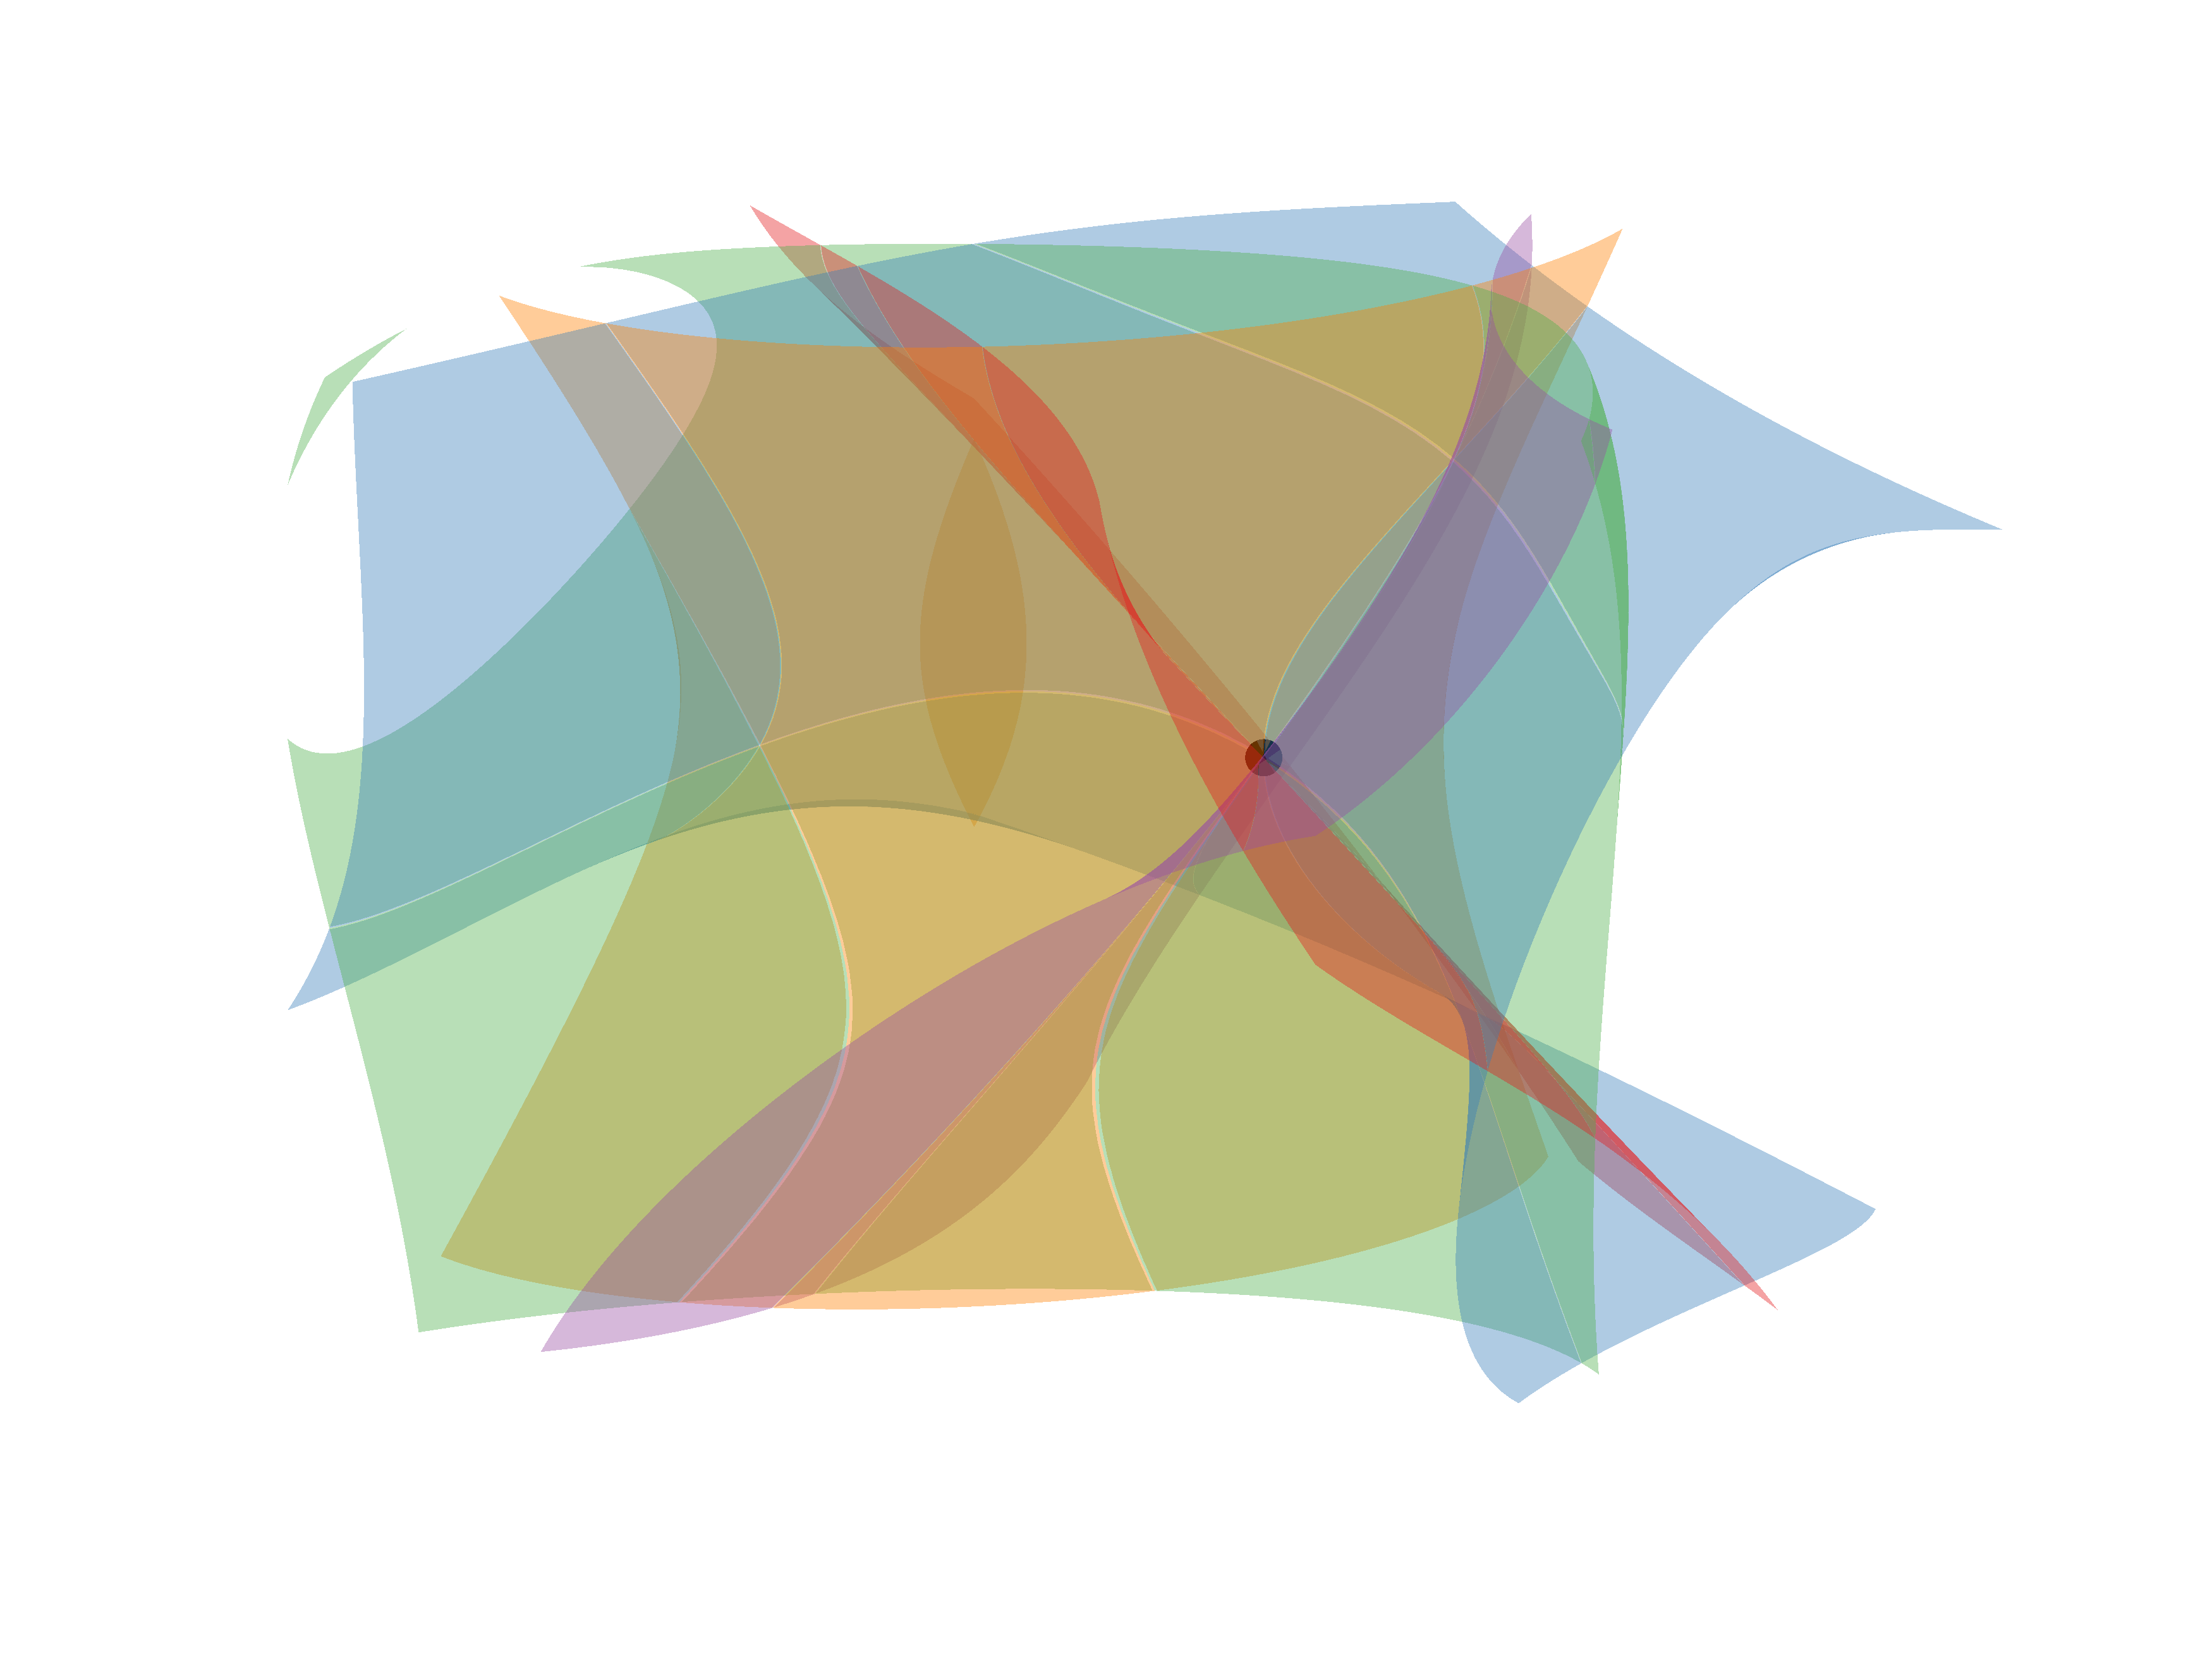
\includegraphics[width=\textwidth]{"images/e5c3_example1.png"}
		\subcaption{Die fünf kubischen Hyperflächen aus System \eqref{eqn:example5C3_1}.}
	\end{subfigure}
\end{figure}
\begin{figure}[H]\ContinuedFloat
	\begin{subfigure}[b]{0.8\textwidth}
		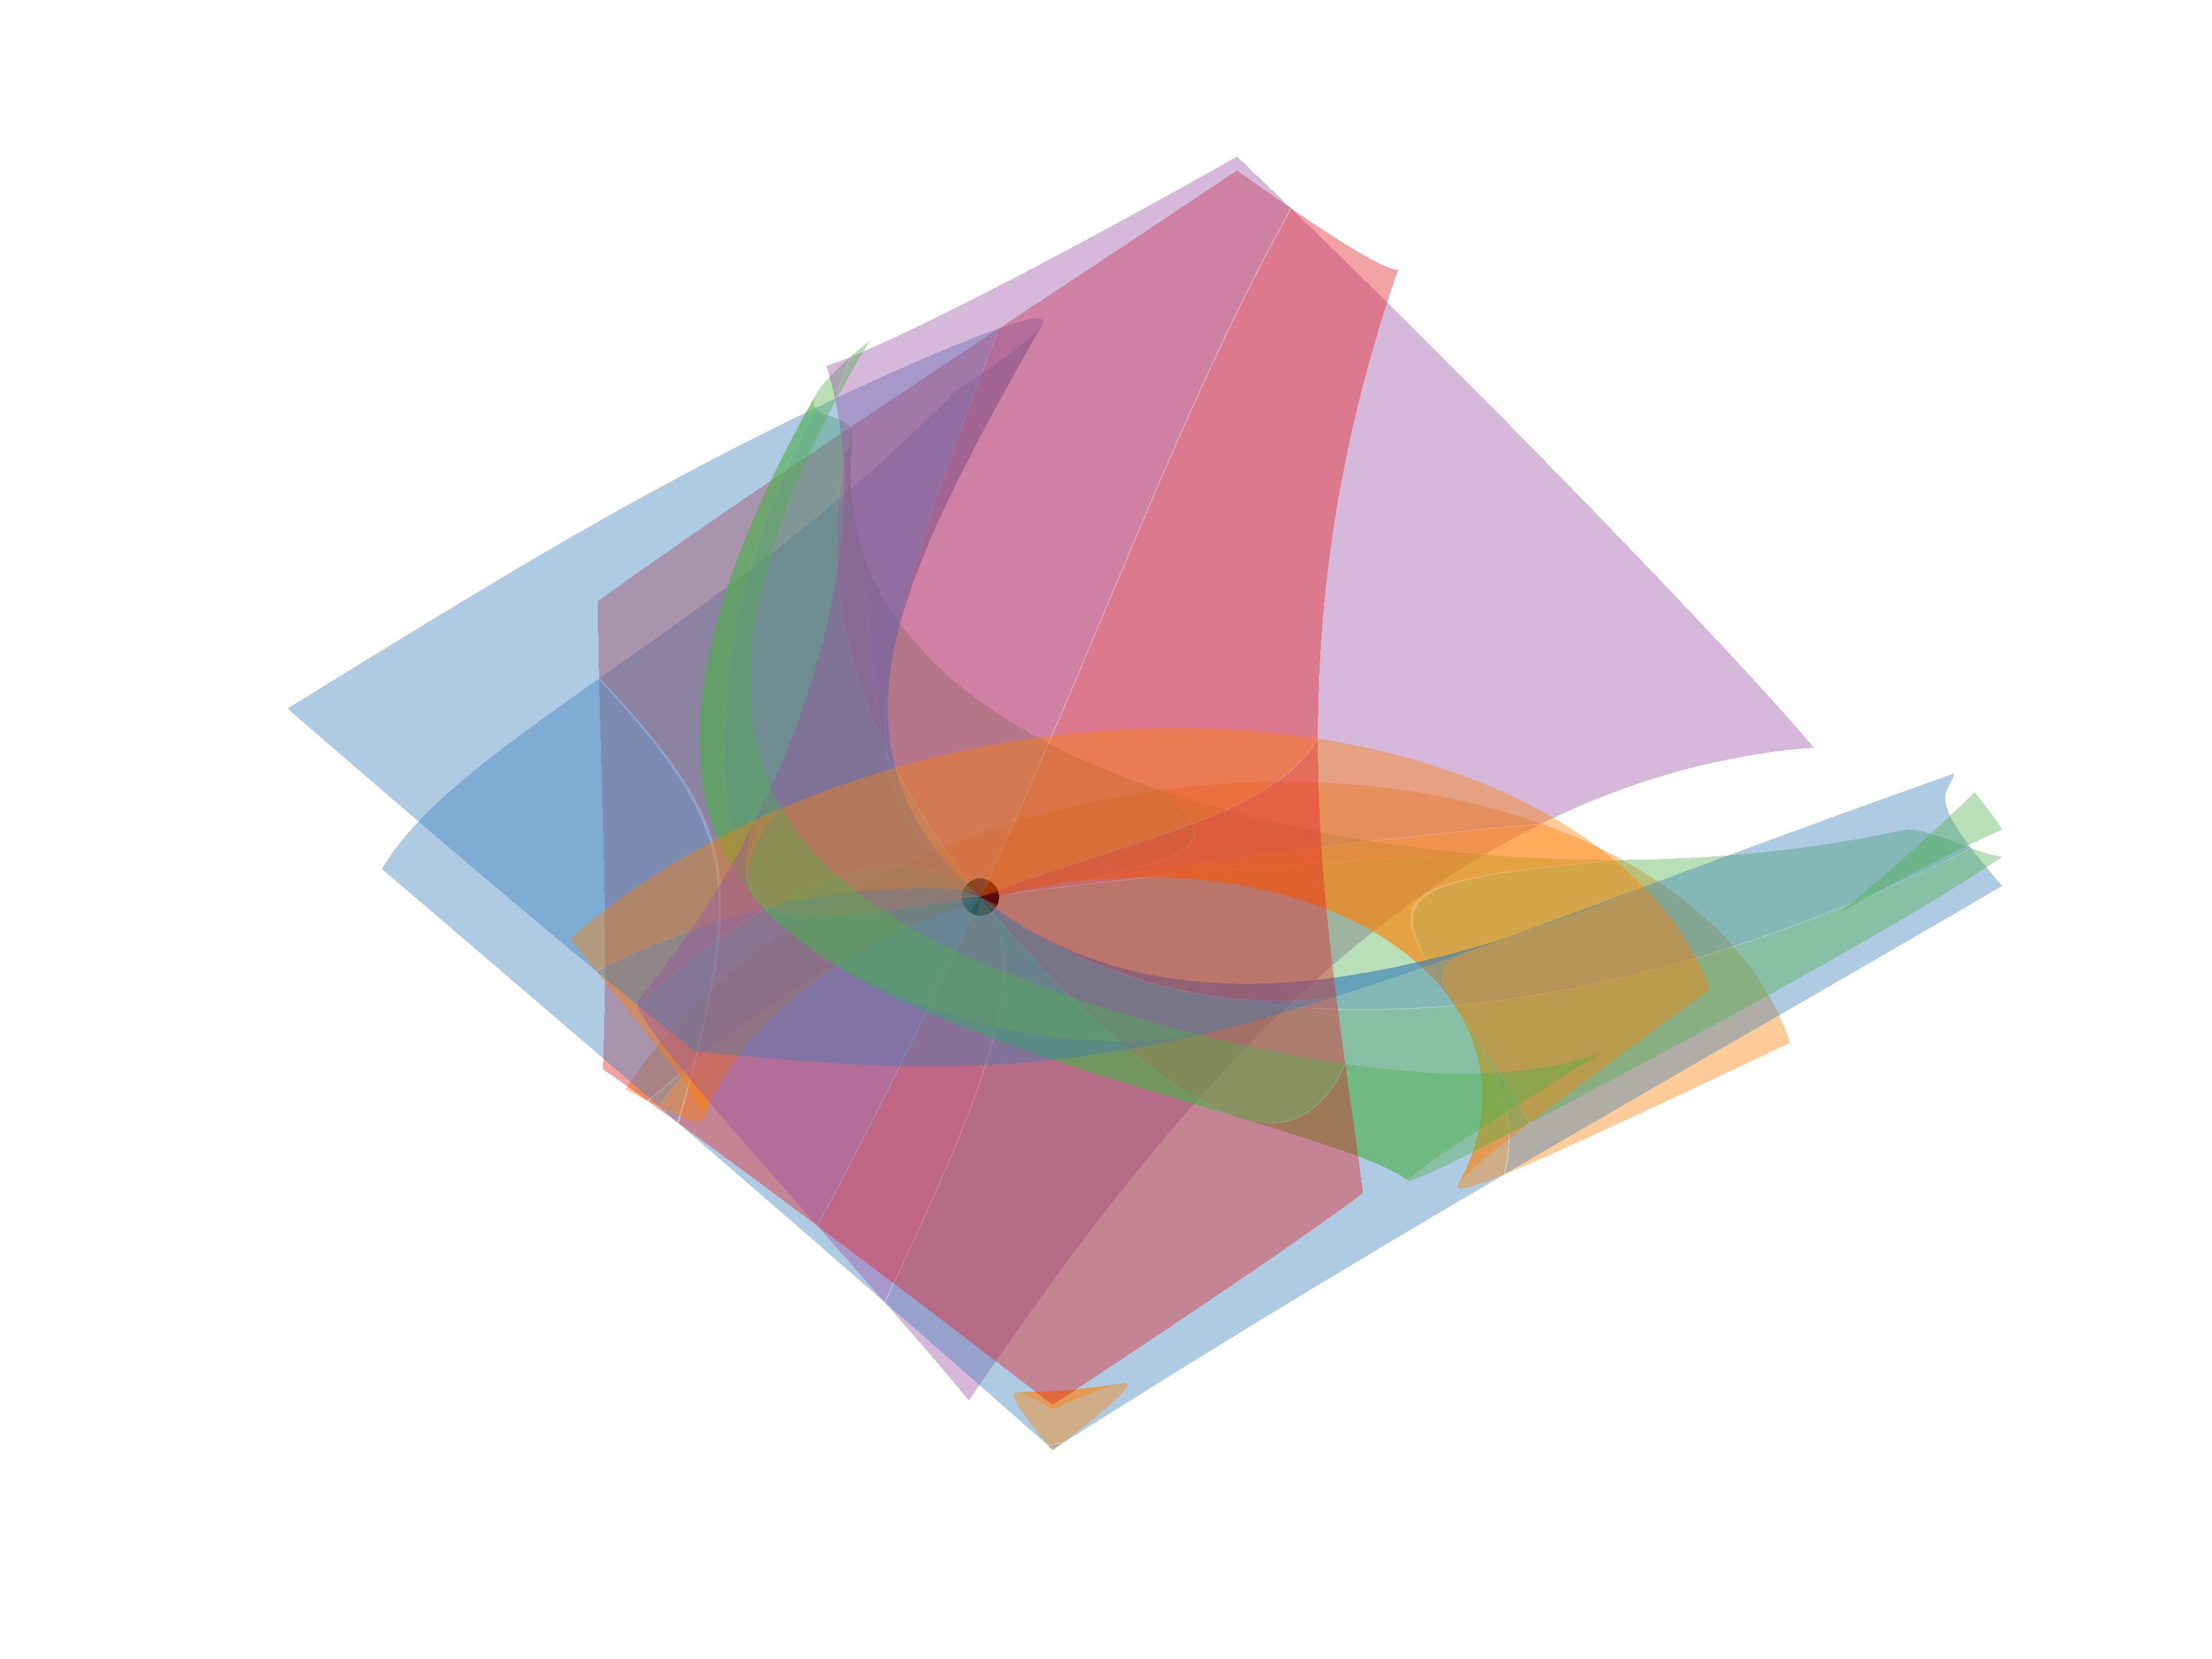
\includegraphics[width=\textwidth]{"images/e5c3_example1_angle.png"}
		\subcaption{Geometrie der fünf kubischen Hyperflächen aus einem anderen Winkel.}
	\end{subfigure}
	\caption{Geometrie der fünf kubischen Hyperflächen aus Beispiel  \eqref{eqn:example5C3_1}.}
\end{figure}
\begin{example}
	\label{ex:5C3_2}
	Für das Gleichungssystem
	\begin{equation*}\label{eqn:example5C3_2}
		\small
		\begin{alignedat}{1}
			3\,x^3+4\,x^2\,y+4\,x^2\,z+5\,x^2+6\,x\,y^2+5\,x\,z^2
			+2\,x\,z+3\,x+2\,y^3&\ldots\\
			+6\,y^2\,z+3\,y^2+5\,y\,z^2+6\,y\,z+3\,y+4&=0,\\ 5\,x^3+6\,x^2\,y+x^2\,z+2\,x^2+4\,x\,y^2+6\,x\,y+4\,x\,z^2
			+4\,x\,z+6\,x&\ldots\\
			+5\,y^3+6\,y^2\,z+6\,y^2+2\,y\,z^2+5\,y+z^3+1&=0,\\ 2\,x^3+5\,x^2\,y+5\,x^2\,z+x^2+x\,y^2+5\,x\,y+x\,z^2+3\,x\,z
			+3\,y^3+2\,y^2\,z&\ldots\\
			+3\,y^2+5\,y\,z^2+2\,y\,z+3\,y+z^3+4\,z^2+3\,z+2&=0,\\ 2\,x^3+5\,x^2\,y+5\,x^2\,z+5\,x^2+4\,x\,y^2+x\,z+6\,x
			+4\,y^3+2\,y^2&\ldots\\
			+y\,z^2+y\,z+6\,z^3+2\,z^2+5\,z+2&=0,\\ 3\,x^3+2\,x^2\,y+4\,x^2\,z+5\,x\,y^2+2\,x\,y+4\,x\,z^2
			+4\,x\,z+2\,x+4\,y^3&\ldots\\
			+2\,y^2+4\,y\,z^2+y\,z+z^3+2\,z^2+1&=0
		\end{alignedat}
	\end{equation*}
	über $\F{7}$ liefert der Algorithmus die Lösungen 
	\begin{equation*}
		\begin{alignedat}{5}
			&\left( x_{1},y_{1},z_{1}\right) &=& \left(6,2,5 \right).&&
		\end{alignedat}
	\end{equation*}
\end{example}
\newpage
\section{Lösen des 4C3-Problems}
\subsection{Formulierung eines 4C3-Algorithmus}\label{sec:4C3_alg}
Gegeben sei ein $4C3$-Problem über einem Körper $K$ mit zugehöriger Koeffizientenmatrix $C \in K^{4 \times 20}$.

Analog zu dem Vorgehen in Abschnitt \ref{sec:E3Q3} betrachten wir $4$ Gleichungen in $K\left[ X_{1}\right] \left[X_{2},X_{3}\right] $ anstatt $K\left[ X_{1},X_{2},X_{3}\right]$. Zunächst verstauen wir $X_{1}$ in dem Koeffizientenring und teilen die verbleibenden Monome in den Unbestimmten $X_{2},\ X_{3}$ in zwei Gruppen $\{X_{2}^3,X_{3}^3,X_{2}^2X_{3},X_{2}X_{3}^2\}$ und $\{X_{2}^2,X_{2}X_{3},X_{3}^2,X_{2},X_{3},1\}$ auf.

Teilen wir jetzt die Koeffizientenmatrix $C$ auf beide Gruppen auf ergibt sich 

\begin{equation*}
	-A
	\begin{pmatrix}[1.5]
		X_{2}^3\\
		X_{2}^2X_{3}\\
		X_{2}X_{3}^2\\
		X_{3}^3
	\end{pmatrix}
	=
	\begin{pmatrix}[1.75]
		\vert & \vert & \vert & \vert & \vert& \vert \\
		p_{i,1}&p_{i,2}& p_{i,3}& p_{i,4}& p_{i,5}& p_{i,6}\\
		\vert & \vert & \vert & \vert & \vert& \vert
	\end{pmatrix}
	\begin{pmatrix}
		X_{2}^2\\
		X_{2}X_{3}\\
		X_{3}^2\\
		X_{2}\\
		X_{3}\\
		1
	\end{pmatrix}
\end{equation*}
wobei $A \in K^{4 \times 4}$ die Koeffizientenmatrix
\begin{equation}
	A = 
	\begin{pmatrix}[1.1]
		c_{1,7}& c_{1,8}& c_{1,9}& c_{1,10}\\
		c_{2,7}& c_{2,8}& c_{2,9}& c_{2,10}\\
		c_{3,7}& c_{3,8}& c_{3,9}& c_{3,10}\\
		c_{4,7}& c_{4,8}& c_{4,9}& c_{4,10}
	\end{pmatrix}
\end{equation}
ist und $p_{i,1}, \ldots, p_{i,6}$ Polynome
\begin{equation}
	\begin{alignedat}{4}
		p_{i1}= \ &&&c_{i,4}\,X_{1}+&c_{i,14},\\
		p_{i2}= \ &&&c_{i,5}\,X_{1}+&c_{i,15},\\
		p_{i3}= \ &&&c_{i,6}\,X_{1}+&c_{i,16},\\
		p_{i4}= \ &&c_{i,2}\,X_{1}^2+&c_{i,12}\,X_{1}+&c_{i,18},\\
		p_{i5}= \ &&c_{i,3}\,X_{1}^2+&c_{i,13}\,X_{1}+&c_{i,19},\\
		p_{i6}= \ &c_{i,1}\,X_{1}^3+&c_{i,11}\,X_{1}^2+&c_{i,17}\,X_{1}+&c_{i,20},
	\end{alignedat}
\end{equation}
für $i\in \{1,2,3,4\}$ sind.
Wir setzen hier die Invertierbarkeit von $A$ voraus und multiplizieren jetzt die Gleichung von links mit der zu $A$ inversen Matrix $A^{-1}$ durch und erhalten
\begin{equation*}
	\begin{pmatrix}[1.5]
		X_{2}^3\\
		X_{2}^2X_{3}\\
		X_{2}X_{3}^2\\
		X_{3}^3\\
	\end{pmatrix}
	=
	\begin{pmatrix}[1.5]
		p'_{11}(X_{1})&p'_{12}(X_{1})& p'_{13}(X_{1})& p'_{14}(X_{1})& p'_{15}(X_{1})& p'_{16}(X_{1})\\
		p'_{21}(X_{1})&p'_{22}(X_{1})& p'_{23}(X_{1})& p'_{24}(X_{1})& p'_{25}(X_{1})& p'_{26}(X_{1})\\
		p'_{31}(X_{1})&p'_{32}(X_{1})& p'_{33}(X_{1})& p'_{34}(X_{1})& p'_{35}(X_{1})& p'_{36}(X_{1})\\
		p'_{41}(X_{1})&p'_{42}(X_{1})& p'_{43}(X_{1})& p'_{44}(X_{1})& p'_{45}(X_{1})& p'_{46}(X_{1})
	\end{pmatrix}
	\begin{pmatrix}
		X_{2}^2\\
		X_{2}X_{3}\\
		X_{3}^2\\
		X_{2}\\
		X_{3}\\
		1
	\end{pmatrix}.
\end{equation*}
Damit die Substitution wie in Abschnitt \ref{sec:4C3} funktionieren kann, müssen alle Polynome
$p'_{i,j}(X_{1})$ für $i \in \{1,2,3,4\}, \ j \in \{1,2,3\}$ das Nullpolynom sein. 

Diese Bedingungen führen also auf das Gleichungssystem
\begin{equation}
	A^{-1} \cdot \begin{pmatrix}[1.75]
		\vert & \vert & \vert \\
		p_{i,1}&p_{i,2}& p_{i,3}\\
		\vert & \vert & \vert
	\end{pmatrix}
	= 0_{K^{4 \times 3}}.
\end{equation}
Für die Matrix $A^{-1}$ gilt aber \begin{equation*}
	\det{\left(A^{-1}\right)} \neq 0,
\end{equation*} womit nach Satz \ref{prop:LGS} die einzige Lösung für das Gleichungssystem die triviale Lösung ist.
Somit müssen wir also
\begin{equation*}
	c_{i,j} = 0 , \ \text{für alle} \ i \in \{1,2,3,4\} \ \text{und alle} \ j \in \{4,5,6,14,15,16\},
\end{equation*}
voraussetzen, um den Algorithmus durchführen zu können.
Nur dann kommen beim Substituieren in die Identitäten
\begin{equation*}
	\begin{alignedat}{3}
		X_{3}^3&	\left( X_{2}^3\right)  &=& \left( X_{2}^2X_{3}\right) 	\left( X_{2}X_{3}^2\right), \\
		X_{3}&\left( X_{2}^3\right) &=&\left( X_{2}^2X_{3}\right) X_{2},\\
		X_{3}^2&	\left( X_{2}^3\right)  &=& \left(  X_{2}X_{3}^2\right) 	X_{2}^2,\\
		X_{2}&	\left( X_{3}^3\right)  &=& \left( X_{2}X_{3}^2\right) 	X_{3},\\
		X_{2}^3&	\left( X_{2}X_{3}^2\right)  &=& \left( X_{2}^2X_{3}\right)\left( X_{2}^2X_{3}\right),\\
		X_{3}^3&	\left( X_{2}^2X_{3}\right)  &=& \left( X_{2}X_{3}^2\right)\left( X_{2}X_{3}^2\right),\\
	\end{alignedat}
\end{equation*}
keine Monome vierten Grades aus $K[X_1][X_2,X_3]$ vor.
Nach zweimaliger Substitution kommen in den $6$ Gleichungen auch keine Monome dritten Grades mehr vor und wir können das Gleichungssystem
\begin{equation}
	M(X_{1})\begin{pmatrix}[1.3]
		X_{2}^2,
		X_{2}X_{3},
		X_{3}^2,
		X_{2},
		X_{3},
		1
	\end{pmatrix}^\top=0
\end{equation}
bilden, wobei $M(X_{1}) \in K[X_{1}]^{6 \times 6}$ die Matrix
\begin{equation}
	\small
	M = \begin{pmatrix}[1.3]
		m_{11}^{\left[ 4\right]}\left( X_{1}\right) & m_{12}^{\left[ 4\right]}\left( X_{1}\right) & m_{13}^{\left[ 4\right]}\left( X_{1}\right) & m_{14}^{\left[ 5\right]}\left( X_{1}\right) & m_{15}^{\left[ 5\right]}\left( X_{1}\right) & m_{16}^{\left[ 6\right]}\left( X_{1}\right)\\
		m_{21}^{\left[ 3\right]}\left( X_{1}\right) & 0 & m_{23}^{\left[ 3\right]}\left( X_{1}\right)& m_{24}^{\left[ 4\right]}\left( X_{1}\right) & m_{25}^{\left[ 4\right]}\left( X_{1}\right)& m_{26}^{\left[ 5\right]}\left( X_{1}\right) \\
		m_{31}^{\left[ 3\right]}\left( X_{1}\right) & 0 & m_{33}^{\left[ 3\right]}\left( X_{1}\right)& m_{34}^{\left[ 4\right]}\left( X_{1}\right) & m_{35}^{\left[ 4\right]}\left( X_{1}\right)& m_{36}^{\left[ 5\right]}\left( X_{1}\right) \\
		m_{41}^{\left[ 2\right]}\left( X_{1}\right) & m_{42}^{\left[ 2\right]}\left( X_{1}\right) & m_{43}^{\left[ 2\right]}\left( X_{1}\right)& m_{44}^{\left[ 3\right]}\left( X_{1}\right) & m_{45}^{\left[ 3\right]}\left( X_{1}\right)& 0 \\
		m_{51}^{\left[ 4\right]}\left( X_{1}\right) & m_{52}^{\left[ 4\right]}\left( X_{1}\right) & m_{53}^{\left[ 4\right]}\left( X_{1}\right) & m_{54}^{\left[ 5\right]}\left( X_{1}\right) & m_{55}^{\left[ 5\right]}\left( X_{1}\right) & m_{56}^{\left[ 6\right]}\left( X_{1}\right)\\
		m_{61}^{\left[ 4\right]}\left( X_{1}\right) & m_{62}^{\left[ 4\right]}\left( X_{1}\right) & m_{63}^{\left[ 4\right]}\left( X_{1}\right) & m_{64}^{\left[ 5\right]}\left( X_{1}\right) & m_{65}^{\left[ 5\right]}\left( X_{1}\right) & m_{66}^{\left[ 6\right]}\left( X_{1}\right)\\
	\end{pmatrix}
\end{equation}
ist.\\
Dabei ist $\det{M(X_{1})}$ ein Polynom 24. Grades und dessen Nullstellen $\tilde{x}_{1_{i}}$ sind genau die Lösungskandidaten des Usrprungssystems.
Wir setzen jeden dieser bis zu 24 Lösungskandidaten $\tilde{x}_{1_{i}}$ in die Matrix $M(X_{1})$ ein und erhalten 
\begin{equation}\label{eqn:low_rank_system_4C3}
	\tilde{M}\begin{pmatrix}[1.3]
		X_{2}^2,
		X_{2}X_{3},
		X_{3}^2,
		X_{2},
		X_{3},
		1
	\end{pmatrix}^{\top} = 	M(\tilde{x}_{1_{i}})\begin{pmatrix}[1.3]
		X_{2}^2,
		X_{2}X_{3},
		X_{3}^2,
		X_{2},
		X_{3},
		1
	\end{pmatrix}^{\top}=0,
\end{equation}
wobei aufgrund der Berechnung von $\tilde{x}_{1_{i}}$ 
\begin{equation*}
	r \coloneqq \text{rank}(\tilde{M}) < 6
\end{equation*} gilt.\\
Um das Gleichungssystem \eqref{eqn:low_rank_system_4C3} zu lösen, nehmen wir die Variablen zunächst als unabhängig an und dann lösen wir das lineare Gleichungssystem
\begin{equation}\label{eqn:low_rank_system_ind_4C3}
	\tilde{M} \cdot \begin{pmatrix}
		s,
		t,
		u,
		v,
		w,
		1
	\end{pmatrix}^{\top}
	=0.
\end{equation}
Der Lösungsraum dieses Gleichungssystems ist ein $(5-r)$-dimensionaler affiner Unterraum welcher die Gestalt ${v_0 + U \subset K^6}$ besitzt. Eine Basis von $U$ kann mithilfe des Gauß Algorithmus bestimmt werden. Die gesuchte Lösung zu \eqref{eqn:low_rank_system_4C3} muss aber zusätzlich auf der Fläche \begin{equation*}
	{S \coloneqq \{(v^2,v\cdot w,w^2,v,w,1) : v,w \in K\}}
\end{equation*} liegen. Der Schnitt $v_0 + U \cap S $ beinhaltet somit alle Lösungen $(\tilde{x}_{2},\tilde{x}_{3})$ zu gegebenen Lösungskandidaten $\tilde{x}_{1_{i}}$.\\
Das genaue Vorgehen zum Lösen des resultierenden Gleichungssystems hängt jetzt sowohl vom Rang der Matrix als auch deren spezifischen normierten Zeilenstufenform ab. So ergeben sich $30$ verschiedene konsistente Fälle, welche analog zu dem Vorgehen in Abschnitt \ref{sec:5C3_GLS} gelöst werden können.

\begin{remark}
	Die Anforderungen an die Koeffizienten des Gleichungssystems schränken die Systeme, welche wir mit dem Algorithmus lösen können auf solche der Form
	\begin{equation}
		\small
		\begin{alignedat}{1}
			\mu_{i,1}X_{j}^3+\mu_{i,2}X_{k}^3+\mu_{i,3}X_{j}^2X_{k}+\mu_{i,4}X_{j}^2X_{l}+\mu_{i,5}X_{k}^2X_{l}+\mu_{i,6}X_{k}X_{l}^2+\mu_{i,7}X_{l}^3&...\\
			+\mu_{i,8}X_{j}^2+\mu_{i,9}X_{j}X_{k}+\mu_{i,10}X_{j}X_{l}+\mu_{i,11}X_{j}+\mu_{i,12}X_{k}+\mu_{i,13}X_{l}+\mu_{i,14} &= 0,
		\end{alignedat}
	\end{equation}
	für $i \in \{1,2,3,4\}$.
\end{remark}

\newpage
%\subsection{Vollständige Diskussion der Gleichungssysteme}\label{sec:4C3_GLS}
%Im Folgenden betrachten wir alle verschiedenen normierten Zeilenstufenformen, welche die Matrix $\tilde{M}$ in Gleichung \eqref{eqn:low_rank_system_ind_4C3} annehmen kann.
%Um die verschiedenen normierten Zeilenstufenformen zu unterscheiden verwenden wir dabei die Notation $R_{i_1,\ldots,i_j}$, wobei $\{i_1,\ldots,i_j\}$ die Spaltenindizes sind, in denen die $j$ Einheitsvektoren zu finden sind.
%\subsubsection*{Fall $\text{R}_{1}$}
%Der Gauß Algorithmus liefert die normierte Zeilenstufenform des Systems \eqref{eqn:low_rank_system_ind_4C3} als
%\begin{equation*}\label{eqn:rref_r1_4C3}
%	\begin{alignedat}{-1}
%		\text{rref}(\tilde{M}) &=& 
%		\left( \begin{array}{cccccc}
%			1&r_{11}&r_{12}&r_{13}&r_{14}&r_{15}\\
%			0&0&0&0&0&0\\
%			0&0&0&0&0&0\\
%			0&0&0&0&0&0\\
%			0&0&0&0&0&0\\
%			0&0&0&0&0&0
%		\end{array}
%		\right)
%	\end{alignedat}
%\end{equation*}
%
%und somit einen Lösungsraum der Gestalt
%\begin{equation*}
%	\begin{pmatrix}
%		-r_{11}\\
%		1\\
%		0\\
%		0\\
%		0\\
%		0
%	\end{pmatrix}t +
%	\begin{pmatrix}
%		-r_{12}\\
%		0\\
%		1\\
%		0\\
%		0\\
%		0
%	\end{pmatrix}u +
%	\begin{pmatrix}
%		-r_{13}\\
%		0\\
%		0\\
%		1\\
%		0\\
%		0
%	\end{pmatrix}v +
%	\begin{pmatrix}
%		-r_{14}\\
%		0\\
%		0\\
%		0\\
%		1\\
%		0
%	\end{pmatrix}w +
%	\begin{pmatrix}
%		-r_{15}\\
%		0\\
%		0\\
%		0\\
%		0\\
%		1
%	\end{pmatrix}.
%\end{equation*}
%\subsubsection*{Fall $\text{R}_{1,2,3,4,5}$}
%Der Gauß Algorithmus liefert die normierte Zeilenstufenform des Systems \eqref{eqn:low_rank_system_ind_4C3} als
%\begin{equation*}\label{eqn:rref_r12345_4C3}
%	\begin{alignedat}{-1}
%		\text{rref}(\tilde{M}) &=& 
%		\left( \begin{array}{cccccc}
%			1&0&0&0&0&r_{11}\\
%			0&1&0&0&0&r_{21}\\
%			0&0&1&0&0&r_{31}\\
%			0&0&0&1&0&r_{41}\\
%			0&0&0&0&1&r_{51}\\
%			0&0&0&0&0&0
%		\end{array}
%		\right)
%	\end{alignedat}
%\end{equation*}
%
%und somit einen Lösungsraum der Gestalt
%\begin{equation*}
%	\begin{pmatrix}
%		-r_{11}\\
%		-r_{21}\\
%		-r_{31}\\
%		-r_{41}\\
%		-r_{51}\\
%		1
%	\end{pmatrix}.
%\end{equation*}
%\newpage
\subsection{Anwendung des 4C3-Algorithmus auf Beispiele}
Da das 4C3-Problem, analog zum 5C3-Problem, ein überbestimmtes Gleichungssystem liefert existiert im Allgemeinen keine Lösung. In diesem Kapitel betrachten wir die Ergebnisse des 4C3-Algorithmus anhand einiger spezieller Systeme, welche eine Lösung besitzen.
\begin{example}\label{ex:4C3_1}
	Betrachten wir das Gleichungssystem
	\begin{equation}\label{eqn:example4C3_1}
		\begin{alignedat}{-1}
2\,x+2\,y+3\,z-x\,y+5\,x\,z-4\,x^2\,z+5\,x^3-y^3-3&=0,\\ x-4\,y-4\,z+4\,x\,y-4\,x\,z+2\,x^2\,y+x^2\,z-y^2\,z-3\,x^3+4&=0,\\ x^2\,y-4\,y-2\,z-2\,x\,y-4\,x\,z-3\,x-4\,x^2\,z-y\,z^2-x^3+2&=0,\\ 3\,x-3\,y-2\,z+x\,y-4\,x\,z+2\,x^2\,y+4\,x^2\,z+4\,x^3-z^3+3&=0
		\end{alignedat}
	\end{equation}
	über $\R$ so erhalten wir mit dem 4C3-Algorithmus die Lösung
	\begin{equation*}
		\begin{alignedat}{5}
			&\left( x_{1},y_{1},z_{1}\right) &=& \left(0, 0, 1 \right).&&
		\end{alignedat}
	\end{equation*}
\end{example}
	\begin{figure}[H]
\begin{subfigure}[b]{0.8\textwidth}
			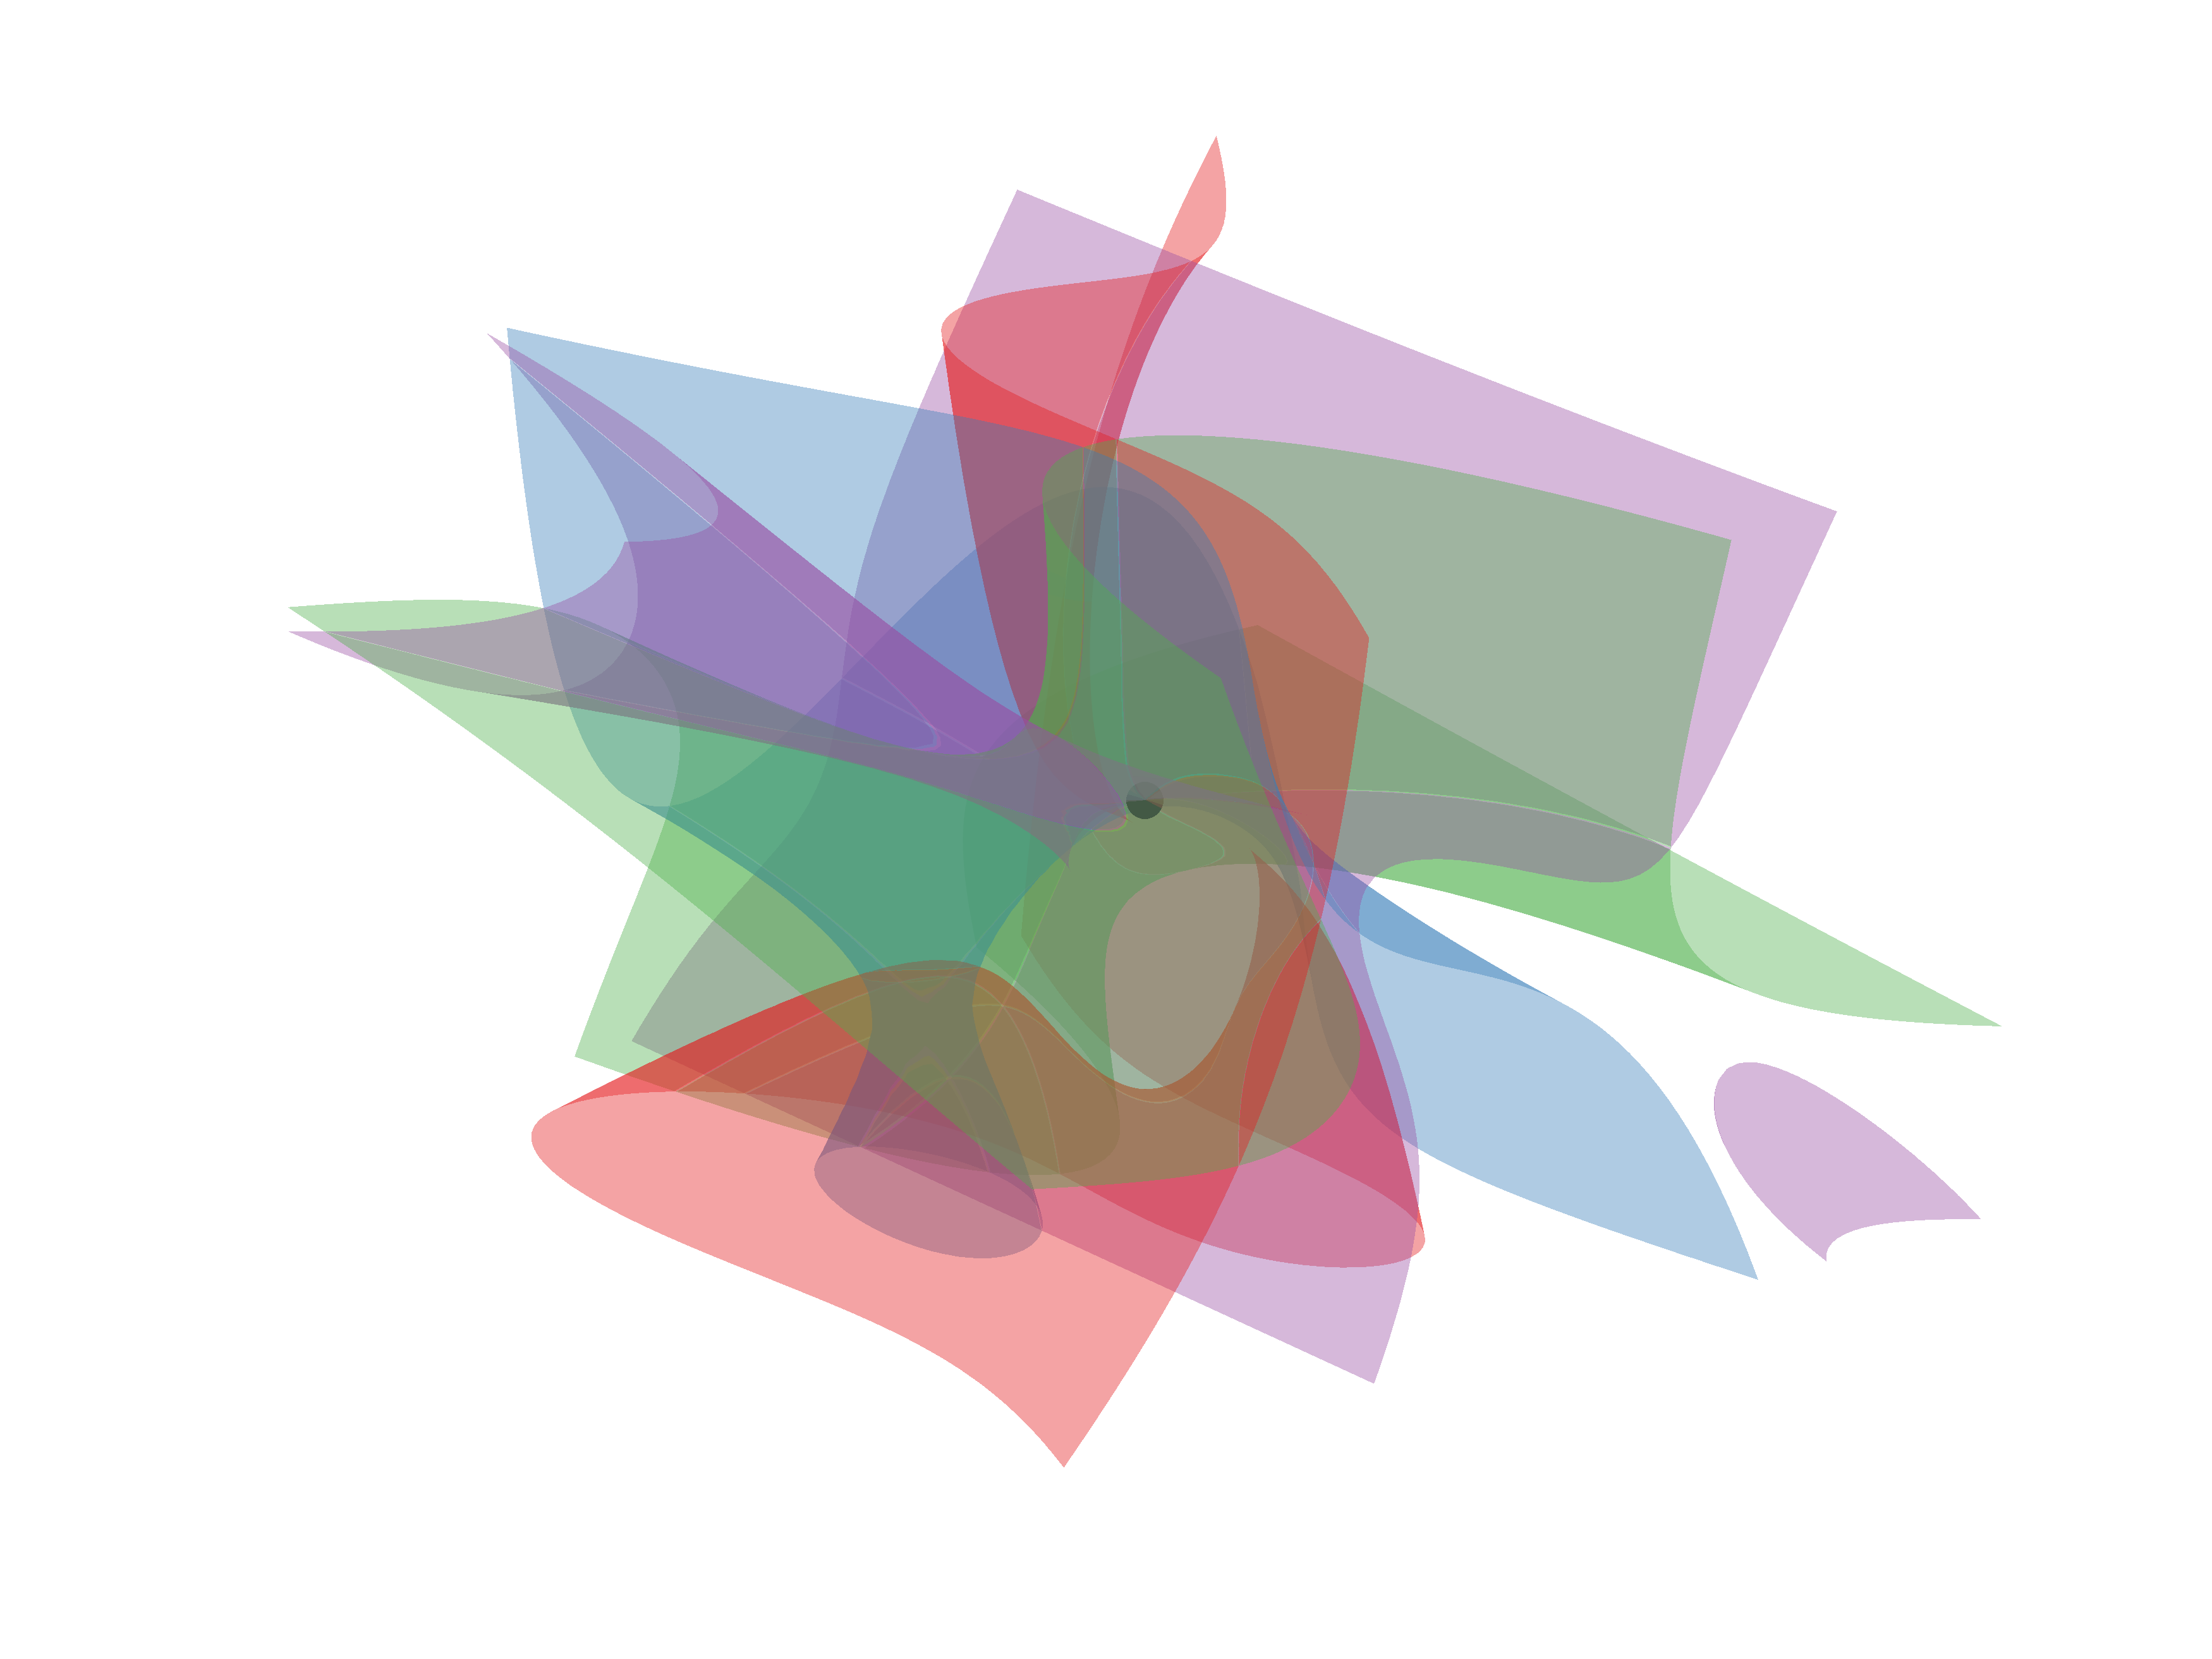
\includegraphics[width=\textwidth]{"images/e4c3_example1.png"}
		\subcaption{Die vier kubischen Flächen (rot,blau,grün und lila) aus Beispiel \ref{ex:4C3_1} und deren gemeinsamer Schnittpunkt.}
\end{subfigure}
	\end{figure}
	\begin{figure}[H]\ContinuedFloat
		\begin{subfigure}[b]{0.8\textwidth}
			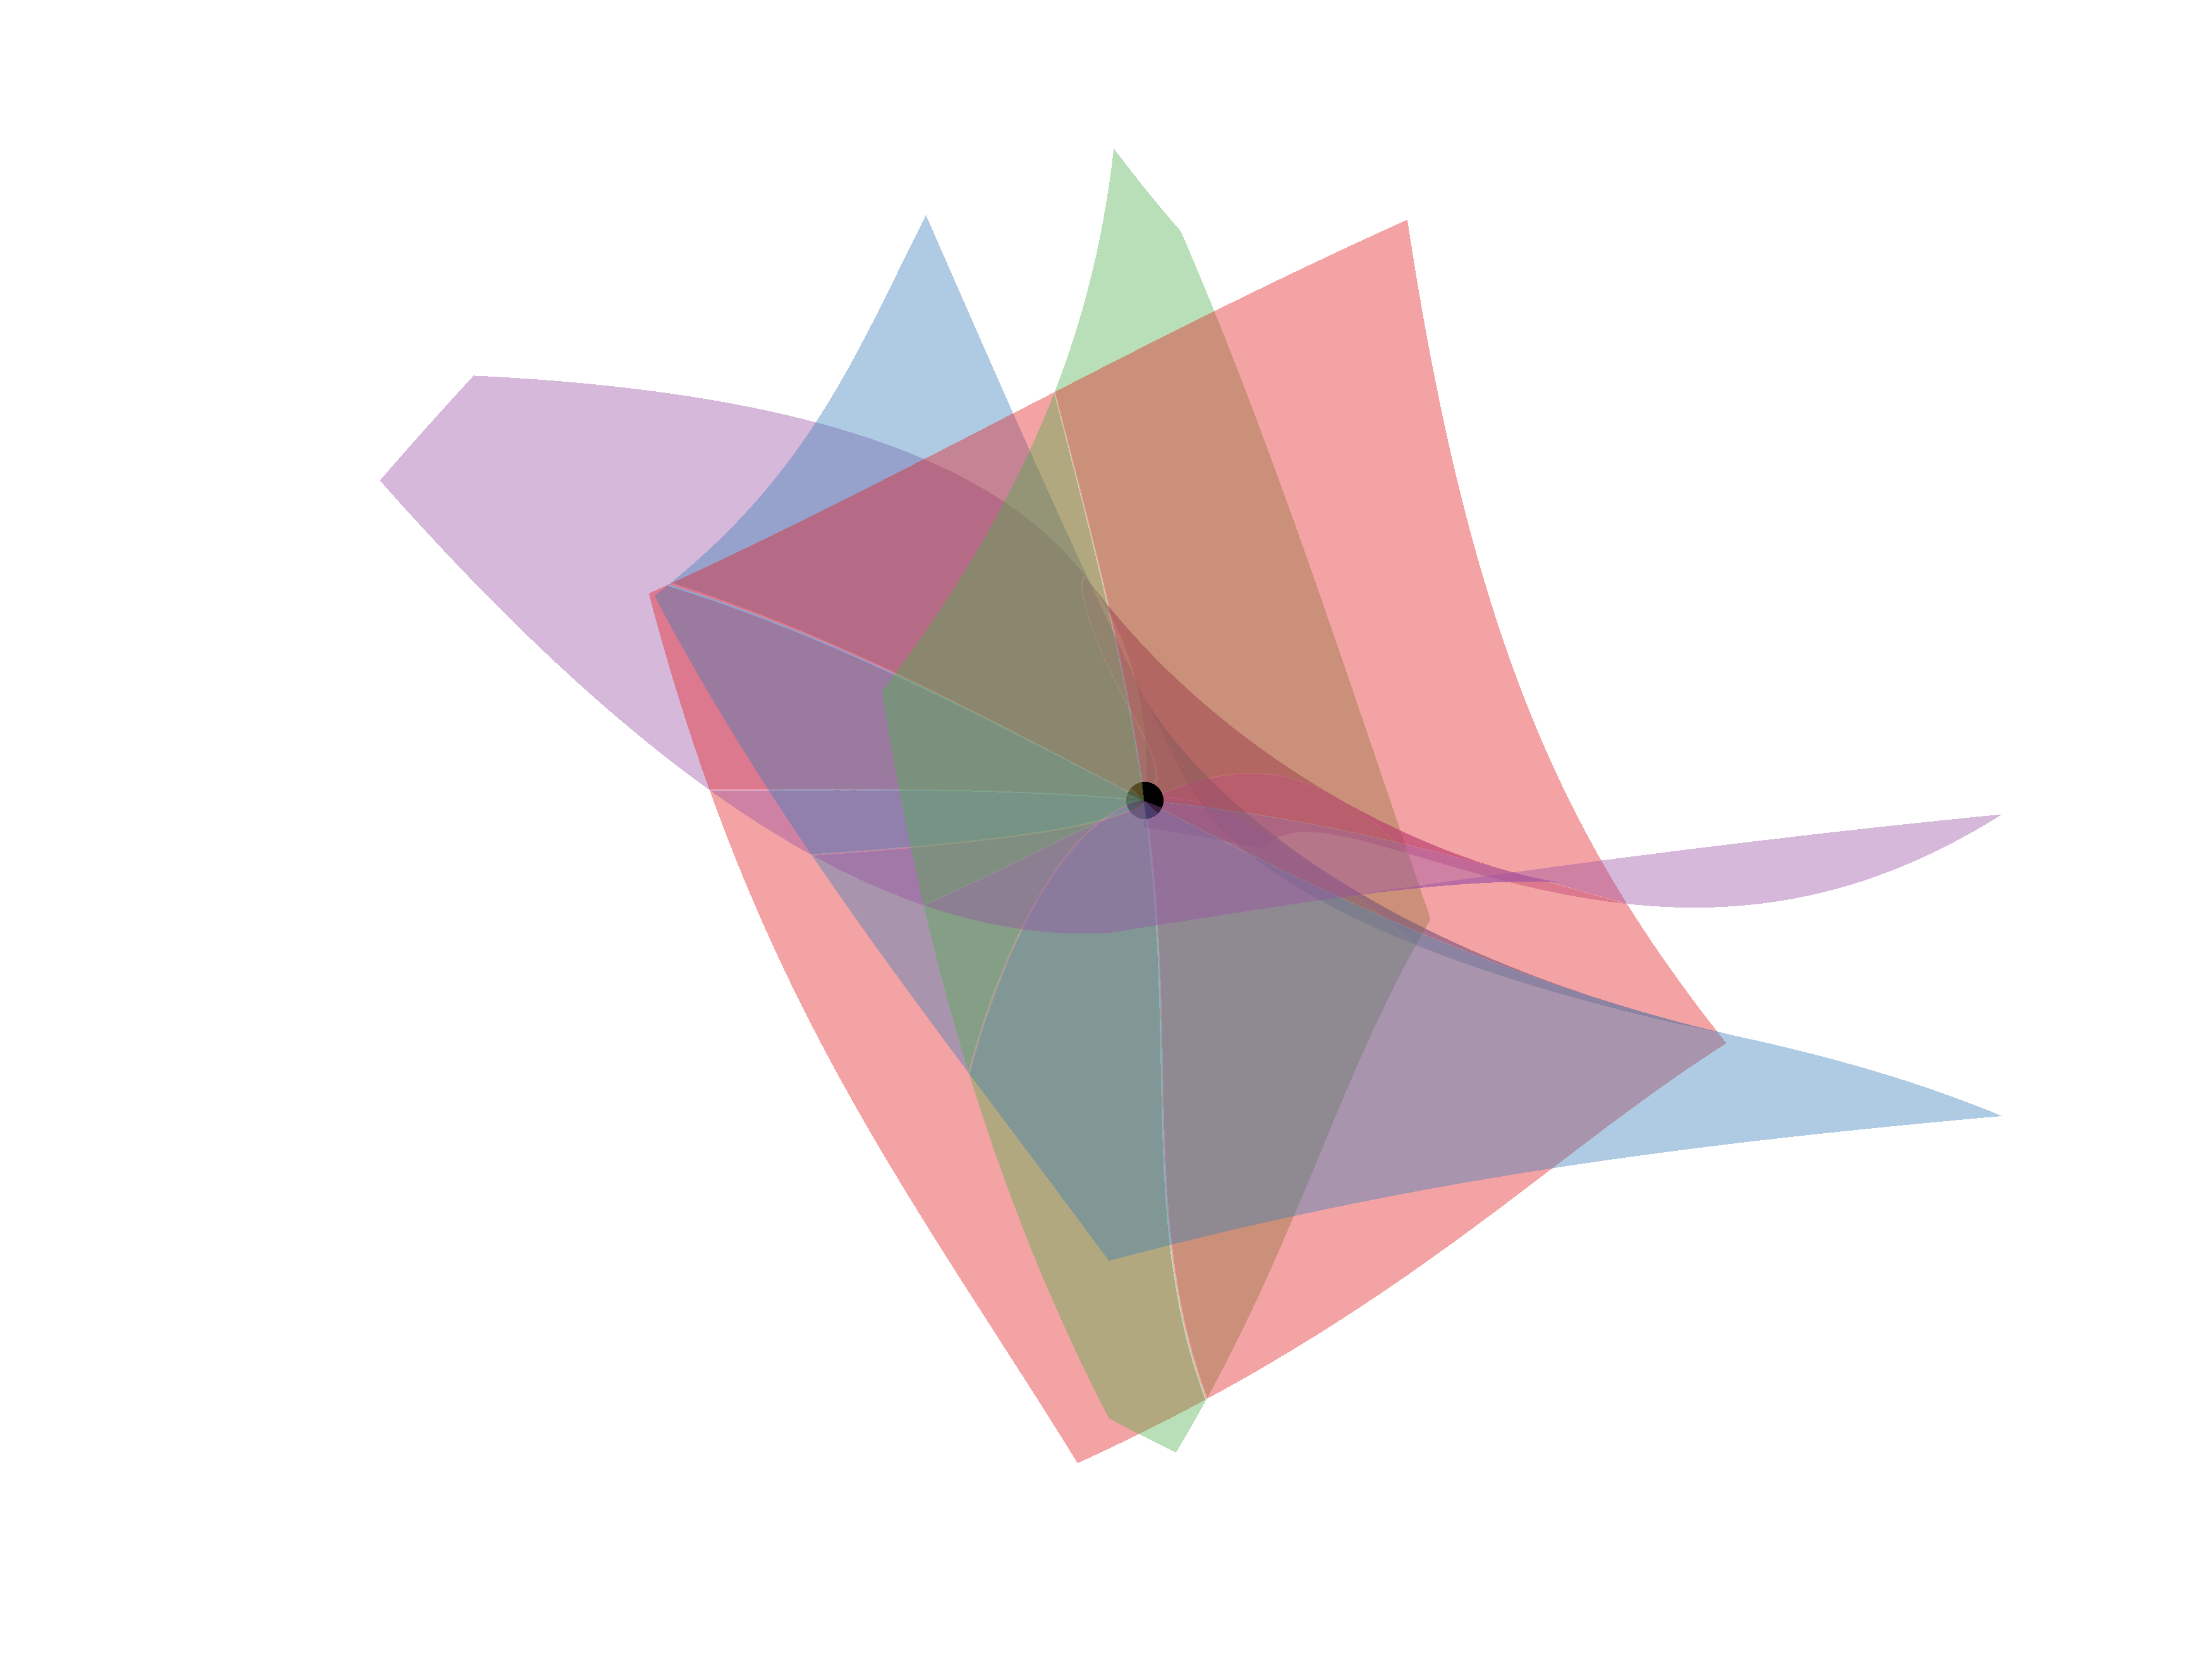
\includegraphics[width=\textwidth]{"images/e4c3_example1_zoom.png"}
			\subcaption{Die vier kubischen Flächen und deren gemeinsamer Schnittpunkt in näherer Umgebung.}
		\end{subfigure}
		\caption{Die Geometrie der vier kubischen Hyperflächen des \newline Systems aus Beispiel \ref{ex:4C3_1}.}
	\end{figure}
	\begin{example}
		Betrachten wir das Gleichungssystem
		\begin{equation}
			\begin{alignedat}{1}
				10\,x^3+6\,x^2\,y+2\,x\,y^2+13\,x\,z^2+8\,x\,z+17\,x+17\,y^3+15\,y\,z^2&\ldots\\+3\,y\,z+15\,y+11\,z^3+10\,z^2+6\,z+6&=0,\\ 15\,x^3+8\,x^2\,y+5\,x\,y^2+5\,x\,z^2+7\,x\,z+10\,x+12\,y^3+11\,y\,z^2&\ldots\\+6\,y\,z+8\,y+5\,z^3+3\,z^2+10\,z+12&=0,\\ 16\,x^3+14\,x^2\,y+9\,x\,y^2+5\,x\,z^2+15\,x\,z+4\,y^3+18\,y\,z^2&\ldots\\+2\,y\,z+7\,y+15\,z^3+2\,z^2+13\,z+18&=0,\\ 14\,x^3+2\,x^2\,y+18\,x\,y^2+16\,x\,z^2+12\,x\,z+x+y^3+y\,z^2&\ldots\\+12\,y\,z+15\,y+3\,z^3+9\,z^2+16\,z+1&=0
			\end{alignedat}
		\end{equation}
		über $\F{19}$ so erhalten wir mit dem 4C3-Algorithmus die Lösung
		\begin{equation*}
			\begin{alignedat}{5}
				&\left( x_{1},y_{1},z_{1}\right) &=& \left(18, 6, 1 \right).&&
			\end{alignedat}
		\end{equation*}
	\end{example}

\newpage
\section{Lösen des 3C3-Problems}
\subsection{Formulierung eines 3C3-Algorithmus}\label{sec:3C3_alg}
Gegeben sei ein $3C3$-Problem über einem Körper $K$ mit zugehöriger Koeffizientenmatrix $C \in K^{4 \times 20}$.
Analog zu dem Vorgehen in Abschnitt \ref{sec:E3Q3} betrachten wir $3$ Gleichungen in $K\left[ X_{1}\right] \left[X_{2},X_{3}\right] $ anstatt $K\left[ X_{1},X_{2},X_{3}\right]$. Zunächst verstauen wir wieder $X_{1}$ in dem Koeffizientenring und teilen die verbleibenden Monome in den Unbestimmten $X_{2},\ X_{3}$ in zwei Gruppen $\{X_{2}^3,X_{2}^2X_{3},X_{2}X_{3}\}$ und $\{X_{2}X_{3}^2,X_{3}^3,X_{2}^2,X_{3}^2,X_{2},X_{3},1\}$ auf.
	
	
	Teilen wir jetzt die Koeffizientenmatrix $C$ auf beide Gruppen auf ergibt sich 
	
	\begin{equation*}
		-A
		\begin{pmatrix}[1.5]
			X_{2}^3\\
			X_{2}^2X_{3}\\
			X_{2}X_{3}
		\end{pmatrix}
		=
		\begin{pmatrix}[1.75]
			\vert & \vert & \vert & \vert & \vert& \vert& \vert \\
			p_{i,1}&p_{i,2}& p_{i,3}& p_{i,4}& p_{i,5}& p_{i,6}& p_{i,7}\\
			\vert & \vert & \vert & \vert & \vert& \vert& \vert
		\end{pmatrix}
		\begin{pmatrix}
			X_{2}X_{3}^2\\
			X_{3}^3\\
			X_{2}^2\\
			X_{3}^2\\
			X_{2}\\
			X_{3}\\
			1
		\end{pmatrix},
	\end{equation*}
	wobei $A \in K^{3 \times 3}$ die Koeffizientenmatrix
	\begin{equation}
		A = 
		\begin{pmatrix}[1.1]
			c_{1,7}& c_{1,8}&  c_{1,5}\,X_{1}+c_{1,15}\\
			c_{2,7}& c_{2,8}&  c_{2,5}\,X_{1}+c_{1,15}\\
			c_{3,7}& c_{3,8}&  c_{3,5}\,X_{1}+c_{1,15}
		\end{pmatrix}
	\end{equation}
	ist und $p_{i,1}, \ldots, p_{i,7}$ Polynome
	\begin{equation}
		\begin{alignedat}{4}
			p_{i1}= \ &&&&c_{i,9},\\
			p_{i2}= \ &&&&c_{i,10},\\
			p_{i3}= \ &&&c_{1,4}\,X_{1}+&c_{1,14},\\
			p_{i4}= \ &&&c_{i,6}\,X_{1}+&c_{i,16},\\
			p_{i5}= \ &&c_{i,2}\,X_{1}^2+&c_{i,12}\,X_{1}+&c_{i,18},\\
			p_{i6}= \ &&c_{i,3}\,X_{1}^2+&c_{i,13}\,X_{1}+&c_{i,19},\\
			p_{i7}= \ &c_{i,1}\,X_{1}^3+&c_{i,11}\,X_{1}^2+&c_{i,17}\,X_{1}+&c_{i,20},
		\end{alignedat}
	\end{equation}
	für $i\in \{1,2,3\}$ sind.\\
	Wir setzen hier die Invertierbarkeit von $A$  voraus, wobei notwendigerweise $c_{i,5}=0$ für alle $i \in \{1,2,3\}$  gelten muss. Dann multiplizieren jetzt die Gleichung von links mit der zu $A$ inversen Matrix $A^{-1}$ durch und erhalten
	\begin{equation*}
		\begin{pmatrix}[2]
			X_{2}^3\\
			X_{2}^2X_{3}\\
			X_{2}X_{3}
		\end{pmatrix}
		=
		\begin{pmatrix}[2]
			p'_{11}&p'_{12}& p'_{13}& p'_{14}& p'_{15}& p'_{16}& p'_{17}\\
			p'_{21}&p'_{22}& p'_{23}& p'_{24}& p'_{25}& p'_{26}& p'_{27}\\
			p'_{31}&p'_{32}& p'_{33}& p'_{34}& p'_{35}& p'_{36}& p'_{37}\\
		\end{pmatrix}
		\begin{pmatrix}
			X_{2}X_{3}^2\\
			X_{3}^3\\
			X_{2}^2\\
			X_{3}^2\\
			X_{2}\\
			X_{3}\\
			1
		\end{pmatrix}.
	\end{equation*}
	Damit die Substitution wie in Abschnitt \ref{sec:3C3} funktionieren kann, müssen alle Polynome
	$p'_{i,j}(X_{1})$ für $i \in \{1,2,3\}, \ j \in \{1,2,\dots,6\}$ das Nullpolynom sein.
	Diese Bedingungen führen also auf das Gleichungssystem
	\begin{equation}
		A^{-1} \cdot \begin{pmatrix}[1.75]
			\vert & \vert & \vert & \vert & \vert & \vert\\
			p_{i,1}&p_{i,2}& p_{i,3}&p_{i,4}&p_{i,5}& p_{i,6}\\
			\vert & \vert & \vert & \vert & \vert & \vert
		\end{pmatrix}
		= 0_{K^{3 \times 6}}.
	\end{equation}
	Für die Matrix $A^{-1}$ gilt aber \begin{equation*}
		\det{\left(A^{-1}\right)} \neq 0,
	\end{equation*} womit nach Satz \ref{prop:LGS} die einzige Lösung für das Gleichungssystem die triviale Lösung ist.
	Wir müssen also
	\begin{equation*}
		c_{i,j} = 0 , \ \text{für alle} \ i \in \{1,2,3\} \ \text{und alle} \ j \in \{2,3,4,6,9,10,12,13,14,16,18,19\},
	\end{equation*}
	voraussetzen, um den Algorithmus durchführen zu können.
	Nur dann kommen beim Substituieren in die Identitäten
	\begin{equation}
		\begin{alignedat}{1}
			X_{2}^{3}\cdot X_{3}	&=  X_{2}^{2}X_{3}\cdot X_{2}, \\
			X_{2}^{3}\cdot X_{3} &=  X_{2}X_{3}\cdot X_{2}^2, \\
			X_{2}^{2}X_{3} \cdot X_{3}	&= X_{2}X_{3} \cdot X_{2}X_{3}, \\
			X_{2}^{3}\cdot X_{3}^3 	&=  X_{2}^{2}X_{3}\cdot X_{2}X_{3}^2, \\
			X_{2}^{3}\cdot X_{3}^3	&=  X_{2}X_{3} \cdot X_{2}X_{3} \cdot X_{2}X_{3}, \\
			X_{2}^{3}\cdot X_{3}^2 	&=  X_{2}^{2}X_{3}\cdot X_{2}X_{3},\\
			X_{2}^{2} X_{3} 	&=  X_{2}X_{3}\cdot X_{2}.
		\end{alignedat}
	\end{equation}
	keine Monome vierten Grades aus $K[X_1][X_2,X_3]$ vor.
	Da jedoch 
	\begin{equation}
		X_{2}X_{3}^2 = X_{2}X_{3} \cdot X_{3}
	\end{equation}
	gilt und wir $X_{2}X_{3}$ substituieren, wird in den Ergebnissen der Substitution kein Term mit dem Monom $X_{2}X_{3}^2$ vorkommen und wir können die letzte Identität weglassen.
	Nach der ersten Substitution der Monome aus $G_1$ in die Identitäten ergeben sich neue Terme in den Monomen $X_{2}^3$, $X_{2}^2X_{3}$, $X_{2}X_{3}$, so dass wir diese noch einmal substituieren müssen.
	Nach zweimaliger Substitution kommen keine Terme in den Monomen aus $G_1$ mehr vor und wir erhalten ein Gleichungssystem der Form
	\begin{equation}
		M \cdot
		\begin{pmatrix}
			X_{3}^3,&
			X_{2}^2,&
			X_{3}^2,&
			X_{2},&
			X_{3},&
			1
		\end{pmatrix}^{\top}=0,
	\end{equation} 
	wobei die Matrix $M \in K[X_1]^{6 \times 6}$ die Gestalt
	\begin{equation}
		\small
		M = \begin{pmatrix}[1.25]
			0 & 0 & 0 & m_{14}^{\left[ 3\right]}\left( X_{1}\right) & m_{15}^{\left[ 3\right]}\left( X_{1}\right) & 0\\
			0 & m_{22}^{\left[ 3\right]}\left( X_{1}\right) & 0 & 0 & m_{25}^{\left[ 3\right]}\left( X_{1}\right) & 0\\
			0 & 0 & 0 & 0 &  m_{35}^{\left[ 3\right]}\left( X_{1}\right) &  m_{36}^{\left[ 6\right]}\left( X_{1}\right)
			\\  m_{41}^{\left[ 3\right]}\left( X_{1}\right) & 0 & 0 & 0 & 0 &  m_{46}^{\left[ 9\right]}\left( X_{1}\right)\\ 0 & 0 & 0 &  m_{54}^{\left[ 3\right]}\left( X_{1}\right) & 0 &  m_{56}^{\left[ 3\right]}\left( X_{1}\right)\\ 0 & 0 &  m_{63}^{\left[ 3\right]}\left( X_{1}\right) & 0 & 0 & m_{66}^{\left[ 6\right]}\left( X_{1}\right)
		\end{pmatrix}
	\end{equation}
	hat. Die $m_{ij}^{\left[\cdot \right] }\left(X_{1}\right) \in K\left[ X_{1}\right]$ sind dabei Polynome deren maximaler Grad durch den oberen Index $\left[\cdot \right]$ dargestellt wird.
	Das Polynom $\det(M) \in K[X_1]$ besitzt dabei einen maximalen Grad von 21 und somit ergeben sich bis zu 21 Lösungskandidaten $\tilde{x}_1$ als Nullstellen des Polynoms.
	Wir setzen jeden dieser bis zu 21 Lösungskandidaten $\tilde{x}_{1_{i}}$ in die Matrix $M(X_{1})$ ein und erhalten 
	\begin{equation}\label{eqn:low_rank_system_3C3}
		\tilde{M}\begin{pmatrix}[1.3]
			X_{2}^2,
			X_{2}X_{3},
			X_{3}^2,
			X_{2},
			X_{3},
			1
		\end{pmatrix}^{\top} = 	M(\tilde{x}_{1_{i}})\begin{pmatrix}[1.3]
			X_{2}^2,
			X_{2}X_{3},
			X_{3}^2,
			X_{2},
			X_{3},
			1
		\end{pmatrix}^{\top}=0,
	\end{equation}
	wobei aufgrund der Berechnung von $\tilde{x}_{1_{i}}$ 
	\begin{equation*}
		r \coloneqq \text{rank}(\tilde{M}) < 6
	\end{equation*} gilt.\\
	Um das Gleichungssystem \eqref{eqn:low_rank_system_3C3} zu lösen, nehmen wir die Variablen zunächst als unabhängig an und dann lösen wir das lineare Gleichungssystem
	\begin{equation}\label{eqn:low_rank_system_ind_3C3}
		\tilde{M} \cdot \begin{pmatrix}
			s,
			t,
			u,
			v,
			w,
			1
		\end{pmatrix}^{\top}
		=0.
	\end{equation}
	Der Lösungsraum dieses Gleichungssystems ist ein $(5-r)$-dimensionaler affiner Unterraum welcher die Gestalt ${v_0 + U \subset K^6}$ besitzt. Eine Basis von $U$ kann mithilfe des Gauß Algorithmus bestimmt werden. Die gesuchte Lösung zu \eqref{eqn:low_rank_system_3C3} muss aber zusätzlich auf der Fläche \begin{equation*}
		{S \coloneqq \{(w^3,v^2,w^2,v,w,1) : v,w \in K\}}
	\end{equation*} liegen. Der Schnitt $v_0 + U \cap S $ beinhaltet somit alle Lösungen $(\tilde{x}_{2},\tilde{x}_{3})$ zu gegebenen Lösungskandidaten $\tilde{x}_{1_{i}}$.\\
Das genaue Vorgehen zum Lösen des resultierenden Gleichungssystems hängt jetzt sowohl vom Rang der Matrix als auch deren spezifischen normierten Zeilenstufenform ab. So ergeben sich $30$ verschiedene konsistente Fälle, welche analog zu dem Vorgehen in Abschnitt \ref{sec:5C3_GLS} gelöst werden können.
	
	
	\begin{remarks}~
		\begin{enumerate}
			\item Die Anforderungen an die Koeffizienten des Gleichungssystems schränken die Systeme, welche wir mit dem Algorithmus lösen können auf solche der Form
			\begin{equation}\label{eqn:3C3_class}
				\small
					\mu_{i,1}X_{1}^3+\mu_{i,2}X_{2}^3+\mu_{i,3}X_{2}^2X_{3}+\mu_{i,4}X_{1}^2+\mu_{i,5}X_{2}X_{3}+\mu_{i,6}X_{1}+\mu_{i,7} = 0,
			\end{equation}
			für $i \in \{1,2,3\}$.
			\item Da die Rollen der Unbestimmten innerhalb des Algorithmus vertauschbar sind, erhalten wir den Algorithmus für die $6$ Familien an Gleichungssystemen, welche man erhält, wenn man die Unbestimmten in Gleichung \eqref{eqn:3C3_class} vertauscht.
			\item Offensichtlich ist im Falle einer Lösung der Form $(\tilde{x}_1,0,\tilde{x}_3)$ aufgrund der Struktur der Polynome jedes $\tilde{x}_3 \in K$ eine Lösung. In diesem Fall liegt sogar eine ganze Gerade im Schnitt der kubischen Flächen.
			\item Für den Fall $\tilde{M}=0_{K^{6 \times 6}}$ beobachten wir für endliche Körper $K$, dass der Algorithmus keine Lösung liefert, die Gleichungen aber jedes Element der Menge
			\begin{equation}
				\{(\tilde{x}_1,0,\tilde{x}_3) \ \forall \tilde{x}_3 \in K\}
			\end{equation}
			ein Schnittpunkt der drei Flächen ist.
		\end{enumerate}
	\end{remarks}
	\newpage
\subsection{Weitere 3C3-Algorithmen}
Natürlich stellt sich die Frage, ob wir für andere Wahlen von $G_1$ weitere Identitäten finden können, um analoge 3C3-Algorithmen zu formulieren.
Für die Wahl von $G_1 = \{X_2^3,X_2^2X_3,X_2X_3^2\}$ und mit den sieben Identitäten
\begin{equation}
	\begin{alignedat}{1}
		X_{2}^{3}\cdot X_{3}^3	&=  X_{2}^{2}X_{3}\cdot X_{2}X_3^2, \\
		X_{2}^{3}\cdot X_{3} &=  X_{2}^2X_{3}\cdot X_{2}, \\
		X_{2}^{3}\cdot X_{3}^2 &=  X_{2}X_{3}^2\cdot X_{2}^2, \\
		X_{2}^{2}X_{3} \cdot X_{2}^{2}X_{3}	&= X_{2}^3 \cdot X_{2}X_{3}^2, \\
		X_{2}X_{3}^2 \cdot X_{2}X_{3}^2	&= X_{3}^3 \cdot X_{2}^2X_{3}, \\
		X_{2}^{2}X_{3} \cdot X_{3}	&= X_2X_{3}^2 \cdot X_{2}, \\
		X_{2}^{3} \cdot X_{3}^2 	&=  X_{2}^{2}X_{3}\cdot X_{2}X_{3}\\
	\end{alignedat}
\end{equation}
erhält man das Gleichungssystem
\begin{equation}
	M(X_1) \cdot \begin{pmatrix}
		X_3^3,X_2^2,X_2X_3,X_3^2,X_2,X_3,1
	\end{pmatrix}^\top
	= \begin{pmatrix}
		0,0,0,0,0,0,0
	\end{pmatrix}^\top,
\end{equation}
wobei die Matrix $M(X_1) \in K[X_1]^{7 \times 7}$ die Form
	\begin{equation}
	\small
	M(X_1) = \begin{pmatrix}[1.25]
		m_{11}^{\left[ 3\right]}\left( X_{1}\right) & 0 & 0 &0 & 0 & 0 & m_{17}^{\left[ 6\right]}\left( X_{1}\right)\\
		0 & 0 & 0 & 0 & m_{25}^{\left[ 3\right]}\left( X_{1}\right) & m_{26}^{\left[ 3\right]}\left( X_{1}\right) & 0\\
		0 &  m_{32}^{\left[ 3\right]}\left( X_{1}\right) & 0 &  m_{34}^{\left[ 3\right]}\left( X_{1}\right) & 0 & 0 & 0\\
		 0 & 0 & m_{43}^{\left[ 3\right]}\left( X_{1}\right) & m_{44}^{\left[ 3\right]}\left( X_{1}\right) & 0 &  0 &0\\
		0 & 0 & 0 &  0 & 0 & 0&  m_{57}^{\left[ 6\right]}\left( X_{1}\right)\\
		m_{61}^{\left[ 3\right]}\left( X_{1}\right) & 0 &  0 & 0 & 0 & 0 &m_{67}^{\left[ 6\right]}\left( X_{1}\right)\\
		 0 & 0 & 0 & 0 &  m_{75}^{\left[ 3\right]}\left( X_{1}\right) & m_{76}^{\left[ 3\right]}\left( X_{1}\right) & 0
	\end{pmatrix}
\end{equation}
besitzt und $\det(M(X_1))$ ein Polynom 21. Grades ist.
Setzen wir die Nullstellen $\tilde{x}_1$ von $\det(M(X_1))$ in $M(X_1)$ ein so erhalten wir das Gleichungssystem \begin{equation}
	M(\tilde{x}_1) \cdot \begin{pmatrix}
		X_3^3,X_2^2,X_2X_3,X_3^2,X_2,X_3,1
	\end{pmatrix}^\top
	= \begin{pmatrix}
		0,0,0,0,0,0,0
	\end{pmatrix}^\top,
\end{equation}
welches wir analog zu dem Vorgehen in vorherigen Abschnitten lösen können. Hierbei ergeben sich für $\text{rref}\big(M(\tilde{x}_1)\big)$ 71 verschiedene Fälle, für die das Gleichungssystem gelöst werden muss.
\newpage
\subsection{Anwendung des 3C3-Algorithmus auf Beispiele}
\begin{example}\label{ex:3C3_1}
	Betrachten wir das Gleichungssystem
	\begin{equation}\label{eqn:example3C3_1}
		\begin{alignedat}{-1}
			-6\,x^3+4\,x^2+x-y^3+7&=0,\\
			-x^3+6\,x^2-8\,x-z\,y^2-2&=0,\\
			3\,x^3-4\,x^2-8\,x-y\,z-3&=0
			\end{alignedat}
	\end{equation}
	über $\R$ so erhalten wir mit dem 3C3-Algorithmus die Lösung
		\begin{equation*}
	\begin{alignedat}{5}
		&\left( x_{1},y_{1},z_{1}\right) &=& \left(2.53884, -3.97623, -0.0000692867 \right).&&
	\end{alignedat}
\end{equation*}
	\begin{figure}[H]
		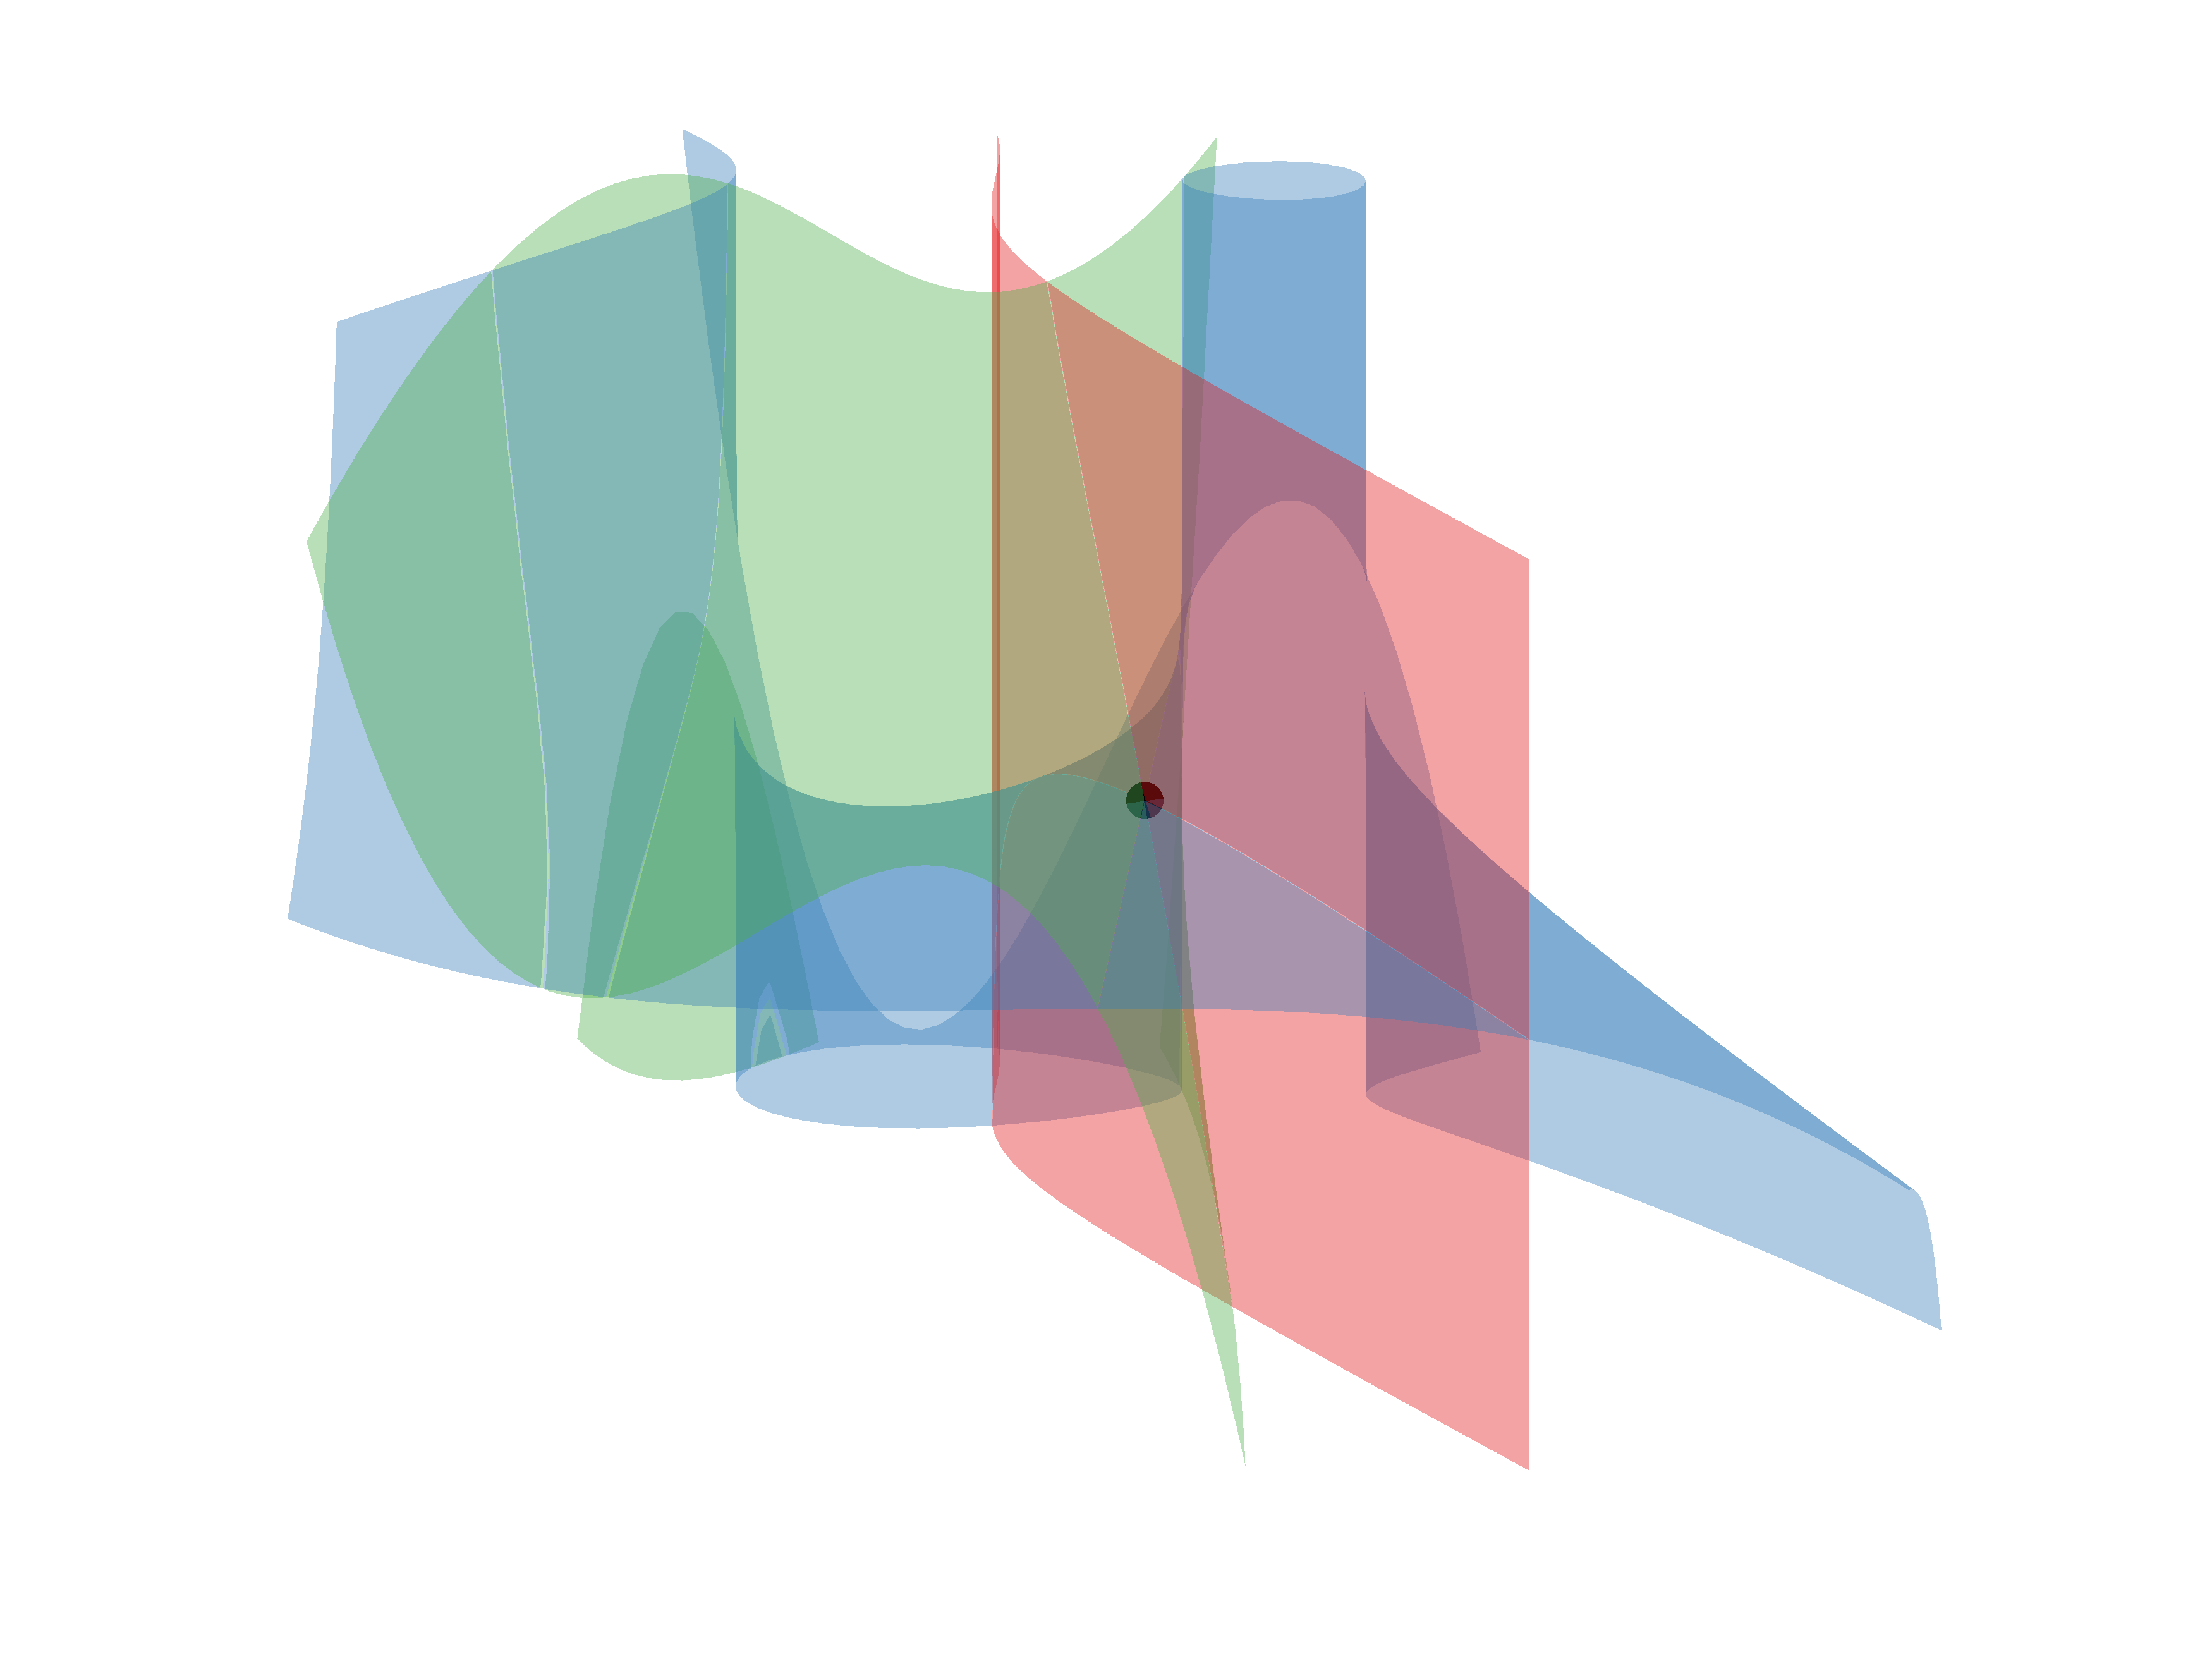
\includegraphics[width=0.8\textwidth]{"images/e3c3_example1.png"}
		\caption{Die drei kubischen Flächen zu Beispiel \ref{ex:3C3_1} und deren gemeinsamer Schnittpunkt.}
	\end{figure}
\end{example}
\begin{example}\label{ex:3C3_2}
	Betrachten wir das Gleichungssystem
	\begin{equation}\label{eqn:example3C3_2}
		\begin{alignedat}{1}
-\frac{4171\,x^3}{500}+\frac{8539\,y\,x^2}{1000}-\frac{1598\,y\,x}{125}-\frac{483\,z^3}{100}-\frac{2071\,z^2}{1000}-\frac{1113\,z}{125}-\frac{237}{20}&=0,\\ -\frac{3409\,x^3}{1000}+\frac{2331\,y\,x^2}{500}+\frac{2769\,y\,x}{500}-\frac{13419\,z^3}{1000}-\frac{207\,z^2}{500}-\frac{494\,z}{125}+\frac{2087}{500}&=0,\\ \frac{1141\,x^3}{125}-\frac{4277\,y\,x^2}{1000}+\frac{276\,y\,x}{125}+\frac{5443\,z^3}{500}+\frac{1339\,z^2}{250}+\frac{7797\,z}{1000}+\frac{7667}{1000}&=0
		\end{alignedat}
	\end{equation}
	über $\R$ so erhalten wir mit dem 3C3-Algorithmus die Lösung
	\begin{equation*}
		\begin{alignedat}{5}
			&\left( x_{1},y_{1},z_{1}\right) &=& \left(-1.455403524, -0.00005808002828, 0.9263500529 \right).&&
		\end{alignedat}
	\end{equation*}
\end{example}
\begin{figure}[H]
	\begin{subfigure}[b]{0.8\textwidth}
	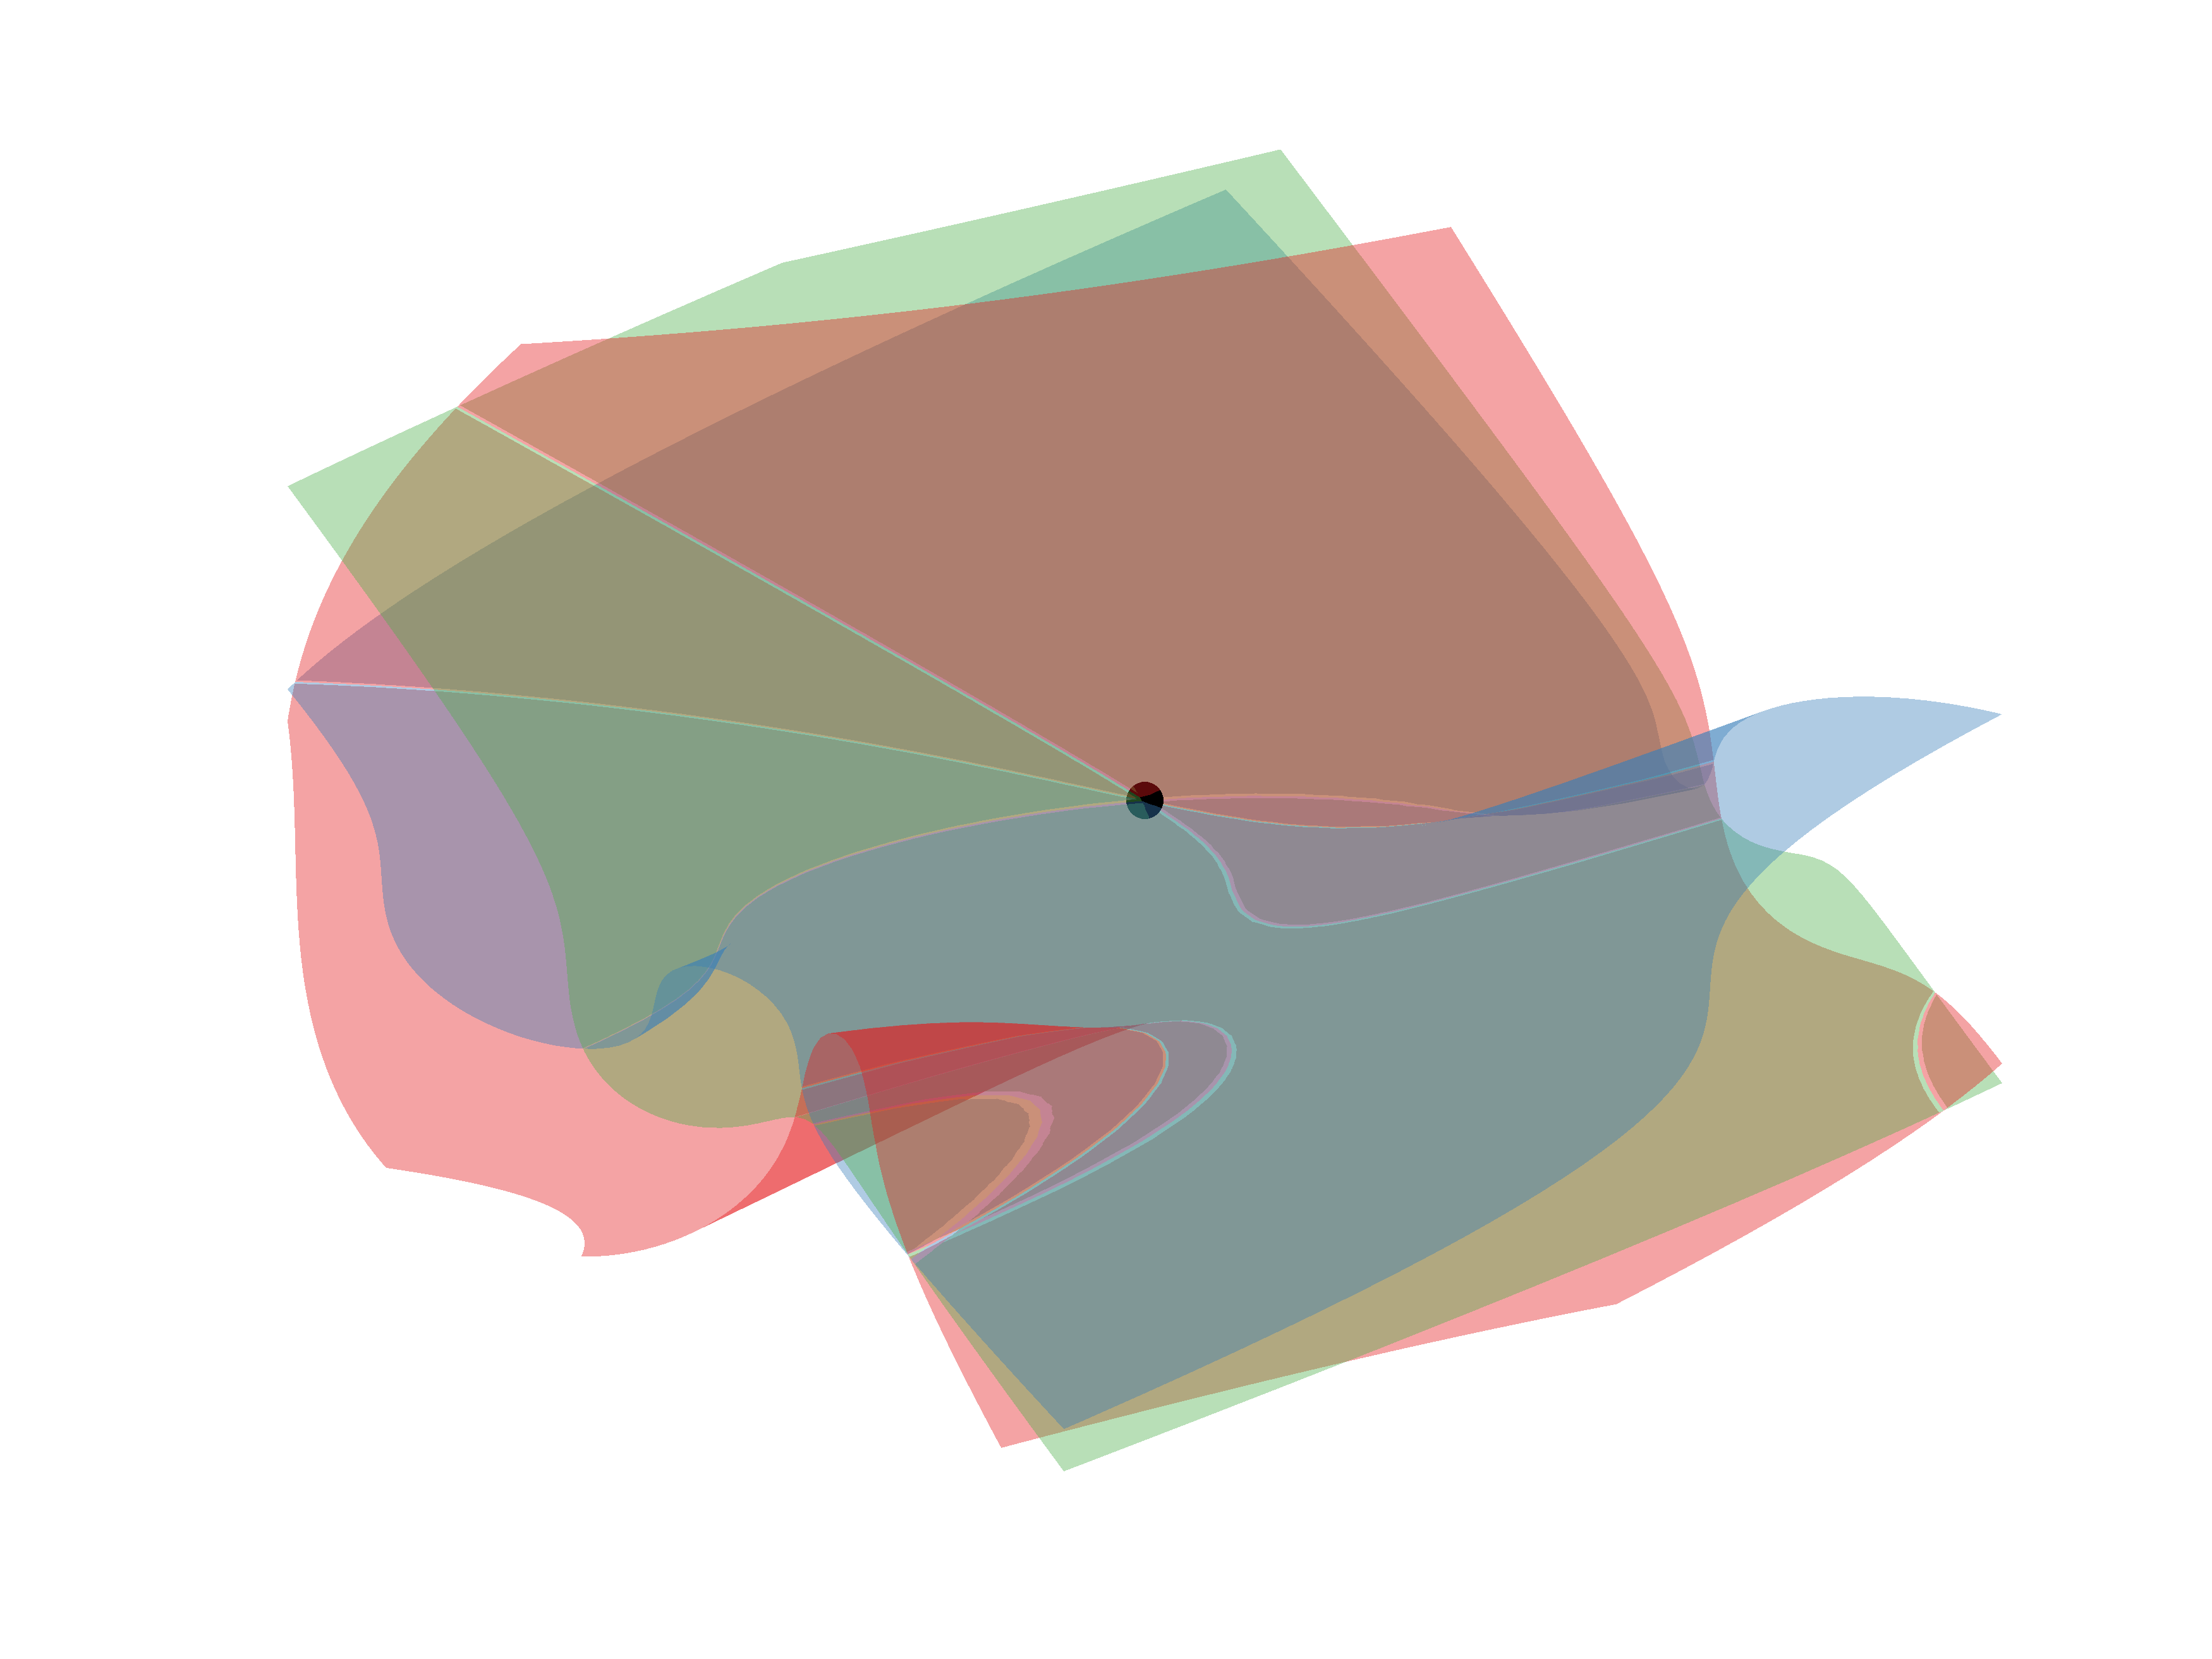
\includegraphics[width=\textwidth]{"images/e3c3_example2.png"}
	\caption{Die drei kubischen Flächen von System \eqref{eqn:example3C3_2} und deren gemeinsamer Schnittpunkt.}
\end{subfigure}
\end{figure}
\begin{figure}[H]\ContinuedFloat
	\begin{subfigure}[b]{0.8\textwidth}
	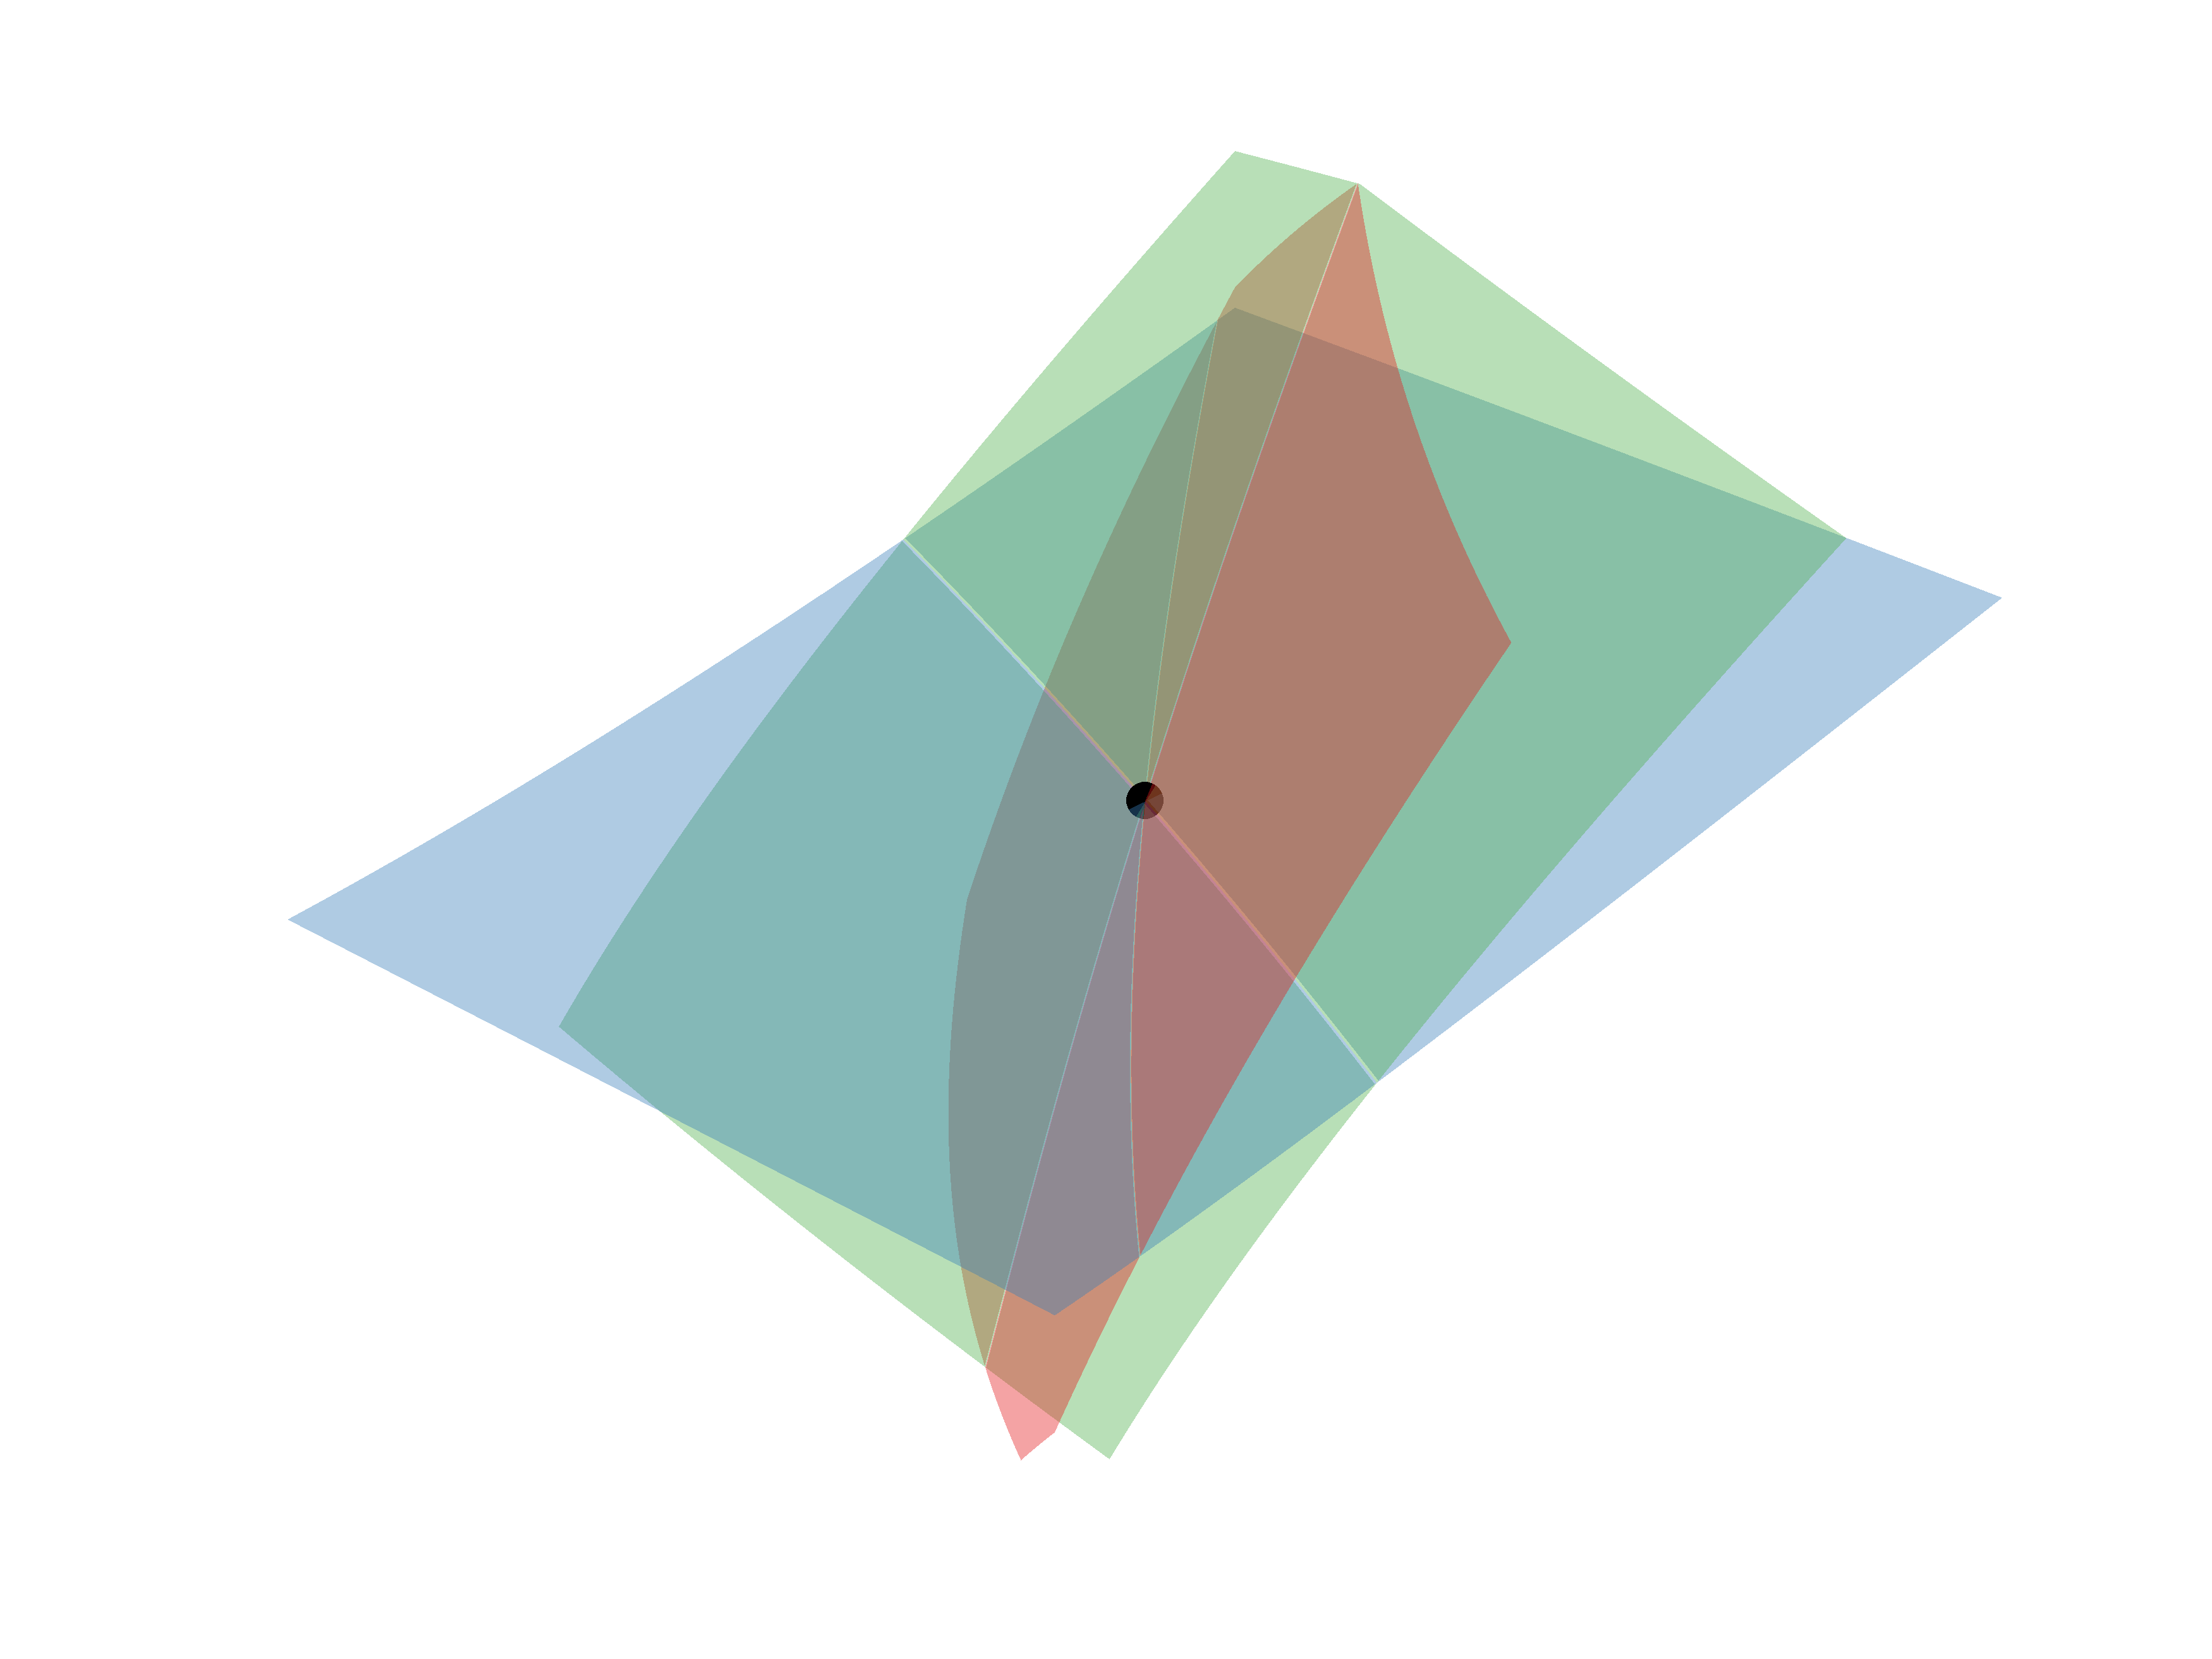
\includegraphics[width=\textwidth]{"images/e3c3_example2_zoom.png"}
	\caption{Die drei kubischen Flächen aus dem System \eqref{eqn:example3C3_2} in der nahen Umgebung ihres gemeinsamen Schnittpunktes.}
\end{subfigure}
\caption{Die Geometrie der kubischen Flächen aus Beispiel \ref{ex:3C3_2}.}
\end{figure}
\begin{example}\label{ex:3C3_3}
	Betrachten wir das Gleichungssystem
	\begin{equation}\label{eqn:example3C3_3}
		\begin{alignedat}{1}
			5\,x^3-5\,z^3+3\,z^2+14\,z+12&=0\\ 3\,y\,x^2+9\,z^3+8\,z^2-9\,z-7&=0\\ 8\,z^3-8\,z^2-12\,z+x\,y+10&=0,
		\end{alignedat}
	\end{equation}
	über $\R$ so erhalten wir mit dem 3C3-Algorithmus die Lösung
	\begin{equation*}
		\begin{alignedat}{5}
			&\left( x_{1},y_{1},z_{1}\right) &=& \left(-1.16125,-0.000354396,-1.17694 \right).&&
		\end{alignedat}
	\end{equation*}
\end{example}
\begin{figure}[H]
	\begin{subfigure}[b]{0.8\textwidth}
	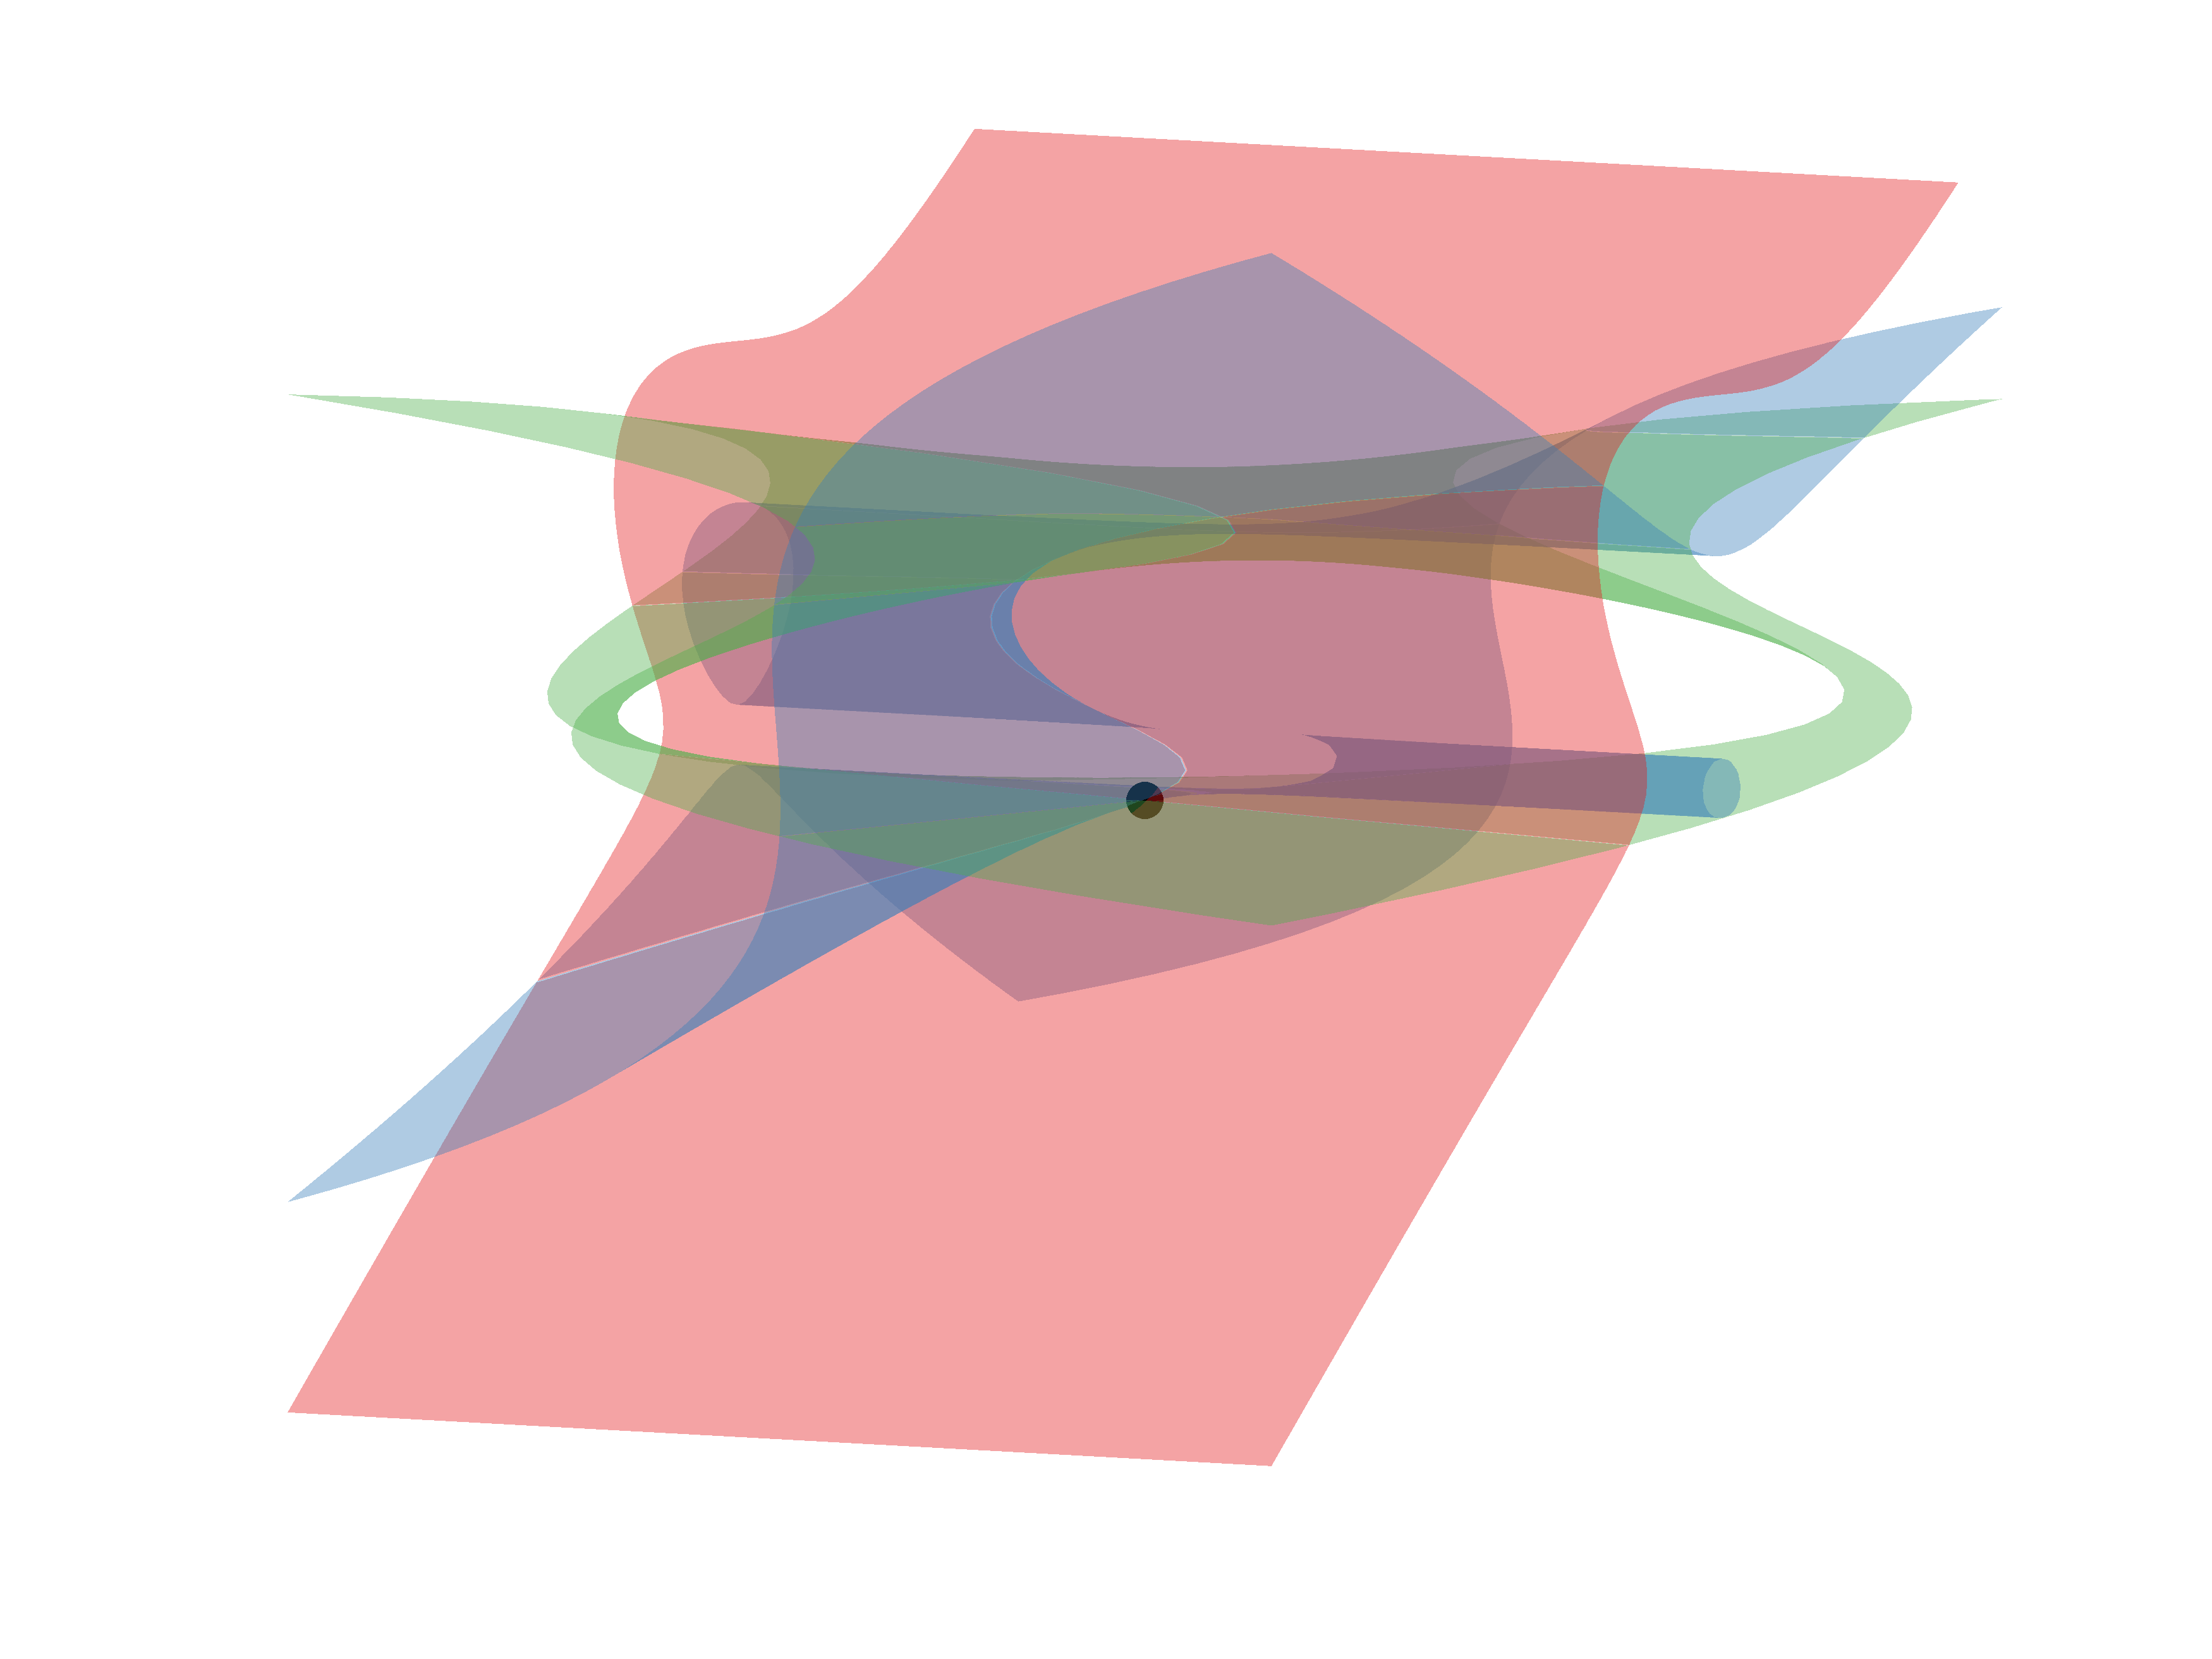
\includegraphics[width=\textwidth]{"images/e3c3_example3.png"}
	\caption{Die drei kubischen Flächen des Systems \eqref{eqn:example3C3_3} und deren gemeinsamer Schnittpunkt.}
\end{subfigure}
\end{figure}
\begin{figure}[H]\ContinuedFloat
	\begin{subfigure}[b]{0.8\textwidth}
	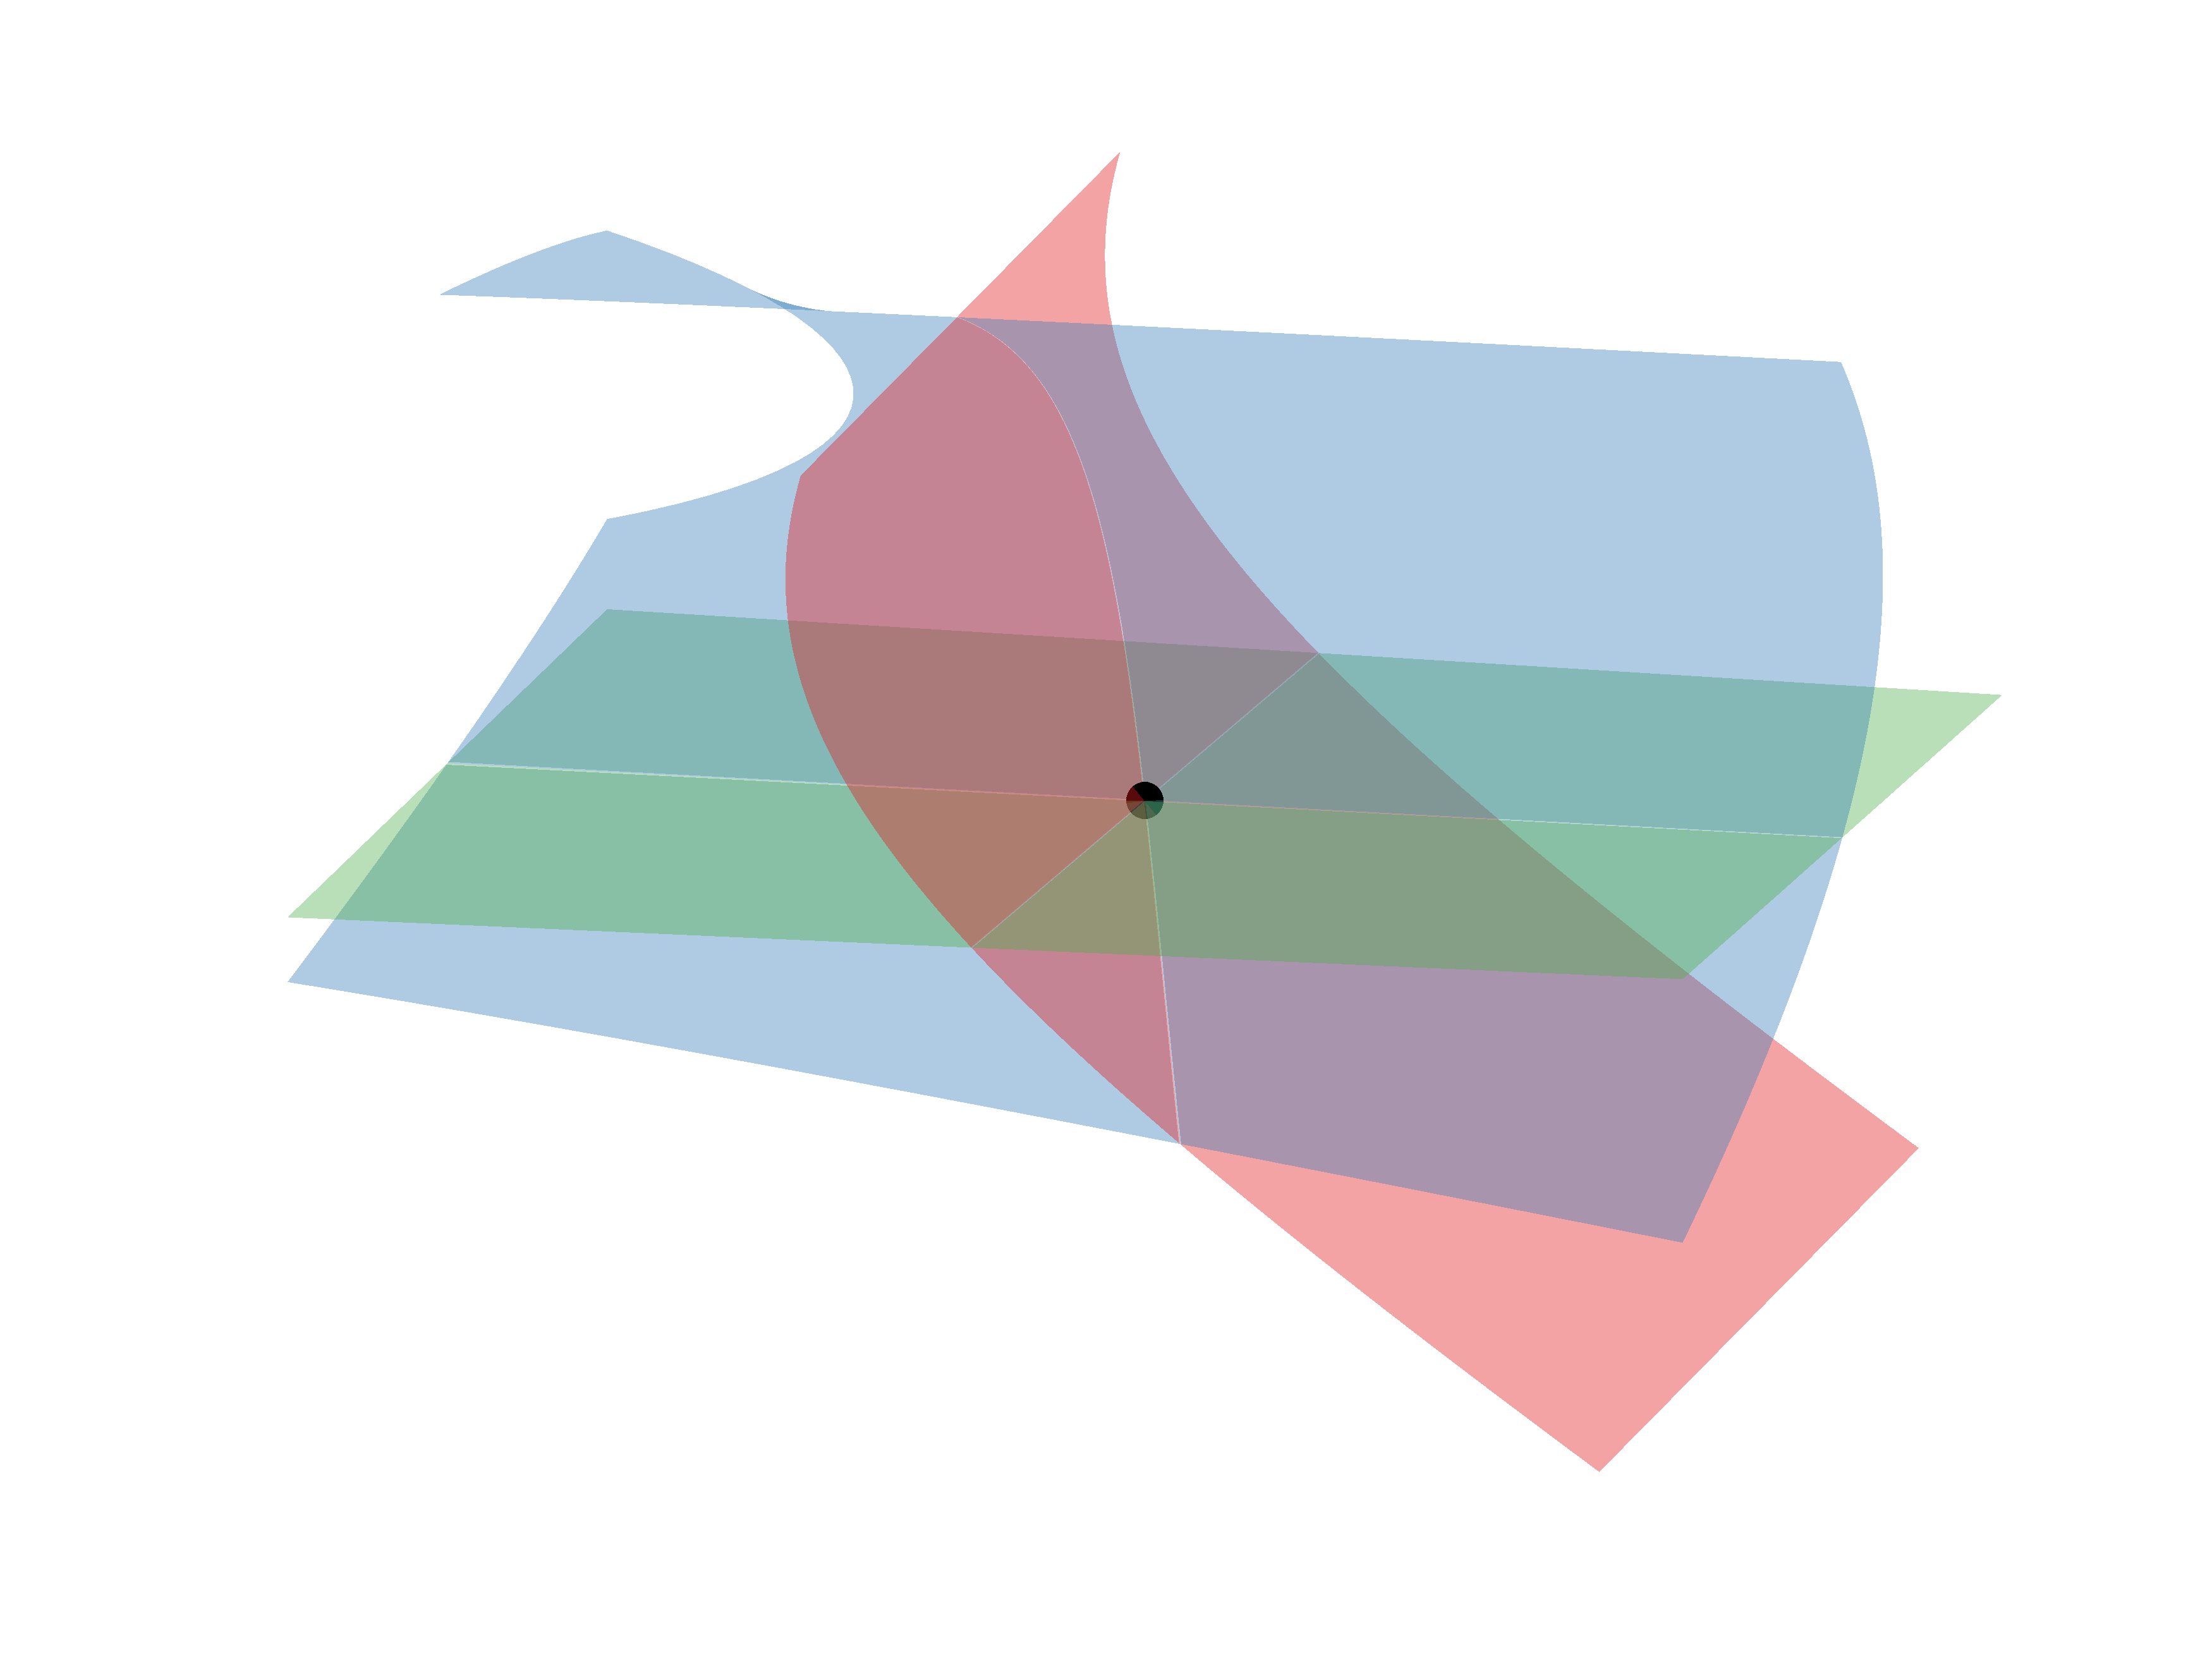
\includegraphics[width=\textwidth]{"images/e3c3_example3_zoom.png"}
	\caption{Die drei kubischen Flächen aus dem System \eqref{eqn:example3C3_3} in der nahen Umgebung ihres gemeinsamen Schnittpunktes.}
\end{subfigure}
\caption{Die Geometrie der kubischen Flächen aus Beispiel \ref{ex:3C3_3}.}
\end{figure}
\begin{example}
	Betrachten wir das Gleichungssystem
	\begin{equation}
		\begin{alignedat}{1}
			4\,z\,x^2+6\,z\,x+7\,y^3+2\,y^2+4\,y+7&=0\\ -x^3+2\,z\,x^2-4\,z\,x+4\,y^3+10\,y^2+5\,y-2&=0\\ 7\,z\,x^2+2\,z\,x+8\,y^3-3\,y^2-3&=0
		\end{alignedat}
	\end{equation}
	über $\F{13}$ so erhalten wir mit dem 3C3-Algorithmus die Lösungen
	\begin{equation*}
	\begin{alignedat}{5}
		&\left( x_{1},y_{1},z_{1}\right) &=& \left(12,1,10 \right),&&\\
		&\left( x_{2},y_{2},z_{2}\right) &=& \left(3,8,3 \right)&& \quad\text{und} \\
		&\left( x_{3},y_{3},z_{3}\right) &=& \left(11,6,9 \right).&&
	\end{alignedat}
\end{equation*}
\end{example}
\begin{example}
	Betrachten wir das Gleichungssystem
	\begin{equation}
		\begin{alignedat}{1}
			121\,x^3+136\,z\,x^2+143\,z\,x+41\,y^3+142\,y^2+21\,y+118&=0\\ 134\,x^3+94\,z\,x^2+23\,z\,x+81\,y^3+72\,y^2+62\,y+142&=0\\ 18\,x^3+14\,z\,x^2+144\,z\,x+142\,y^3+119\,y^2+136\,y+97&=0
		\end{alignedat}
	\end{equation}
	über $\F{149}$ so erhalten wir mit dem 3C3-Algorithmus die Lösung
	\begin{equation*}
		\begin{alignedat}{5}
			&\left( x_{1},y_{1},z_{1}\right) &=& \left(140,85,11 \right).&&
		\end{alignedat}
	\end{equation*}
\end{example}
\begin{example}
	Betrachten wir das Gleichungssystem
	\begin{equation}
		\begin{alignedat}{1}
2\,x^3+x-y^3+2&=0\\
 2\,x^3+2\,x^2+2\,x-z\,y^2+2&=0\\
  x^3+2\,x^2+3\,x-y\,z+3&=0
		\end{alignedat}
	\end{equation}
	über $\F{5}$ so erhalten wir mit dem 3C3-Algorithmus für die Lösung $x_1=2$ die Nullmatrix.
	In diesem Fall sind
	\begin{equation*}
		\begin{alignedat}{5}
			&\left( x_{1},y_{1},z_{1}\right) &=& \left(2,0,0 \right),&&\\
			&\left( x_{1},y_{1},z_{1}\right) &=& \left(2,0,1 \right),&&\\
			&\left( x_{1},y_{1},z_{1}\right) &=& \left(2,0,2 \right),&&\\
			&\left( x_{2},y_{2},z_{2}\right) &=& \left(2,0,3 \right)&& \quad\text{und} \\
			&\left( x_{3},y_{3},z_{3}\right) &=& \left(2,0,4 \right)&&
		\end{alignedat}
	\end{equation*}
	die Lösungen des Gleichungssystems.
\end{example}
\newpage


\section{Implementierung in MATLAB}\label{sec:matlab}
\subsection{Allgemeine Programmstruktur}
		Da die E3Q3, 3C3, 4C3 und 5C3 Algorithmen alle nach dem gleichen Prinzip verfahren, sind auch die Programmstrukturen der Implementierungen in MATLAB gleich.
		\begin{figure}[H]
		\centering
		\begin{tikzpicture}[scale=0.05,>=latex',
			block/.style = {draw, shape=rectangle, align=center},
			rblock/.style = {draw, shape=rectangle, rounded corners=0.5em},
			tblock/.style = {draw, shape=trapezium, trapezium left angle=60, 
				trapezium right angle=120, align=center},
			diamond/.style = {draw, shape=diamond, align=center,aspect=2},
			subprg/.style = {draw, shape=rectangle split,rectangle split parts=3, align=center}
			]
			\node [tblock] (input) {Eingabe der Koeffizientenmatrix};
			\node [subprg,rectangle split horizontal, below=of input]       (split)   {\nodepart{two} split\_matrices};
			\node [subprg,rectangle split horizontal, below=of split]       (subs)   {\nodepart{two} substitute\_identities};
			\node [block, below=1cm of subs]       (detM)   {Berechne $\det\left( M\left(X_i \right)\right) $};
			\node [block, below=0.5cm of detM] (sturm)   {Berechne symbolische Nullstellen $\tilde{x}_i$};
			\node [tblock, right=2cm of sturm, align=center] (noresults) {Keine Lösung};
			\node [block, below=0.5cm of sturm] (subsM) {Setze Lösung $\tilde{x}_i$ in $M$ ein};
			\node [subprg,rectangle split horizontal, below=0.5cm of subsM] (solve) {\nodepart{two} solve\_subsystem};
			\node [diamond, below=0.5cm of solve] (fin) {Alle $\tilde{x}_i$ durchgegangen?};
			\node [coordinate,right=1cm of fin] (a) {};
			\node [coordinate,right=1cm of subsM] (b) {};
			\draw[->] (input) -- (split);
			\draw[->] (split) -- (subs);
			\draw[->] (subs) --node[pos=0.5,anchor=west,align=center]{Matrix $M(X_i)$} (detM);
			\draw[->] (detM) -- (sturm);
			\draw[->] (sturm) --node[pos=0.5,anchor=south,align=center]{Keine\\Nullstellen} (noresults);
			\draw[->] (sturm) -- (subsM);
			\draw[->] (subsM) -- (solve);
			\draw[->] (solve) -- (fin);
			\draw[->] (fin) --node[pos=0.4,anchor=south]{Nein} (a) |-node[pos=0.25,anchor=west]{Wähle nächste Nullstelle} (b) -- (subsM);
			\node [subprg,rectangle split horizontal, below=0.5cm of fin] (plot) {\nodepart{two} plot\_and\_color};
			\draw[->] (fin) -- (plot);
			\node [tblock, below=0.5cm of plot] (output) {Ausgabe der Lösungen};
			\draw[->] (plot) -- (output);
			%etc
		\end{tikzpicture}
		\caption{Allgemeiner Programmaufbau der Hauptprogramme in MATLAB}
	\end{figure}
	
	Im E3Q3 und 5C3-Algorithmus erfolgt die Wahl der Unbestimmten, welche in den Koeffizientenbereich gesetzt wird, dadurch, dass für jede der Unbestimmten die Matrix $C$ bestimmt wird und diejenige mit der niedrigsten Konditionszahl wird verwendet. Bei den Implementierung für endliche Körper hingegen werden die Matrizen nacheinander berechnet und die erste invertierbare Matrix wird verwendet.
	
	In den 3C3 und 4C3 Algorithmen werden alle Matrixaufteilungen nacheinander berechnet. Die erste Unbestimmte, deren Matrix $P$ die Vorraussetzungen erfüllt, wird dann für den Algorithmus gewählt.\\
	Der 3C3-Algorithmus mit $G_1=\{X_2^3,X_2^2X_3,X_2X_3^2\}$ wurde im Rahmen dieser Arbeit nicht implementiert.
	
	Die Plots für den E3Q3-Algorithmus werden durch Parametrisierungen der Quadriken erstellt, während für die  Visualisierungen der kubischen Flächen implizite Plotfunktionen verwendet werden.
	
	Da MATLAB nur sehr limitierte Rechenmöglichkeiten in Primkörpern $\F{p}$ besitzt, führen wir alle Berechnungen mithilfe der Klasse \glqq FF.m\grqq~ aus. In dieser Klasse sind neben den Standardoperationen $+$, $\cdot$, $-$ und $/$, alle symbolischen Manipulationen, sowie weitere Funktionen für Matrizen über endlichen Körpern implementiert.\\
	Für den E3Q3-Algorithmus und den 5C3-Algorithmus werden alle Fallunterscheidungen für die Matrix $\text{rref}(\tilde{M})$ durch entsprechende Unterprogramme gelöst. Für die 4C3 und 3C3 Algorithmen sind aus Zeitgründen nur die Fälle für $\text{rank}(\tilde{M}) \geq 3$ implementiert, da der Fall $\text{rank}(\tilde{M}) \leq 2$ nicht auftrat.
	\newpage
	\subsection{Laufzeitvergleich und Grenzen der Implementierungen}
	Natürlich stellt sich die Frage, wie ein einfaches Durchgehen aller Möglichkeiten gegenüber dem E3Q3-Algorithmus und dem 3C3-Algorithmus abschneidet.
	Der E3Q3-Algorithmus ist bis zur Größenordnung $p \geq 150$ dem naiven Ansatz unterlegen, jedoch steigt die Laufzeit des naiven Ansatzes kubisch zu Ordnung des Körpers $\F{p}$. Die Laufzeit des E3Q3-Algorithmus steigt im Vergleich nur langsam mit der Ordnung $p$ an.
	\begin{figure}[H]
		\begin{subfigure}[b]{0.7\textwidth}
			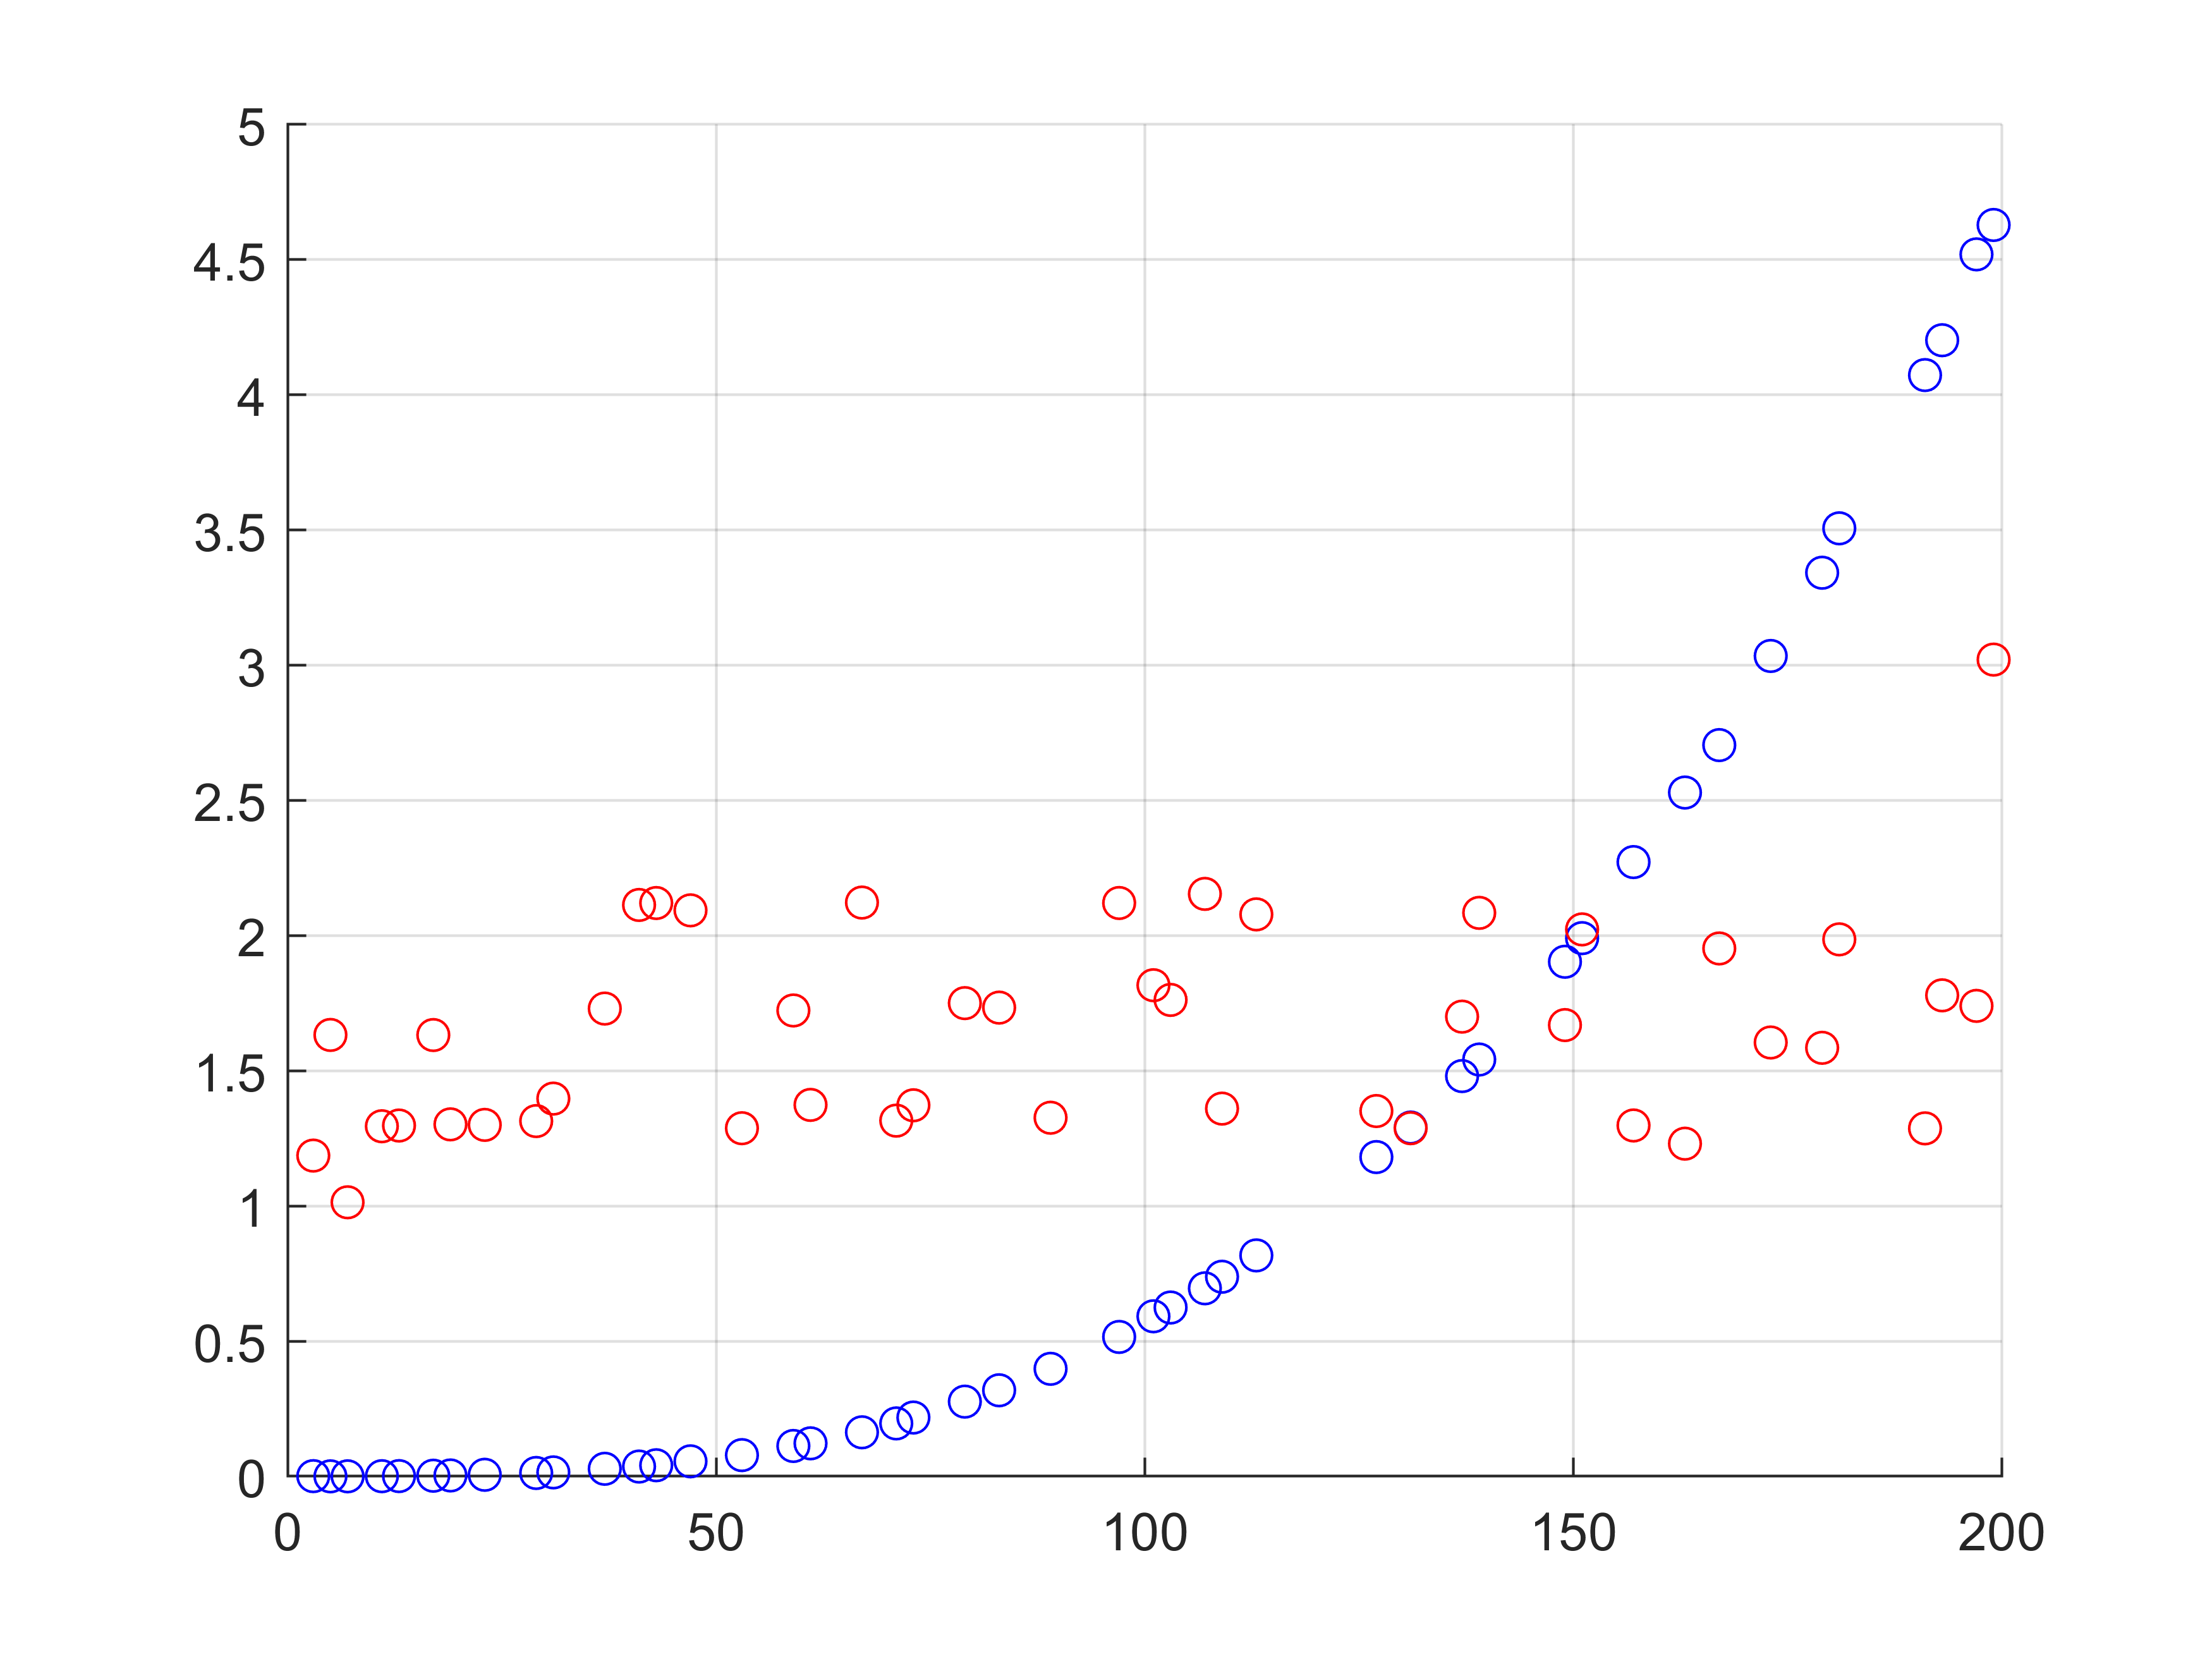
\includegraphics[width=\textwidth]{"images/runtime_e3q3_for_loop.png"}
		\end{subfigure}
			\caption{Die Mittelwerte der Programmlaufzeiten des E3Q3-Algorithmus (rot) über Körpern $\F{p}$ verglichen mit der Iteration über alle Elemente in $\F{p}^3$ (blau).}
	\end{figure}
	Die Implementierung des E3Q3-Algorithmus wurde stichprobenartig für Körper mit über $10^6$ Elementen erfolgreich getestet. Für höhere Größenordnungen stößt die MATLAB jedoch an seine Grenzen das Programm stürzt ab.
	\begin{figure}[H]\label{fig:e3q3_runtime}
		\begin{subfigure}[b]{0.7\textwidth}
			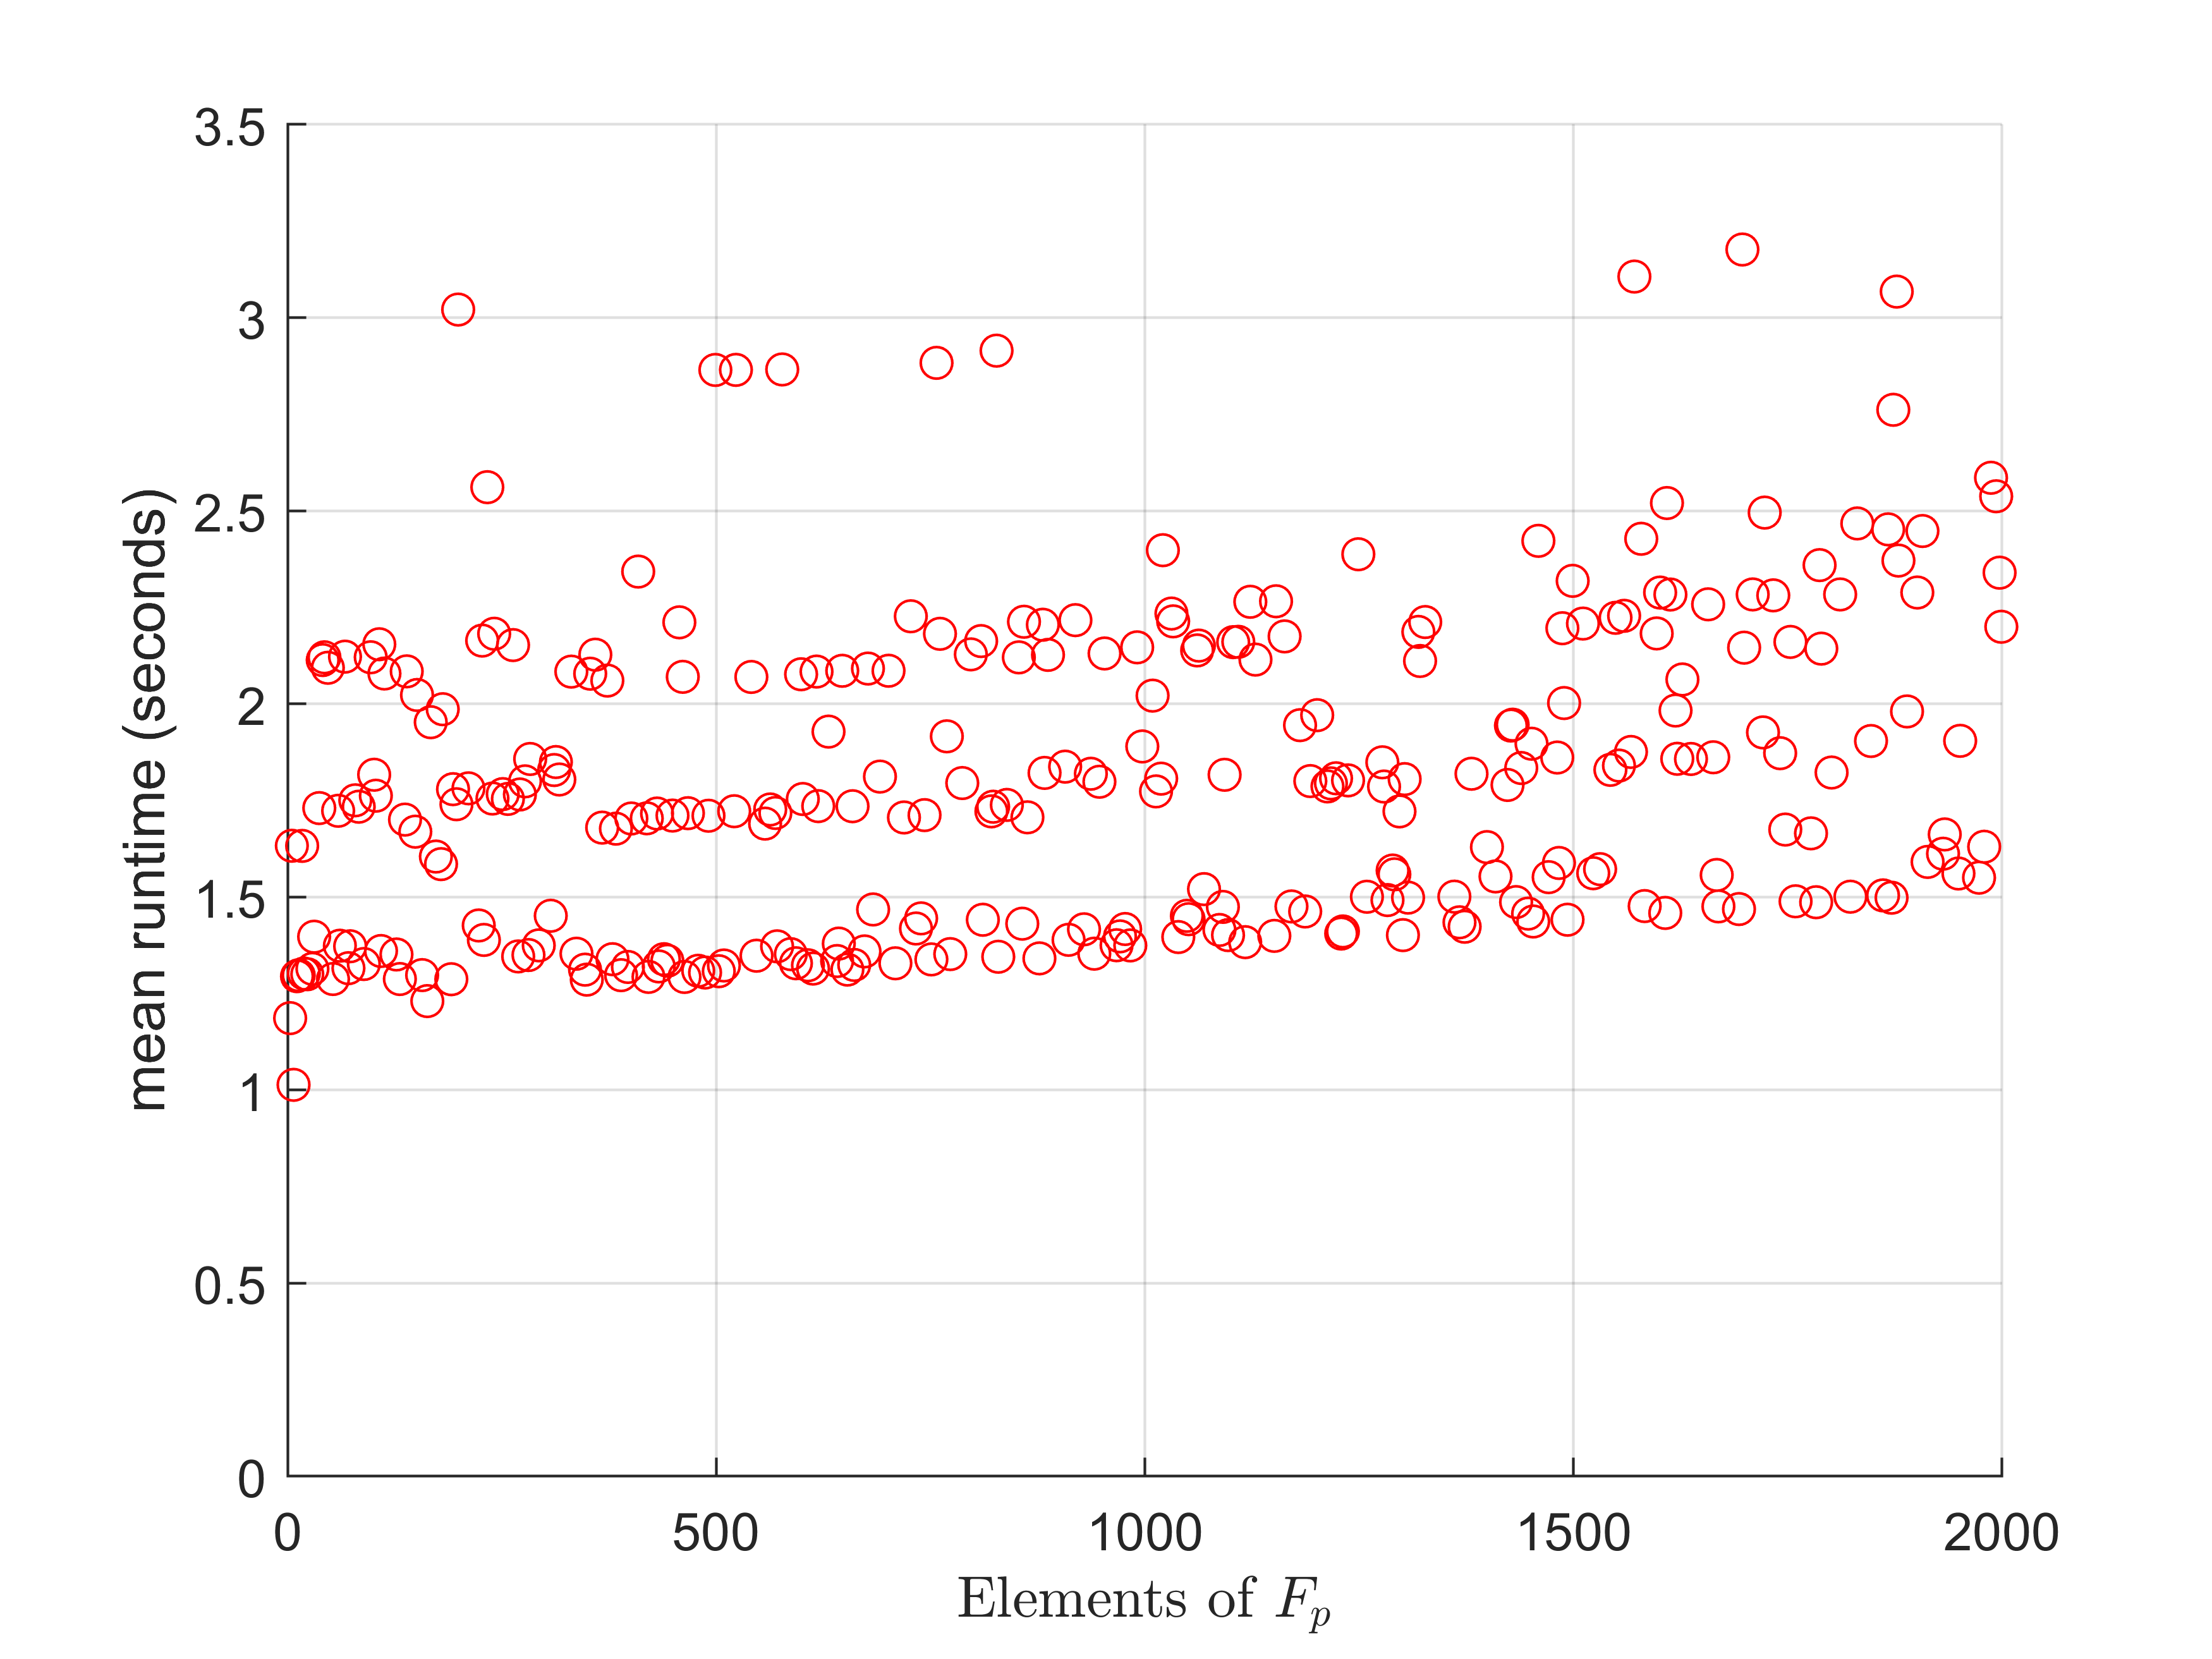
\includegraphics[width=\textwidth]{"images/runtime_e3q3.png"}
		\end{subfigure}
		\caption{Die Mittelwerte der Programmlaufzeiten des E3Q3-Algorithmus über Körpern $\F{p}$.}
	\end{figure}
	Der 3C3-Algorithmus ist bis zur Größenordnung $p \geq 150$ langsamer als der naive Ansatz, für größere Körper $\F{P}$ ist er jedoch deutlich schneller.
	\begin{figure}[H]
		\begin{subfigure}[b]{0.7\textwidth}
			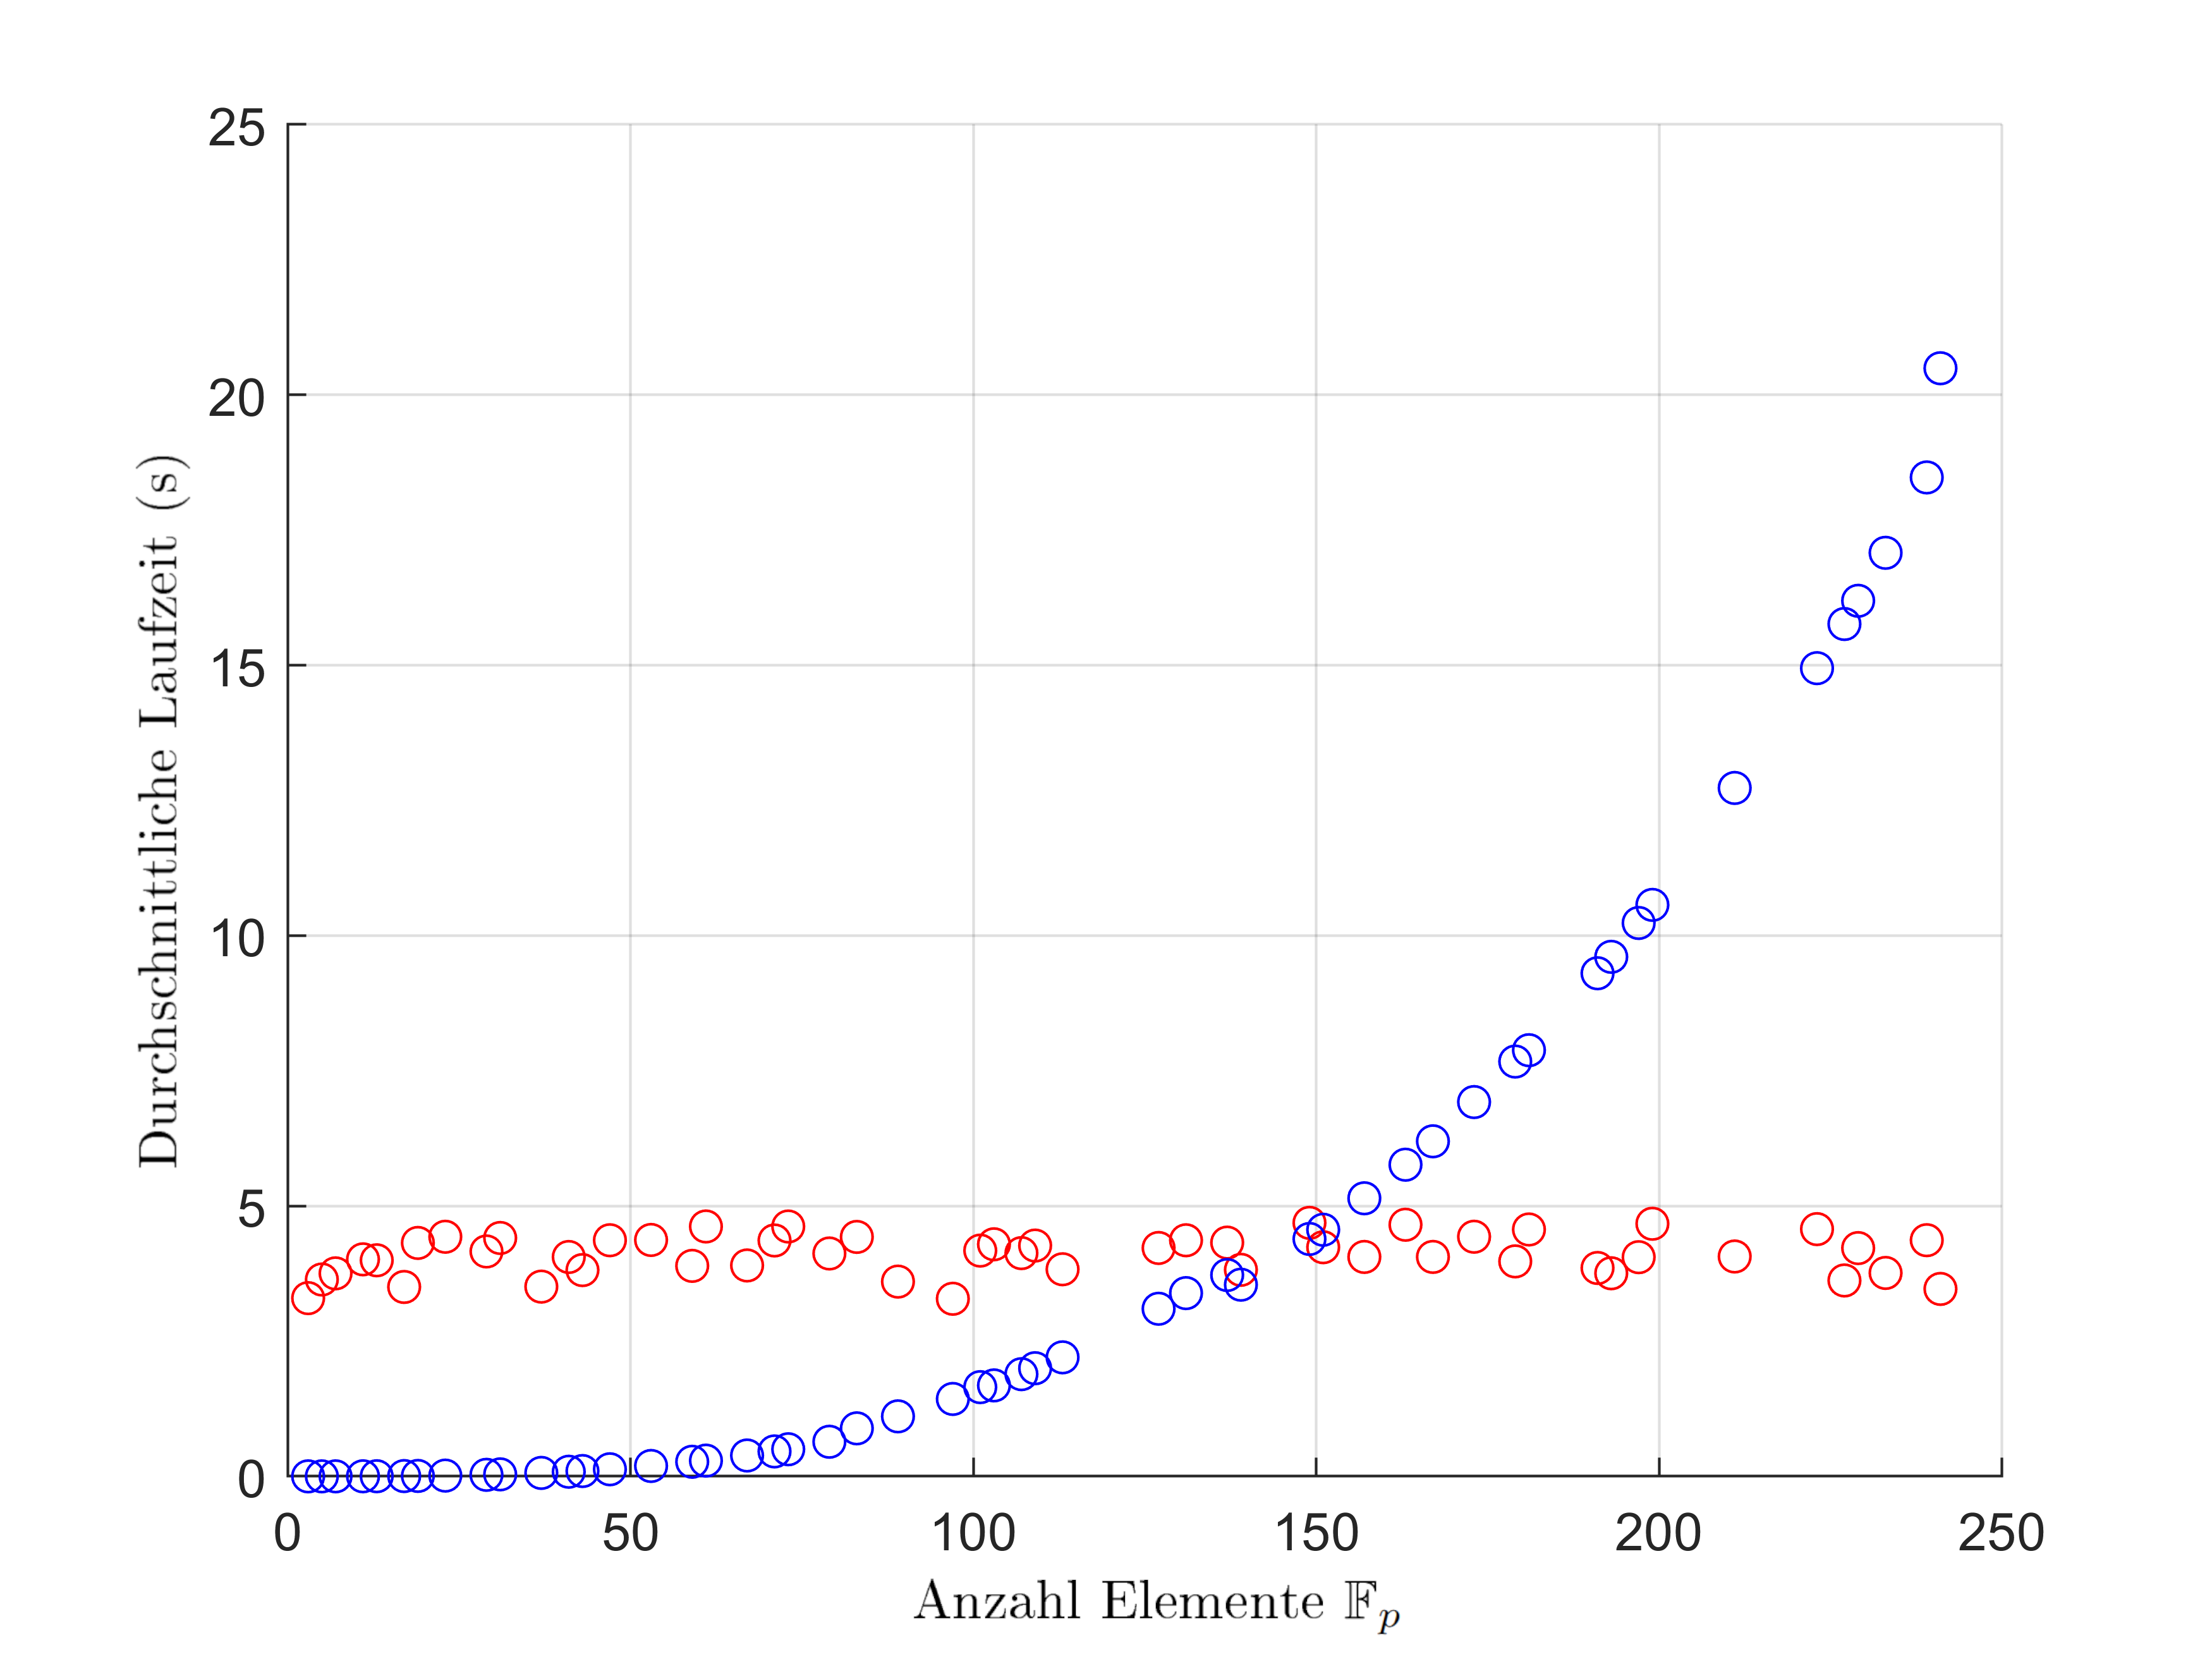
\includegraphics[width=\textwidth]{"images/runtime_e3c3_for_loop.png"}
		\end{subfigure}
		\caption{Die Mittelwerte der Programmlaufzeiten des 3C3-Algorithmus (rot) über Körpern $\F{p}$ verglichen mit der Iteration über alle Elemente in $\F{p}^3$ (blau).}
	\end{figure}
	\newpage
	Bei den Laufzeiten des 3C3-Algorithmus fällt jedoch auf, dass diese ab $p=270$ abfallen.
	Dies liegt daran, dass der Algorithmus ab dieser Größenordnung immer mehr numerische Fehler auftreten, welche dazu führen, dass der Algorithmus Schritte überspringt und keine Lösungen findet. Diese Fehler könnte man mit einer besseren Implementierung des Rechnens über $\F{p}$ in MATLAB oder durch die Implementierung in einer anderen Programmiersprache behoben werden.
	\begin{figure}[H]\label{fig:e3c3_runtime}
		\begin{subfigure}[b]{0.7\textwidth}
			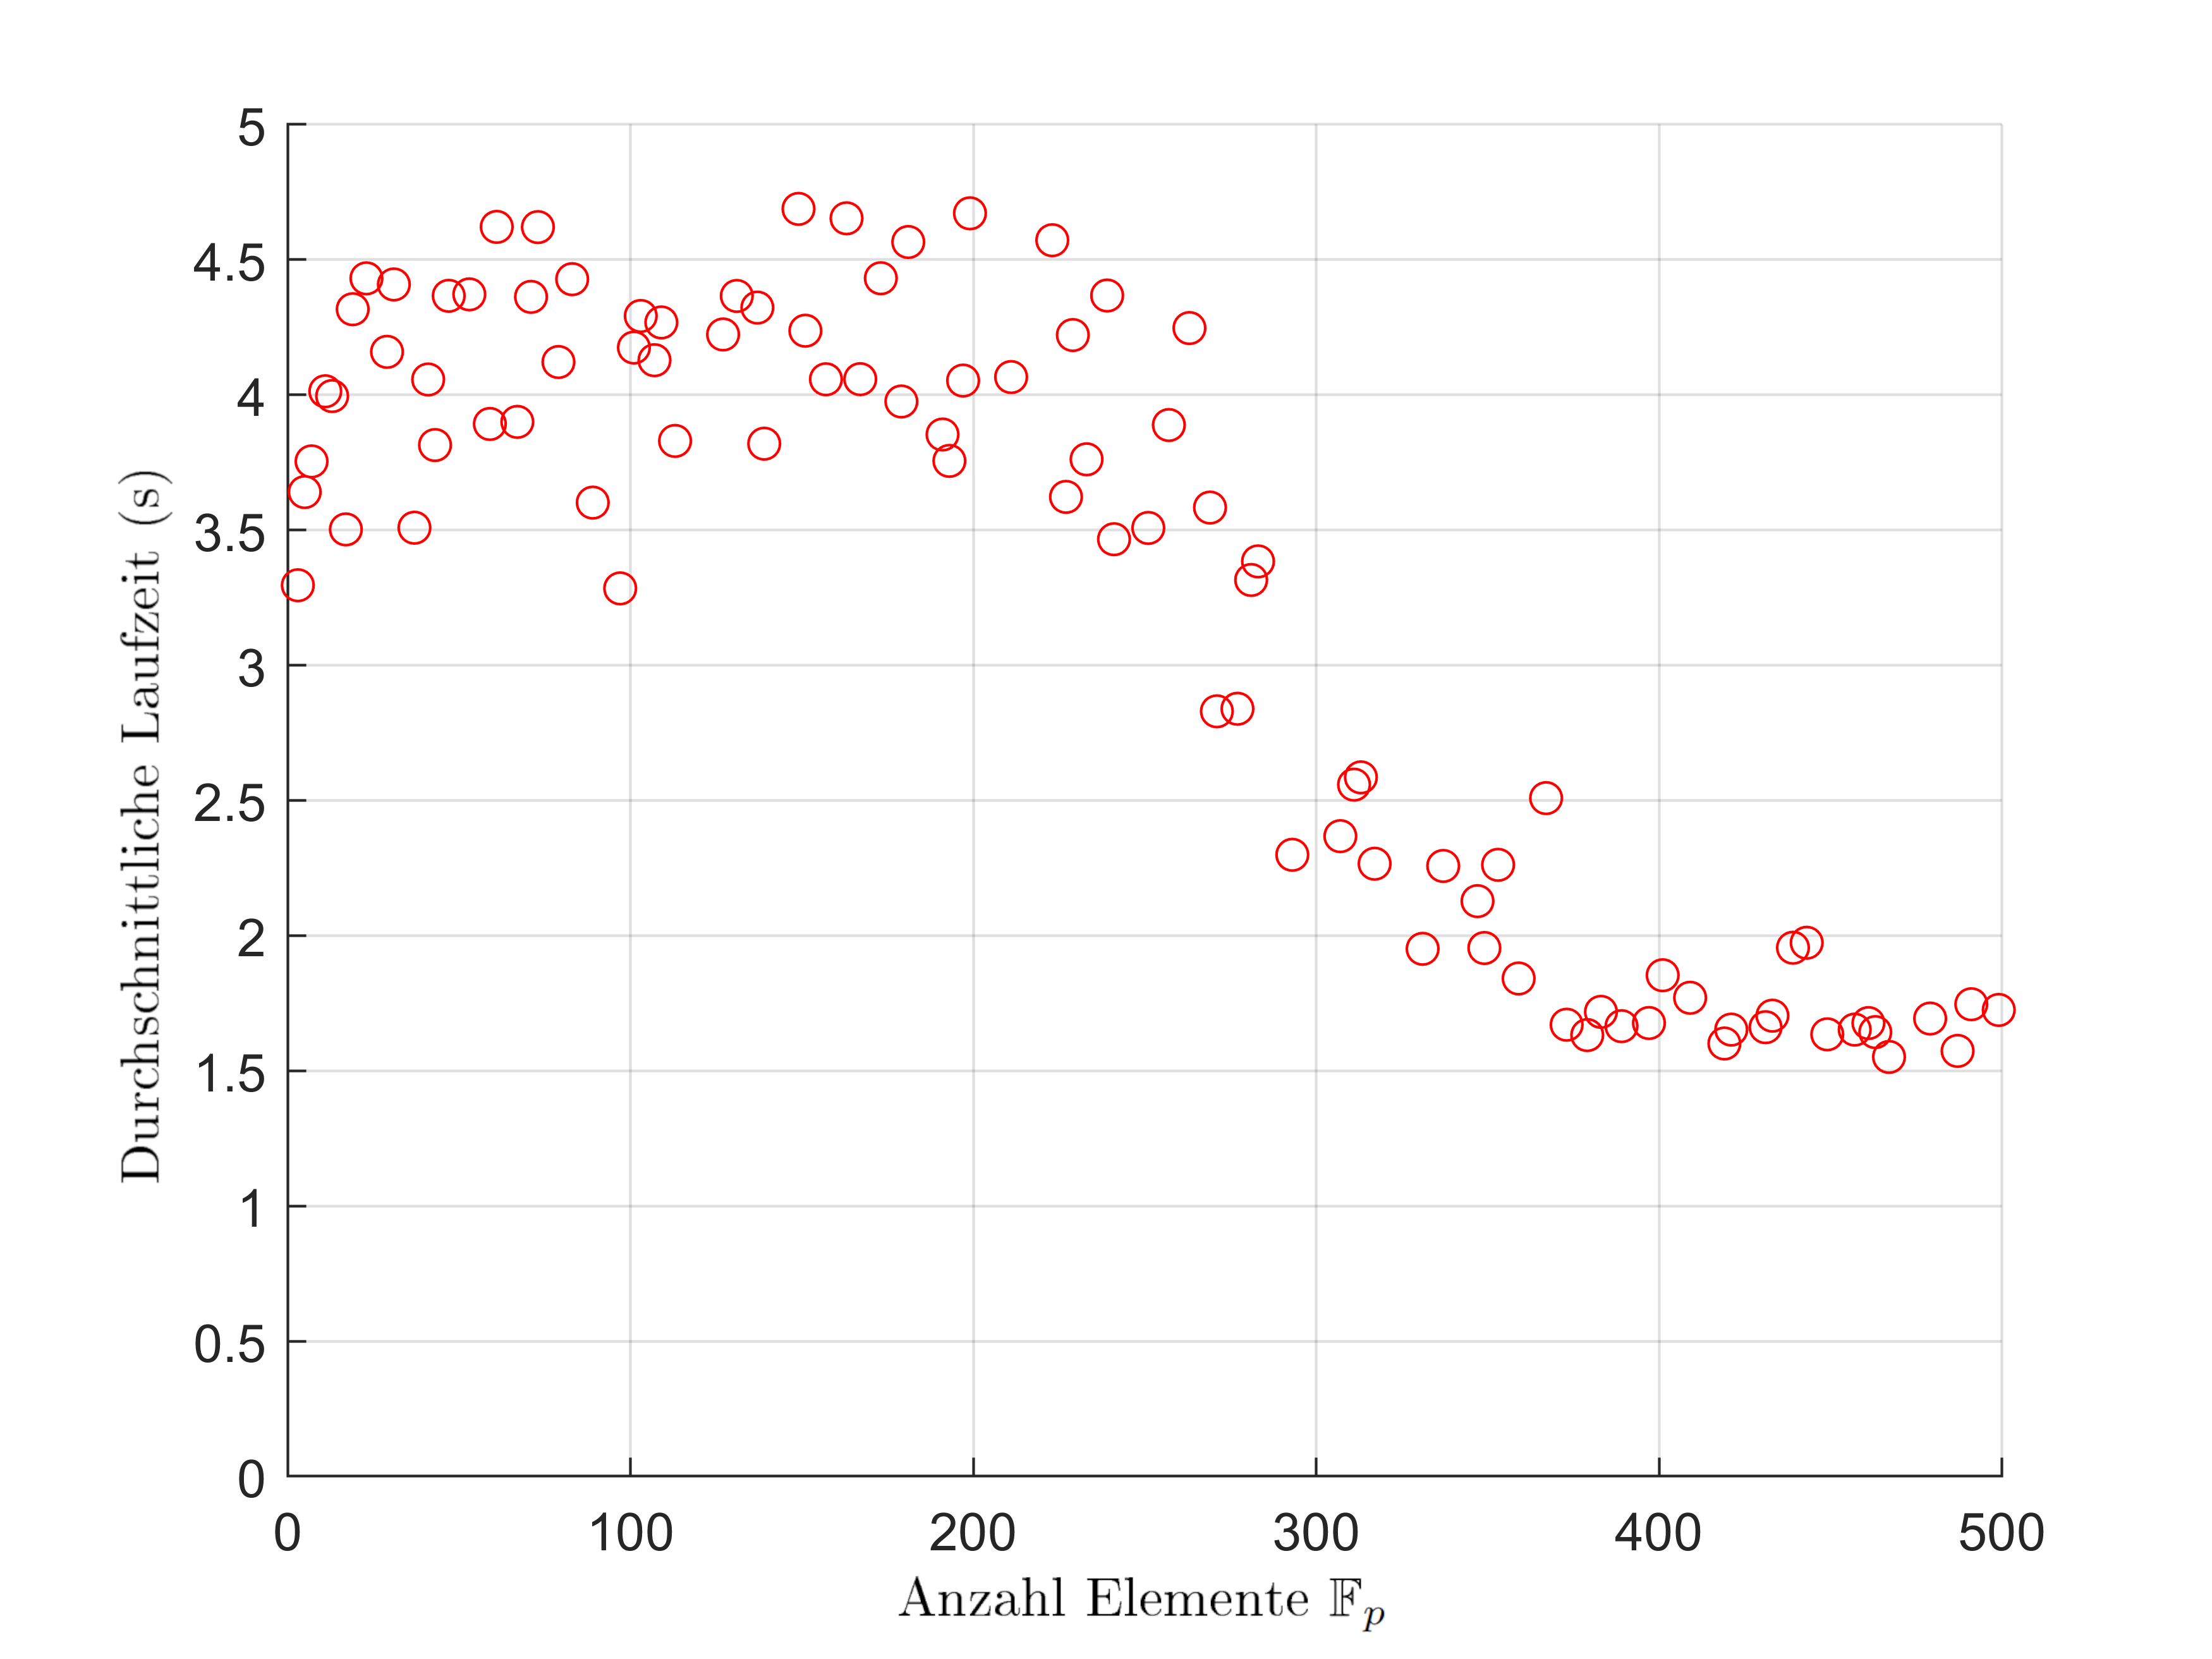
\includegraphics[width=\textwidth]{"images/runtime_e3c3.png"}
		\end{subfigure}
		\caption{Die Mittelwerte der Programmlaufzeiten des 3C3-Algorithmus über Körpern $\F{p}$.}
	\end{figure}
	\newpage
	\section{Fazit, Ausblick, offene Fragestellungen}\label{sec:fazit}
	\subsection*{Fazit}
In dieser Arbeit haben wir erfolgreich den E3Q3-Algorithmus über $\R$ und für endliche Primkörper formuliert und in MATLAB implementiert. Die Verallgemeinerung auf kubische Gleichungssysteme führte uns, über eine symmetrische Aufteilung der Monome, zuerst zu einem 5C3-Algorithmus zur Lösung doppelt überbestimmter Gleichungssysteme aus kubischen Polynomen in drei Unbestimmten. Schrittweise haben wir diesen Ansatz, mit Voraussetzungen an das Gleichungssystem, zunächst auf einfach überbestimmte Gleichungssysteme (4C3) und mit noch strengeren Anforderungen auf den ursprünglich gesuchten 3C3-Algorithmus angewendet, welcher die gleiche Anzahl an Gleichungen und Unbestimmten als Ausgangspunkt hat. Alle drei Algorithmen konnten wir in MATLAB sowohl für reelle Zahlen als auch endliche Körper implementieren, wobei diese im Falle des 3C3-Algorithmus schon für recht kleine Ordnungen $p$ fehleranfällig sind. Im Gegensatz dazu funktioniert der E3Q3-Algorithmus für Größenordnungen bis zu $10^6$ und liefert die richtigen Lösungen.
	
	\subsection*{Offene Fragestellungen}
	Wie bereits in Abschnitt \ref{sec:3C3_alg} geschrieben, kann es sein, dass im 3C3-Algorithmus die Nullmatrix auftaucht. In den anderen Algorithmen korrespondierte dies damit, dass der Lösungskandidat $\tilde{x}_1$ keine Lösung war. Im 3C3-Algorithmus führt dies aber zu dass jedes Element der Menge \begin{equation*}
		\{(\tilde{x}_i,0,z) \ \forall z \in K\}
	\end{equation*}
	eine Lösung ist. Hier ist nicht klar, ob aus dem Auftreten der Nullmatrix immer diese Lösungsmenge folgt.
	Auch könnte es neben $G_1=\{X_2^3,X_2^2X_3,X_2X_3\}$ und $G_1=\{X_2^3,X_2^2X_3,X_2X_3^2\}$ noch weitere Aufteilungen der Monome in $G_1$ und $G_2$ geben, für welche sich passende Identitäten für einen 3C3-Algorithmus formulieren lassen.
	Der 3C3-Algorithmus mit  $G_1=\{X_2^3,X_2^2X_3,X_2X_3^2\}$ wurde in dieser Arbeit nicht implementiert oder genauer untersucht.
	\newpage
	\pagestyle{plain}

	\nocite{*}
	\bibliography{bibliography.bib}
			\newpage
	\section*{Danksagung}
	\pagenumbering{gobble}
	Nach sechs Jahren des intensiven Studiums an der Hochschule RheinMain im Studiengang Angewandte Mathematik ist der Moment gekommen, Abschied zu nehmen und auf diese prägende Zeit zurückzublicken. Diese Zeit hat mich nicht nur akademisch, sondern auch persönlich geformt. All denjenigen, die mich auf diesem Weg begleitet und unterstützt haben, möchte ich von Herzen Danke sagen:\\
	
	Während meines gesamten Studiums hatte ich das große Vergnügen, mit den Dozentinnen und Dozenten sowie den wissenschaftlichen Mitarbeitenden des Studiengangs eng zusammenzuarbeiten. Durch ihre Expertise und ihr Engagement durfte ich die verschiedenen Facetten der Mathematik nicht nur theoretisch erlernen, sondern auch praktisch anwenden. Jede Lehrkraft war stets hilfsbereit, zugänglich und freundlich, was nicht nur die Qualität des Studiums enorm steigerte, sondern auch viele meiner anfänglichen Ängste und Unsicherheiten beseitigte. Dafür möchte ich mich herzlich bedanken.\\
	
	Mein besonderer Dank gilt Herrn Professor Dr. Hagen Knaf, der mich während der Entstehung dieser Master-Thesis mit großem Engagement, Rat und Tat unterstützt hat. Vielen Dank für Ihre wertvolle Zeit, Ihre unermüdliche Hilfsbereitschaft und das Vertrauen, das Sie mir entgegengebracht haben.\\
	
	Ebenso möchte ich mich bei Herrn Professor Dr. Karlheinz Spindler bedanken, der mich ebenfalls auf meinem akademischen Weg durch zahlreiche Vorlesungen und Projekten begleitet und bereichert hat.\\
	
	Nicht zu vergessen, meine Kommilitoninnen und Kommilitonen, die mir stets mit Rat, Tat und viel Geduld zur Seite standen. Die zahlreichen angeregten Diskussionen, die gemeinsame Vorbereitung auf Prüfungen und die Unterstützung bei dieser Abschlussarbeit haben mir gezeigt, wie wertvoll ein starkes, unterstützendes Umfeld ist. Vielen Dank für eure Freundschaft.\\
	
	Zuletzt gilt mein tiefster Dank meiner Familie, ohne deren Unterstützung dieses Studium für mich nicht möglich gewesen wäre. Ein besonderer Dank geht an meine wunderbare Frau Lena. Dein unermüdlicher Beistand, deine Geduld und deine Fürsorge in allen Lebenslagen bedeuten mir alles. Du hast mich durch Höhen und Tiefen begleitet und mir immer den nötigen Rückhalt gegeben.\\
	
	Diese Arbeit ist nicht nur das Resultat akademischer Bemühungen, sondern auch Ausdruck der vielen wertvollen Verbindungen, die mich während meines Studiums getragen haben. Dank euch allen konnte ich diesen Weg erfolgreich beschreiten.
		\newpage
			\pagenumbering{gobble}
		\section*{Erklärung der Eigenständigkeit}
		Hiermit versichere ich, dass ich die vorliegende Arbeit selbstständig verfasst und keine anderen als die angegebenen Quellen und Hilfsmittel benutzt
		habe.\\
		
		Ich trage die Verantwortung für die Qualität des Textes sowie die Auswahl aller Inhalte und
		habe sichergestellt, dass Informationen und Argumente mit geeigneten wissenschaftlichen
		Quellen belegt bzw. gestützt werden. Die aus fremden Quellen direkt oder indirekt
		übernommenen Texte, Gedankengänge, Konzepte, Grafiken usw. in meinen Ausführungen
		habe ich als solche eindeutig gekennzeichnet und mit vollständigen Verweisen auf die
		jeweilige Quelle versehen. Alle weiteren Inhalte dieser Arbeit (Textteile, Abbildungen,
		Tabellen etc.) ohne entsprechende Verweise stammen im urheberrechtlichen Sinn von mir.\\
		
		Die vorliegende Arbeit wurde bisher weder im In- noch im Ausland in gleicher oder ähnlicher
		Form einer anderen Prüfungsbehörde vorgelegt.\\
		
		Mir ist bekannt, dass ein Verstoß gegen die genannten Punkte prüfungsrechtliche
		Konsequenzen haben und insbesondere dazu führen kann, dass die Prüfungsleistung mit
		\glqq nicht ausreichend\grqq~ bzw. die Studienleistung mit \glqq nicht bestanden\grqq~ bewertet wird und bei
		mehrfachem oder schwerwiegendem Täuschungsversuch eine Exmatrikulation erfolgen
		kann.
		\vspace{5cm}\\
		\noindent\rule{5cm}{.4pt}\hfill\rule{5cm}{.4pt}\par
		\noindent \hspace{12mm}Datum, Ort  \hspace{92mm}Unterschrift
\end{document}